\documentclass[twoside,a4paper,12pt]{uathesis}
\usepackage[percent]{overpic}
\usepackage{algorithm}
\usepackage{algorithmic}

\renewcommand{\algorithmicrequire}{\textbf{Input:}}
\renewcommand{\algorithmicensure}{\textbf{Output:}}

%make fonts searchable
%\usepackage{cmap}
%\input{glyphtounicode}
%\pdfgentounicode=1

\usepackage[T1]{fontenc}
\usepackage{lmodern}
\usepackage{amsmath}
\usepackage{amsfonts}
\usepackage{amsthm}
\usepackage{graphicx}
\usepackage[export]{adjustbox}
\usepackage{url} % format email, hypertext, and path addresses
%\usepackage[figure,linesnumbered,commentsnumbered,shortend,noline]{algorithm2e}
%\usepackage{subfigure}
\usepackage{xspace}

\usepackage{fancyvrb}
%\usepackage{bera} %for bold in verbatim 
%\usepackage{amsmath}
\usepackage{bm}

\usepackage[format=plain,labelfont=up]{caption}
\usepackage{multirow}
\usepackage{xcolor}
\usepackage{colortbl}
%\usepackage[export]{adjustbox} %used to adjust trim image
\usepackage{afterpage}
\usepackage{booktabs} %for tables to use functions such as \toprule
\usepackage{comment}

\usepackage{enumitem} %used to change enum and list spaces and settings

\usepackage{listings}
\lstset{
%     language=C,
    captionpos=b,
    breaklines=true,
%     frame=single,
    basicstyle=\footnotesize,
    numbers=left,
    numberstyle=\bf\scriptsize,
    stepnumber=1,
    numbersep=5pt,
    escapeinside={(*@}{@*)}
%     emph={solution},emphstyle={\color{red}},
%     emph={[2]phOut,oxygenOut,waterOut},emphstyle={[2]\color{blue}},
%     emph={[3]sensors,operatorStop},emphstyle={[3]\color{Green}}
}
\lstdefinelanguage{Esterel}{
    morekeywords={abort, and, await, call, case, combine, constant do, each,
                  else, elsif, emit, end, every, exec, exit, false, function,
                  halt, handle, if, immediate, in, input, inputoutput, loop,
                  mod, module, not, nothing, or,output, pause, positive, pre,
                  present, procedure, relation, repeat, return, run, sensor,
                  signal, suspend, sustain, task, then, tick, timeout, times,
                  trap, true, type, upto, var, watching, weak, when, with
                 },
    sensitive=true,
    morecomment=[l]{\%},
    morestring=[b]",
}

\usepackage{hyperref}
\hypersetup{
    pdfauthor={Keyan Monadjem},
    hidelinks
}
\usepackage{bookmark}


%\usepackage[dvipsnames,table]{xcolor}
\usepackage{pgf}
\usepackage{pgfplots,pgfplotstable}
\usepackage{tikz}
\usepackage{tikzscale}
\usetikzlibrary{shapes,backgrounds}
\usetikzlibrary{arrows,shapes,fit,automata,positioning,decorations,calc}
\usetikzlibrary{spy,backgrounds}
\usetikzlibrary{arrows.meta}
\usepackage{siunitx}
\pgfplotsset{compat=1.12}


\usepackage{bbold}
\usepackage{pslatex} % -- times instead of computer modern, especially for the plain article class
%\usepackage[colorlinks=false,bookmarks=false]{hyperref}
\usepackage{booktabs}

\usepackage{multirow}
%\usepackage{cite}
\usepackage[normalem]{ulem} %for striking out text
%

\usepackage{amssymb}
\usepackage{calligra} %
\usepackage{mathtools}


\usepackage{dblfloatfix} %allows floats to be at bottom of page

%tikz and associated stuff
\usepackage{verbatim}
\usetikzlibrary{shapes,backgrounds}
\usetikzlibrary{arrows,fit,automata,positioning,decorations,calc}
\usetikzlibrary{spy}
\usetikzlibrary{matrix,chains,decorations.pathreplacing}
%\usetikzlibrary{arrows.meta}

\usepackage{caption}
\usepackage{subcaption}

\usetikzlibrary{patterns}

\usepackage[english]{babel}
\usepackage{blindtext}

\usepackage{acronym}

%\usepackage[subtle]{savetrees}

%\usepackage{flushend} % even out the last page, but use only at the end when there is a bibliography

\newcommand\defeq{\stackrel{\mathclap{\scriptsize\mbox{def}}}{=}}
\newcommand{\code}[1]{{\small{\texttt{#1}}}}

% fatter TT font
\renewcommand*\ttdefault{txtt}
% another TT, suggested by Alex
% \usepackage{inconsolata}
% \usepackage[T1]{fontenc} % needed as well?

\usepackage{listings}
\usepackage{float}
\definecolor{mygreen}{rgb}{0,0.6,0}
\definecolor{mygray}{rgb}{0.5,0.5,0.5}
\definecolor{mymauve}{rgb}{0.58,0,0.82}

\lstset{ 
  backgroundcolor=\color{white},   % choose the background color; you must add \usepackage{color} or \usepackage{xcolor}; should come as last argument
  basicstyle=\footnotesize,        % the size of the fonts that are used for the code
  breakatwhitespace=false,         % sets if automatic breaks should only happen at whitespace
  breaklines=true,                 % sets automatic line breaking
  captionpos=b,                    % sets the caption-position to bottom
  commentstyle=\color{mygreen},    % comment style
  deletekeywords={...},            % if you want to delete keywords from the given language
  escapeinside={\%*}{*)},          % if you want to add LaTeX within your code
  extendedchars=true,              % lets you use non-ASCII characters; for 8-bits encodings only, does not work with UTF-8
  frame=single,	                   % adds a frame around the code
  keepspaces=true,                 % keeps spaces in text, useful for keeping indentation of code (possibly needs columns=flexible)
  keywordstyle=\color{blue},       % keyword style
%  language=Esterel,                 % the language of the code
  morekeywords={*,...},            % if you want to add more keywords to the set
  numbers=left,                    % where to put the line-numbers; possible values are (none, left, right)
  numbersep=5pt,                   % how far the line-numbers are from the code
  numberstyle=\tiny\color{mygray}, % the style that is used for the line-numbers
  rulecolor=\color{black},         % if not set, the frame-color may be changed on line-breaks within not-black text (e.g. comments (green here))
  showspaces=false,                % show spaces everywhere adding particular underscores; it overrides 'showstringspaces'
  showstringspaces=false,          % underline spaces within strings only
  showtabs=false,                  % show tabs within strings adding particular underscores
  stepnumber=1,                    % the step between two line-numbers. If it's 1, each line will be numbered
  stringstyle=\color{mymauve},     % string literal style
  tabsize=2,	                   % sets default tabsize to 2 spaces
  title=\lstname                   % show the filename of files included with \lstinputlisting; also try caption instead of title
}
\newcommand{\todo}[1]{{\color{orange}(TODO: #1)}}
\newcommand{\hammond}[1]{{\color{blue} Hammond: #1}}
\newcommand{\matthew}[1]{{\color{red} Matthew: #1}}
\newcommand{\changed}[1]{{\color{red}#1}}

\theoremstyle{definition}
\newtheorem{definition}{Definition}[section] % definition numbers are dependent on theorem numbers
\theoremstyle{example}
\newtheorem{example}[definition]{Example} % same for example numbers
\theoremstyle{theorem}
\newtheorem{theorem}[definition]{Theorem}
\newtheorem{lemma}[definition]{Lemma}
%\newtheorem{defn}{definition}[section]
%\newtheorem{exmp}{example}[section]
%\newtheorem{rem}{remark}

\pgfplotsset{compat=1.11,
	/pgfplots/ybar legend/.style={
		/pgfplots/legend image code/.code={
			\draw[##1,/tikz/.cd,bar width=3pt,yshift=-0.2em,bar shift=0pt]
			plot coordinates {(0cm,0.8em)};
		},
	},
}


\newcommand{\efalgo}{\ensuremath{{E_{\varphi}^*}}}
\DeclareSymbolFont{bbold}{U}{bbold}{m}{n}
\DeclareSymbolFontAlphabet{\mathbbold}{bbold}
\newcommand{\df}{\stackrel{df}{=}}
\newcommand{\dfs}{=_{\scriptstyle{df}}}
\newcommand{\miff}{\mbox{\it iff\/}}
\newcommand{\mi}[1]{\ensuremath{\mathit{#1}}\xspace}
\newcommand{\ignore}[1]{{}}
\newcommand{\Scott}{\ensuremath{\mathbb S}\xspace}
\newcommand{\Real}{\ensuremath{\mathbb R}\xspace}
\newcommand{\Bool}{\ensuremath{\mathbb B}\xspace}
\newcommand{\Nat}{\ensuremath{{\mathbb N}}\xspace}
\newcommand{\cNat}{\ensuremath{{\mathbb N}_{\infty}}\xspace}
\newcommand{\modd}{\ensuremath{\mathrel{\textit{mod}}}\xspace}
\newcommand{\maxd}{\ensuremath{\textit{max}}\xspace}
\newcommand{\mind}{\ensuremath{\textit{min}}\xspace}
\newcommand{\zero}{\ensuremath{\mathbb{0}}\xspace}
\newcommand{\one}{\ensuremath{\mathbb{1}}\xspace}

\newcommand{\pr}[1]{{\textsf{\color{red} \small{[#1 -pr-]}}}}
\newcommand{\hp}[1]{{\textsf{\color{red} \small{[#1 -hp-]}}}}
\newcommand{\hw}[1]{{\textsf{\color{red} \small{[#1 -km-]}}}}
\newtheorem{prop}{Proposition}

\newcommand{\bbb}{\mathbb{B}}
\newcommand{\bbn}{\mathbb{N}}
\newcommand{\bbr}{\mathbb{R}}
\newcommand{\Rnn}{{\bbr}_{\geq 0}}
\newcommand{\calL}{{\mathcal L}}
\newcommand{\calP}{{\mathcal P}}
\newcommand{\calA}{{\mathcal A}}
\newcommand{\calD}{{\mathcal D}}
\newcommand{\calV}{{\mathcal V}}
\newcommand{\exec}{\mathit{exec}}
\newcommand{\true}{\ensuremath{\mathsf{true}}}
\newcommand{\false}{\ensuremath{\mathsf{false}}}
\newcommand{\pref}{\preccurlyeq}
\newcommand{\sem}[1]{[\!\left[#1\right]\!]}
\newcommand{\bin}[1]{\overrightarrow{#1}}

\newcommand{\ef}{\ensuremath{E_{\varphi}}}

\newcommand{\red}[1]{{\color{red}#1}}

\DeclareMathOperator{\Run}{Run}

\newcommand{\ptick}{\mathsf{ptick}}
\newcommand{\editI}{\mathsf{editI_{\varphi_I}}}
\newcommand{\editO}{\mathsf{editO_{\varphi}}}
\newcommand{\editIaut}{\mathsf{editI_{\calA_{\varphi_I}}}}
\newcommand{\editOaut}{\mathsf{editO_{\calA_\varphi}}}
\newcommand{\randEditI}{\mathsf{{rand}\mbox{-} editI_{\varphi_{I}}}}
\newcommand{\randEditO}{\mathsf{{rand}\mbox{-} editO_{\varphi}}}
\newcommand{\randEditIaut}{\mathsf{{rand}\mbox{-} editI_{\calA_{\varphi_{I}}}}}
\newcommand{\randEditOaut}{\mathsf{{rand}\mbox{-} editO_{\calA_\varphi}}}

\newcommand{\selEditI}{\mathsf{{sel}\mbox{-} editI_{\varphi_{I}}}}
\newcommand{\selEditO}{\mathsf{{sel}\mbox{-} editO_{\varphi}}}
\newcommand{\selEditIaut}{\mathsf{{sel}\mbox{-} editI_{\calA_{\varphi_{I}}}}}
\newcommand{\selEditOaut}{\mathsf{{sel}\mbox{-} editO_{\calA_\varphi}}}

\newcommand{\dist}{\mathsf{dist}}

\newcommand{\minEditI}{\mathsf{{minD}\mbox{-} editI_{\varphi_{I}}}}
\newcommand{\minEditO}{\mathsf{{minD}\mbox{-} editO_{\varphi}}}
\newcommand{\minEditIaut}{\mathsf{{minD}\mbox{-} editI_{\calA_{\varphi_{I}}}}}
\newcommand{\minEditOaut}{\mathsf{{minD}\mbox{-} editO_{\calA_\varphi}}}

\newcommand{\readInp}{\mathsf{read\_in\_chan}}
\newcommand{\readOut}{\mathsf{read\_out\_chan}}
\newcommand{\release}{\mathsf{release}}
%\texttt{ptick}

\newcommand{\okI}{\mathit{OK\_solutions_I}}
\newcommand{\okO}{\mathit{OK\_solutions_O}}
%%%%%%%%%%%%%%%%%%%%%%%%%%%%%%%


\newcommand{\squishlist}{
	\begin{list}{$\bullet$}
		{ \setlength{\itemsep}{0pt}
			\setlength{\parsep}{1pt}
			\setlength{\topsep}{1pt}
			\setlength{\partopsep}{0pt}
			\setlength{\leftmargin}{0.9em}
			\setlength{\labelwidth}{1.5em}
			\setlength{\labelsep}{0.4em} } }
	\newcommand{\squishend}{
\end{list}  } 

\newbox\subfigbox
\makeatletter
\newenvironment{subfloat}
{\def\caption##1{\gdef\subcapsave{\relax##1}}
  \let\subcapsave\@empty
  \setbox\subfigbox\hbox
  \bgroup}
{\egroup
  \subfigure[\subcapsave]{\box\subfigbox}}
\makeatother

%\newcommand{\comment}[1]{{}}
\newcommand{\dontprintsemicolon}{\DontPrintSemicolon}


%\newtheorem{definition}{Definition}
%\newtheorem{proof}{Proof}
%\newtheorem{theorem}{Theorem}

\newenvironment{abbreviations}{%
    \if@twocolumn
      \@restonecoltrue\onecolumn
    \else
      \@restonecolfalse
    \fi
    \chapter*{List of \abbreviationsname}%
      \@mkboth{\abbreviationsname}%
              {\abbreviationsname}%
  }
  {\newpage\@mkboth{}{}}
\newcommand\abbreviationsname{Abbreviations}

%\begin{filecontents*}{avpedrte.tikz}
%	

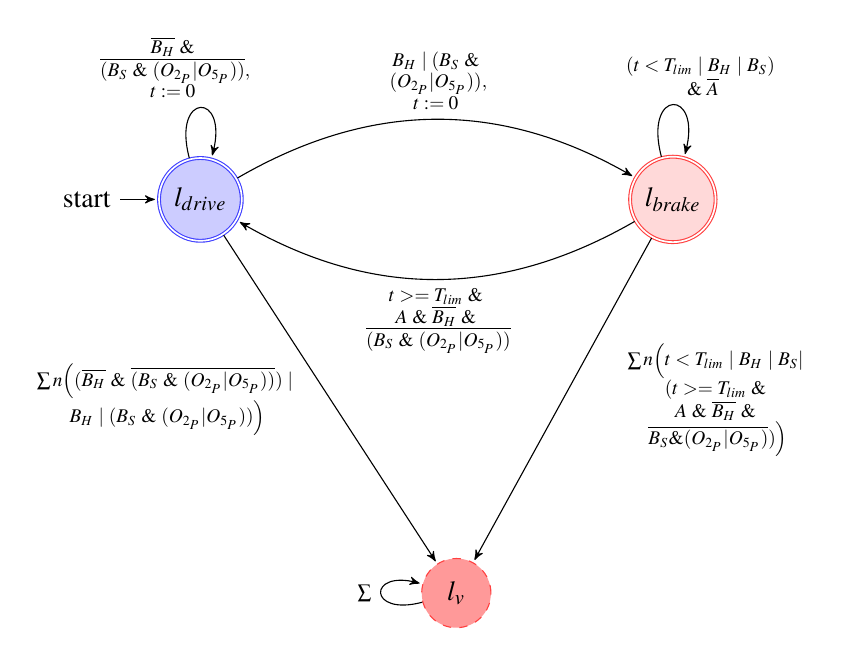
\begin{tikzpicture}[>=stealth',shorten >=1pt,auto,node distance=6 cm, scale = 1, transform shape]

\tikzstyle{accept} = [draw=blue!75,fill=blue!20]
\tikzstyle{violate} = [draw=red!75,fill=red!40, dashed]
\tikzstyle{unstable} = [draw=red!75,fill=red!15]

\node[state, initial, accepting, accept] (A) {$l_{drive}$};
\node[state, accepting, accept, unstable] (B) [right of=A] {$l_{brake}$};
\node[state, violate]         (C) [below of=B, yshift=1cm, xshift=-2.75cm]  {$l_v$};

\path[->] 
		(A) edge [loop above]       node [above, xshift=-1em]  
		{
			\scriptsize$\let\scriptstyle\textstyle\substack{\overline{B_H}~\&\\~ \overline{(B_S~\&~(O_{2_P} | O_{5_P}))}, \\ t := 0}$
		} (A)
		
		(A) edge [bend left]		node [above]  
		{
			\scriptsize$\let\scriptstyle\textstyle\substack{B_H~|~(B_S~\&\\~(O_{2_P} | O_{5_P})), \\ t := 0}$
		} (B)
	
		(A) edge [right]	node [left, xshift=-1em]  
		{
			\scriptsize$\let\scriptstyle\textstyle\substack{\sum\textbackslash \Big((\overline{B_H}~\&~\overline{(B_S~\&~(O_{2_P} | O_{5_P}))})~|\\~B_H~|~(B_S~\&~(O_{2_P} | O_{5_P}))\Big)}$
		} (C)
	
		(B) edge [loop above]		node [above, xshift=1em]  
		{
			\scriptsize$\let\scriptstyle\textstyle\substack{(t < T_{lim}~|~B_H~|~B_S) \\~\&~\overline{A}}$
		} (B)
	
		(B) edge [bend left]				node [below]  
		{
			\scriptsize$\let\scriptstyle\textstyle\substack{t >= T_{lim}~\& \\ A~\&~\overline{B_H}~\&\\~\overline{(B_S~\&~(O_{2_P} | O_{5_P}))}}$
		} (A)
		
		(B) edge [left]			node [right, xshift=2em]  
		{
			\scriptsize$\let\scriptstyle\textstyle\substack{\sum\textbackslash \Big(t < T_{lim}~|~B_H~|~B_S|\\(t >= T_{lim}~\& \\ A~\&~\overline{B_H}~\&\\~\overline{B_S \& (O_{2_P} | O_{5_P})})\Big)}$
		} (C)
	
		(C) edge [loop left]		node [left]  
		{
			\scriptsize$\sum$
		} (C)
		;

\end{tikzpicture}
%\end{filecontents*}
%\begin{filecontents*}{avcarrte.tikz}
%	

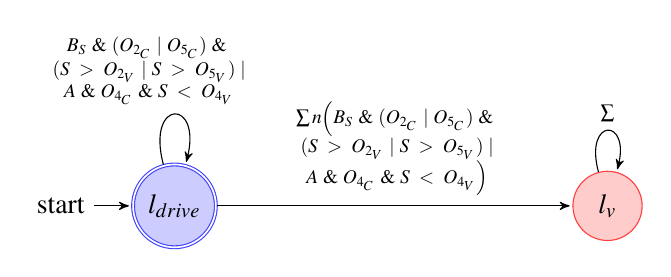
\begin{tikzpicture}[>=stealth',shorten >=1pt,auto,node distance=5.5 cm, scale = 1, transform shape]

\tikzstyle{accept} = [draw=blue!75,fill=blue!20]
\tikzstyle{violate} = [draw=red!75,fill=red!20]

\node[initial,state, accepting, accept] (A) {$l_{drive}$};
\node[state, violate]         (C) [right of=A]  {$l_v$};

\path[->] 
		(A) edge [loop above]       node [above, xshift=-1em]  
		{
			\scriptsize$\let\scriptstyle\textstyle\substack{B_S~\&~(O_{2_C}~|~O_{5_C})~\&\\~(S~>~O_{2_V}~|~S~>~O_{5_V})~|\\~A~\&~O_{4_C}~\&~S~<~O_{4_V}}$
		} (A)
	
		(A) edge [right]	node [above]  
		{
			\scriptsize$\let\scriptstyle\textstyle\substack{\sum\textbackslash \Big(B_S~\&~(O_{2_C}~|~O_{5_C})~\&\\~(S~>~O_{2_V}~|~S~>~O_{5_V})~|\\~A~\&~O_{4_C}~\&~S~<~O_{4_V}\Big)}$
		} (C)
	
		(C) edge [loop above]		node [above]  
		{
			\scriptsize$\sum$
		} (C)
		;

\end{tikzpicture}
%\end{filecontents*}
%\begin{filecontents*}{avdriverte.tikz}
%	

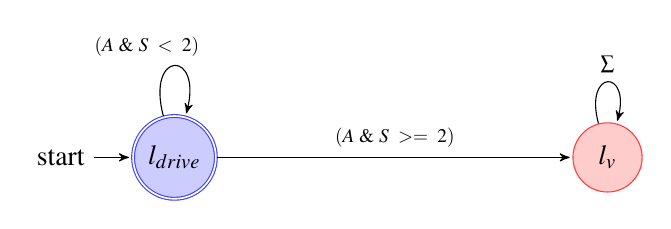
\begin{tikzpicture}[>=stealth',shorten >=1pt,auto,node distance=5.5 cm, scale = 1, transform shape]

\tikzstyle{accept} = [draw=blue!75,fill=blue!20]
\tikzstyle{violate} = [draw=red!75,fill=red!20]

\node[initial,state, accepting, accept] (A) {$l_{drive}$};
\node[state, violate]         (C) [right of=A]  {$l_v$};

\path[->] 
(A) edge [loop above]       node [above, xshift=-1em]  
{
	\scriptsize$\let\scriptstyle\textstyle\substack{(A~\&~S~<~2)}$
} (A)

(A) edge [right]	node [above]  
{
	\scriptsize$\let\scriptstyle\textstyle\substack{(A~\&~S~>=~2)}$
} (C)

(C) edge [loop above]		node [above]  
{
	\scriptsize$\sum$
} (C)
;

\end{tikzpicture}
%\end{filecontents*}
%\begin{filecontents*}{avcnnrte.tikz}
%	

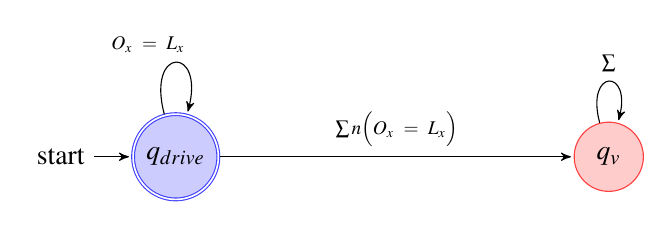
\begin{tikzpicture}[>=stealth',shorten >=1pt,auto,node distance=5.5 cm, scale = 1, transform shape]

\tikzstyle{accept} = [draw=blue!75,fill=blue!20]
\tikzstyle{violate} = [draw=red!75,fill=red!20]

\node[initial,state, accepting, accept] (A) {$q_{drive}$};
\node[state, violate]         (C) [right of=A]  {$q_v$};

\path[->] 
(A) edge [loop above]       node [above, xshift=-1em]  
{
	\scriptsize$\let\scriptstyle\textstyle\substack{O_x~=~L_x}$
} (A)

(A) edge [right]	node [above]  
{
	\scriptsize$\let\scriptstyle\textstyle\substack{\sum\textbackslash \Big(O_x~=~L_x\Big)}$
} (C)

(C) edge [loop above]		node [above]  
{
	\scriptsize$\sum$
} (C)
;

\end{tikzpicture}
%\end{filecontents*}

\begin{filecontents*}{avgraph.tikz}
	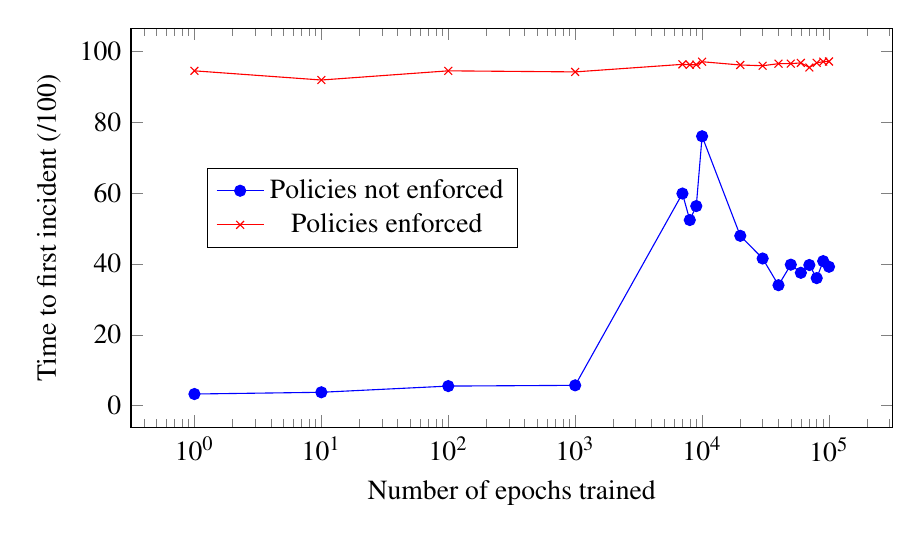
\begin{tikzpicture}
\begin{semilogxaxis}[
xlabel={Number of epochs trained},
ylabel={Time to first incident (/100)},
x=0.7cm,
y=0.45mm, 
legend style={at={(0.1,0.55)},anchor=west}]

\addplot[color=blue,mark=*] coordinates {
	(0, 3.24)
	(1, 3.29)
	(10, 3.78)
	(100, 5.53)
	(1000, 5.74)
	(7000, 59.87)
	(8000, 52.39)
	(9000, 56.33)
	(10000, 76.03)
	(20000, 47.94)
	(30000, 41.54)
	(40000, 34)
	(50000, 39.8)
	(60000, 37.5)
	(70000, 39.7)
	(80000, 36)
	(90000, 40.8)
	(100000, 39.2)
};

\addplot[color=red,mark=x] coordinates {
	(0, 93.2)
	(1, 94.5)
	(10, 91.91)
	(100, 94.5)
	(1000, 94.2)
	(7000, 96.33)
	(8000, 96.21)
	(9000, 96.24)
	(10000, 97.07)
	(20000, 96.15)
	(30000, 95.94)
	(40000, 96.52)
	(50000, 96.53)
	(60000, 96.74)
	(70000, 95.44)
	(80000, 96.75)
	(90000, 97.09)
	(100000, 97.14)
};

\legend{Policies not enforced, Policies enforced}
\end{semilogxaxis}%
\end{tikzpicture}%
\end{filecontents*}
\begin{filecontents*}{avpedrte.tikz}


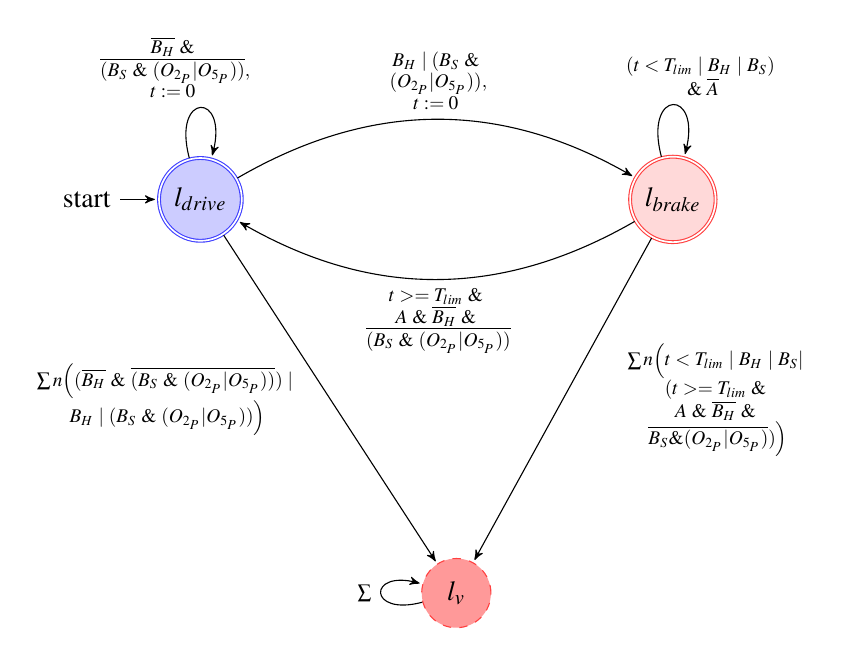
\begin{tikzpicture}[>=stealth',shorten >=1pt,auto,node distance=6 cm, scale = 1, transform shape]

\tikzstyle{accept} = [draw=blue!75,fill=blue!20]
\tikzstyle{violate} = [draw=red!75,fill=red!40, dashed]
\tikzstyle{unstable} = [draw=red!75,fill=red!15]

\node[state, initial, accepting, accept] (A) {$l_{drive}$};
\node[state, accepting, accept, unstable] (B) [right of=A] {$l_{brake}$};
\node[state, violate]         (C) [below of=B, yshift=1cm, xshift=-2.75cm]  {$l_v$};

\path[->] 
		(A) edge [loop above]       node [above, xshift=-1em]  
		{
			\scriptsize$\let\scriptstyle\textstyle\substack{\overline{B_H}~\&\\~ \overline{(B_S~\&~(O_{2_P} | O_{5_P}))}, \\ t := 0}$
		} (A)
		
		(A) edge [bend left]		node [above]  
		{
			\scriptsize$\let\scriptstyle\textstyle\substack{B_H~|~(B_S~\&\\~(O_{2_P} | O_{5_P})), \\ t := 0}$
		} (B)
	
		(A) edge [right]	node [left, xshift=-1em]  
		{
			\scriptsize$\let\scriptstyle\textstyle\substack{\sum\textbackslash \Big((\overline{B_H}~\&~\overline{(B_S~\&~(O_{2_P} | O_{5_P}))})~|\\~B_H~|~(B_S~\&~(O_{2_P} | O_{5_P}))\Big)}$
		} (C)
	
		(B) edge [loop above]		node [above, xshift=1em]  
		{
			\scriptsize$\let\scriptstyle\textstyle\substack{(t < T_{lim}~|~B_H~|~B_S) \\~\&~\overline{A}}$
		} (B)
	
		(B) edge [bend left]				node [below]  
		{
			\scriptsize$\let\scriptstyle\textstyle\substack{t >= T_{lim}~\& \\ A~\&~\overline{B_H}~\&\\~\overline{(B_S~\&~(O_{2_P} | O_{5_P}))}}$
		} (A)
		
		(B) edge [left]			node [right, xshift=2em]  
		{
			\scriptsize$\let\scriptstyle\textstyle\substack{\sum\textbackslash \Big(t < T_{lim}~|~B_H~|~B_S|\\(t >= T_{lim}~\& \\ A~\&~\overline{B_H}~\&\\~\overline{B_S \& (O_{2_P} | O_{5_P})})\Big)}$
		} (C)
	
		(C) edge [loop left]		node [left]  
		{
			\scriptsize$\sum$
		} (C)
		;

\end{tikzpicture}
\end{filecontents*}
\begin{filecontents*}{avcarrte.tikz}


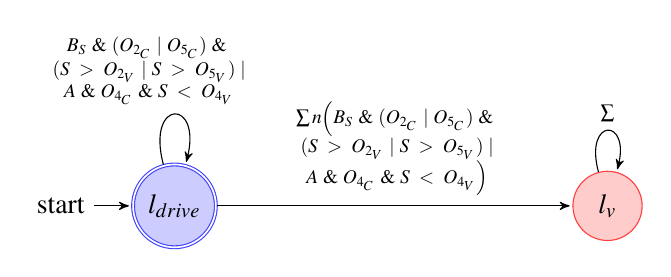
\begin{tikzpicture}[>=stealth',shorten >=1pt,auto,node distance=5.5 cm, scale = 1, transform shape]

\tikzstyle{accept} = [draw=blue!75,fill=blue!20]
\tikzstyle{violate} = [draw=red!75,fill=red!20]

\node[initial,state, accepting, accept] (A) {$l_{drive}$};
\node[state, violate]         (C) [right of=A]  {$l_v$};

\path[->] 
		(A) edge [loop above]       node [above, xshift=-1em]  
		{
			\scriptsize$\let\scriptstyle\textstyle\substack{B_S~\&~(O_{2_C}~|~O_{5_C})~\&\\~(S~>~O_{2_V}~|~S~>~O_{5_V})~|\\~A~\&~O_{4_C}~\&~S~<~O_{4_V}}$
		} (A)
	
		(A) edge [right]	node [above]  
		{
			\scriptsize$\let\scriptstyle\textstyle\substack{\sum\textbackslash \Big(B_S~\&~(O_{2_C}~|~O_{5_C})~\&\\~(S~>~O_{2_V}~|~S~>~O_{5_V})~|\\~A~\&~O_{4_C}~\&~S~<~O_{4_V}\Big)}$
		} (C)
	
		(C) edge [loop above]		node [above]  
		{
			\scriptsize$\sum$
		} (C)
		;

\end{tikzpicture}
\end{filecontents*}
\begin{filecontents*}{avdriverte.tikz}


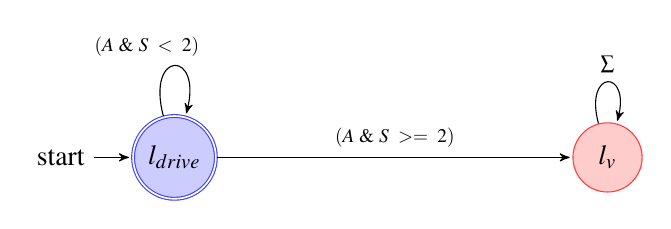
\begin{tikzpicture}[>=stealth',shorten >=1pt,auto,node distance=5.5 cm, scale = 1, transform shape]

\tikzstyle{accept} = [draw=blue!75,fill=blue!20]
\tikzstyle{violate} = [draw=red!75,fill=red!20]

\node[initial,state, accepting, accept] (A) {$l_{drive}$};
\node[state, violate]         (C) [right of=A]  {$l_v$};

\path[->] 
(A) edge [loop above]       node [above, xshift=-1em]  
{
	\scriptsize$\let\scriptstyle\textstyle\substack{(A~\&~S~<~2)}$
} (A)

(A) edge [right]	node [above]  
{
	\scriptsize$\let\scriptstyle\textstyle\substack{(A~\&~S~>=~2)}$
} (C)

(C) edge [loop above]		node [above]  
{
	\scriptsize$\sum$
} (C)
;

\end{tikzpicture}
\end{filecontents*}
\begin{filecontents*}{avcnnrte.tikz}


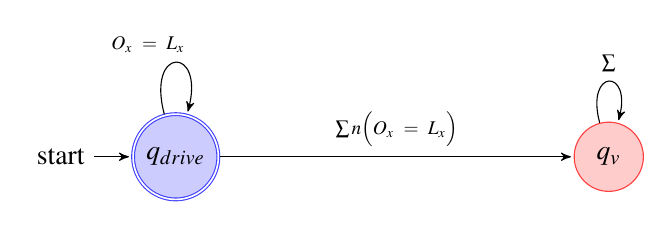
\begin{tikzpicture}[>=stealth',shorten >=1pt,auto,node distance=5.5 cm, scale = 1, transform shape]

\tikzstyle{accept} = [draw=blue!75,fill=blue!20]
\tikzstyle{violate} = [draw=red!75,fill=red!20]

\node[initial,state, accepting, accept] (A) {$q_{drive}$};
\node[state, violate]         (C) [right of=A]  {$q_v$};

\path[->] 
(A) edge [loop above]       node [above, xshift=-1em]  
{
	\scriptsize$\let\scriptstyle\textstyle\substack{O_x~=~L_x}$
} (A)

(A) edge [right]	node [above]  
{
	\scriptsize$\let\scriptstyle\textstyle\substack{\sum\textbackslash \Big(O_x~=~L_x\Big)}$
} (C)

(C) edge [loop above]		node [above]  
{
	\scriptsize$\sum$
} (C)
;

\end{tikzpicture}
\end{filecontents*}

\begin{filecontents*}{avgraph.tikz}
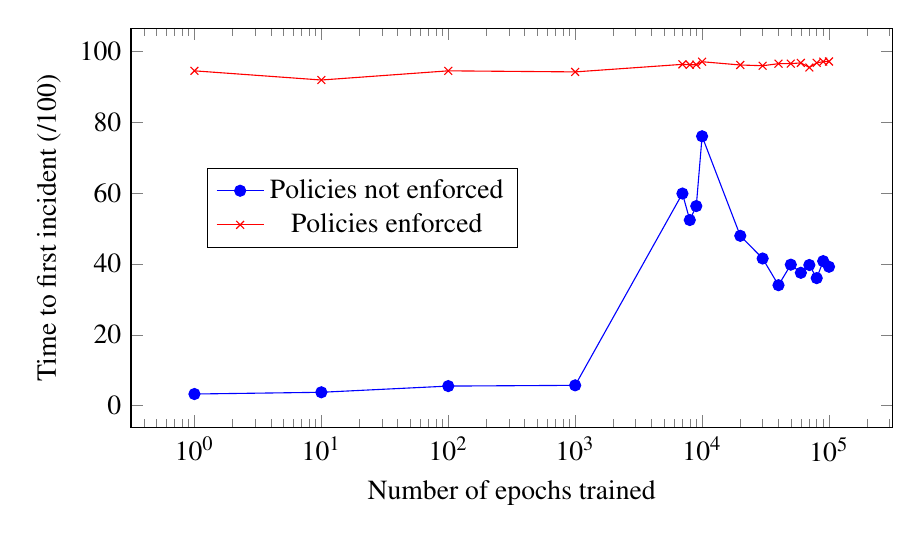
\begin{tikzpicture}
\begin{semilogxaxis}[
xlabel={Number of epochs trained},
ylabel={Time to first incident (/100)},
x=0.7cm,
y=0.45mm, 
legend style={at={(0.1,0.55)},anchor=west}]

\addplot[color=blue,mark=*] coordinates {
	(0, 3.24)
	(1, 3.29)
	(10, 3.78)
	(100, 5.53)
	(1000, 5.74)
	(7000, 59.87)
	(8000, 52.39)
	(9000, 56.33)
	(10000, 76.03)
	(20000, 47.94)
	(30000, 41.54)
	(40000, 34)
	(50000, 39.8)
	(60000, 37.5)
	(70000, 39.7)
	(80000, 36)
	(90000, 40.8)
	(100000, 39.2)
};

\addplot[color=red,mark=x] coordinates {
	(0, 93.2)
	(1, 94.5)
	(10, 91.91)
	(100, 94.5)
	(1000, 94.2)
	(7000, 96.33)
	(8000, 96.21)
	(9000, 96.24)
	(10000, 97.07)
	(20000, 96.15)
	(30000, 95.94)
	(40000, 96.52)
	(50000, 96.53)
	(60000, 96.74)
	(70000, 95.44)
	(80000, 96.75)
	(90000, 97.09)
	(100000, 97.14)
};

\legend{Policies not enforced, Policies enforced}
\end{semilogxaxis}%
\end{tikzpicture}%
\end{filecontents*}

\begin{document}

\title{Synchronous Neural Networks for Cyber-Physical Systems}
\author{Keyan Themba Monadjem}
\department{Electrical \& Computer Engineering}
\submitdate{February 2019}
\supervisor[Dr. Partha S. Roop]{}

%create the title page
\maketitle

%%%%%%%%%%%%% First section %%%%%%%%%%%%%%%
\frontmatter
\bookmark[page=3]{Abstract}
\begin{abstract}
Cyber-physical systems (CPS), such as autonomous vehicles or smart power grids, use interactive machine learning modules for decision making. Current design approaches use multiple machine learning modules, often using Artificial Neural Networks (ANNs), to achieve the desired functionality. Current approaches to verification and validation of these ANNs are generally either very difficult, time consuming and/or not fully reliable. A key feature missing is related to the use of ANNs in real-time systems, which demand the capability of worst-case analysis. 
In this thesis we introduce Synchronous Neural Networks (SNNs) as a new approach to the safe use of ANNs in CPS. SNNs provide synchronous semantics to ANNs. This enables real-time operation and facilitates static timing analysis of individual ANNs. We define these SNNs the Esterel synchronous language. We then use a time predictable platform called T-CREST, which facilitates static timing analysis.

We propose Meta Neural Networks (MNNs) as a framework for the systematic composition of SNNs. This enables compositional system design using multiple SNNs and other synchronous functional components, while maintaining the synchronous semantics of the system. Synchronous MNNs allow for the creation of causal, deterministic, predictable controllers for CPS. 

Misclassification is a major issue with input perturbation in ANNs. We combine MNNs with Run-time Enforcers (RE), which enforce a set of desired policies by transforming inputs and outputs suitably. The proposed solution is able to effectively deal with many misclassifications.
Finally, we propose a tool that extends the ANN-library Keras to give it a MNN description capability. We then automatically generate synchronous C code, which is shown to perform even better than our earlier MNN implementation using Esterel. 

We have developed several CPS examples that range from an energy storage system for charging electric vehicles, to a traffic sign detection system for autonomous vehicles. These results show that the implemented MNNs can meet real-time, safety critical deadlines. Composing MNNs of multiple SNNs and RE provide an increase in the safety of autonomous vehicles, where the MNNs not only increase classification accuracy of the environment, but also detect misclassifications and allow the system to respond safely to these misclassifications. 
\end{abstract}


\renewcommand{\abstractname}{Acknowledgements}

\bookmark[page=5]{Acknowledgements}
\begin{abstract}
	Firstly, I would like to express my very great appreciation to my supervisor, Partha S. Roop. 
	He expended a lot of time and a lot of effort to get me to the point where I am now, and I am exceedingly grateful for that.
	He guided me through the tenure of my thesis, showing me what needed to be done, but not doing it for me.
	I learned many new and interesting concepts and technologies while working with him and was able to produce a great thesis with original work.
	
	Second is Hammond Pearce. 
	I am very thankful for the help from Mr. Hammond Pearce, PhD student at the University of Auckland.
	He took the role as a secondary supervisor to me, even with his own work as a PhD student.
	He helped me many a time when I was stuck, had a question or needed a push in the right direction.
	
	Next is the EECE group from the University of Auckland. 
	Many thanks to Matthew Kuo, Nathan Allen and Jin Ro.
	All three gentlemen helped me numerous times during my time as a ME student.
	
	A thanks to Yash Raje, who was a great lab partner and someone I spent a lot of time working with.
	
	Without Marc Katzef, University of Canterbury, I would not have been able to use the extremely well made MNN2C tool.
	He did a really great job creating it in his time spent at the University of Auckland, and I would like to thank him for his fantastic work.
	
	Finally, I wish to thank my family; my mom, my dad, my stepmom, my aunt, my brothers, and last, but not least, a friend of many years. 
	They all supported me throughout this degree and gave me the love and encouragement I needed.
	
\end{abstract}

%create table of contents
\bookmark[page=7]{Contents} % Sets a PDF bookmark for the contents page
\tableofcontents

\bookmark[page=11]{List of Figures}
\listoffigures

\bookmark[page=15]{List of Tables}
\listoftables

%\cleardoublepage
%\phantomsection
%\addcontentsline{toc}{chapter}{List of Abbreviations}
%\input{abbreviations}

%%%%%%%%%%%% Body of the Thesis %%%%%%%%%%%
\mainmatter

\acrodef{WCRT}{Worst Case Reaction Time}
\acrodef{WCET}{Worst Case Execution Time}
\acrodef{SOT}{Start Of Tick}
\acrodef{EOT}{End Of Tick}
\acrodef{CPS}{Cyber-Physical System}
\acrodef{AI}{Artificial Intelligence}

\acrodef{ESS}{Energy Storage System}
\acrodef{SoC}{State of Charge}
\acrodef{MBD}{Model-Based Design}
\acrodef{FPGA}{Field-Programmable Gate Array}

\acrodef{CFG}{Control Flow Graph}
\acrodef{TCFG}{Timed Control Flow Graph}
\acrodef{TCCFG}{Timed Concurrent Control Flow Graph}
\acrodef{TCA}{Tick Cost Automata}

\acrodef{SMT}{Satisfiability Modulo Theories}

\acrodef{NN}{Neural Network}
\acrodef{DNN}{Deep Neural Network}
\acrodef{SNN}{Synchronous Neural Network}
\acrodef{CNN}{Convolutional Neural Network}
\acrodef{SANN}{Synchronous Artificial Neural Network}
\acrodef{SNN}{Synchronous Neural Network}
\acrodef{SSNN}{Safe Synchronous Neural Network}
\acrodef{ANN}{Artificial Neural Network}
\acrodef{RNN}{Recurrent Neural Network}
\acrodef{MLP}{Multi-layer Perceptron}
\acrodef{MNN}{Meta Neural Network}
\acrodef{MNN2C}{Meta Neural Network to C}

\acrodef{AV}{Autonomous Vehicle}
\acrodef{LiDAR}{Light Detection and Ranging}

\acrodef{VOC}{Visual Object Classes}
\acrodef{GTSRB}{German Traffic Sign Recognition Benchmark}

\acrodef{VDTA}{Valued Discrete Timed Automata}
\acrodef{DTA}{Discrete Timed Automata}
\acrodef{RE}{Runtime Enforcement}
\acrodef{RA}{Runtime Assurance}
\acrodef{RV}{Runtime Verification}

\chapter{Introduction}

\section{\acf{CPS}}
\acf{CPS} refer to a network of distributed controllers that manage the physical processes of the system~\cite{cps-design}~\cite{alur2015principles}. 
\ac{CPS} encompass a wide variety of disciplines, from mechatronics to civil infrastructure (Figure~\ref{fig:cps}).
\ac{CPS} operate in the physical world, where environments can be unpredictable and uncontrolled.
This introduces safety concerns for the \ac{CPS}; the hardware must be predictable and reliable, and the software must be predictable and reliable.
This thesis focuses on the software requirements for \ac{CPS}.

\begin{figure}[h]
	\centering
	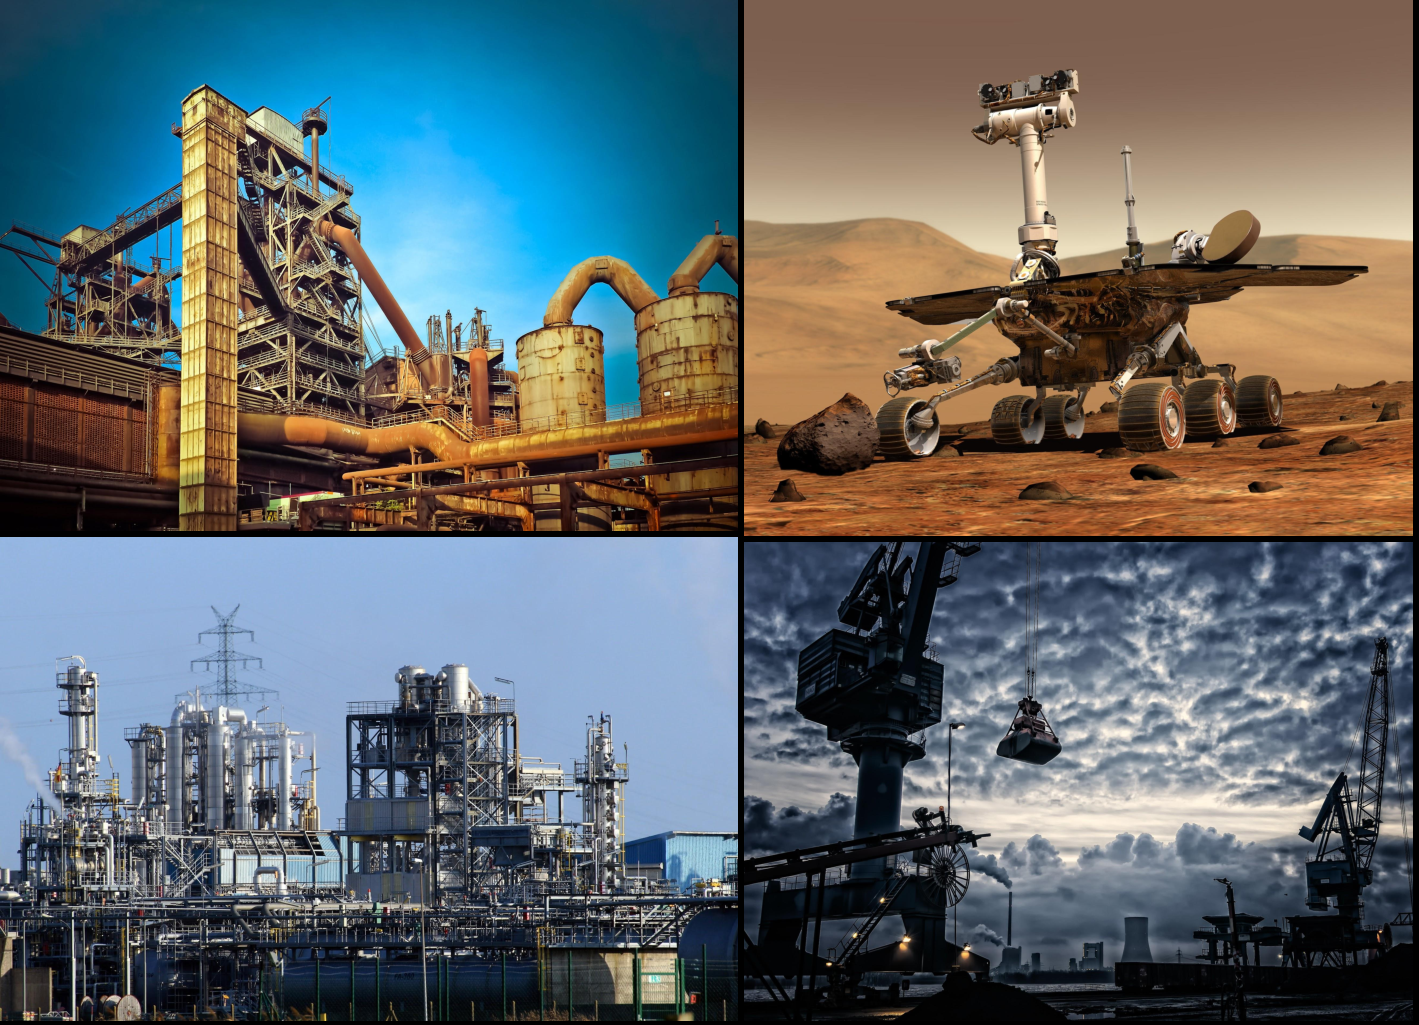
\includegraphics[width=\textwidth]{Content/fig/1234.pdf}
	\caption{Examples of \ac{CPS}~\cite{industry-pic}~\cite{crane-pic}~\cite{rover-pic}~\cite{factory-pic}, from left to right, top to bottom: A) factories, B) robotics, C) power and electricity, and D) construction \label{fig:cps}}
\end{figure}

\ac{CPS} applications encompass real-time systems, where the systems need to satisfy a set of timing and functional requirements to ensure correct operation. 
Here, a missed deadline may result in catastrophic consequences, making these \ac{CPS} highly \textit{safety-critical}. 
These have strict timing and functionality requirements --- any errors in control can result in physical damage, injuries, and/or fatalities~\cite{ANNDevModel1999}. 


\section{\acf{AI} and \acf{ML}}
\acf{ML} is a field of data science where \acfp{AI} are taught to learn large and/or complex data relationships~\cite{ai}.
\ac{AI} come in many shapes and forms, from decision trees to \acfp{ANN}~\cite{ai-types}.
\ac{AI} were invented to fill a gap that humans cannot, where they can store a huge number of data relationships and learn new relationships where a person would struggle.
\ac{AI} are used all over industry, from industrial systems, to cybernetics and robotics (such as Figure~\ref{fig:ai-girl}).

\begin{figure}[h]
	\centering
	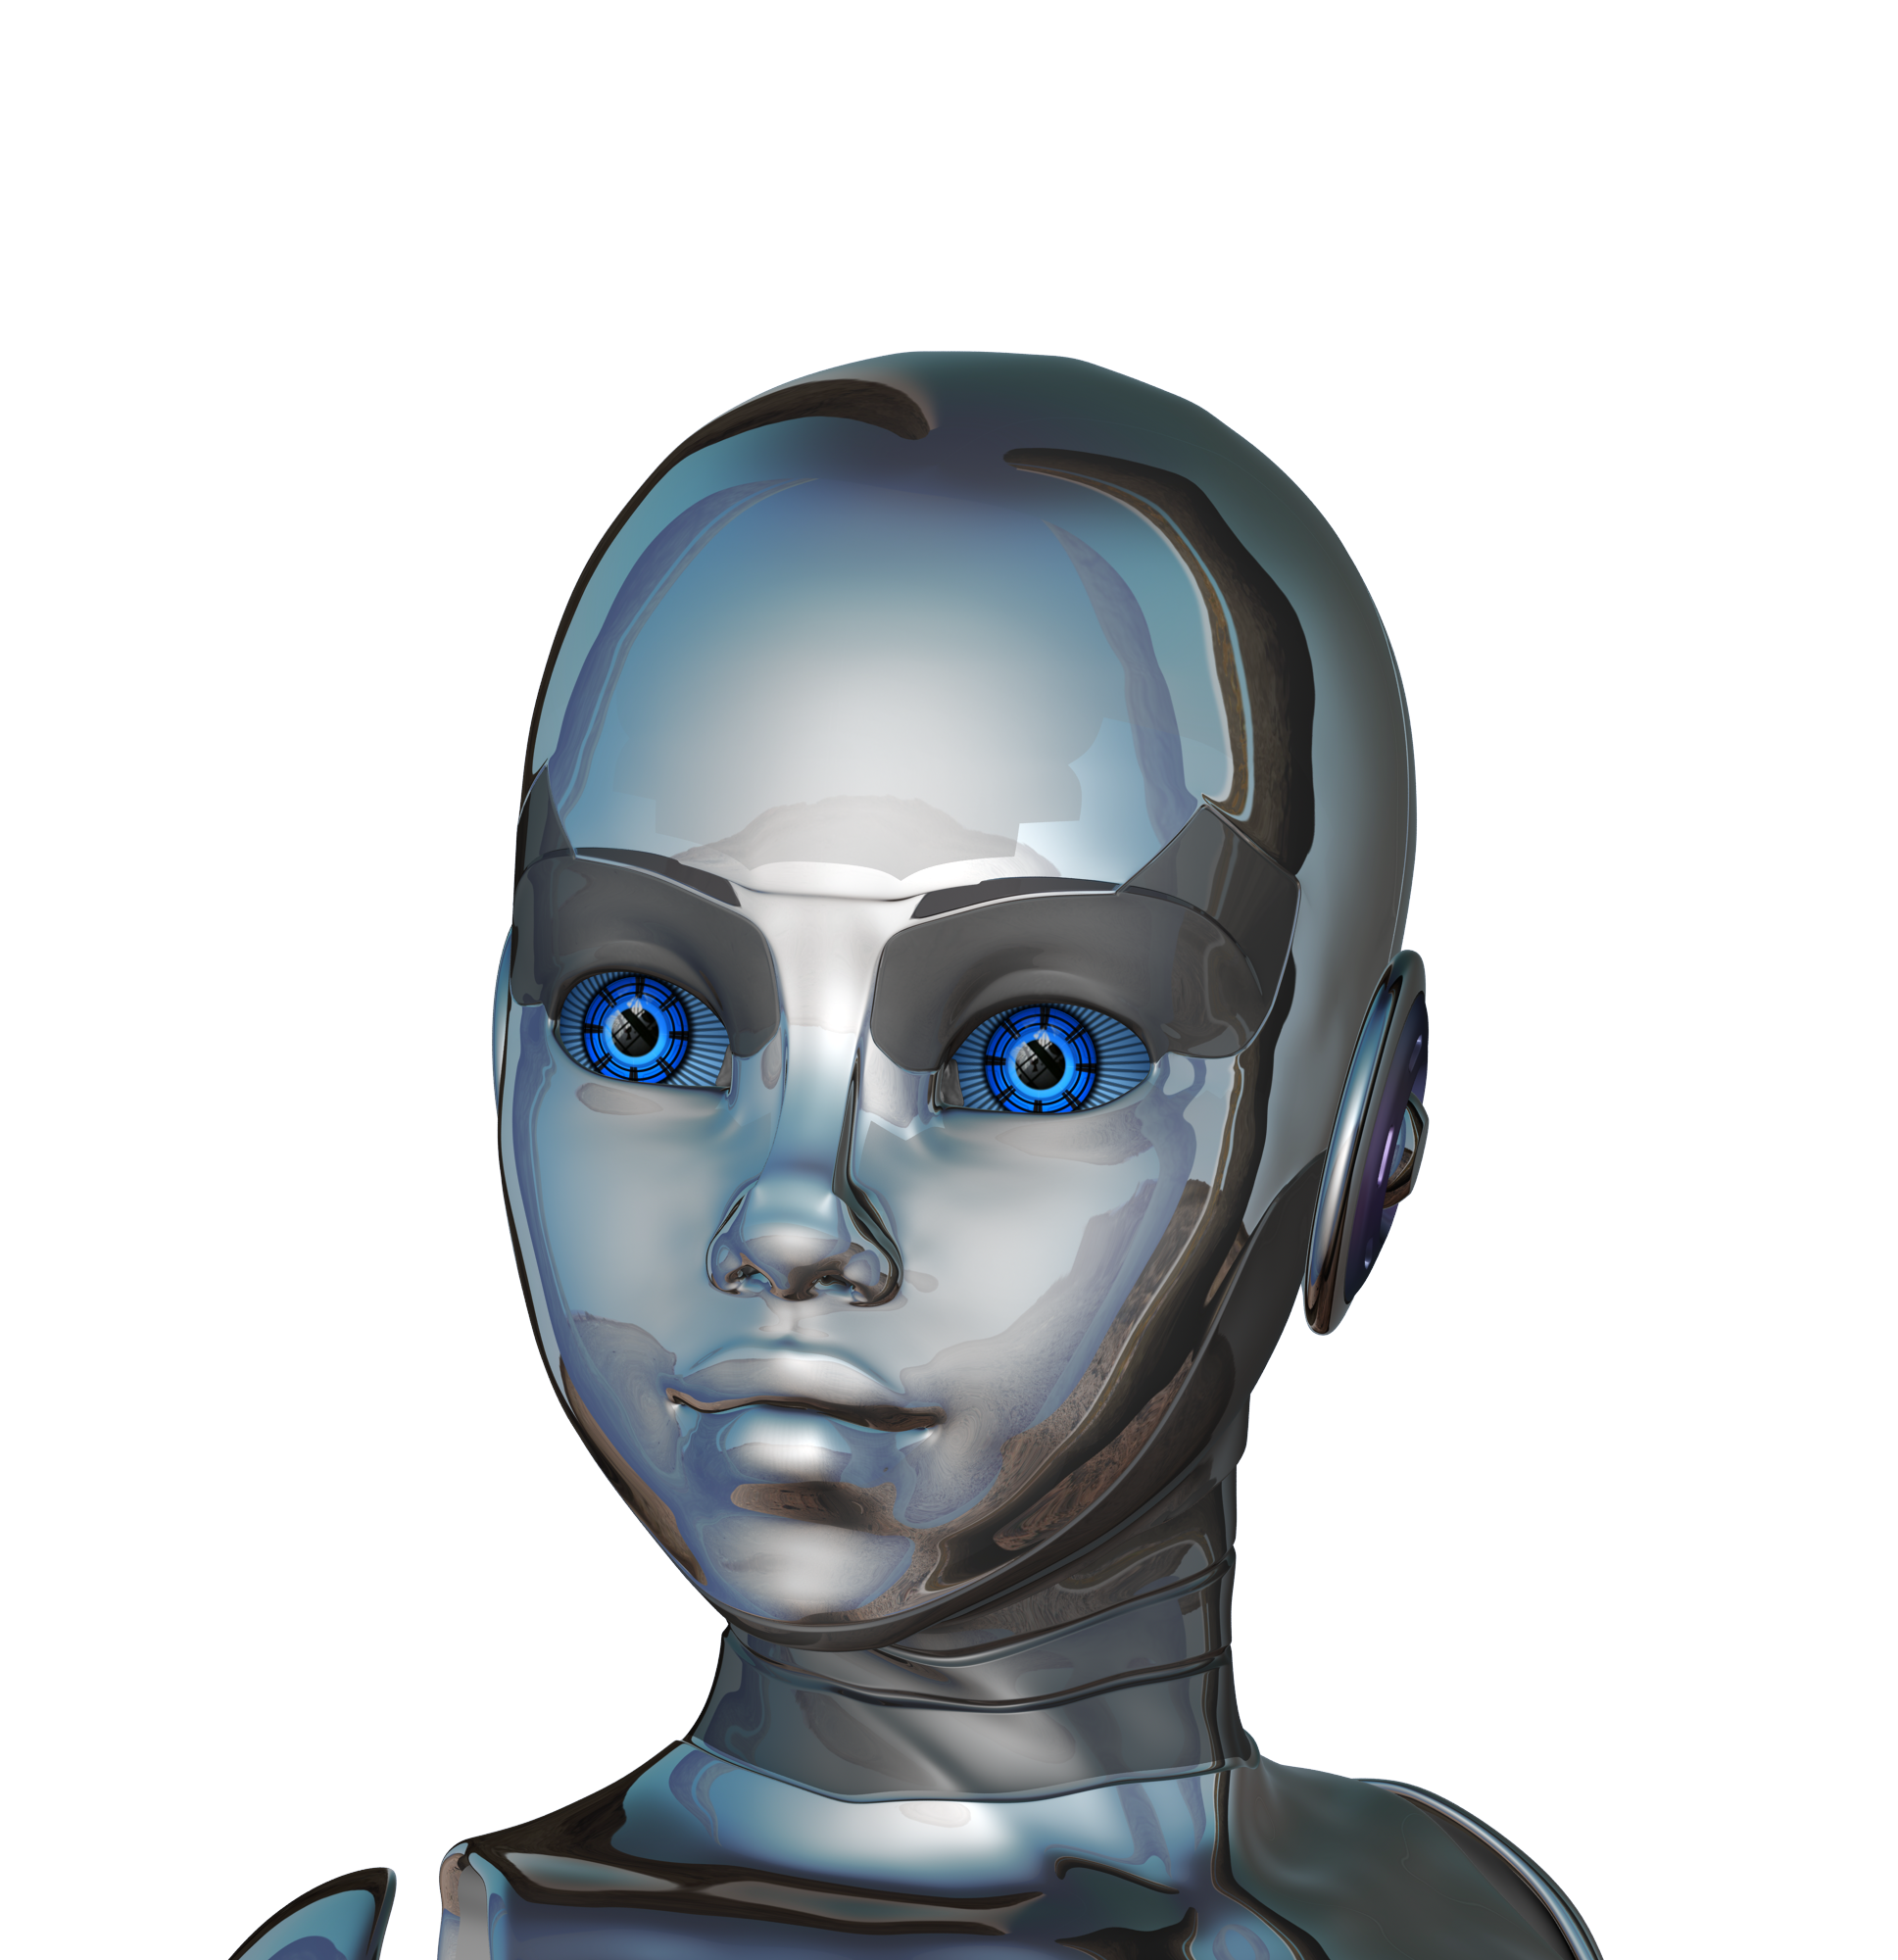
\includegraphics[width=0.4\textwidth]{Content/fig/ai-girl.png}
	\caption{\acp{AI} are frequently used as the controllers of robots~\cite{robotgirl-pic} \label{fig:ai-girl}}
\end{figure}

\ac{AI} are increasingly used in \ac{CPS}, where safety is critical.
However, the mathematical nature of \ac{AI} is non-linear, leaving many \ac{AI} difficult to verify and validate.
Additionally, as \ac{AI} adapt to learn larger data sets and more complex relationships, the size and complexity of the \acp{AI} increase.
Some of these \acp{AI} are easier to verify and validate than others~\cite{aiverify} however, as they grow in size, these techniques take more time and other resources to implement.
In \ac{CPS}, it is essential for all components to be verified and validated, and thus the issue with \ac{AI} in \ac{CPS} is made clear: conventional techniques cannot be used to verify \acp{AI} for \ac{CPS}.

\subsection{\acfp{ANN}}
\acp{ANN} are a type of \ac{AI} designed to model the functionality of the human brain~\cite{kohonen1988introduction}.
The resulting \acp{ANN} are generally large and complex.
They are composed of layers interconnected artificial neurons, each neuron passing numerical messages along to the next, and can be represented mathematically by a complex, non-linear equation.
They are able to store large and complex data relationships~\cite{ANNSafety2007}, like their biological counterpart, and this is where they are most useful.
However, the result is that \acp{ANN} are extremely difficult to verify or validate~\cite{menzies2005verification}.

\acp{ANN} are often used in big data and Internet of Things (IoT), but also show up in \ac{CPS} such as \acfp{AV}.
Their use in \ac{CPS} is highly contended, as \acp{ANN} are not 100\% reliable and accidents happen~\cite{coldewey_2018}.
Thus, it is of utmost importance that any \ac{ANN} used in any \ac{CPS} is verified to be safe for that system in all possible environments.
Without that guarantee of safety the use of \ac{AI} in such systems is risky and an endangerment to any person involved with the system and its environment~\cite{ANNSafety2018}.
There exists a large body of research dealing with the safety of \acp{ANN}, but there are plenty of opportunities for research towards safe \acp{ANN}.

\section{Contribution}
This thesis provides novel techniques to the verification and validation of \acfp{ANN} in \acf{CPS}.
There is a large body of work regarding the safety of \acp{ANN}, ranging across a whole variety of applications and approaches.
However, no work has been done regarding the synchronous implementation of \acp{ANN} and the verification available to synchronous \acp{ANN}, which we term \acfp{SNN}.  
This thesis addresses the issue of safe \acp{ANN} using synchronous semantics~\cite{berry1991}.

In this thesis, a new \ac{ANN} library was created to demonstrate the benefits of synchronous \acp{ANN}.
In the benchmarks using deep \acp{ANN}, an existing library called Darknet~\cite{darknet13} was used to implement the deep \acp{ANN}.
However, a tool chain was created to replace Darknet that compiles Keras~\cite{chollet2015keras} trained \acp{ANN} to the created \ac{ANN} library.

The major contributions of this thesis are as follows:
\begin{itemize}
	\item A time predictable approach to \acp{ANN} is developed using the synchronous language Esterel~\cite{berry2000foundations}. These predictable \acp{ANN} are termed \acfp{SNN} and are defined using formal methods. Using T-CREST's Patmos processor architecture~\cite{patmos:ppes2011}, timing analysis of these \acp{SNN} is possible. These \acp{SNN} provide a safe approach to implementing \acp{ANN} in \ac{CPS}. The results of the \acp{SNN} are presented using a set of benchmarks. 
	\item \acfp{MNN} are proposed as a framework for the composition of multiple \acp{SNN}. The thesis provides formal definitions for the \acp{MNN} and benchmarks are presented that show their efficacy. 
	\item The combination of \acf{RE} and \acp{SNN} is investigated, with the intent to modify unsafe events. This provides functional safety for \acp{SNN}, something not covered in previous chapters. An \acf{AV} case study is introduced for the purposes of this work and a simulation is created to demonstrate its efficacy.
	\item \acf{RV} of \acp{MNN} is proposed as an approach to dealing with input perturbation. This demonstrates a functional verification method for \acp{ANN} that have complex inputs, such as image classification \acfp{CNN}, where \ac{RE} is not an option. An \ac{AV} case study is also created for this work, with an \ac{AV} object detection simulation created to demonstrate the benefits of this proposition. 
\end{itemize}

\section{Thesis Structure}
This chapter, Chapter 1, introduces the problem statement, provides some background to the problem and then introduces the approach this work takes to address the problem.

Chapter 2 gives a basic understanding of the concepts required to understand this research towards safe \acp{ANN} for \ac{CPS}.

Chapter 3 introduces the concept of \acfp{SNN} and their timing properties.
Formal definitions of \acp{SNN} and their related components are provided in Chapter 3.
Furthermore, the meta combinations of these \acp{SNN}, termed \acp{MNN}, and the usefulness of such \acp{MNN} in \ac{CPS} is discussed.
Lastly, a new Python tool chain that creates these \acp{SNN} from Keras is also introduced.

Chapter 4 introduces the concept of \acf{RE} in combination with \acp{SNN}. 
This chapter provides formal definitions for the enforcers and the safety policies that are enforced.
An \acf{AV} case study is made for this chapter to show the efficacy of the \ac{RE} of \acp{SNN}.

Chapter 5 proposes two different methods, used in tandem, to increase the safety of systems with complex inputs, such as object detection for \acp{AV}.
The first method is the use of \acp{MNN} to increase the classification accuracy of \acp{SNN}.
The second expands on Chapter 4, and introduces the use of \ac{RV} to increase the safety of \ac{CPS} where \ac{RE} cannot do so.
An \ac{AV} object detection simulation is created as a complex \ac{MNN} and input perturbation is introduced to the system.
The previous approach to \ac{RE} cannot be used, and as such, \ac{RV} is used to functionally verify this system.

Finally, conclusions are drawn on the synchronous approach proposed in this thesis to creating safe \acp{ANN}.



\chapter{Background and Related Work}

\section{Artificial Neural Networks}
\subsection{Machine Learning}
\acp{ANN} were originally proposed to mimic the functioning of  biological neural networks~\cite{kohonen1988introduction}, which produce recurrent spatio temporal patterns~\cite{rolston2007precisely}. 
Similar timed activity of neurons in the cerebellum has been reported in~\cite{bullock1994neural, moore1989adaptively}. 
A number of types of \ac{NN} which mimic their biological counterparts exist, varying in complexity and accuracy, including the \ac{SNN}~\cite{izhikevich2003spiking,maass1997spiking}, which was designed to model the brain and has been demonstrated to be periodic and run with discrete time intervals when implemented in software. 

\subsection{Structure of an Artificial Neural Network}
Most \acp{ANN} do not feature such complex models like those of spiking neural networks, as they are more difficult to use, implement, and train. 
Instead, they rely on simpler networks, which can be considered as \emph{un-timed non-linear} functions, where the outputs change relative to the inputs, but the timing of the change is not precisely defined. 
An example of such a network is provided in Figure~\ref{fig:mlp-ann}, which is using neurons defined in Figure~\ref{fig:artificial-neuron}. 
This is a type of \ac{NN} known as an \acf{MLP}~\cite{yegnanarayana1994artificial}.

Specialised neural networks, called \acfp{RNN}~\cite{medsker2001recurrent}, were introduced to classify temporal sequences. 
These operate in a step by step manner, where the operation in the current time step relies on the context from some previous step. Thus, \acp{RNN} may be viewed as a periodic networks, whosemperiod is one. 
However, the use of such networks in \ac{CPS} is yet to be thoroughly investigated. 
Moreover, \acp{RNN} and their compositions are not formalised especially from the point of view of designing timed AI systems used in \ac{CPS}.  

\begin{figure}
	\centering
	\scalebox{0.8}{\def\layersep{2.25cm}
\def\numInp{4}
\def\numHid{5}
\def\numOut{3}
\begin{tikzpicture}[shorten >=1pt,->,draw=black!100, node distance=\layersep]
	\tikzstyle{every pin edge}=[<-,shorten <=1pt]
	\tikzstyle{neuron}=[circle,fill=black!25,minimum size=20pt,inner sep=0pt]
	\tikzstyle{input neuron}=[neuron, fill=white!100,draw=black];
	\tikzstyle{output neuron}=[neuron, fill=white!100,draw=black];
	\tikzstyle{hidden neuron}=[neuron, fill=white!100,draw=black];
	\tikzstyle{annot} = [text width=4em, text centered]
	
	% Draw the input layer nodes
	\foreach \name / \y in {1,...,\numInp}
	% This is the same as writing \foreach \name / \y in {1/1,2/2,3/3,4/4}
	\node[input neuron, pin=left:Input \y] (I-\name) at (0,-\y) {$i_\y$};
	
	% Draw the hidden layer nodes
	\foreach \name / \y in {1,...,\numHid}
	\path[yshift=0.5cm]
	node[hidden neuron] (H-\name) at (\layersep,-\y cm) {$h_\y$};
	
	% Draw the output layer nodes
	\foreach \name / \y in {1,...,\numOut}
	\node[output neuron, pin={[pin edge={->}]right:Output \y}] (O-\name) at (4.5,-0.25-\y) {$o_\y$};
		
	% Connect every node in the input layer with every node in the
	% hidden layer.
	\foreach \source in {1,...,\numInp}
	\foreach \dest in {1,...,\numHid}
	\path (I-\source) edge (H-\dest);
	
	% Connect every node in the hidden layer with the output layer
	\foreach \source in {1,...,\numHid}
	\foreach \dest in {1,...,\numOut}
	\path (H-\source) edge (O-\dest);
	
	% Annotate the layers
	\node[annot,above of=H-1, node distance=1cm] (hl) {\textit{Hidden Layer}};
	\node[annot,left of=hl] {\textit{Input Layer}};
	\node[annot,right of=hl] {\textit{Output Layer}};
\end{tikzpicture}}
	\caption{Example \ac{MLP} \ac{ANN}.	\label{fig:mlp-ann}}
\end{figure}
\begin{figure}
	\centering
	\scalebox{0.8}{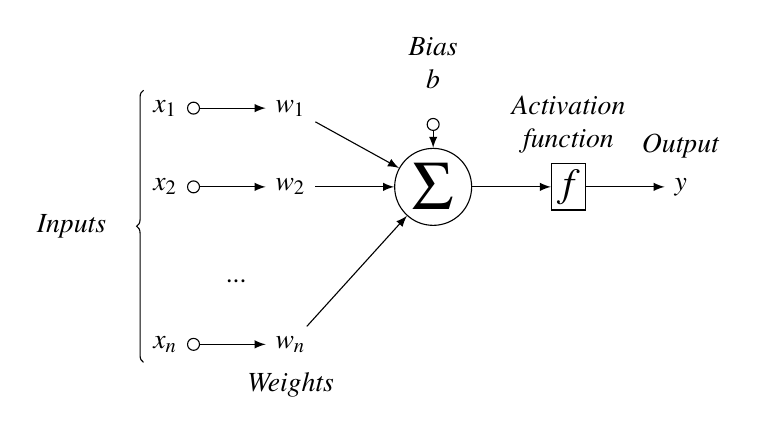
\begin{tikzpicture}[
init/.style={
  draw,
  circle,
  inner sep=2pt,
  font=\Huge\itshape,
  join = by -latex
},
squa/.style={
  draw,
  inner sep=2pt,
  font=\Large,
  join = by -latex
},
start chain=2,node distance=10mm
]
\node[on chain=2] 
  (x2) {$x_2$};
\node[on chain=2,join=by o-latex] 
  {$w_2$};
\node[on chain=2,init] (sigma) 
  {$\displaystyle\Sigma$};
\node[on chain=2,squa,label=above:{\parbox{2cm}{\centering \textit{Activation \\ function}}}]   
  {$f$};
\node[on chain=2,label=above:\textit{Output},join=by -latex] 
  {$y$};
\begin{scope}[start chain=1]
\node[on chain=1] at (0,1cm) 
  (x1) {$x_1$};
\node[on chain=1,join=by o-latex] 
  (w1) {$w_1$};
\end{scope}
\begin{scope}[start chain=3]
\node at (0.9, -1.2cm) (dots) {...};
\node[on chain=3] at (0,-2cm) 
  (x3) {$x_n$};
\node[on chain=3,label=below:\textit{Weights},join=by o-latex] 
  (w3) {$w_n$};
\end{scope}
\node[label=above:\parbox{2cm}{\centering \textit{Bias} \\ $b$}] at (sigma|-w1) (b) {};

\draw[-latex] (w1) -- (sigma);
\draw[-latex] (w3) -- (sigma);
\draw[o-latex] (b) -- (sigma);

\draw[decorate,decoration={brace,mirror}] (x1.north west) -- node[left=10pt] {\textit{Inputs}} (x3.south west);
\end{tikzpicture}}
	\caption{A model of an artificial neuron. \label{fig:artificial-neuron}}
\end{figure}

\acp{ANN} are being increasingly used as controllers in \acp{CPS} due to their ability to learn data relationships in ways that are difficult to replicate~\cite{ANNSafety2007}. 
\acp{ANN} can deal with novel inputs to the system and are able to outperform other forms of \ac{AI} at computational efficiency, pattern recognition, function approximation and image identification~\cite{AIComp2016, AIComp2017}. 
However, it can be very difficult to ensure the safety of a system involving \acp{ANN}~\cite{ANNSafety2007, ANNSafety2018}.

\subsection{Safety of Artificial Neural Networks}
In order for an \ac{ANN} to be used in any capacity within a system where safety is critical, it should undergo rigorous and thorough validation, verification, and testing procedures to ensure that they it is sufficiently safe for its target system~\cite{scann, ANNSafetyLifecycle2003}. 

While considerable research effort is starting in the direction of formal verification of \ac{AI}-based \ac{CPS}~\cite{seshia2016towards, russell2015}, the issue of timing verification has received scant attention. 
Like the challenges involving functional verification, timing verification of AI-based  \ac{CPS} poses considerable challenges due to: (1) real-time \ac{AI} systems could involve many concurrent and interacting \ac{AI} modules, which need deterministic composition for safety; (2) \ac{AI} modules are usually developed as untimed systems and the reactive nature of AI algorithms used in CPS are not carefully studied; and (3) \acf{WCET} analysis~\cite{wilhelm2008worst} of \ac{AI}-based \ac{CPS} has received scant attention.

Definitions for this safety vary, but Kurd et. al.~\cite{EstSafeCriteria2003} provide a generalisation: safe \acp{ANN} can be defined as those that:
\begin{itemize}
	\item tolerate faults and inconsistencies in their inputs,
	\item do not create hazardous outputs,
	\item behave in a predictable and repeatable manner,
	\item and are trained on clean, reliable data. 
\end{itemize}

To achieve these properties, there exist safety measures such as risk management systems that span the entire development process of the \ac{ANN}~\cite{ANNDevModel1999} and standards with which \acp{ANN} can be certified before they are used in systems where safety is critical~\cite{SCANNStandard}. 
These techniques are primarily \textit{proactive} in nature, producing \acp{ANN} that are classified as \textit{safe enough} for their role. 

However, as \acp{ANN} become larger and more full-featured, they  become harder to statically analyse.
Problematic situations can arise when an \ac{ANN} exhibits unexpected behaviour that the system is unable to safely respond to, and in \ac{CPS} these situations can be life threatening.

\subsection{Static Verification of \acp{ANN}}
There are a variety of pre-existing methods for statically checking the correctness of autonomous (i.e. artificially intelligent) systems.
For instance, model checking on systems that use timed automata~\cite{timed-enf-autonomous}.
Okano et. al. explore the concept of model checking of autonomous systems that use timed automata~\cite{timed-enf-autonomous}. 
This technique is a static technique and cannot be applied to autonomous \ac{ANN} systems, where the behaviour of the \ac{ANN} controller cannot be defined by an automaton.
For an autonomous system that includes at least one \ac{ANN} in its controller, novel techniques are required to guarantee the safety properties of the \acp{ANN}
However, \acp{ANN} are not usually able to be simplified to simple automata.

Verification of \ac{ANN}, specifically, Deep Neural Networks, can be performed for certain properties (such as robustness) using \ac{SMT}~\cite{Gehr2018AI2SA,reluplex,DeepANNverify}.
This is useful, because the robustness of a deep \ac{ANN} is critical property to its safety.
A robust \ac{ANN} is one that will provide consistently accurate outputs even when the input to the \ac{ANN} is noisy, incorrectly coloured or otherwise distorted. 
However, this approach is not flawless. 
\ac{SMT} has issues with scale: as the \acp{ANN} to analyse become larger, analysis time grows exponentially~\cite{Gehr2018AI2SA}.
Ergo, they are less efficient on larger deep \acp{ANN}.
In addition, they require the deep \acp{ANN} to fulfil some specific properties, such as specific activation functions and specific \ac{ANN} variants, i.e. \cite{Gehr2018AI2SA} only allows \acp{CNN} and \acp{MLP} with \ac{ReLU} activation functions.
This limits flexibility, as each \ac{ANN} must be designed around these restrictions, thus limiting properties of the \ac{ANN}, such as its activation function and size, could result in an \ac{ANN} that is inefficient, not robust, slow, etc.

Manual testing is a simple method to check for the correctness of an \ac{ANN}-based system. 
However, this is a time-consuming and error-prone process.
It is very difficult to ensure that tests have acceptable coverage of all possible situations~\cite{ANN-test}.
Test cases, validation and verification of \acp{ANN} in \acp{SCS} systems can only go so far; test data is not unlimited, time is a resource, verification is not 100\% accurate and humans make errors. 

Finally, no matter the chosen methodology, as \acp{ANN} increase in size and complexity, verification and validation of these networks becomes increasingly more difficult to achieve~\cite{Gehr2018AI2SA}.


\section{Synchronous Languages}
\subsection{Synchronous Semantics}
Briefly explain synchronous semantics: what is synchronous programming and how does it work?

\subsection{Safety of Synchronous Languages}
What guarantees does synchronous programming provide?
Determinism
Causality
Easy to formalise
Etc

\subsection{Timing Correctness}
Time predictability.

\subsection{Functional Correctness}
Runtime Enforcement






\section{\acf{RE} of Autonomous Systems}
%% TALK ABOUT RA AND RE

\subsection{Runtime Assurance}
% Runtime assurance
\ac{RA} is the ability to to ensure that a system operates safely, even when the system contains components that are not sufficiently reliable or verified~\cite{rta-cps}. 
Thus, \ac{RA} can be used to bound unpredictable or unsafe behaviour in a target system. 
\ac{RA} has been used as a reliability and fail-safe tool for some time, for instance in \acp{OS}, intrusion detection, overcurrent breakers and flight controllers. 
A system that uses \ac{RA} shifts the burden of testing and analysing system parameters from comprehensive off-line verification methods, to a simpler assurance mechanism~\cite{rta-cps}. 

\subsection{Runtime Enforcement}
% Runtime enforcement
\ac{RE} is a subset of \ac{RA} that focuses on formal semantics and blocking, delaying, modifying and/or re-ordering of events in a system. 
Processes that are deemed unsafe can be monitored by an enforcer at runtime to ensure that they obey desired policies and remain in a safe state at all times~\cite{theoryRE}. 
\ac{SA} formally express run-time properties that can be monitored in one direction only (e.g. outputs only)~\cite{enfsafepol}. 
Edit automata are a type of \ac{SA} that can edit, suppress or insert events~\cite{editautomata}. 
Safety Automata (or \ac{DTA}) have been proposed that can edit \textit{bi-directional} events at runtime~\cite{recps}. 
They were designed for reactive \acp{CPS} demonstrated in a pacemaker environment~\cite{recps}. 

\subsection{Safety (Timed) Automata}
These are used in our run-time enforcement techniques. Discuss these and how they work.

\subsection{Runtime Enforcement of \acp{ANN}}
% Write about exisiting autonomous RE
The idea of \ac{RE} of autonomous systems has been looked into previously. 
De Niz et. al. propose a type of \ac{RE} they term temporal enforcement, which ensures that the system controller meets timing deadlines where outputs are concerned~\cite{safe-enforce-auto}. 
While this shares similarities with the work in this paper, their work does not expand to cover \acp{ANN}, and does not propose the use of \ac{RE} for anything other than meeting timing deadlines.
Aniculaesei et. al. propose static formal verification and runtime monitoring of autonomous, robotic systems to prevent physical collisions during system execution~\cite{runtime-monitor}.
While this looks at the enforcement of system outputs, the inputs are not monitored and the timing deadlines of the system are not investigated. 
Additionally, the case study involves a robot controlled by an automaton, not a highly complex \ac{AI} such as an \ac{ANN}.





\section{Summary}
Summary of above.

\todo{IMAGES PLEASE}

\chapter{Synchronous Neural Networks}

%\section{Esterel, Synchronous Programming Language}
\subsection{Fundamentals of Esterel}
Briefly describe the synchronous keywords used in Esterel and how they make it a synchronous language.

\subsection{Compiling Esterel}
Explain the process behind creating code in Esterel, compiling it to C and then using the C as part of a program.


\section{Synchronous Neural Networks}
\begin{figure}[b]
	
	\begin{subfigure}[t]{0.24\textwidth}
		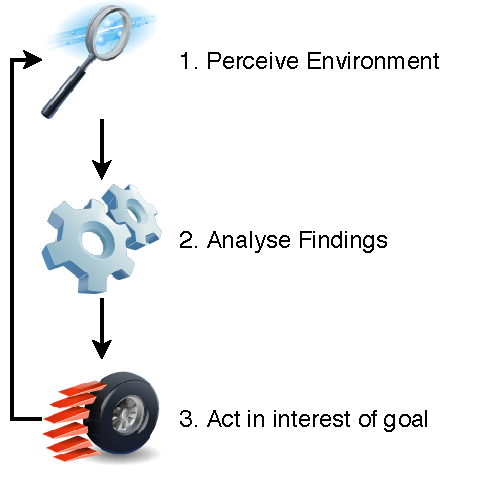
\includegraphics[width = 1\textwidth]{Content/fig/reactive-AI.pdf}
		\caption{Reactive \ac{AI}}
		\label{fig:reactive-ai}
	\end{subfigure}%
	\begin{subfigure}[t]{0.24\textwidth}
		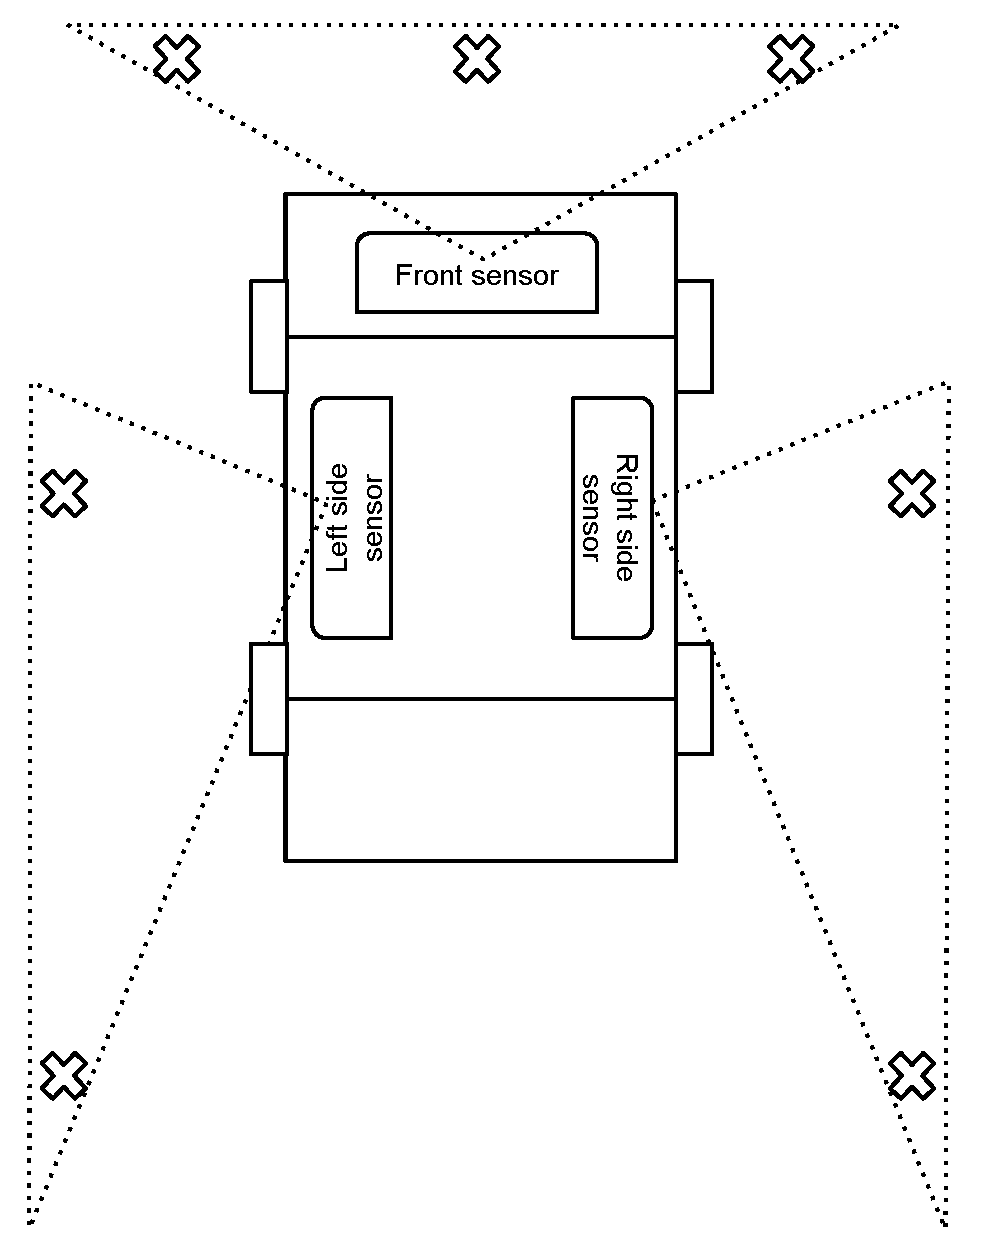
\includegraphics[width = 1\textwidth]{Content/fig/AutoVehicle.pdf}
		\captionsetup{justification=centering}
		\caption{Autonomous Vehicle Sensors}
		\label{fig:av}
	\end{subfigure}
	
	\caption{Reactive \texttt{AI-BRO}}
	\label{fig:reactive-aibro}
\end{figure}

Consider an autonomous vehicle, simplified for pedagogy, as shown in Figure~\ref{fig:av} as our motivating example.
The vehicle uses various sensors  to ``see'' the environment around it, while making \emph{lane changing decisions}. 
The sensor outputs are interpreted in order to make decisions based on the dynamic environment. 
The vehicle uses a number of sensors to detect objects in the environment around it. Based on these, it will decide when it needs to change lane
to the \emph{left} or \emph{right}, to \emph{continue} in the current lane, and when to \emph{stop} if necessary. 
The sensors consist of one frontal sensor and a sensor on each side.
The frontal sensor is simplified to detect three positions in front of the vehicle. The side sensors work similarly to the frontal sensor,
and each "see" two positions on each side of the vehicle. 
%Three \acp{ANN} are needed to analyse the sensor outputs in order to make driving decisions.

\acp{ANN} used in \ac{CPS} applications, such as lane changing, are used for decision making tasks 
needed by the controller. Such tasks operate periodically, being reactive in nature,
as shown in Figure~\ref{fig:reactive-ai}. We start by formalising \acp{SANN} using Definition~\ref{def:sann},
which are introduced by us. 

\begin{definition}
	\label{def:sann}
	A \acf{SANN} operates periodically, where the length of each period is 
	an integral multiple of the \emph{tick length} of a ``logical clock'' that \emph{tick}s. Tick length
	is a constant $\in \, \mathbb{R}^{>0}$.
\end{definition}

The periodic behaviour \acp{SANN}, as defined in Definition~\ref{def:sann}, are ideally implemented using the synchronous 
paradigm~\cite{benveniste2003synchronous} and we will use the Esterel programming language~\cite{berry2000foundations} 
to motivate the design of \acp{SANN}. Synchronous programs execute tick-by-tick and during a tick (also known as reaction) the
environment inputs are sampled, the overall system reaction is performed and finally emission of outputs are made. Thus, a tick encapsulates 
the atomicity of reactions, where inputs can happen only at the start of a tick, preventing race conditions arising due to environment 
non-determinism, which is widely prevalent in event triggered paradigms. A synchronous reaction is often represented as a composition of 
multiple, interacting \emph{threads} exhibiting \emph{logical concurrency}~\cite{benveniste2003synchronous}. 
These are usually \emph{compiled-away} to produce sequential code 
that avoid conventional race conditions widely prevalent in the asynchronous setting. Distributed compilation of threads, which is a much harder problem, over
multicore platforms is also well developed, though less widely used~\cite{yuan2011compiling}. The synchronous approach guarantees
key properties such as \emph{determinism} and \emph{reactivity}, which is ideal for AI-based CPS. This motivates 
our adoption of the this paradigm while designing \acp{SANN}.


%% add AI-BRO code here
\begin{figure}[htb]
	\begin{lstlisting}[caption={Esterel implementation of \texttt{AI-BRO}},label={lst:ai-bro}]
	module ai-bro:
	
	% data handling declarations -- omitted 
	
	% interface declarations
	input start, A, B, R;
	input fr1: integer, fr2: integer, fr3: integer;
	input s1: integer, s2: integer;
	input s3: integer, s4: integer;
	output O: integer;
	
	loop
	[
	await A;
	% run ANN A: interpret frontal scanner data
	present fr1 or fr2 or fr3 then
	call processFrontSensors()(?fr1, ?fr2, ?fr3);
	end present
	||
	await B;
	% run ANN B: interpret side scanner data
	present s1 or s2 or s3 or s4 then
	call processSideSensors()(?s1, ?s2, ?s3, ?s4);
	end present
	];
	
	% run ANN C: decide on best course of action 
	call makeDecision()();
	% fetch output action
	emit O(getAction());
	each R
	
	end module
	\end{lstlisting}
	%\label{fig:ai-bro}
\end{figure}

We have adapted Berry's well known ABRO example in Esterel~\cite{berry2000foundations} to develop our first example of 
\acp{SANN}. Being an adaptation of ABRO, we term our example, the AI-inspired ABRO, as \texttt{AI-BRO}, and present it in Listing~\ref{lst:ai-bro}.
The original ABRO example performs \emph{the emission of \texttt{O} when both inputs \texttt{A} and \texttt{B} 
	have happened. It resets and restarts this behaviour when the input \texttt{R} happens}. In our setting, the input 
\texttt{A} is used to control the processing of the frontal sensor, and the input \texttt{B} is used for the side sensors.
When both inputs have happened, we start the processing of the decision making network, which outputs the 
lane changing decision using the output \texttt{O}. \texttt{R} resets and restarts this behaviour.

The \texttt{AI-BRO} implementation in Esterel is done using an Esterel module called \texttt{ai-bro} shown in Listing~\ref{lst:ai-bro} on line~\#1.
A module is a basic programming unit in Esterel and the interface of the module consists of input and
output \emph{signals}. We have defined input signals \texttt{A, B, R}, which are \emph{pure signals}
i.e. these are Boolean in nature carrying a status --- either \emph{present / true} or \emph{absent / false} during a tick. The output signal 
\texttt{O} is valued and in addition to its status takes a value of type \texttt{integer}. The interface definitions appear in 
lines \#6-10. \ignore{While these defined signals have global scope, Esterel also has \emph{local signals} and \emph{local variables}, although these are not used in this 
	program. }% However, a local variable called \texttt{out} of type \texttt{integer} is defined on line \#10.
A variable, unlike a signal, has no status information. 

The main logic of the program is composed of two concurrent threads (denoted using the \texttt{||} operator)
that await external events \texttt{A, B} to happen. 
This task can be performed concurrently as these two inputs may happen either simultaneously in the same tick or 
in an interleaved manner in different ticks. Upon occurrence of the respective event, corresponding data processing 
is performed by the invocation of the appropriate \ac{ANN}, implemented as the C function \texttt{processFrontSensors()}
and \texttt{processSideSensors()}. Both these functions encapsulate pre-trained neural networks. Thus, when both events have 
happened and both networks have executed, the two concurrent threads are terminated. The two threads are also grouped using the 
grouping operators (denoted by \texttt{[ ]}), which are put in sequence using the sequence operator (denoted by the ``\texttt;''). %,with the statements starting from line \#24. 
Thus the third neural network, called \texttt{makeDecision()},
can trigger only after the data from both the front and side sensors have been processed. 
The output of this decision is subsequently emitted through the valued signal \texttt{O}, on line \#30, which will indicate the chosen lane changing action.

Finally, the main logic is enclosed in a \texttt{loop..each R} construct. This is a \emph{preemption construct} that preempts and restarts the 
loop on every \texttt{R} input, maintaining reactive behaviour with every reset.
This will happen after each lane changing decision.

\ignore{The first \ac{SANN} takes input from the frontal sensor, i.e. it receives three integer inputs (either 1 or -1). 
	This \ac{SANN} the outputs the suggested course of action based off of these inputs: stop, turn left/right or continue.  
	The second \ac{SANN} takes input from both side sensors, i.e. it receives four integer inputs (either 1 or -1). 
	This \ac{SANN} returns a simplified version of whether or not is it safe for the vehicle to move in either direction.
	The last \ac{SANN} takes in the outputs of the first and second \acp{SANN} and decides on the best course of action
	for the vehicle based on those inputs: stop, turn left/right or continue.}

The \texttt{AI-BRO} example illustrates several features of \acp{SANN}. (1) We are able to create \acp{ANN} that trigger periodically (analogous
to \acp{RNN}) and we can control the timing of these invocations, and (2) Within each period, we can precisely synchronise the 
execution of different \acp{ANN} i.e. the sensor processing \acp{ANN} are synchronised with the external inputs 
\texttt{A, B} while the decision making \ac{ANN} is executed immediately after the first two \acp{ANN} have finished. 
To the best of our knowledge, such precise synchronisation mechanisms are lacking in existing literature on \acp{ANN}.
More importantly, a side effect of the Esterel implementation is that the resultant \ac{ANN} compositions are 
either rejected by the compiler as \emph{non-causal} or compiled into a \emph{causal} implementation that is guaranteed to be
\emph{deterministic} and \emph{reactive}~\cite{benveniste2003synchronous}.

\ignore{the running of \acp{SANN} concurrently and consecutively. If signals A and B are high on the same tick, then both sensor \acp{SANN} will run at the same time. The decision \ac{SANN} will always run after both of the sensor \acp{SANN}. Since these are implemented in Esterel, the system remains causal, deterministic, bounded and, most importantly, time predictable. WCET analysis can be run on AIBRO, with results that are well within the acceptable prediction range.}


\ignore{
	\begin{lemma}
		\label{lemma1}
		The AI-ABRO implementation in Listing~\ref{lst:ai-bro} is an instance of \ac{SANN} defined using Definition~\ref{def:sann}.
	\end{lemma}
}

\begin{prop}
	\label{lemma1}
	The AI-ABRO implementation in Listing~\ref{lst:ai-bro} is an instance of \ac{SANN} defined using Definition~\ref{def:sann}.
\end{prop}

\begin{proof}
	The proof of this trivially follows from the fact that this program is compiled to a single \texttt{tick()} function by the 
	Esterel compiler, where the concurrency is compiled away. Thus, during any tick, we can have a combination of neural networks 
	executing that range from just one network to up to three networks. Assuming that we can execute this program with a fixed tick length 
	(elaborated in section~\ref{sec:wcrt}), the overall period of any network is at most 1-tick. 
\end{proof}

\section{Timing Analysis of \acfp{SNN}}
\label{sec:wcrt}

Time in a synchronous program progresses in logical discrete instants called \emph{ticks}. 
In each tick, the environment is first sampled, then computation takes places, and finally the results are emitted.
In order for safety-critical \ac{CPS}, such as our \texttt{AI-BRO}, to be verified, we need to ensure that the time taken for the execution of any given tick is less than their environmental deadlines.
This necessitates the computation of the worst-case tick length via static timing analysis --- also known as \acf{WCRT} analysis~\cite{roop2009tight}.

\ac{WCRT} analysis needs two things: (1) an architectural model of the
underlying processor architecture; and (2) a \acf{CFG}~\cite{wilhelm2008worst}  representation of
binary program execution over the architectural model. The analysis
process then computes the longest path through the \ac{CFG}.
%For any program, static timing analysis involves first the derivation of a \acf{CFG}~\cite{wilhelm2008worst} which captures the possible execution traces.
%Then, the \ac{CFG} must be annotated with the time taken to execute each node, so that a worst-case path can be derived.
While general purpose programs can feature complications which make this process difficult, Esterel is ideally suited to derivation of \acp{CFG} due to inherent features:  (1) all loops in Esterel are bounded, as there is a need for at least one \texttt{pause} statement
within every loop; and (2) compilers ``compile-away'' the logical
concurrency to produce sequential code. However, as can be seen in
Listing~\ref{lst:ai-bro}, 
Esterel programs can also invoke arbitrary C-functions, which may use
features such as function pointers, unbounded loops, and external interrupts. 
To this end, we provide a set of guidelines and \ac{ANN}
implementation libraries in C,
which restrict these features to make each C function call time
analysable. 

%\subsection{Guidelines}
In this paper, we are using the open-source Platin
tool~\cite{compiler:platin:kps15} for \ac{WCRT}
analysis. Consequently, we have to consider some tool-specific
restrictions to avoid the use of generic features in C that are not
suitable for static analysis, such as system calls, function pointers, interrupt-driven flow, or unbounded loops~\cite{RTOSWCET}.
Hence, the restrictions considered in this paper are: (1) all neural
network functions are coded as bounded \texttt{for} loops; (2) all
memory is statically allocated; (3) variable-length array iterator
functions are coded using preprocessor macros; and (4) the final binary is executed `bare-metal', requiring no
RTOS or OS support, thus avoiding scheduling dependencies
that may be difficult to statically analyse.
\ignore{
	\begin{itemize}
		\item All neural network functions are coded as bounded \texttt{for} loops.
		\item All memory is statically allocated.
		\item Variable-length array iterator functions are coded using preprocessor macros.
		\item The final binary is executed `bare-metal', requiring no
		RTOS or OS support, thus avoiding scheduling dependencies
		that may be difficult to statically analyse.
	\end{itemize}
}

Annotating a \ac{CFG} with execution times is no simple task for many architectures.
Enhancements such as out-of-order execution, multi-level caches, and deep pipelines can all cause complications when considering the time taken to execute program code.
For instance, in~\cite{AirplaneWcet}, Ferdinand et. al. demonstrate the difficulties of determining the worst-case time in arguably simple avionics code running on a Motorola ColdFire 5307.
To avoid these complications, we rely on the Patmos~\cite{patmos:ppes2011} architecture, which is a simple RISC pipeline optimised for static timing analysis. 
Here, caches have simple replacement policies, and it also has a time-predictable memory hierarchy.
It relies on an adaptation of the LLVM compiler that targets the Patmos instruction set.
This simplifies the annotation of the nodes of the \ac{CFG} with
timing costs, thus allowing for a straightforward static analysis of any
\ac{SNN}. Consequently, this work is restricted to the single-core
Patmos architecture and does not examine execution of \acp{SNN} on
other platform types, such as Intel processors and GPUs.
%\changed{Consequently, this work is restricted to the single-core Patmos architecture and does not examine execution of \acp{SNN} on other platform types, such as Intel processors or GPUs}.

%The expense of this is program size, and designers can expect slightly increased program memory usage as a result. 

%When it comes to the annotation of these nodes with their execution times, architectural considerations must be taken into account, for instance memory access times and pipelined execution of instructions.


%\subsection{Patmos}


%We then use the open-source academic timing analysis tool called Platin~\cite{compiler:platin:kps15}, to derive our execution times.


\ignore{
	\begin{example}
		Consider the case of our AI-BRO example in Listing~\ref{lst:ai-bro}. 
		We can express this Esterel program using the \ac{CFG} presented in Figure~\ref{fig:cfg-aibro}.
		\begin{figure}
			\centering
			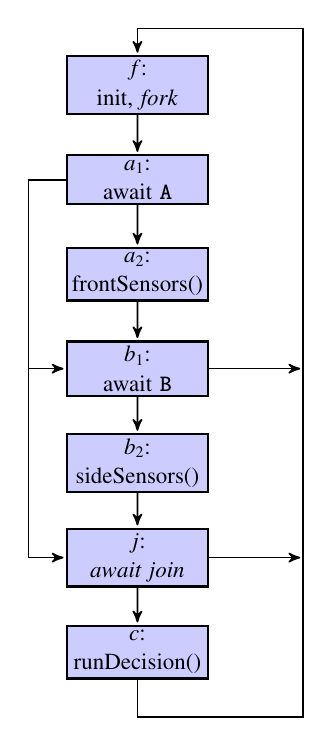
\begin{tikzpicture}[->,>=stealth',shorten >=1pt,auto,
	node distance=2.5cm,
	semithick,scale=0.8, transform shape,scale=0.6, font=\huge]
	
	\tikzstyle{every state}=[rectangle,
	minimum height = 1cm, text width=3.5cm, text centered, 
	fill=blue!20,draw=none,text=black, draw,line width=0.3mm, font=\LARGE]
	
	%start state
	\node[state]
	(init) 
	{$f$: \\init, \textit{fork}}; 
	
	\node[state]
	(awaitA) [below of=init] 
	{$a_1$: \\await \texttt{A}};
	
	\node[state]
	(frontA) [below of=awaitA] 
	{$a_2$: \\frontSensors()};
	
	\node[state]
	(awaitB) [below of=frontA]
	{$b_1$: \\await \texttt{B}};
	
	\node[state]
	(sideB) [below of=awaitB]
	{$b_2$: \\sideSensors()};
	
	\node[state]
	(awaitJoin) [below of=sideB] 
	{$j$: \\ \textit{await join}};
	
	\node[state]
	(decisionC) [below of=awaitJoin] 
	{$c$: \\runDecision()};
	%\node[draw=none]
	%(inv) [below of=init]
	%{};
	
	%\node[draw=none]
	%(inv2) [below of=inv]
	%{};
		
	

	
	\path[->] (init) edge (awaitA);
	\path[->] (awaitA) edge (frontA);
	\path[->] (frontA) edge (awaitB);
	\path[->] (awaitB) edge (sideB);
	\path[->] (sideB) edge (awaitJoin);
	\path[->] (awaitJoin) edge (decisionC);
	
	\draw[->] (decisionC.south) 
		|- ($(decisionC.south) + (0, -1cm)$) 
		-| ($(decisionC.east) + (2.5cm, 0)$) 
		|- ($(init.east) + (0, 1.5cm)$) 
		-| (init.north);
		
	\draw[->] (awaitA.west) 
		-| ($(awaitA.west) + (-1cm, 0)$)
		|- ($(awaitB.west) + (-1cm, 0)$)
		%|- ($(awaitA.160) + (0, 0.75cm)$) 
		|- (awaitB.west);
		
	\draw[->] (awaitA.west) 
		-| ($(awaitA.west) + (-1cm, 0)$)
		|- ($(awaitB.west) + (-1cm, 0)$)
		%|- ($(awaitA.160) + (0, 0.75cm)$) 
		|- (awaitJoin.west);
		
	\draw[->] (awaitB.east) 
		|- ($(awaitB.east) + (2.5cm, 0)$);
		
	\draw[->] (awaitJoin.east) 
	|- ($(awaitJoin.east) + (2.5cm, 0)$);
	
	%\draw[->] (decisionC.south) 
	%	|- ($(decisionC.south) + (0, -1cm)$) 
	%	-| ($(decisionC.east) + (4.5cm, 0)$) 
	%	|- ($(init.east) + (0, 1.5cm)$) 
	%	-| (init.north);
	
	%\draw[->] (awaitA.200) 
	%	|- ($(awaitA.200) + (0, -0.75cm)$) 
	%	-| ($(awaitA.200) + (-2cm, 0)$)
	%	|- ($(awaitA.160) + (0, 0.75cm)$) 
	%	-| (awaitA.160);
		
	%\draw[->] (awaitB.340) 
	%|- ($(awaitB.340) + (0, -0.75cm)$) 
	%-| ($(awaitB.340) + (2cm, 0)$)
	%|- ($(awaitB.20) + (0, 0.75cm)$) 
	%-| (awaitB.20);
	
	%\draw[->] (awaitJoin.195) 
	%|- ($(awaitJoin.195) + (0, -0.75cm)$) 
	%-| ($(awaitJoin.195) + (-1.5cm, 0)$)
	%|- ($(awaitJoin.165) + (0, 0.75cm)$) 
	%-| (awaitJoin.165);
	
	
\end{tikzpicture}

			\caption{Single-thread AI-BRO \ac{CFG}}
			\label{fig:cfg-aibro}
		\end{figure}
	\end{example} \pr{This figure is somewhat non-standard. There are no
		conditional nodes. I suggest you examine the syntax of CFGs
		presented in WCET papers and follow these.}
}

%Fortunately, it is straightforward to convert the synchronous C code generated by Esterel into its equivalent control flow graph.
%Then, as long as the external C function calls that it will call are also predictable, and if the code is run on a time-predictable architecture such as Patmos~\cite{patmos:ppes2011}, the code can be %converted into an equivalent \ac{TCFG}.


%This section discusses the WCRT analysis of SNNs.
%Introduce the WCET problem and then introduce WCRT.
%Intermediate format, timing model, the PATMOS core.
%Coding guidelines for time analysable code. Steps to improve the 
%WCRT. These can be the various subsections.


%When considering normal C code, such as in our external function calls, it can be extremely difficult to construct \ac{CFG}.
%This is because it can be difficult to statically an
%Constructing a \ac{CFG} for a normal general purpose program can be very difficult, especially if it relies on complex software constructs such as system calls, function pointers, interrupts, or unbounded loops.
%This is because the construction of the \ac{CFG} becomes extremely difficult in the face of large branching potentials or unknown jump destinations.


\subsection{\ac{WCRT} algebra}
\label{sec:wcrt-algebra}

Though Esterel is amenable to timing analysis, it still suffers from state space explosion when considering large programs. 
Analysing large sequential code generated from Esterel compilers that ignore \emph{infeasible state space} 
produce large overestimates. \ac{WCRT} algebra, presented in \cite{wang2017timing}, presents a solution to this problem: large synchronous programs can be expressed as 
networks of simpler \ac{TCA}, which have equivalent timing properties to their \ac{TCFG} counterparts. Considering this, we
seek to use this framework to develop a compositional timing semantics of \acp{SNN} and their compositions.

We consider a discrete max-plus structure over
natural numbers $(\Nat_{\infty}, \oplus, \odot, \zero, \one)$ where:
\begin{itemize}
	\item $\Nat_{\infty} \dfs \Nat \cup \{ -\infty, +\infty \}$
	\item  $\oplus$ and $\odot$ are commutative and associate operators that 
	denote the maximum and addition respectively on $\Nat_{\infty}$. 
	\item Neutral elements are $\zero \dfs -\infty$ and $\one \dfs 0$,
	respectively, i.e., $x \oplus \zero = x$ and $x \odot \one = x$. 
\end{itemize}

In particular, $-\infty \odot +\infty = -\infty$. Addition
$\odot$ distributes over max $\oplus$, i.e.,
$x \odot \left(y \oplus z\right) = x + \maxd\left(y, z\right) = \maxd\left(x + y, x + z\right) =
\left(x \odot y\right) \oplus \left(x \odot z\right)$. However, $\oplus$ does not distribute
over $\odot$, for instance, $9 \oplus \left(5 \odot 7\right) = \maxd\left(9, 5 + 7\right) = 12$
while $\left(9 \oplus 5\right) \odot \left(9 \oplus 7\right) = \maxd\left(9, 5\right) + \maxd\left(9, 7\right) = 18$.
This induces on $\Nat_{\infty}$ a (commutative, idempotent) semi-ring.
We denote $\mathcal{W}$ as the set of formulae in this algebra.

We use an automaton called \ac{TCA} to capture the timing behaviour of any \ac{SNN}.
These are mono-cyclic automata, where every state of the automaton is labelled by a
WCRT formula that associates the state with its worst case timing cost.
We start by defining \ac{TCA} using Definition~\ref{def:tca}
%---------------------------------

\begin{definition}
	A \emph{mono-cyclic tick cost automaton}, here after referred to as tick cost automaton (\ac{TCA}) 
	is %a tuple 
	$M = \langle Q, q_0, \rightarrow, \mathcal{W}, L
	\rangle$, where $Q$ is a finite set of \emph{states} with a
	distinguished \emph{entry} state $q_0 \in Q$ and $L: Q \rightarrow \mathcal{W}$ is
	a labeling function that labels every state with its associated timing cost by a formula in $\mathcal{W}$.
	The \emph{transition relation}
	${\rightarrow} \subseteq Q \times Q$ satisfying the following:
	
	\begin{enumerate}
		\item From any state $q_i \in Q$ there is at most one transition to a successor state $q_j \in Q$.
		\item The transitions are such that they form a mono-cycle that starts in $q_0$ and and ends in a 
		transition from some state $q_{n-1} \rightarrow q_0$, resulting in a
		cycle of length $n \in \Nat_{>0}$.
		\item A \ac{TCA} whose cycle length is $1$ is termed
		\emph{mono-periodic}, while those with cycle length $>1$ are called
		\emph{multi-periodic}.
		\item The \emph{reaction time} of a \ac{TCA} is its tick-length, which is
		always fixed to its \ac{WCRT}. 
		\item The \emph{response time} of a \ac{TCA} is the time taken for the
		corresponding \ac{SNN} to produce the outputs given inputs. 
		The response time of a TCA is given by the formula $n \times WCRT$,
		where $n$ is the cycle length.
		%\item The above conditions ensure that a \ac{TCA} is a mono-cyclic automaton.
	\end{enumerate}
	\label{def:tca}
\end{definition}

%---------------------------------
\ignore{
	\pr{Hammond: I have defined both reaction and response time of a
		TCA. We should use these      n our benchmarks, if possible.}
	\begin{example}
		$15 \oplus \left(5 \odot 10\right) = 15$, and $\left(15 \oplus 5\right) \odot \left(15 \oplus 10\right) = 30$.
	\end{example}
	
	\begin{example}
		Consider the program in Listing~\ref{lst:ai-bro}. 
		This had two concurrent threads, which are compiled away to produce sequential code.
		We can express this network's \ac{WCRT} as \\
		$WCRT = \left( a_{await} \odot a_{run} \odot b_{await} \odot b_{run} \odot c_{awaitJoin} \odot c_{run} \odot c_{emit} \right)$, as this is the longest potential path through the system (if we receive both \texttt{A} and \texttt{B} in the same tick).
	\end{example} \pr{Hammond -- since the figure is removed, this formula
		doesn't make any sense now. Please check.}}
%$x \oplus y =$ $MAX(x,y)$ 
%$x \odot y =$ $x + y$ 
\section{Multi-Periodic \acp{SNN} in Esterel}
\label{sec:esterel-mapping}

The mono-periodic implementation of \ac{SNN} using the methodology in Listing~\ref{lst:ai-bro}, while being time predictable, has limitations.
This is because each \ac{NN} must run to completion before any reaction can complete. 
For large networks with many hidden layers, this is not ideal --- as
the overall \ac{WCRT} of the system could become quite large, causing
violations when considering response to some critical inputs which may
need immediate attention to ensure safety. We highlight this aspect
using an \acf{ESS} case study in Section~\ref{sec:results}.

There are other approaches for arranging the internals of each network while still meeting Definition~\ref{def:sann}, and to illustrate this, we will use a simple XOR (exclusive or) \ac{MLP}.
This network is depicted in Figure~\ref{fig:xor-ann}, and as can be seen, it features five neurons in three layers. While we use this simple illustration, the 
methodology is applicable for any \ac{NN}.

\begin{figure}[h]
	\centering
	\scalebox{0.8}{\def\layersep{2.25cm}
\begin{tikzpicture}[shorten >=1pt,->,draw=black!100, node distance=\layersep]
	\tikzstyle{every pin edge}=[<-,shorten <=1pt]
	\tikzstyle{neuron}=[circle,fill=black!25,minimum size=20pt,inner sep=0pt]
	\tikzstyle{input neuron}=[neuron, fill=white!100,draw=black];
	\tikzstyle{output neuron}=[neuron, fill=white!100,draw=black];
	\tikzstyle{hidden neuron}=[neuron, fill=white!100,draw=black];
	\tikzstyle{annot} = [text width=4em, text centered]
	
	% Draw the input layer nodes
	\foreach \name / \y in {1,...,2}
	% This is the same as writing \foreach \name / \y in {1/1,2/2,3/3,4/4}
	\node[input neuron, pin=left:Input $x_\y$] (I-\name) at (0,-\y) {$i_\y$};
	
	% Draw the hidden layer nodes
	\foreach \name / \y in {1,...,3}
	\path[yshift=0.5cm]
	node[hidden neuron] (H-\name) at (\layersep,-\y cm) {$h_\y$};
	
	% Draw the output layer node
	\node[output neuron,pin={[pin edge={->}]right:Output $y$}, right of=H-2] (O1) {$o_1$};
	
	% Connect every node in the input layer with every node in the
	% hidden layer.
	%\foreach \source in {1,...,2}
	%\foreach \dest in {1,...,3}
	%\path (I-\source) edge node[above] {1} (H-\dest);
	\path (I-1) edge node[above] {1} (H-1);
	\path (I-1) edge node[above] {0.5} (H-2);
	\path (I-2) edge node[above] {0.5} (H-2);
	\path (I-2) edge node[above] {1} (H-3);
	
	% Connect every node in the hidden layer with the output layer
	%\foreach \source in {1,...,3}
	\path (H-1) edge node[above] {1} (O1);
	\path (H-2) edge node[above] {-2} (O1);
	\path (H-3) edge node[above] {1} (O1);
	
	% Annotate the layers
	\node[annot,above of=H-1, node distance=2cm] (hl) {\textit{Hidden Layer}\\$l_h$};
	\node[annot,left of=hl] {\textit{Input Layer}\\$l_i$};
	\node[annot,right of=hl] {\textit{Output Layer}\\$l_o$};
\end{tikzpicture}}
	\caption{Example of an XOR \ac{ANN} showing its layers and weights.	\label{fig:xor-ann}}
\end{figure}

Each neuron in this network is based on the model in Figure~\ref{fig:artificial-neuron}, with a simple Boolean step activation function and zero bias. 
The activation function is represented by Equation~\ref{eqn:xor-neuron}, where $y$ is the output, $x \in X$ are the inputs, and $w \in W$ the weights.

\begin{equation}
y =
\begin{cases}
1 & \text{$\Sigma_{i} \left(x_i \times w_i\right) >= 1$} \\
0 & \text{otherwise}
\end{cases}
\label{eqn:xor-neuron}
\end{equation}

\begin{definition}
	\label{def:bb-mlp}
	An \ac{MLP} is formalised as a tuple $M = \langle I, O, N, L,
	\alpha, \eta  \rangle$, where:
	\begin{itemize}
		\item $I$ is a finite collection of input variables with
		its domain being $\mathbf{I} = \mathbb{R}^n$
		\item  $O$ is a finite collection of  output variables with
		its domain being $\mathbf{O} = \mathbb{R}^m$
		\item  $N$ denotes a set of neurons
		\item $L$ denotes a set of layers
		\item $\alpha: N \rightarrow L$ is the neuron mapping function
		that maps a given neuron to a layer
		\item $\eta: \mathbf{I} \rightarrow \mathbf{O}$ is the non-linear
		function (termed the network function) that provides the behaviour of a given network i.e.
		when provided a vector of input of size $n$ produces an
		vector of output of size $m$. Internally, 
	\end{itemize}
	\ignore{
		$i \in I$ is each input to the network, $o \in O$ is each output from the network, 
		$\eta$ is the set of neurons, $L$ is the set of layer functions $l:i \rightarrow o$ which perform intermediate data transforms, $m: \eta \rightarrow L$ is the neuron mapping function that associates a neuron to a given layer,
		and $f: I \rightarrow O$ is a function that captures the non-linear behaviour of the entire network 
		--- i.e. a ``black-box'' untimed non-linear transformation function which converts inputs to outputs via the execution of each layer of neurons in sequence.}
	%$m \subset \eta \times L$ provides the mapping of neurons to layers. 
	%	We can describe the operation of $n$ as $n\left(I\right) = O$, i.e. $n$ describes a `black-box' untimed non-linear transformation function which converts inputs to outputs via the execution of each layer of neurons.
\end{definition} 

\begin{example}
	The \ac{MLP} presented in Figure~\ref{fig:xor-ann} can be presented formally as $I=\langle x_1, x_2 \rangle$, $O = \langle y \rangle$, $N= \{i_1, i_2, h_1, h_2, h_3, o_1\}$ and $L
	= \{l_i, l_h, l_o\}$. The function $\alpha$ maps neurons to
	layers e.g. $\alpha(h_1) = l_1$ and the network function $\eta$
	given input $\langle 0, 1 \rangle$ produces an output $1$
	i.e. $\eta(\langle 0, 1 \rangle) = 1$.
	
\end{example}
%\pr{Illustrate this definition using Figure~\ref{fig:xor-ann}. Also, where is this definition used formally?}

Using Definition~\ref{def:bb-mlp}, we can implement the XOR \ac{ANN} as a ``black-box'' function in Esterel, as presented in Figure~\ref{fig:tca-bb-n}. 
The corresponding mono-periodic \ac{TCA} is shown beside the code.
The \ac{WCRT} is the time taken to execute the network function
$\eta$, i.e. $WCRT\left(M\right) = WCRT\left( \eta\right)$. 
In the following, we use $WCRT(\eta)$ and $\eta$ interchangeably.

\begin{figure}[h]
	\centering
	\begin{subfigure}[h]{0.15\textwidth}
		\centering
		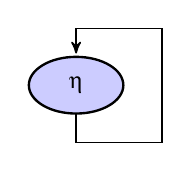
\begin{tikzpicture}[->,>=stealth',shorten >=1pt,auto,
node distance=2.5cm,
semithick,scale=0.8, transform shape,scale=0.6]

\tikzstyle{every state}=[ellipse, minimum width=2.5cm, minimum height=1.5cm, text centered, 
fill=blue!20,draw=none,text=black, draw,line width=0.3mm, font=\LARGE]

%start state
\node[state]
(init) 
{$\eta$}; 

\draw[->] (init.south) 
|- ($(init.south) + (0, -0.75cm)$) 
-| ($(init.east) + (1cm, 0)$) 
|- ($(init.east) + (0, 1.5cm)$) 
-| (init.north);

\end{tikzpicture}

	\end{subfigure}%
	\begin{subfigure}[h]{0.33\textwidth}
		\vspace{3mm}
		\begin{lstlisting}
		loop
		emit y(run_XOR_ANN_n(?x1, ?x2));
		pause;
		end
		\end{lstlisting}
	\end{subfigure}
	\caption{Mono-periodic `black-box' execution, $WCRT = \eta$}
	\label{fig:tca-bb-n}
\end{figure}

It can be noted that by Proposition~\ref{lemma1}, any \ac{ANN} implemented using the approach in Figure~\ref{fig:tca-bb-n} is also an instance of \ac{SNN} defined using Definition~\ref{def:sann}.
%\pr{This is same as the lemma in section 2. Do we need this?}

\begin{theorem}
	\label{thm:bb-soundness}
	(Soundness) A mono-periodic \ac{SNN} given an input vector $\mathbf{i}$
	produces an output vector $\mathbf{o}$ in a given tick \miff the corresponding \ac{MLP} 
	given the same input vector $\mathbf{i}$ produces the identical output vector $\mathbf{o}$ during any execution.
	
	%The synchronous execution of a ``black-box'' function $n$ will give the same output values $O$ for the same input values $I$ as the non-synchronous execution of the
	%\ac{MLP} $n$.
\end{theorem}

\begin{proof}
	The proof of Theorem~\ref{thm:bb-soundness} trivially follows from the
	fact that synchronous execution of a black-box function does not change
	the mathematical properties of that function. %, as all Esterel function
	%calls are state-less and  side effect free.
\end{proof}

\ignore{
	
	\begin{equation}
	y = f\Big(b + \sum_{i=1}^{n} \left(x_i \times w_i\right)\Big)
	\label{eqn:artificial-neuron}
	\end{equation}
	
	In the XOR example, each neuron has a \textit{threshold step function} as its activation function $f$, and has zero bias $b$.
	Hence, each neuron in the \textit{hidden} and \textit{output} layers is following Equation~\ref{eqn:xor-neuron}.
	
	\begin{example}
		In our XOR \ac{ANN}, let $i_1 = 1$ and $i_2 = 0$. \\
		Then, as $1 \times 1 \geqslant 1$, $h_1y = 1$. \\
		However, $\big(\left(1 \times 0.5\right) + \left(0 \times 0.5\right)\big) \ngeqslant 1$, so $h_2y = 0$.
		Likewise, $h_3y = 0$.  \\
		Then, as $\big((1 \times 1) + (0 \times -2) + (1 \times 1)\big) \ngeqslant 1$, the final output $o_1y = 1$.  \\
		This is correct, as $1$ \textit{xor} $0 = 1$.
	\end{example}
}

\begin{figure}[h]
	\centering
	\begin{subfigure}[h]{0.6\textwidth}
		\centering
		\begin{subfigure}[h]{0.3\textwidth}
			\centering
			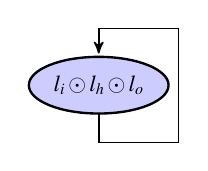
\begin{tikzpicture}[->,>=stealth',shorten >=1pt,auto,
node distance=2.5cm,
semithick,scale=0.8, transform shape,scale=0.6, font=\huge]

\tikzstyle{every state}=[ellipse, minimum width=2cm, minimum height=1.5cm, text centered, 
fill=blue!20,draw=none,text=black, draw,line width=0.3mm, font=\LARGE]

%start state
\node[state]
(init) 
{$l_i \odot l_h \odot l_o$}; 

\draw[->] (init.south) 
|- ($(init.south) + (0, -0.75cm)$) 
-| ($(init.east) + (0.25cm, 0)$) 
|- ($(init.east) + (0, 1.5cm)$) 
-| (init.north);

\end{tikzpicture}

		\end{subfigure}%
		\begin{subfigure}[h]{0.66\textwidth}
			\vspace{3mm}
			\begin{lstlisting}
			loop
			call run_XOR_ANN_li()(?x1, ?x2);
			call run_XOR_ANN_lh();
			emit y(run_XOR_ANN_lo());
			pause;
			end
			\end{lstlisting}
		\end{subfigure}
	\end{subfigure}
\caption{Mono-periodic `layer by layer' execution, $WCRT = l_i \odot l_h \odot l_o$}
\label{fig:tca-bb}
\end{figure}

\begin{figure}[h]	
	\centering
	\vspace{5mm}
	\begin{subfigure}[h]{0.5\textwidth}
		\centering
		\begin{subfigure}[h]{0.3\textwidth}
			\centering
			\begin{tikzpicture}[->,>=stealth',shorten >=1pt,auto,
node distance=2.5cm,
semithick,scale=0.8, transform shape,scale=0.6, font=\huge]

\tikzstyle{every state}=[ellipse, minimum width=2.5cm, minimum height=1.5cm, text centered, 
fill=blue!20,draw=none,text=black, draw,line width=0.3mm, font=\LARGE]

%start state
\node[state]
(l0) 
{$l_i$};

\node[state]
(l1) [below of=l0]
{$l_h$}; 

\node[state]
(l2) [below of=l1]
{$l_o$};  

\path[->] (l0) edge (l1);
\path[->] (l1) edge (l2);

\draw[->] (l2.south) 
|- ($(l2.south) + (0, -0.75cm)$) 
-| ($(l2.east) + (1cm, 0)$) 
|- ($(init.east) + (0, 1.5cm)$) 
-| (init.north);

\end{tikzpicture}

		\end{subfigure}%
		\begin{subfigure}[h]{0.66\textwidth}
			\begin{lstlisting}
			loop
			call run_XOR_ANN_li()(?x1, ?x2);
			pause;
			call run_XOR_ANN_lh();
			pause;
			emit y(run_XOR_ANN_lo());
			pause;
			end
			\end{lstlisting}
		\end{subfigure}
	\end{subfigure}
\caption{Multi-periodic `layer by layer' execution, $WCRT = l_i \oplus l_h \oplus l_o$}
\label{fig:tca-layers}
\end{figure}

\begin{figure}[h]
	\centering
	\vspace{5mm}
	\begin{subfigure}[h]{0.8\textwidth}
		\centering
		\begin{subfigure}[h]{0.3\textwidth}
			\centering
			\begin{tikzpicture}[->,>=stealth',shorten >=1pt,auto,
node distance=2.5cm,
semithick,scale=0.8, transform shape,scale=0.6, font=\huge]

\tikzstyle{every state}=[ellipse, minimum width=2.5cm, minimum height=1.5cm, text centered, 
fill=blue!20,draw=none,text=black, draw,line width=0.3mm, font=\LARGE]

%start state
\node[state]
(l0) 
{$i_1 \odot i_2$};

\node[state]
(l1) [below of=l0]
{$h_1 \odot h_2 \odot h_3$}; 

\node[state]
(l2) [below of=l1]
{$o_1$};  

\path[->] (l0) edge (l1);
\path[->] (l1) edge (l2);

\draw[->] (l2.south) 
|- ($(l2.south) + (0, -0.75cm)$) 
-| ($(l2.east) + (1.5cm, 0)$) 
|- ($(init.east) + (0, 1.5cm)$) 
-| (init.north);

\end{tikzpicture}

		\end{subfigure}%
		\begin{subfigure}[h]{0.66\textwidth}
			\begin{lstlisting}
			loop
			[
			call run_XOR_ANN_i1()(?x1);
			|| 
			call run_XOR_ANN_i2()(?x2);
			];
			pause;
			[
			call run_XOR_ANN_h1()();
			||
			call run_XOR_ANN_h2()();
			||
			call run_XOR_ANN_h3()();
			];
			pause;
			emit y(run_XOR_ANN_o1());
			pause;
			end
			\end{lstlisting}
		\end{subfigure}
	\end{subfigure}
\caption{Multi-periodic, neuron-by-neuron execution, $WCRT = \left(i_1 \odot i_2\right) \oplus \left(h_1 \odot h_2 \odot h_3\right) \oplus o_1$}
\label{fig:tcas-xor}
\end{figure}

As mentioned, using the approach in Figure~\ref{fig:tca-bb-n} to implement complex \acp{ANN} i.e. \acp{CNN} may lead to implementations that violate their timing requirements. 
The synchronous approach, however, enables efficient implementations via compositional modelling.
Esterel supports this via statements such as \texttt{pause} that help to create smaller ticks, \texttt{;} for indicating sequence operation, and \texttt{||}, which enables the modelling of concurrency. 

For example, the \ac{MLP} in Figure~\ref{fig:tca-bb-n} can also be
compositionally modelled by splitting the neural function $\eta$
into its constituent layers $l_i$, $l_h$, and $l_o$. 
While this maintains the overall functionality of the network, it
reduces the \ac{WCRT} by making the network multi-periodic, where each
period is shorter. 
As previously mentioned, the \ac{ESS} case study in Section~\ref{sec:results} examines the benefits of this approach.

%This has no major effect in Figure~\ref{fig:tca-bb}, where the network is still running in a single tick, as function $f$ will call these layers internally anyway.
%However, if \texttt{pause} statements are introduced between each layer, then the timing of the program changes significantly: 
%the \ac{WCRT} of the program will decrease, and the execution becomes `multi-cyclic'.
%Now, multiple \textit{ticks} are required to complete the execution of the neural network, but the program's responsiveness can be increased.

\begin{prop}
	%As long as a neural network's layers are still executed in
	%the correct order, the output will be correct after the last
	%layer is completed.
	The mono-periodic implementation of the XOR \ac{MLP} is functionally
	equivalent to the multi-periodic implementation.
\end{prop}

\begin{proof}
	For any input, output vectors $\mathbf{i, o}$ respectively, 
	$\eta\left(\mathbf{i}\right) = l_o\left(
	l_h\left( l_i\left( \mathbf{i} \right) \right) \right) =
	\mathbf{o}$
	%The proof of this follows intuitively as the operation of $\nu$ already recursively calls each layer $l \in L$ of neurons during execution --- we just remove one layer of indirection.
\end{proof}

\ignore{
	\begin{example}
		In the XOR \ac{MLP}, there are three layers $L = \{l_i, l_h, l_o\}$. 
		During execution, $\eta$ will invoke each layer in order as it executes each neuron. 
		We can make this explicit by calling layers as functions. 
		In this case, $\eta\left(i\right) = l_o\left(
		l_h\left( l_i\left( i \right) \right) \right) = o$
	\end{example} %\pr{While I agree that this result should hold, it is
	%unclear how function composition is actually happening in the
	%code. Code only provides a sequence of function calls without
	%showing the composition!}
}

\ignore{
	For example, a \ac{MLP} $n$ may be compositionally modelled using its constituent layers $l_i$, $l_h$, and $l_o$, as shown in Figure~\ref{fig:tca-bb} (b), (c) and (d).
	\pr{Explain each approach and the trade off. What is the distinction between approach (a) and (b)? Also, could we have just one theorem to 
		state that all approaches are equivalent i.e. they produce the same output albeit in different ticks.}
	
	\begin{lemma}
		A single-tick `layer by layer' execution of functions $l \in L$ the same output as executing function $n$ if all layers are executed in order.
	\end{lemma} 
}




\ignore{
	This has not reduced the \ac{WCRT} of the system, as $n$ has the same \ac{WCRT} as the sum of the three layers that make it up.
	However, if the layers are split over \emph{multiple ticks}, then the system \ac{WCRT} can reduce.
	
	An example of this multi-tick `layer by layer' approach is presented in Figure~\ref{fig:tca-layers}.
	
	\begin{lemma}
		A multi-tick `layer by layer' execution of layers $l \in L \in n$ will give the same output as executing network $n$ completely, iff all layers are executed in order and once a number of ticks equivalent to the number of layers has elapsed. I.e. the number of logical ticks $= |L|$.
	\end{lemma}
	The proof of this is \todo{?}
}

Observe that the response time of the multi-periodic implementation is
$3 \times T_2$, where $T_2$ is the \ac{WCRT} of the multi-periodic
version. In contrast, the response time as well as the reaction time
of the mono-periodic version is always its \ac{WCRT} $T_1$. However, it is
expected that $T_2 << T_1$.
%It is important to note that a multi-tick execution of an \ac{SNN} will not speed up the generation of outputs of the overall network --- as now, multiple ticks must be completed before a given output will be ready. 
%However, the length of each individual tick is reduced, which means that overall the system interactivity can be increased.

Like the breaking up of the function $\eta$ into its component
layers, we can also break each layer $l$ into its component neurons.
This option is presented in Figure~\ref{fig:tcas-xor}. 
Unlike in Figure~\ref{fig:tca-bb}, neurons are able to operate concurrently within each layer. 
This could provide benefits when considering multi-core
implementations such as in \cite{yuan2011compiling}.
\ignore{ however, for single-core single-threaded execution (the focus of this paper), this approach does not considerably alter tick length.} 

A summary of these approaches is presented in Table~\ref{tbl:sann-approaches}.
%we separated each neuron call with \texttt{pause} statements --- i.e. called each neuron in its own tick. 
\begin{table}[h]
	\centering
	\caption{Summary of \ac{SNN} approaches and their relevant figures, \ac{WCRT}, cycles and response time}
	\label{tbl:sann-approaches}
	\begin{tabular}{|l|l|l|l|l|}
		\hline
		Arrangement    & Figures & WCRT & Cycles & Response Time   \\ \hline
		Mono-periodic  & \ref{fig:tca-bb-n},\ref{fig:tca-bb} & High & 1 & == WCRT              \\
		Multi-periodic & \ref{fig:tca-layers},\ref{fig:tcas-xor}& Low  & \textgreater{}1 & \textgreater{}\textgreater{}WCRT \\ \hline
	\end{tabular}
\end{table}


\ignore{ 
	\pr{I suggest we use consistent terminology i.e. mono-cyclic TCA and multi-cyclic TCA and their corresponding Esterel implementation. Ideally, the proof of the theorem 
		can be done using induction. Consider a mono-cyclic implementation and multi-cyclic implementation of length $k$.
		Base case -- first time outputs after 1 tick and k ticks are same. Hypothesis -- outputs after $m$ executions are equivalent i.e. First network executed for 
		$m$ ticks while the second network executed for $k\ times m$ ticks and produced the same output starting from the same input. Proof: to show that this holds for $m+1$ executions.}
}

%\subsection{Implementing `Black-Box' \ac{SNN} in Esterel}

%The basic programming unit in Esterel is a \textit{module}. 
%Each module contains an interface declaration, followed by a body of executable statements.
%Variables are known as \textit{signals}, and may consist of a \textit{status} and a \textit{value} component. 
%Signals with only a status signals are denoted \textit{pure}, while those that contain values are instead denoted \textit{valued}.
%Sections of code may be separated with either the `\code{;}' or `\code{||}' operator, which denote sequencing and synchronous concurrency respectively.
%In order to perform manipulation of valued signals, Esterel can call external functions (provided in supplementary C files).

%Presented in Listing~\ref{lst:blackbox} and Listing~\ref{lst:blackbox-composition} are the simplest way of implementing neural networks in Esterel, already seen in the AI-BRO example.
%As can be seen, entire \acp{ANN} can be composed together and are simply called as external function calls, and will run each tick. 
%Networks can be composed together
%This can be considered the `bare minimum' to qualify as a \ac{SNN}, as the network is now running synchronously with its environment.

%Even though this implementation is quite trivial, it can still gives a strong advantage over a general-purpose implementation: when considering the methodology for composing multiple \acp{ANN}. 
%For example, consider a system that needs three \acp{ANN}, each performing a different task (as is the case in our AI-BRO example, in Section~\ref{sec:motivating-example}). 

%We can compose these multiple \acp{ANN} synchronously in Esterel. 
%As an example of this, consider an extension of our XOR network that computes $y = \big((x_1$ \textit{xor} $x_2)$ \textit{xor} $(x_3$ \textit{xor} $x_4)\big)$ (i.e. $y$ is $true$ when an odd number of inputs are $true$).
%We can compose this together still using the `black-box' methodology, as presented in Listing~\ref{lst:blackbox-composition}.
%Here, it can be seen that the first two \acp{ANN} can be run concurrently with one another, and the third \ac{ANN} can only be run when the first two are complete.



\section{Meta Neural Networks}
\label{sec:concurrent-sann}

%Compared with asychronous implementations, such as C's \texttt{pthread}, it is very simple to create concurrent `parallel' networks in a synchronous system. 
%This is because it is simple to express parallel \acp{ANN} as logically concurrent.
%This logical concurrency will be then compiled away to produce a
%single thread, although, as mentioned in
%Section~\ref{sec:motivating-example}, there are approaches which can
%create truly parallel implementations.

Complex \ac{CPS} use several interacting \acp{NN} to achieve their
functionality. However, to the best of our knowledge, formal modelling
and timing analysis of such concurrent \acp{NN} is lacking. To this
end we propose several alternative architectures, facilitated by the
synchronous approach for formalising the composition and timing of
several interacting \acp{NN}. We term these as \emph{meta neural networks}.
We start by formalising the input-output compatibility requirements.

\begin{definition}
	\label{def:io-compatibility}
	Let $\mathcal{M}$ be a set of \acp{SNN} according to Definition~\ref{def:bb-mlp}.
	We term $M_1 = \langle I_1, O_1, N_1, L_1, \alpha_1, \eta_1 \rangle$, $M_2=\langle I_2, O_2, N_2, L_2, \alpha_2, \eta_2  \rangle$ 
	$\in \mathcal{M}$ input-output compatible,
	IO-compatible for short, when the following hold:
	\begin{itemize}
		\item \emph{Size and type compatibility}: $|I_2|=|O_1|$ and the type of every connection also matches.
		\item \emph{Timing compatibility}: The outputs of $M_1$ are produced in a tick on or before $M_2$
		executes.
	\end{itemize}
\end{definition} 

Hence, just as we are able to break execution of \acp{ANN} over
multiple ticks by calling them 
``layer by layer'', we can also structure the synchronous program such
that it runs a set of concurrent \acp{SNN} ``network by network''.  We term such an arrangement of 
multiple \acp{SNN} as \emph{meta-layers} of \acp{SNN}.

\begin{definition}
	\label{def:nsanns}
	A network of \acp{SNN} organised into meta-layers is a tuple $H = \langle \mathcal{I}, \mathcal{O}, \mathcal{M}, \mathcal{L}, \mathcal{A}, \Delta \rangle$ where:
	\begin{itemize}
		\item We term the first meta-layer as the input
		meta-layer and the last one as the output
		meta-layer.
		\item  $\mathcal{I}=I_1 \cup .. \cup I_k$,
		where $I_1..I_k$ are the inputs of the \acp{SNN} in
		the input meta layer. If $K=|\mathcal{I}|$ then the
		domain is $\mathbf{I} = \mathbb{R}^K$
		\item $\mathcal{O}=O_1 \cup .. \cup O_j$,
		where $O_1..O_j$ are the outputs of the \acp{SNN} in
		the output meta layer. If $J=|\mathcal{O}|$ then the domain is $\mathbf{O} = \mathbb{R}^J$
		\item $\mathcal{M}$ is the set $M \in \mathcal{M}$ of
		\acp{SNN} according to Definition~\ref{def:bb-mlp}
		such any two connected \acp{SNN} are IO-compatible.
		\item $\mathcal{L}$ is the set of meta-layers of \acp{SNN}
		\item $\mathcal{A}: \mathcal{M} \rightarrow \mathcal{L}$ is the network mapping function that maps a given \ac{SNN} to a layer.
		\item $\Delta \subset \mathcal{M} \times \mathcal{M}$ provides the mapping of IO connectivity information between \acp{SNN} of different meta-layers. %@Partha: I am pretty sure we need a place to store the connections between SNNs - no?
	\end{itemize}
\end{definition}

\begin{figure}[H]
	\begin{subfigure}[t]{0.5\textwidth}
		\centering
		\scalebox{0.8}{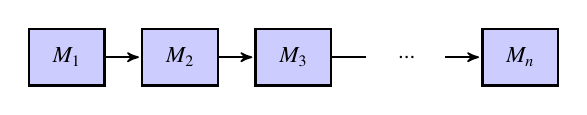
\begin{tikzpicture}[->,>=stealth',shorten >=1pt,auto,
node distance=3cm,
semithick,scale=0.8, transform shape,scale=0.6, font=\LARGE]

\tikzstyle{every state}=[rectangle, minimum width=2cm, minimum height=1.5cm, text centered, 
fill=blue!20,draw=none,text=black, draw,line width=0.3mm, font=\LARGE]

%start state
\node[state]
(n1) 
{$M_1$}; 

\node[state]
(n2) [right of=n1]
{$M_2$};

\node[state]
(n3) [right of=n2]
{$M_3$};

\node[state,fill=none, draw=none]
(el) [right of=n3]
{...};

\node[state]
(nn) [right of=el]
{$M_n$};

\path[->] (n1) edge (n2);
\path[->] (n2) edge (n3);
\path[-] (n3) edge (el);
\path[->] (el) edge (nn);

\end{tikzpicture}
}
		\caption{Pipeline: $WCRT = M_1 \oplus M_2 \oplus M_3 \oplus \ldots \oplus M_n$}
		\label{fig:tca-nn-pipeline}
	\end{subfigure}
	
	\vspace{3mm}
	\begin{subfigure}[t]{0.5\textwidth}
		\centering
		\scalebox{0.8}{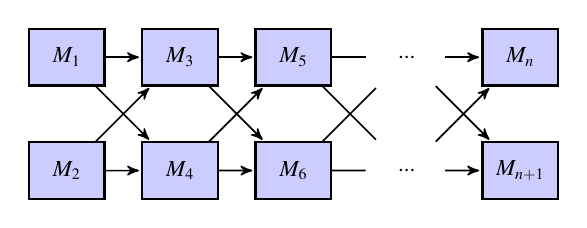
\begin{tikzpicture}[->,>=stealth',shorten >=1pt,auto,
node distance=3cm,
semithick,scale=0.8, transform shape,scale=0.6, font=\LARGE]

\tikzstyle{every state}=[rectangle, minimum width=2cm, minimum height=1.5cm, text centered, 
fill=blue!20,draw=none,text=black, draw,line width=0.3mm, font=\LARGE]

\tikzstyle{every ellips}=[fill=none,text=black,line=none,font=\LARGE]

%start state
\node[state]
(n1)
{$M_1$}; 

\node[state]
(n2) [below of=n1]
{$M_2$};

\node[state]
(n3) [right of=n1]
{$M_3$};

\node[state]
(n4) [right of=n2]
{$M_4$}; 

\node[state]
(n5) [right of=n3]
{$M_5$};

\node[state]
(n6) [right of=n4]
{$M_6$}; 

\node[state,fill=none, draw=none]
(el1) [right of=n5]
{...};

\node[state,fill=none, draw=none]
(el2) [right of=n6]
{...};

\node[state]
(nn) [right of=el1]
{$M_n$};

\node[state]
(nn1) [right of=el2]
{$M_{n+1}$};

\path[->] (n1) edge (n3);
\path[->] (n1) edge (n4);
\path[->] (n2) edge (n3);
\path[->] (n2) edge (n4);
\path[->] (n3) edge (n5);
\path[->] (n3) edge (n6);
\path[->] (n4) edge (n5);
\path[->] (n4) edge (n6);
\path[-] (n5) edge (el1);
\path[-] (n5) edge (el2);
\path[-] (n6) edge (el1);
\path[-] (n6) edge (el2);
\path[->] (el1) edge (nn);
\path[->] (el1) edge (nn1);
\path[->] (el2) edge (nn);
\path[->] (el2) edge (nn1);


\end{tikzpicture}
}
		\caption{Grid: $WCRT = \left(M_1 \odot M_2\right) \oplus \left(M_3 \odot M_4\right) \oplus \ldots \oplus \left(M_n \odot M_{n+1}\right)$}
		\label{fig:tca-nn-grid}
	\end{subfigure}
	
	\vspace{3mm}
	\begin{subfigure}[t]{0.5\textwidth}
		\centering
		\scalebox{0.8}{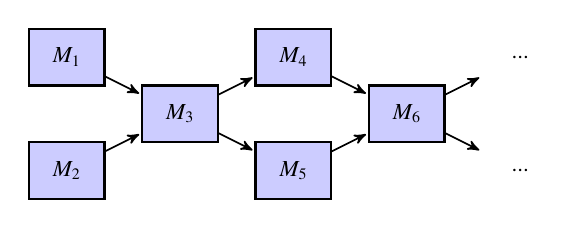
\begin{tikzpicture}[->,>=stealth',shorten >=1pt,auto,
node distance=3cm,
semithick,scale=0.8, transform shape,scale=0.6, font=\LARGE]

\tikzstyle{every state}=[rectangle, minimum width=2cm, minimum height=1.5cm, text centered, 
fill=blue!20,draw=none,text=black, draw,line width=0.3mm, font=\LARGE]

\tikzstyle{every ellips}=[fill=none,text=black,line=none,font=\LARGE]

%start state
\node[state]
(n1)
{$M_1$}; 

\node[state]
(n2) [below of=n1]
{$M_2$};

\node[state]
(n3) [right of=n1, yshift=-1.5cm]
{$M_3$};

\node[state]
(n4) [right of=n3, yshift=1.5cm]
{$M_4$};

\node[state]
(n5) [below of=n4]
{$M_5$};

\node[state]
(n6) [right of=n4, yshift=-1.5cm]
{$M_6$};

\node[state,draw=none,fill=none]
(el1) [right of=n6, yshift=1.5cm]
{...}; 

\node[state,draw=none,fill=none]
(el2) [below of=el1]
{...}; 


\path[->] (n1) edge (n3);
\path[->] (n2) edge (n3);
\path[->] (n3) edge (n4);
\path[->] (n3) edge (n5);
\path[->] (n4) edge (n6);
\path[->] (n5) edge (n6);
\path[->] (n6) edge (el1);
\path[->] (n6) edge (el2);

\end{tikzpicture}
}
		\caption{2x1: $WCRT = \left(M_1 \odot M_2\right) \oplus M_3 \oplus \left(M_4 \odot M_5\right) \oplus M_6 \oplus \ldots$}
		\label{fig:tca-nn-someparallel}
	\end{subfigure}
	
	\caption{Different concurrent \ac{ANN} arrangements}
	\label{fig:tca-nn}
\end{figure}

Depending on the application several options may be explored when
considering the design space for the concurrent arrangement of
multiple networks. Some of these are presented in Figure~\ref{fig:tca-nn}.
The first approach, in Figure~\ref{fig:tca-nn-pipeline}, creates a pipeline of networks, where they are simply executed in sequence.
Alternatively, \acp{SNN} could be arranged in parallel, as in Figure~\ref{fig:tca-nn-grid}. 
Finally, an arrangement might be more arbitrary, as in Figure~\ref{fig:tca-nn-someparallel}. 
Due to the synchronous approach, as long as the \emph{size and type
	compatibility} of Definition~\ref{def:io-compatibility} is
satisfied, it is simple to achieve \emph{timing compatibility} based on Definition~\ref{def:timing-compatibility}. 
Moreover, the worst case timing behaviour of each composition is
straight forward to represent as a formula in \ac{WCRT}-algebra, as
shown in Figure~\ref{fig:tca-nn}.

\begin{definition}
	\label{def:timing-compatibility}
	Timing compatibility between \acp{SNN} in Figure~\ref{fig:tca-nn} may
	be achieved using the following:
	\begin{itemize}
		\item When a \ac{SNN} $M_1$'s output is connected to $M_2$ and the
		period of $M_1$ is $n$-ticks, then for timing compatibility, $M_2$
		has $n$-\texttt{pause} statements at the start.
		\item When a \ac{SNN} $M_1$ and $M_2$'s output is connected to $M_3$ and the
		period of $M_1$ is $n_1$-ticks and that of $M_2$ is $n_2$-ticks,
		then $M_3$ has $(n_1 \oplus n_2)$-\texttt{pause} statements at the start.
		\item When a connectivity self-loop is provided in $\Delta$, we break it explicitly.
	\end{itemize}
\end{definition}

%Contrast this with an asynchronous approach, which could require extensive usage of mutexes and locking mechanisms!

%\subsection{Interfaces of concurrent \acp{SNN}}

\ignore{
	When considering the interconnection of different \ac{SNN} in a network of \ac{SNN} $H$, the connections can only be considered valid iff the source and destination types match, and if the source of an interface is located `earlier' (i.e. on an earlier layer $l \in \mathcal{L}$ or in the global inputs $I$) than the destination interface. 
	More formally, this can be expressed as Definition~\ref{def:sann-conns}.
	
	\begin{definition}
		\label{def:sann-conns}
		A network of \acp{SNN} $H = \langle I, O, \mathcal{M}, \mathcal{L}, \mathcal{A}, \Delta \rangle$ is correctly interconnected iff $\forall \delta \in \Delta, \forall i_d \in I \in n_d \in \delta, \exists i_d \in \left(\mathcal{I} \cup \left(M_s \in \mathcal{M}|\mathcal{A}\left(M_s\right) < \mathcal{A}\left(M_d\right)\right)\right)$, where $i_d$ is the source of connection $\delta$, $M_s$ is the possible source network for the connection, and $M_d$ is the destination network.
		% this should read as:
		% for all connections in H, for all sources of those connections, the source exists in either (an output on a network in an earlier layer that the destination of the connection) or (the inputs I) 
	\end{definition}
}

\begin{figure}[H]
	\centering
	\scalebox{0.8}{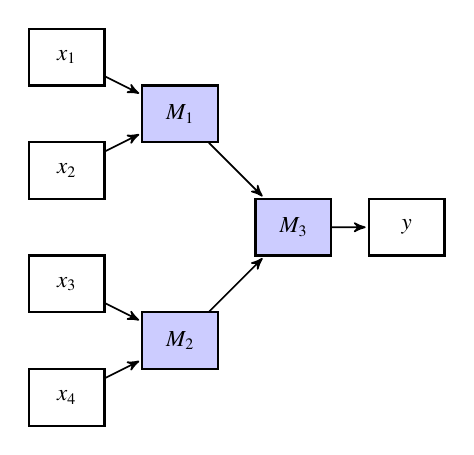
\begin{tikzpicture}[->,>=stealth',shorten >=1pt,auto,
node distance=3cm,
semithick,scale=0.8, transform shape,scale=0.6, font=\huge]

\tikzstyle{every state}=[rectangle, minimum width=2cm, minimum height=1.5cm, text centered, 
fill=blue!20,draw=none,text=black, draw,line width=0.3mm, font=\LARGE]

\tikzstyle{every ellips}=[fill=none,text=black,line=none,font=\LARGE]

%start state
\node[state,fill=none]
(x1)
{$x_1$}; 

\node[state,fill=none]
(x2) [below of=x1]
{$x_2$}; 

\node[state,fill=none]
(x3) [below of=x2]
{$x_3$}; 

\node[state,fill=none]
(x4) [below of=x3]
{$x_4$}; 

\node[state]
(n1) [right of=x1, yshift=-1.5cm]
{$M_1$}; 

\node[state,draw=none,fill=none]
(inv) [below of=n1]
{}; 

\node[state]
(n2) [below of=inv]
{$M_2$};

\node[state]
(n3) [right of=inv]
{$M_3$};

\node[state,fill=none]
(y) [right of=n3]
{$y$};

\path[->] (x1) edge (n1);
\path[->] (x2) edge (n1);
\path[->] (x3) edge (n2);
\path[->] (x4) edge (n2);
\path[->] (n1) edge (n3);
\path[->] (n2) edge (n3);
\path[->] (n3) edge (y);

\end{tikzpicture}
}
	\caption{Simple three-network XOR system}
	\label{fig:three-xor}
\end{figure}

\begin{example}
	\label{ex:simple-xor}
	Consider three XOR \ac{MLP} networks $\mathcal{M} = \left(M_1, M_2, M_3\right)$ in a system $H$.
	They are arranged in the formation shown in Figure~\ref{fig:three-xor}, such that they compute $y = \big(x_1$ \textit{xor} $x_2\big)$ \textit{xor} $\big(x_3$ \textit{xor} $x_4\big)$.
	The overall network $H$ has two meta-layers in $\mathcal{L}$, an input layer and an output layer. 
	Hence, the global inputs $I = \langle x_1, x_2, x_3, x_4 \rangle$, and global outputs $O = \langle y \rangle$.
	The connectivity of $\Delta \in H$ is correctly defined, as the internal connections between $M_1$, $M_2$, and $M_3$ are matching, i.e. they are the same widths and types. 
	
	Let us execute the networks $M \in \mathcal{M}$ using the multi-periodic ``layer by layer'' approach. 
	Hence, for each network $M$, $WCRT = l_i \oplus l_h \oplus l_o$.
	Using \ac{WCRT} algebra, we can compute the system WCRT is of the form $WCRT = \left(M_1 \odot M_2\right) \oplus M_3$, ergo, the actual system \\ $WCRT = \Big(\left(l_1^i \oplus l_1^h \oplus l_1^o\right) \odot \left(l_2^i \oplus l_2^h \oplus l_2^o\right)\Big) \oplus \left(l_3^i \oplus l_3^h \oplus l_3^o\right)$ , where $l^x_y$ indicates layer $l_x \in L_y$ (in network $M_y$).
\end{example}

\ignore{
	Secondly, issues can be caused when considering \emph{alignment} of interconnected networks.
	If two parallel networks take differing numbers of cycles to execute, how can the outputs match cleanly to the inputs of subsequent layers?
	However, this proves to not be a difficult issue to resolve, as tick
	delays can be introduced to parallel networks $n \in l \in
	\mathcal{L}$ such that the number of cycles to execute each network,
	and thus to pass each data variable, is the same.}

The Example in~\ref{ex:timing} discusses the issue of timing compatibility.

\begin{figure}[H]
	\centering
	\scalebox{0.8}{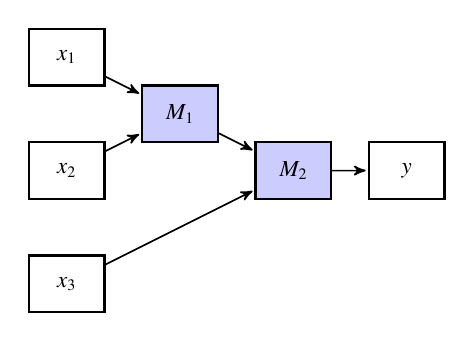
\begin{tikzpicture}[->,>=stealth',shorten >=1pt,auto,
node distance=3cm,
semithick,scale=0.8, transform shape,scale=0.6, font=\LARGE]

\tikzstyle{every state}=[rectangle, minimum width=2cm, minimum height=1.5cm, text centered, 
fill=blue!20,draw=none,text=black, draw,line width=0.3mm, font=\LARGE]

\tikzstyle{every ellips}=[fill=none,text=black,line=none,font=\LARGE]

%start state
\node[state,fill=none]
(x1)
{$x_1$}; 

\node[state,fill=none]
(x2) [below of=x1]
{$x_2$}; 

\node[state,fill=none]
(x3) [below of=x2]
{$x_3$}; 

\node[state]
(n1) [right of=x1, yshift=-1.5cm]
{$M_1$}; 

\node[state]
(n2) [right of=n1, yshift=-1.5cm]
{$M_2$};

\node[state,fill=none]
(y) [right of=n2]
{$y$};

\path[->] (x1) edge (n1);
\path[->] (x2) edge (n1);
\path[->] (x3) edge (n2);
\path[->] (n1) edge (n2);
\path[->] (n2) edge (y);

\end{tikzpicture}
}
	\caption{Two-network XOR system}
	\label{fig:two-xor}
\end{figure}

\begin{example}
	\label{ex:timing}
	Consider the case of a two-input XOR system $H$, as presented in Figure~\ref{fig:two-xor}.
	This will compute $y = \big(x_1$ \textit{xor} $x_2\big)$ \textit{xor} $x_3$.
	As in Example~\ref{ex:simple-xor}, there are two meta-layers in $\mathcal{L}$. 
	Once again, the connectivity of $\Delta$ is correctly defined, as the inputs $I_1 \in M_1$ are simply in the global inputs $I$, and the inputs $I_2 \in M_2$ are provided as both a global input and as the output $O_1 \in M_1$.  
	
	However, as can be seen, the sources for $M_2$ will take different numbers of logical ticks to arrive.
	As a result, we must delay the input $x_3$ by some number of cycles.
	If we are using the multi-periodic ``layer by layer'' execution timing, this number will be $|L \in M_1|$, i.e. the number of ticks it will take to execute the layers of $M_1$ (in our case, $|L| = 3$ cycles). 
	Or, if we are using a mono-periodic black-box approach, then we will need to delay the input $x_3$ by one cycle.
\end{example}

All architectures of meta neural networks discussed thus far are
devoid of instantaneous cycles. While such cycles in asynchronous settings are difficult
to deal with, the synchronous approach offers two different
alternatives. Synchronous compilers can detect such static cycles and flag
them as \emph{non-causal}~\cite{benveniste2003synchronous} programs, and reject them outright. Alternatively, such instantaneous cycles
can be broken by inserting an unit delay (i.e. a \texttt{pause}
statement) to break the cycle.
%\todo{Partha: I don't like the usage of the word "cycle" in here, because we are using mono-cycles and multi-cycles already. Can we use something else?}

%\pr{Hammond -- please read this section and carefully examine the
%  Definitions. Please check that the terminology of your examples and
%  Figures are consistent with my definitions. One question I have
%  about this section is how these are related to the next section.}


%\todo{Discuss how this differs from Asynchronous arragement of ANNs}.
%\todo{Discuss IO with environment. Capture/compute/release, when to capture / release?}

%\todo{Discuss IO compatiblity. Problems: mismatched IO widths, types. Concurrent networks taking different numbers of cycles (sustaining data?)}.



\begin{table*}[h]
	\centering
	\caption{Benchmarks and descriptions}
	\label{table:benchmarks}
	\begin{tabular}{|p{0.1\textwidth}|p{0.06\textwidth}|p{0.16\textwidth}|p{0.4\textwidth}|p{0.08\textwidth}|p{0.11\textwidth}|}
		\toprule
		Name & \ac{ANN} Type                 & Real-time Classification                             & Description                                                   & \#\acp{ANN} & \#Neurons \\ \midrule
		AI-BRO & \ac{MLP}           & Hard real-time                            & The steering controller described in Section~\ref{sec:motivating-example}.                 & 3      & (11, 11, 13)      \\
		ESS & \ac{MLP}   & Hard real-time & Controls an EV charging station with a storage battery. & 3     & (74, 23, 18)      \\
		XOR & \ac{MLP} & Hard real-time                            & Performs Exclusive-Or of two boolean inputs.                 & 1      & 6      \\
		ADDER & \ac{MLP}          & Hard real-time              & Adds two 31-bit numbers together.              & 1      & 5           \\ 
		HELLO & \ac{RNN}     & Hard real-time              & \ac{RNN} trained to remember the letters of `hello'. & 1      & 14      \\
		RABBIT & \ac{MLP}     & Soft real-time              & Turn based, zero-sum game played between two teams of \acp{ANN} & 3      & (50, 60, 60)      \\
		SENSOR & \ac{CNN}     & Soft real-time              & Section~\ref{sec:motivating-example} front sensor implementation for object detection using images. & 1      & 1000+      \\
		\bottomrule
	\end{tabular}
\end{table*}

\section{Case studies and evaluation}
\label{sec:results}
%\pr{I have defined the concept of reaction time and response time. We
%  should have both these in all real-time benchmarks and accordingly
%  evaluate the results.}

We have developed a set of benchmark applications, written in Esterel,
to evaluate the efficacy of the developed approach. These benchmarks are presented in Table~\ref{table:benchmarks}, and are also
publicly available at \textit{https://github.com/PRETgroup/sann}. All benchmarks in this paper were developed in Esterel, C, and where appropriate, Python. 
Hard-real time benchmarks were analysed using the timing analysis tool
Platin~\cite{compiler:platin:kps15}, 
and executed on a Patmos soft-core processor~\cite{patmos:ppes2011} 
on an Altera DE2-115 FPGA running at 50MHz. 
All neural networks were trained offline (i.e. pre-trained).

The benchmarks include an Energy
Storage System (\texttt{ESS}) inspired by~\cite{chaudhari2017hybrid},
the \texttt{AI-BRO} example from Section~\ref{sec:motivating-example}, the \texttt{XOR} network from Section~\ref{sec:esterel-mapping}, and an \texttt{ADDER} developed for
pedagogy. These examples all use \ac{MLP}-based
\acp{SANN}. We have also developed an example involving a \ac{RNN}
called \texttt{HELLO}. 
These first benchmarks are all statically analysed to
compute their \ac{WCRT} and hence could be used in hard real-time
applications. The \texttt{ESS} example is the most complex of these
benchmarks, as it illustrates the concept of meta neural networks
(Section~\ref{sec:concurrent-sann}) involving three neural networks
with 74, 23, 18 neurons respectively.

As this is the first work on synchronous neural networks, we had to
develop time analysable implementations from scratch. Unfortunately, we were unable
to complete the implementation of more complex \acp{ANN} such that they met the requirements of the Platin tool. 
However, we did develop two additional interesting soft-real time examples to illustrate the power of the proposed methodology. The
first example is a computer game called \texttt{RABBIT}, which was
also implemented using Pthreads in Python.
This program demonstrates the
benefits of the synchronous approach. 
Lastly, we developed a \ac{CNN} application called \texttt{SENSOR}, by reusing
libraries from Darknet~\cite{redmon2015real}. This example involved more than 1000 neurons, and we
were able to implement both the ``black box'' and the ``layer by layer'' approaches.

\ignore{
	and have been developed keeping the 
	Two types of \acp{CPS} were considered for this paper: those that are hard-real time, and need their \ac{WCRT} derived, and those that have soft real-time deadlines which can just be measured instead.
	The full suite of these benchmarks are presented in Table~\ref{table:benchmarks}, and are also
	publicly available at \todo{link}. 
	In this section, we discuss these results in more detail.}

%\subsection{Methodology}



%\subsection{An \acf{ESS} System}
\paragraph{An Energy Storage System \texttt{ESS}}
\label{sec:ess}
\acf{ESS} are used to lower the costs of
charging an electric vehicle (EV)~\cite{chaudhari2017hybrid}. %\pr{Please cite the TII journal version.}
Simply put, an \ac{ESS} serves as an intermediary between the electrical grid and a large electrical load i.e. an EV.
Usually, it is made up of a connection to the grid, a connection to
the load, one or more electrical storage devices (such as batteries), and a controller to manage the system, as 
depicted in Figure~\ref{fig:ess-components}.

\begin{figure}[b]
	\vspace{-3mm}
	\centering
	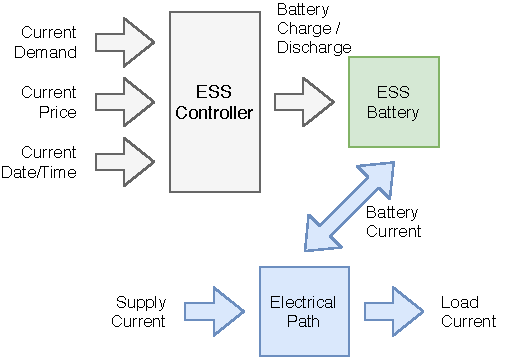
\includegraphics[scale=0.68]{Content/fig/ess_components}
	\caption{Example \ac{ESS} Components\label{fig:ess-components}}
\end{figure}

\acp{ESS} work by shifting the burden of their electrical load to the
electrical grid during periods of low demand, i.e. when the price is the cheapest.
Then, as the load on the grid increases along with consequent increase
in price, the \ac{ESS} starts to supply its load from its battery instead. 
This results in a lower average cost for providing the load current. 
This system must be functionally correct while also meeting timing
deadlines i.e.
the system must respond to safety situations within a time bound. 

Our \texttt{ESS} has an associated
over-current detector.  When this triggers, the system must evade this
unsafe situation within 30 milli-seconds to activate a circuit
breaker, which must take effect within this deadline. 
However, the response time of the overall \texttt{ESS} controller is much less strict, as it has a soft-real time \textit{quality of service} deadline of one second.
This is primarily because the demand input of the \texttt{ESS} does not need to be sampled faster than every second for suitable behaviour.
In addition, the price of electricity changes only once every 10 minutes.
%  \pr{You may also
%  add the response time requirement upfront, which is from input to
%  the corresponding output of a given \ac{SANN}.}

\ignore{Deciding when to charge and discharge an \ac{ESS} battery is non-trivial. 
	There are many factors to consider, including the current \ac{SoC} of the battery, historical data on pricing and load demand current.
	A variety of approaches have been used, including statistical modelling in \cite{TOUESS}.
	%In addition, a system that is in charge of a battery must include
	%safety features, i.e. an electrical over-current detector, to ensure
	%that the users of the \ac{ESS} remain safe at all times: In the event
	%of an over-current, the industry standard requires that this unsafe
	%situation should be evaded within 30ms. 
}

We propose a meta neural network, involving three 3-layer \ac{MLP} \acp{SANN}, to decide when to charge and discharge the battery in our \texttt{ESS}.
These networks operate synchronously with a over-current detector
that preempts the system by activating a circuit breaker.
The architecture of this meta neural network is presented in Figure~\ref{fig:ess-sanns}. 
%In this case, 
%Using the ``layer by layer'' approach, we can guarantee a low \ac{WCRT} to ensure safety in the face of an electrical over-current, 
%as the \textit{Safety Cutoff} heuristic will be evaluated in each synchronous tick.

\begin{figure}
	\centering
	\scalebox{0.7}{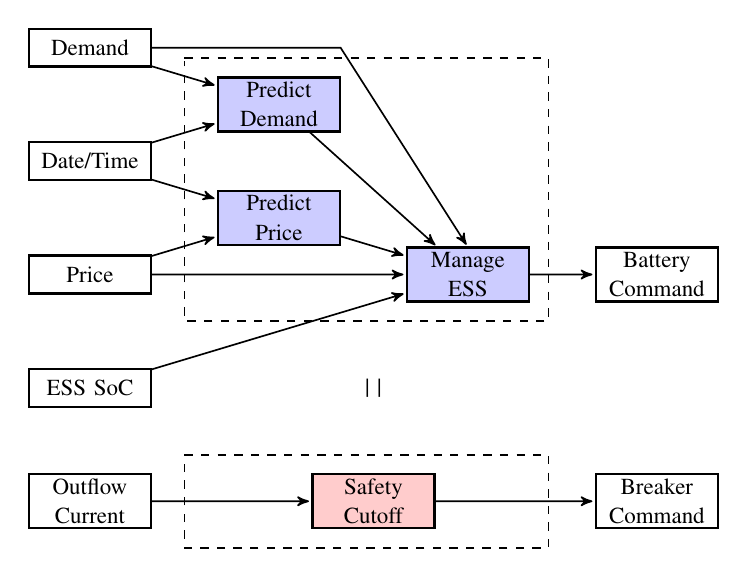
\begin{tikzpicture}[->,>=stealth',shorten >=1pt,auto,
node distance=3cm,
semithick,scale=0.8, transform shape,scale=0.6, font=\huge]

\tikzstyle{every state}=[rectangle, text width=3cm, minimum height=1cm, text centered, 
fill=blue!20,draw=none,text=black, draw,line width=0.3mm, font=\LARGE]

%start state
\node[state,fill=none]
(cdemand)
{Demand}; 

\node[state,fill=none]
(ctime) [below of=cdemand]
{Date/Time};

\node[state,fill=none]
(cprice) [below of=ctime]
{Price}; 

\node[state,fill=none]
(csoc) [below of=cprice]
{ESS SoC}; 

\node[state,fill=none]
(ccur) [below of=csoc]
{Outflow Current}; 

\node[state]
(prdemand) [right of=cdemand, xshift=2cm, yshift=-1.5cm]
{Predict Demand}; 

\node[state]
(prprice) [below of=prdemand]
{Predict Price}; 

\node[state]
(ess) [right of=prprice, xshift=2cm, yshift=-1.5cm]
{Manage ESS};

\node[state,fill=red!20]
(scut) [right of=ccur, xshift=4.5cm]
{Safety Cutoff}; 

\node[state,draw=none, fill=none]
(parallel) [above of=scut]
{\texttt{||}}; 

\node[state,fill=none]
(essoutp) [right of=ess, xshift=2cm]
{Battery Command};

\node[state,fill=none]
(breaker) [right of=scut, xshift=4.5cm]
{Breaker Command};

\path[->] (cdemand) edge (prdemand);
\path[->] (ctime) edge (prdemand);
\path[->] (ctime) edge (prprice);
\path[->] (cprice) edge (prprice);
\path[->] (cprice) edge (ess);
\path[->] (prdemand) edge (ess);
\path[->] (prprice) edge (ess);
\path[->] (csoc) edge (ess);
\path[->] (ess) edge (essoutp);
\path[->] (ccur) edge (scut);
\path[->] (scut) edge (breaker);

\draw[->] (cdemand.east)  
	|- ($(cdemand.east) + (5cm, 0)$) 
	-\ (ess.north);
	
\draw[-,dashed] ($(prdemand.north) + (-2.5cm, 0.5cm)$) 
-| ($(ess.east) + (0.5cm, 0)$) 
|- ($(ess.south) + (0, -0.5cm)$)
-| ($(prdemand.north) + (-2.5cm, 0.5cm)$);

\draw[-,dashed] ($(scut.north) + (-5cm, 0.5cm)$) 
-| ($(scut.east) + (3cm, 0)$) 
|- ($(scut.south) + (0, -0.5cm)$)
-| ($(scut.north) + (-5cm, 0.5cm)$);

\end{tikzpicture}
}
	\caption{ESS \ac{SANN} / Safety Cutoff arrangement}
	\label{fig:ess-sanns}
\end{figure}

Training this system complex, as it is not
feasible to provide all possible correct commands for every possible
input. Hence, back-propagation could not be used.
Instead, Q-learning~\cite{qlearning2010}, a type of reinforcement learning, was used for training the network.
\ignore{ Reinforcement learning trains an \ac{ANN} without knowledge of the
	correct output. 
	
	It trains based on the reinforcement of the reward of any given action $A$, with regard to the current state $S$. 
	An action that is \emph{good} will be given a high reward, and the \ac{SANN} will get its weights updated in an attempt to preserve the behaviour.
	A \emph{bad} action, however, will result in the  weights being modified so that it will have a reduced chance of choosing that action in that state again. 
	Using this system, Q-learning attempts to train an \ac{SANN} to follow the path of highest reward.}


%In our case, demand and price were modelled as sine functions, and the networks were trained with the goal of reducing the overall ``real-world'' cost \pr{I don't understand what you mean here?}
%of outputting energy from the \ac{ESS} system. 
%The \ac{ESS} was rewarded for buying energy when it was cheap, and supplying it when it was expensive.

In order to validate this design, we performed \ac{WCRT} analysis of
both the mono-periodic and multi-periodic implementations. 
%\pr{What
%  was the length of the multi period? For all these benchmarks, we
%  have to state the length of the period and the how many cycles are
%  needed. In particular, we have to state from input to output how
%  long it takes for all approaches.}
These results are presented in Table~\ref{tbl:res-ess}.

\begin{table}[H]
	\centering
	\caption{\ac{WCRT} results for \texttt{ESS}}
	\label{tbl:res-ess}
	\begin{tabular}{|l|l|l|}
		\hline
		Approach         & WCRT (ms) & Response Time (ms)\\ \hline
		Black-box        & 14   & 14 \\ 
		Layer by layer   & 9.8  & 58.8 \\ \hline
	\end{tabular}
\end{table}

As can be seen, the \ac{WCRT} for the mono-periodic ``black-box''
approach is $14ms$, 
making the total worst-case cut-off time $28ms$ (one cycle to capture value, one cycle to emit command).
This only gives $2ms$ for the hardware to respond to a digital signal
to cut the circuit, which may not be sufficient.

Considering this, we developed  a multi-cyclic ``layer by layer''
approach, that results in a \ac{WCRT} of $9.8ms$, 
giving a total worst-case cut-off time time of $<20ms$. 
This gives sufficient time for the physical hardware to respond and break the circuit.
In addition, although changing the implementation to multi-cyclic does increase the \ac{ANN} response time by $54.8$ms, it does not
come close to the deadline of the \ac{ESS} battery command, which has a one second soft-real time deadline.

\paragraph{\texttt{AI-BRO}}
%\subsection{AI-BRO} 
Introduced in Section~\ref{sec:motivating-example}, and as depicted in Figure~\ref{fig:av}, \texttt{AI-BRO} uses three different \acp{SANN} working together to guide an automatic vehicle. 
For this case study, the \acp{SANN} were simple \acp{MLP}.
Each was trained using back-propagation with a gradient descent approach~\cite{yegnanarayana1994artificial}, as the correct outputs for each of the inputs could be exactly specified.
For instance, \texttt{AI-BRO}, a front sensor reading of $(010)_2$ implies an obstacle directly in front of the vehicle.
Therefore, the vehicle must either turn left, turn right, or stop.
%\changed{\sout{The front \ac{SANN} is responsible for passing this information to the driver \ac{SANN}.}}
Consequently, it should output $(101)_2$.
%The first network takes input from the frontal sensors. These consist of 3 boolean values.
%Then, it outputs an initial suggestion for the car to travel, as an enumerated value across 3 bits for 6 different actions \textit{\{stop, stop/turn left, stop/turn right, turn left, turn right, continue straight\}}.

%Like the first network, the second \ac{SANN} also processes sensor data. 
%This time, the inputs are boolean values coming from the side sensors.
%A single boolean output for each side indicates whether or not a given direction is obstructed.

%The third and final \ac{SANN} takes in the outputs from the two sensor-processing networks. 
%Using the information they provide, it makes the actual decision for the car to follow.


Once created, \ac{WCRT} values were able to be derived for both mono-cyclic and multi-cyclic implementations, and are provided in Table~\ref{tbl:res-aibro}.

\begin{table}[H]
	\centering
	\caption{\ac{WCRT} results for \texttt{AI-BRO}}
	\label{tbl:res-aibro}
	\begin{tabular}{|l|l|l|}
		\hline
		Approach         & WCRT (ms) & Response Time (ms)\\ \hline
		Black-box        & 2.8  & 2.8  \\ 
		Layer by layer   & 1.9  & 11.4 \\ 
		Neuron by neuron & 1.8  & 10.8 \\ \hline
	\end{tabular}
\end{table}


\paragraph{\texttt{XOR} / \texttt{ADDER}}
%\subsection{XOR / ADDER}
\label{sec:xor-and-adder}

In addition to the exclusive-or \ac{MLP} \texttt{XOR} used as an example in Sections
\ref{sec:esterel-mapping} and \ref{sec:concurrent-sann},
an \ac{MLP} \texttt{ADDER} was also created that could add two 31-bit numbers together. 
These two networks were both straightforward to train and analyse 
due to their simple 3-layer designs, and their \acp{WCRT} are presented in Table~\ref{tbl:res-xor-adder}.

\begin{table}[H]
	\centering
	\caption{\ac{WCRT} results for \texttt{XOR} and \texttt{ADDER}}
	\label{tbl:res-xor-adder}
	\begin{tabular}{|l|l|l|}
		\hline
		Approach         & WCRT (ms) & Response Time (ms)\\ \hline
		\multicolumn{3}{|l|}{\texttt{XOR}}  \\ \hline
		Black-box        & 0.82 & 0.82   \\ 
		Layer by layer   & 0.57 & 1.71  \\ 
		Neuron by neuron & 0.6  & 1.8 \\  \hline
		\multicolumn{3}{|l|}{\texttt{ADDER}}  \\ \hline
		Black-box        & 0.49 & 0.49   \\ 
		Layer by layer   & 0.39 & 1.17  \\ 
		Neuron by neuron & 0.33 & 0.99 \\  \hline
	\end{tabular}
\end{table}

\paragraph{\texttt{HELLO}}
%\subsection{HELLO}

The \texttt{HELLO} system is a 3-layer \ac{RNN} which was trained to learn the pattern of the word ``hello''. 
We implemented this system to demonstrate that the synchronous
approach works with any type of \acp{ANN}, not just \acp{MLP}.
The results of this system are presented in Table~\ref{tbl:res-hello}.

\begin{table}[H]
	\centering
	\caption{\ac{WCRT} results for \texttt{HELLO}}
	\label{tbl:res-hello}
	\begin{tabular}{|l|l|l|}
		\hline
		Approach         & WCRT (ms) & Response Time (ms)\\ \hline
		Black-box        & 2.22  & 2.22  \\ 
		Layer by layer   & 1.33  & 3.99  \\ \hline
	\end{tabular}
\end{table}


\paragraph{\texttt{RABBIT} and \texttt{SENSOR}}
%\subsection{RABBIT}

%\pr{Is this a well known game? Citation needed}.


\ignore{The game is played in turns between two teams: wolves and a rabbit who
	are moving in a map. The wolves play on the same turn, working
	together to catch the rabbit. 
	The rabbit plays alone and attempts to escape the map. The wolves play on the same turn, working together to
	catch the rabbit. The rabbit scores if it leaves the map before time
	runs out. The wolves, on the other hand, win if they catch the
	rabbit before time runs out. The game runs in a loop. At the
	start of every round, all animals decide \textit{at the same time}
	where they will move too. 
	The system then updates and computes the score accordingly. Unless
	there was a winner, or time ran out, the 
	iterations continue.}

The \texttt{RABBIT} game was designed to highlight the benefits of synchronous
programming while designing meta neural networks. 
The game is played in turns between two teams, wolves and a rabbit, who
are moving in a map.
Each animal in the game has its own functional \ac{ANN}, which operate synchronously, respecting causality and avoiding deadlocks. 
The same system was also implemented in Python (using
Pthreads), without the use of any synchronization primitives, and we found
that the %\changed{\sout{
%We used
%these examples to evaluate the correlation coefficient between the
%Python and the Esterel implementation and found that the }
outputs of the two versions were
strongly correlated. %}

\ignore{The \acp{ANN} were run concurrently on separate Pthreads and the system updated after each \ac{ANN} thread finished running. 
	Although uncommon, it was noted that the Pthread implementation was
	susceptible to producing scores that should have been impossible
	for the system to attain. For example, the rabbits and wolves scoring on the same turn; this should not be possible, as either the wolves win or the rabbit, but not both. This was due to the disregard for causality in the
	running of Python's threads. \pr{I am unclear what you are claiming
		here. What is an impossible score and why? Are you referring to
		typical race conditions?}
	
	%Unfortunately this system is not currently time analysable using Platin. The system was originally implemented without regard to the timing analysis guidelines of \acp{SANN} as listed in Section~\ref{sec:wcrt}. As a result, this system contains some code that prevents WCET analysis at this time.
	
	Due to the large number of neurons in the \acp{ANN} of this system, one of the wolf \ac{ANN} was used to calculate the correlation coefficient between an Esterel implementation of an \ac{ANN}, i.e. \ac{SANN}, and an asynchronous \ac{ANN} using the exact same weights.
	
	The results of these calculations are presented in Table~\ref{tbl:res-game}.
	\begin{table}[H]
		\centering
		\caption{Correlation coefficient results for \texttt{RABBIT}}
		\label{tbl:res-game}
		\begin{tabular}{|l|l|}
			\hline
			Coefficient & Value \\
			\hline
			Pearson & 0.999999802345 \\
			\hline
		\end{tabular}
	\end{table}
	
	\paragraph{SENSOR}
	%\subsection{SENSOR}
}


\acp{DNN} have many industrial applications compared to any other type
of \ac{ANN}. This is largely due to their ability to train to
extremely large amounts of data. We implemented a \texttt{SENSOR}
application using a \ac{DNN}. An open source library called Darknet~\cite{redmon2015real} was used
to implement this \ac{CNN}. Darknet provides a platform for training
of many types of \acp{ANN} in C, including \acp{CNN}. 
%\changed{\sout{Using an already trained \ac{CNN} that can perform object recognition
%on input images, an Esterel system was created to run this \ac{CNN}, using the
%mentioned blackbox approach and the layer--by--layer approach.}
Using this system, an Esterel application was developed to recognize images using the black-box and the layer by layer approaches.%}

\begin{table}[H]
	\centering
	\caption{MNN2C Static \ac{WCRT} results for \texttt{ESS}, \texttt{AI-BRO}, \texttt{XOR} and \texttt{ADDER}}
	\label{tbl:res-mnn2c}
	\begin{tabular}{|p{0.15\textwidth}|p{0.15\textwidth}|p{0.15\textwidth}|p{0.15\textwidth}|p{0.15\textwidth}|p{0.15\textwidth}|}
		\hline
		Benchmark         & Original Black-box WCRT (ms) & MNN2C Black-box WCRT (ms)  &  \% decrease & MNN2C Multicore WCRT (ms) & \% decrease\\ \hline
		\texttt{ESS}        & 14 & 4.41 & 68.5 & 2.43 & 82.64 \\  \hline
		\texttt{AI-BRO}        & 2.8 & 2.29 & 18.21 & 1.47 & 47.5 \\ \hline
		\texttt{XOR}        & 0.82 & 0.53 & 35.37 & 0.53 & 35.37 \\  \hline
		\texttt{ADDER}        & 0.49 & 0.37 & 24.49 & 0.37 & 24.49 \\ \hline
	\end{tabular}
\end{table}

\begin{table}[H]
	\centering
	\caption{Combined \ac{WCRT} results for \texttt{ESS}, \texttt{AI-BRO}, \texttt{XOR}, \texttt{ADDER} and \texttt{HELLO}}
	\label{tbl:res-sann}
	\begin{tabular}{|l|l|l|l|}
		\hline
		Approach         & WCRT (ms) & Response Time (ms) & Size (neurons) \\ \hline
		\multicolumn{4}{|l|}{\texttt{ESS}} \\ \hline
		Black-box        & 14  & 14 & 125 \\ 
		Layer by layer   & 9.8  & 58.8 & 125 \\
		MNN2C			 & 4.41 & 4.41 & 125 \\ \hline
		\multicolumn{4}{|l|}{\texttt{AI-BRO}}  \\ \hline
		Black-box        & 2.8  & 2.8 & 35 \\ 
		Layer by layer   & 1.9  & 11.4 & 35 \\ 
		Neuron by neuron & 1.8  & 10.8 & 35 \\ 
		MNN2C			 & 2.29 & 2.29 & 35 \\ \hline
		\multicolumn{4}{|l|}{\texttt{XOR}}  \\ \hline
		Black-box        & 0.82 & 0.82 & 6  \\ 
		Layer by layer   & 0.57 & 1.71 & 6 \\ 
		Neuron by neuron & 0.6  & 1.8 & 6 \\ 
		MNN2C			 & 0.53 & 0.53 & 6 \\ \hline
		\multicolumn{4}{|l|}{\texttt{ADDER}}  \\ \hline
		Black-box        & 0.49 & 0.49 & 5  \\ 
		Layer by layer   & 0.39 & 1.17 & 5 \\ 
		Neuron by neuron & 0.33 & 0.99 & 5 \\ 
		MNN2C			 & 0.37 & 0.37 & 5 \\ \hline
		\multicolumn{4}{|l|}{\texttt{HELLO}}  \\ \hline
		Black-box        & 2.22  & 2.22 & 14 \\ 
		Layer by layer   & 1.33  & 3.99 & 14 \\ \hline
	\end{tabular}
\end{table}

\ignore{
	\pr{How
		many layers? Can we give some measurement-based timing analysis
		results for the game and the CNN?}
	The system ran through 16 layers, taking approximately 500ms for all 16 layers to run. This time was taken by measurement and is not a WCET value. Although no WCET analysis was possible, due to the open source library not following any of the timing analysis guidelines listed in Section~\ref{sec:wcrt}, the system was able to run in Esterel. This shows that the synchronous implementation of \acp{DNN} using C and Esterel is not only possible, but that the whole range of \acp{ANN} can be implemented synchronously using the Esterel programming language.
}














\section{\acf{MNN2C}}
\label{sec:mnn2c}
\acfp{MBD} is a traditional approach to designing systems~\cite{dmd2019}.
As opposed to design by trial-and-error, \ac{MBD} builds formally defined, safer systems~\cite{dmd2019}.
This approach to creating systems is highly preferred where the safety of the system, e.g. systems that interact with humans, is concerned.
This is relevance where \ac{AI} systems are created that interact with the same environment as humans, such as the \acf{ESS} shown in Section~\ref{sec:ess}.

The ability to generate formally defined system models from existing \acp{ANN} allows for potentially unsafe and unpredictable \acp{ANN} to be re-implemented in such a way that they are safe and predictable.
This allows the use of such \acp{ANN} in systems were safety is critical, e.g. \acf{CPS}.

Keras~\cite{chollet2015keras} is an \ac{ANN} Python library, able to use TensorFlow as a backend. 
Keras enables the quick, easy and highly adaptable training of various \acp{ANN}.
The \acp{ANN} generated by Keras are not safe: they are not formally defined, and any timing must be done using measurement based timing. 
This poses a problem to the use of the \acp{ANN} in \ac{CPS}, since \ac{CPS} have strict rules and protocols that the software must follow.

\acf{MNN2C} is an \ac{ANN} compiler that aims to produce \acf{MNN} models in C using pre-existing, Keras-trained \acp{ANN}.
The C code that \ac{MNN2C} produces is not only time-predictable, but the generated \acp{MNN} are also formally defined in \ref{def:snn}.
This means that the \ac{MNN} models generated can be used in \ac{CPS} with the knowledge that these \acp{MNN} are rigorously, mathematically defined. 
Additionally, \ac{MNN2C} allows for the simple, easy and quick training of \acp{ANN} which can then be implemented in existing C systems.

\subsection{Results}
The software generated by \ac{MNN2C} was not only highly accurate, with a correlation coefficient of 1.0 compared to the original Keras generated \ac{ANN}, but also had a lower static \ac{WCET} compared to the code originally created in this chapter.
Using the built-in \ac{WCET} compiler, the timing results were easily found for each time-predictable example from Table~\ref{tbl:res-sann} and are shown in Table~\ref{tbl:res-mnn2c}.
This table shows that the structure of the \ac{MNN} being analysed has a large influence on the timing properties of that \ac{ANN}. 
The \ac{ESS} \ac{MNN}, which has a lot fewer non-linear activation functions (using a lot of Re-Lu activations compared to Tanh) has a much larger decrease in \ac{WCET} compared to the other benchmarks, which average a 26\% decrease.
This shows that the \acp{MNN} generated by \ac{MNN2C} better manage the implementation of the activation functions it uses, giving more accurate \ac{WCET} of the \ac{MNN}.

\begin{table}[H]
	\centering
	\caption{MNN2C Static \ac{WCRT} results for \texttt{ESS}, \texttt{AI-BRO}, \texttt{XOR} and \texttt{ADDER}}
	\label{tbl:res-mnn2c}
	\begin{tabular}{|p{0.2\textwidth}|p{0.2\textwidth}|p{0.2\textwidth}|p{0.2\textwidth}|}
		\hline
		Benchmark         & Original Black-box WCRT (ms) & MNN2C Black-box WCRT (ms)  &  \% \textbf{decrease} \\ \hline
		\texttt{ESS}        & 14 & 4.41 & 68.5 \\  \hline
		\texttt{AI-BRO}        & 2.8 & 2.29 & 18.21 \\ \hline
		\texttt{XOR}        & 0.82 & 0.53 & 35.37 \\  \hline
		\texttt{ADDER}        & 0.49 & 0.37 & 24.49 \\ \hline
	\end{tabular}
\end{table}

\subsection{Future Work}
\ac{MNN2C} currently only generates time predictable, formally defined C code \acp{ANN} based off of Keras \acp{ANN}.
While this is a huge step, this is not the limit when it comes to using \acp{ANN}.
\ac{MNN2C} can be expanded to generate code that is implementable on various hardware platforms, such as \acp{FPGA}, graphics cards and many others.
This would allow for the implementation of \acp{ANN} in various \ac{CPS} besides those that just use C software.








\section{Summary}
This chapter introduced the concept of \acfp{SNN} and their timing properties.

In Section~\ref{sec:motivating-example}, \acp{SNN} and their behaviour are introduced. 
Additionally, a motivating example is given with it's Esterel implementation.

Section~\ref{sec:wcrt} introduces the methods by which timing analysis is done on \acp{SNN} and the algebra involved with this.
This chapter also gives the first formal definition of a \ac{SNN} and discusses the periodicity of these \acp{SNN}.

The next section, Section~\ref{sec:concurrent-sann}, introduces the concept of \acfp{MNN} and provides formal definitions for them, as well as providing examples of the structure of the introduces \acp{MNN}.

A new Python compiler for creating \acp{MNN} from Keras is introduced in Section~\ref{sec:mnn2c} and its results are presented.

The final section of this chapter presents the results of the work done on \acp{SNN} and \acp{MNN} for this chapter.
These results are discussed and analysed, with conclusions drawn in the following chapter.

\section{Discussion}
\label{sec:conclusion}

In this work, we have presented an approach for synchronous composition of \acf{RE} with \acfp{ANN} for \acp{CPS} by defining \acfp{SNN}.
Our \acp{SNN} demonstrate that policies specifying safe I/O behaviours for \acp{ANN} can be enforced.
These enforced policies are shown to increase the safety and efficiency of the systems within which they are placed, without adding a large overhead to the system and without decreasing the functionality of the system.
In the three case studies presented, the \ac{RE} added an average overhead of just 6.035\%, but the efficiency and safety of each system was increased by an amount that rendered the overhead negligible.






\chapter{Runtime Enforcement of Synchronous Neural Networks}

\section{\acf{CPS}}
\acf{CPS} refer to a network of distributed controllers that manage the physical processes of the system~\cite{cps-design}~\cite{alur2015principles}. 
\ac{CPS} encompass a wide variety of disciplines, from mechatronics to civil infrastructure (Figure~\ref{fig:cps}).
\ac{CPS} operate in the physical world, where environments can be unpredictable and uncontrolled.
This introduces safety concerns for the \ac{CPS}; the hardware must be predictable and reliable, and the software must be predictable and reliable.
This thesis focuses on the software requirements for \ac{CPS}.

\begin{figure}[h]
	\centering
	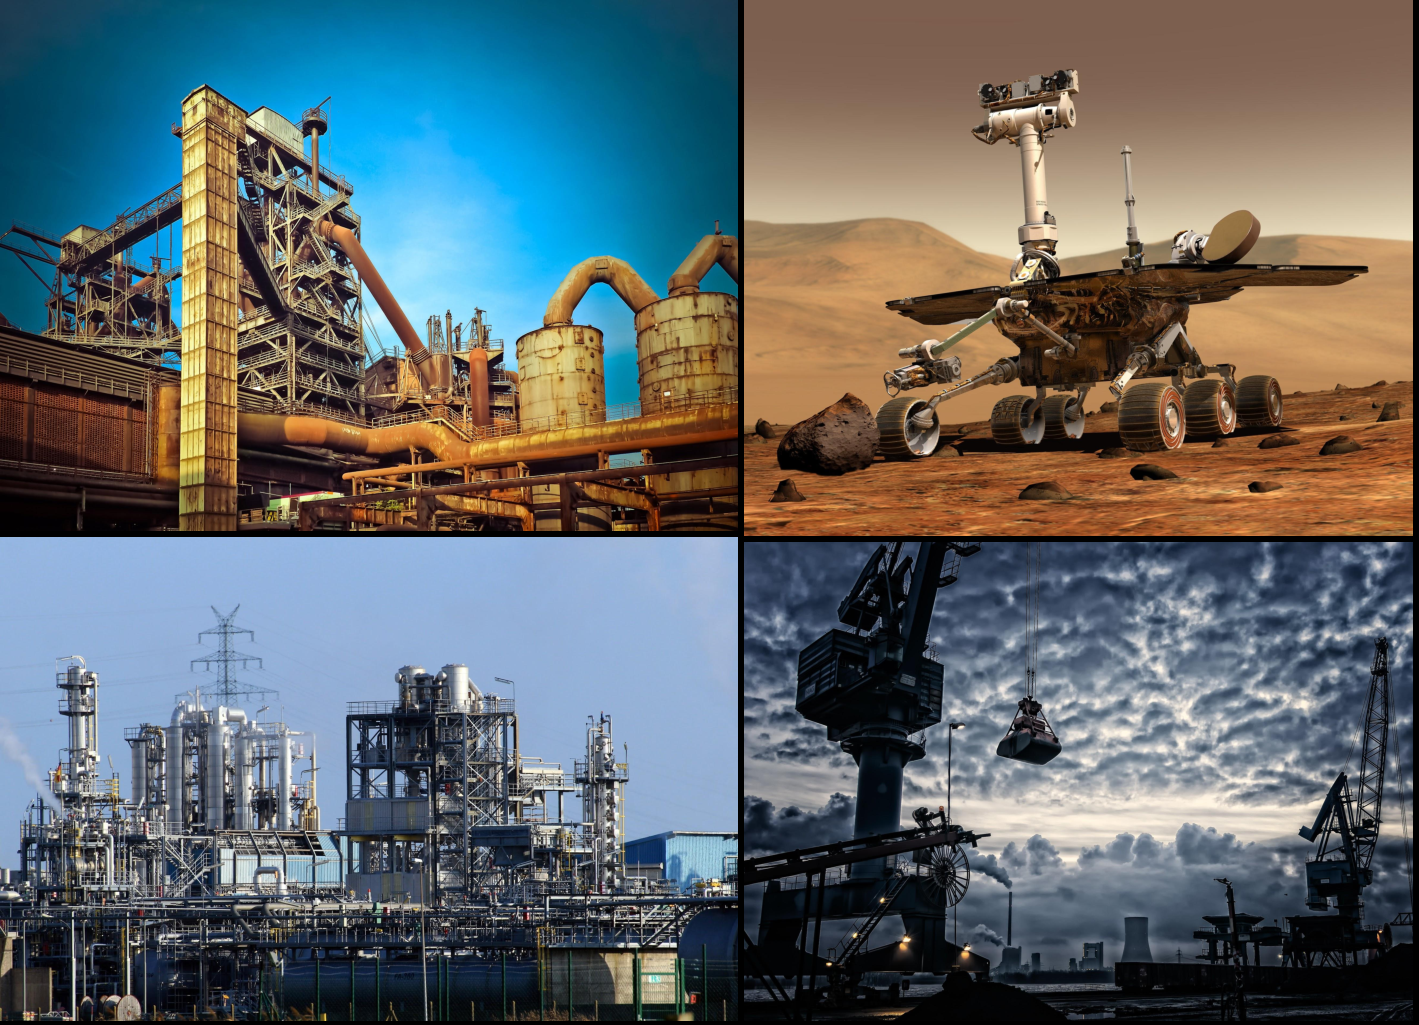
\includegraphics[width=\textwidth]{Content/fig/1234.pdf}
	\caption{Examples of \ac{CPS}~\cite{industry-pic}~\cite{crane-pic}~\cite{rover-pic}~\cite{factory-pic}, from left to right, top to bottom: A) factories, B) robotics, C) power and electricity, and D) construction \label{fig:cps}}
\end{figure}

\ac{CPS} applications encompass real-time systems, where the systems need to satisfy a set of timing and functional requirements to ensure correct operation. 
Here, a missed deadline may result in catastrophic consequences, making these \ac{CPS} highly \textit{safety-critical}. 
These have strict timing and functionality requirements --- any errors in control can result in physical damage, injuries, and/or fatalities~\cite{ANNDevModel1999}. 


\section{\acf{AI} and \acf{ML}}
\acf{ML} is a field of data science where \acfp{AI} are taught to learn large and/or complex data relationships~\cite{ai}.
\ac{AI} come in many shapes and forms, from decision trees to \acfp{ANN}~\cite{ai-types}.
\ac{AI} were invented to fill a gap that humans cannot, where they can store a huge number of data relationships and learn new relationships where a person would struggle.
\ac{AI} are used all over industry, from industrial systems, to cybernetics and robotics (such as Figure~\ref{fig:ai-girl}).

\begin{figure}[h]
	\centering
	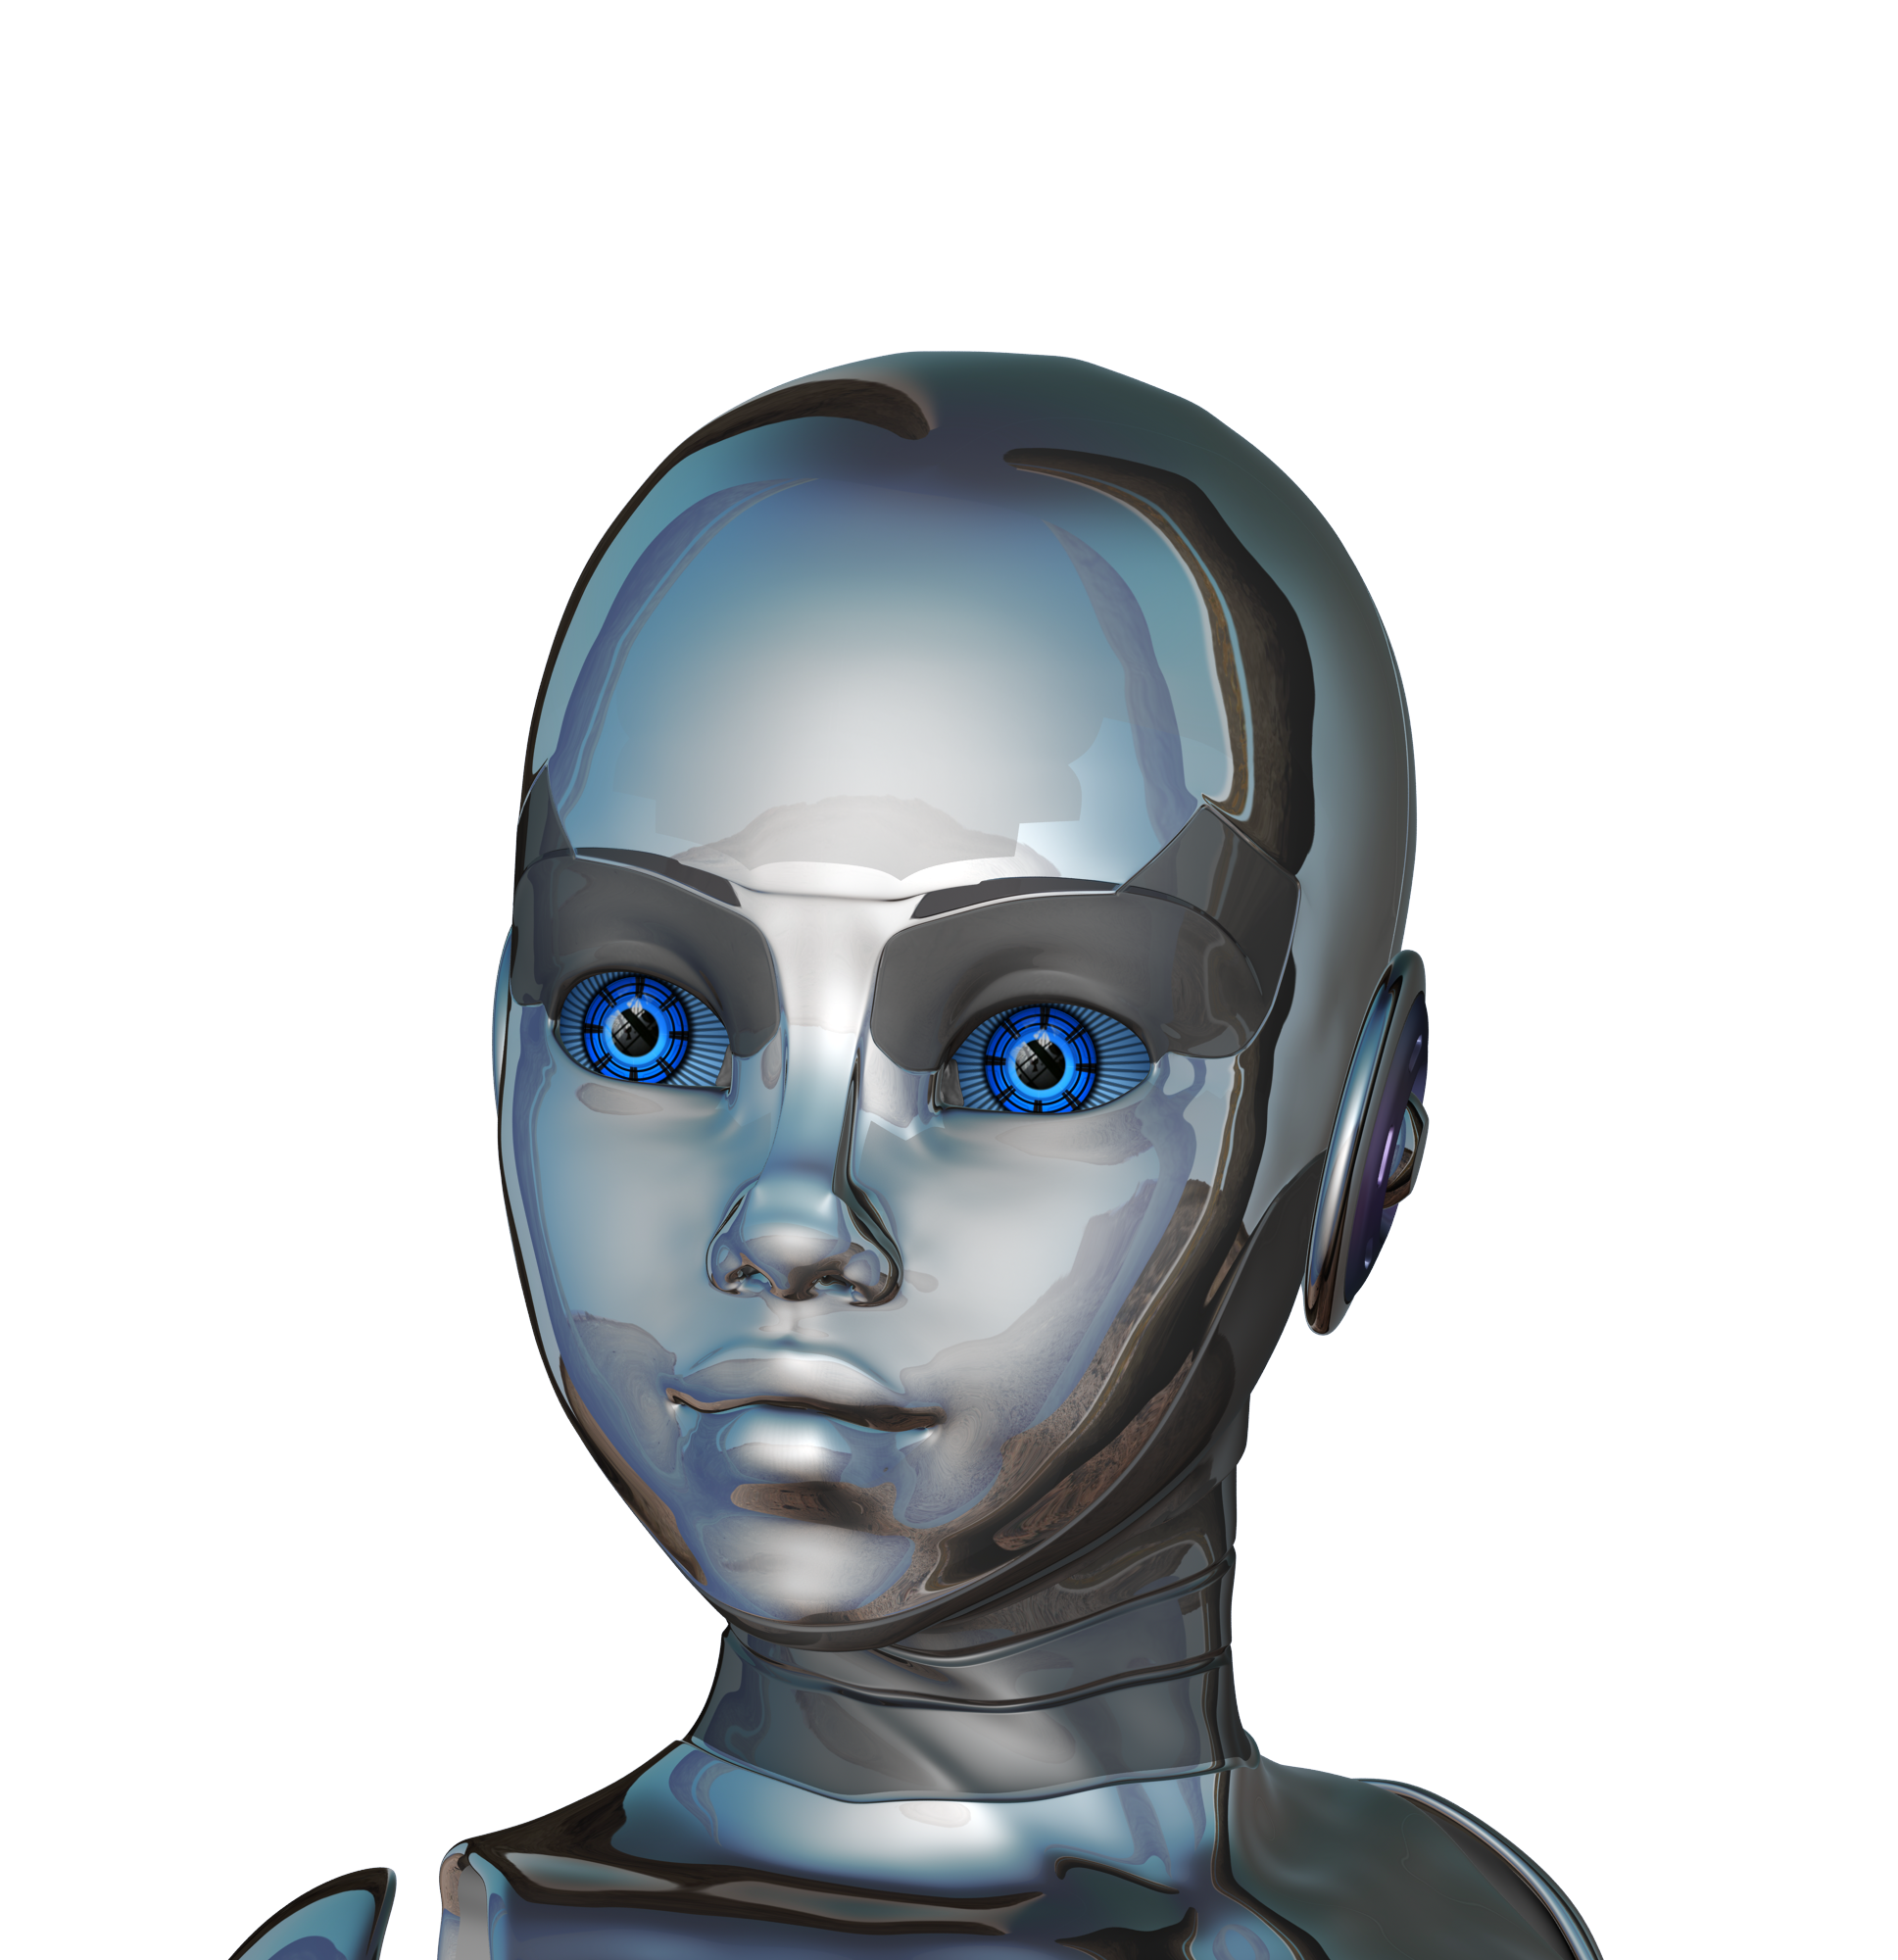
\includegraphics[width=0.4\textwidth]{Content/fig/ai-girl.png}
	\caption{\acp{AI} are frequently used as the controllers of robots~\cite{robotgirl-pic} \label{fig:ai-girl}}
\end{figure}

\ac{AI} are increasingly used in \ac{CPS}, where safety is critical.
However, the mathematical nature of \ac{AI} is non-linear, leaving many \ac{AI} difficult to verify and validate.
Additionally, as \ac{AI} adapt to learn larger data sets and more complex relationships, the size and complexity of the \acp{AI} increase.
Some of these \acp{AI} are easier to verify and validate than others~\cite{aiverify} however, as they grow in size, these techniques take more time and other resources to implement.
In \ac{CPS}, it is essential for all components to be verified and validated, and thus the issue with \ac{AI} in \ac{CPS} is made clear: conventional techniques cannot be used to verify \acp{AI} for \ac{CPS}.

\subsection{\acfp{ANN}}
\acp{ANN} are a type of \ac{AI} designed to model the functionality of the human brain~\cite{kohonen1988introduction}.
The resulting \acp{ANN} are generally large and complex.
They are composed of layers interconnected artificial neurons, each neuron passing numerical messages along to the next, and can be represented mathematically by a complex, non-linear equation.
They are able to store large and complex data relationships~\cite{ANNSafety2007}, like their biological counterpart, and this is where they are most useful.
However, the result is that \acp{ANN} are extremely difficult to verify or validate~\cite{menzies2005verification}.

\acp{ANN} are often used in big data and Internet of Things (IoT), but also show up in \ac{CPS} such as \acfp{AV}.
Their use in \ac{CPS} is highly contended, as \acp{ANN} are not 100\% reliable and accidents happen~\cite{coldewey_2018}.
Thus, it is of utmost importance that any \ac{ANN} used in any \ac{CPS} is verified to be safe for that system in all possible environments.
Without that guarantee of safety the use of \ac{AI} in such systems is risky and an endangerment to any person involved with the system and its environment~\cite{ANNSafety2018}.
There exists a large body of research dealing with the safety of \acp{ANN}, but there are plenty of opportunities for research towards safe \acp{ANN}.

\section{Contribution}
This thesis provides novel techniques to the verification and validation of \acfp{ANN} in \acf{CPS}.
There is a large body of work regarding the safety of \acp{ANN}, ranging across a whole variety of applications and approaches.
However, no work has been done regarding the synchronous implementation of \acp{ANN} and the verification available to synchronous \acp{ANN}, which we term \acfp{SNN}.  
This thesis addresses the issue of safe \acp{ANN} using synchronous semantics~\cite{berry1991}.

In this thesis, a new \ac{ANN} library was created to demonstrate the benefits of synchronous \acp{ANN}.
In the benchmarks using deep \acp{ANN}, an existing library called Darknet~\cite{darknet13} was used to implement the deep \acp{ANN}.
However, a tool chain was created to replace Darknet that compiles Keras~\cite{chollet2015keras} trained \acp{ANN} to the created \ac{ANN} library.

The major contributions of this thesis are as follows:
\begin{itemize}
	\item A time predictable approach to \acp{ANN} is developed using the synchronous language Esterel~\cite{berry2000foundations}. These predictable \acp{ANN} are termed \acfp{SNN} and are defined using formal methods. Using T-CREST's Patmos processor architecture~\cite{patmos:ppes2011}, timing analysis of these \acp{SNN} is possible. These \acp{SNN} provide a safe approach to implementing \acp{ANN} in \ac{CPS}. The results of the \acp{SNN} are presented using a set of benchmarks. 
	\item \acfp{MNN} are proposed as a framework for the composition of multiple \acp{SNN}. The thesis provides formal definitions for the \acp{MNN} and benchmarks are presented that show their efficacy. 
	\item The combination of \acf{RE} and \acp{SNN} is investigated, with the intent to modify unsafe events. This provides functional safety for \acp{SNN}, something not covered in previous chapters. An \acf{AV} case study is introduced for the purposes of this work and a simulation is created to demonstrate its efficacy.
	\item \acf{RV} of \acp{MNN} is proposed as an approach to dealing with input perturbation. This demonstrates a functional verification method for \acp{ANN} that have complex inputs, such as image classification \acfp{CNN}, where \ac{RE} is not an option. An \ac{AV} case study is also created for this work, with an \ac{AV} object detection simulation created to demonstrate the benefits of this proposition. 
\end{itemize}

\section{Thesis Structure}
This chapter, Chapter 1, introduces the problem statement, provides some background to the problem and then introduces the approach this work takes to address the problem.

Chapter 2 gives a basic understanding of the concepts required to understand this research towards safe \acp{ANN} for \ac{CPS}.

Chapter 3 introduces the concept of \acfp{SNN} and their timing properties.
Formal definitions of \acp{SNN} and their related components are provided in Chapter 3.
Furthermore, the meta combinations of these \acp{SNN}, termed \acp{MNN}, and the usefulness of such \acp{MNN} in \ac{CPS} is discussed.
Lastly, a new Python tool chain that creates these \acp{SNN} from Keras is also introduced.

Chapter 4 introduces the concept of \acf{RE} in combination with \acp{SNN}. 
This chapter provides formal definitions for the enforcers and the safety policies that are enforced.
An \acf{AV} case study is made for this chapter to show the efficacy of the \ac{RE} of \acp{SNN}.

Chapter 5 proposes two different methods, used in tandem, to increase the safety of systems with complex inputs, such as object detection for \acp{AV}.
The first method is the use of \acp{MNN} to increase the classification accuracy of \acp{SNN}.
The second expands on Chapter 4, and introduces the use of \ac{RV} to increase the safety of \ac{CPS} where \ac{RE} cannot do so.
An \ac{AV} object detection simulation is created as a complex \ac{MNN} and input perturbation is introduced to the system.
The previous approach to \ac{RE} cannot be used, and as such, \ac{RV} is used to functionally verify this system.

Finally, conclusions are drawn on the synchronous approach proposed in this thesis to creating safe \acp{ANN}.


\section{Introduction}
\label{sec:intro2}

\acp{CPS} can be thought of as distributed networks of digital controllers that manage physical processes~\cite{alur2015principles}. 
These have strict timing and functionality requirements --- any errors in control can result in physical damage, injuries, and/or fatalities~\cite{ANNDevModel1999}. 
In the previous chapter we looked at the timing analysis of \acp{ANN}, this chapter addresses the functional requirements of \acp{ANN}.

\acp{ANN} are being increasingly used as controllers in \ac{CPS} due to their ability to learn data relationships in ways that are difficult to replicate~\cite{ANNSafety2007}. 
\acp{ANN} can deal with novel inputs to the system and are able to outperform other forms of \ac{AI} at computational efficiency, pattern recognition, function approximation and image identification~\cite{AIComp2016, AIComp2017}. 
However, it can be very difficult to ensure the safety of a system involving \acp{ANN}~\cite{ANNSafety2007, ANNSafety2018}.
%As a result, \acp{ANN} should be restricted to advisory roles in \ac{CPS}, due to the difficulty in proving the safety arguments of the \acp{ANN}.% i.e. robustness, \ac{WCET}, accuracy, etc.
%meaning they may not be able to be used to their full capabilities.

This is a concern for systems that are \textit{safety-critical}, as even though it is well-known that \acp{ANN} can be thoroughly trained and produce confidence intervals greater than 90~\%, any misbehaviour in a safety-critical system can result in  catastrophic consequences.
In order for an \ac{ANN} to be used in any capacity within such a system, it should undergo rigorous and thorough validation, verification, and testing procedures to ensure that they it is sufficiently safe for its target system~\cite{scann, ANNSafetyLifecycle2003}.
In order to have \textit{safe} \acp{ANN}, some key problems to consider are: \acp{ANN} must (1) tolerate faults and inconsistencies in their inputs, (2) not create hazardous outputs, (3) be robust and repeatable, and (4) be trained on clean, reliable data~\cite{EstSafeCriteria2003}.

To solve these problems, there exist safety measures such as risk management systems that span the entire development process of the \ac{ANN}~\cite{ANNDevModel1999} and standards with which \acp{ANN} can be certified before they are used in \acp{CPS}~\cite{SCANNStandard}, producing \acp{ANN} that are classified as \textit{safe enough} for their role. 
However, as \acp{ANN} become larger and more full-featured, they  become harder to statically analyse.
Problematic situations can arise when an \ac{ANN} exhibits unexpected behaviour that the system is unable to safely respond to.

To address this issue, we propose the use of \ac{RE} within the \ac{ANN} domain for \ac{CPS} as a methodology for protecting the safety of \ac{CPS} \textit{at runtime}.
\ac{RE} is an existing approach to ensuring the safety of \acp{CPS} and is used to enforce safety policies that monitor and edit the events of the target system~\cite{rta-cps}.
\ac{RE} is formally defined to be used in \acp{CPS}~\cite{recps}, however there has been no formal approach to combining \ac{RE} with \acp{ANN}. 

% What is in this paper
The key contributions of this chapter are thus: (1) we propose combing \acp{SANN} and \ac{RE} for the first time; (2) we provide formalisation for \ac{RE} by formally defining \acfp{VDTA} and (3) we show that this synchronous composition results in a system that is safe, i.e. it produces safe outputs and responds to real-time deadlines. 


\section{Related Work}
\label{sec:related}


%More recently, progress has been made in the field of verification of Deep \acp{ANN}. 
Verification of \ac{ANN}, specifically, \acfp{DNN}, can be performed for properties (such as robustness and accuracy) using \ac{SMT}~\cite{Gehr2018AI2SA,reluplex,DeepANNverify}. 
Using \ac{SMT} and other techniques, certain safety properties of an \ac{ANN}, such as robustness, can be demonstrated. 
This is useful, because the robustness of a deep \ac{ANN} is a critical to its safety.
A robust \ac{ANN} is one that will provide consistently accurate outputs even when the input to the \ac{ANN} is noisy, incorrectly coloured or otherwise distorted. 
However, \ac{SMT} has issues with scale: as the \acp{ANN} to analyse become larger, analysis time grows exponentially~\cite{Gehr2018AI2SA}, making it very difficult to verify large, deep \acp{ANN}.
%Ergo, they are less efficient on larger deep \acp{ANN}.
In addition, they require the deep \acp{ANN} to meet a set of design constraints, requiring specific activation functions and limiting the \ac{ANN} architectures.
For instance in \cite{Gehr2018AI2SA}, where the robustness of \acfp{CNN} is verified by using an abstract technique, only \acp{CNN} and \acp{MLP} \acp{ANN} with the \ac{ReLU} activation functions can be statically analysed.
This limits flexibility, as each \ac{ANN} must be designed around these restrictions. % thus limiting properties of the \ac{ANN}, such as its activation function and size, could result in an \ac{ANN} that is inefficient, not robust, slow, etc.

 







\section{Multi-Periodic \acp{SNN} in Esterel}
\label{sec:esterel-mapping}

The mono-periodic implementation of \ac{SNN} using the methodology in Listing~\ref{lst:ai-bro}, while being time predictable, has limitations.
This is because each \ac{NN} must run to completion before any reaction can complete. 
For large networks with many hidden layers, this is not ideal --- as
the overall \ac{WCRT} of the system could become quite large, causing
violations when considering response to some critical inputs which may
need immediate attention to ensure safety. We highlight this aspect
using an \acf{ESS} case study in Section~\ref{sec:results}.

There are other approaches for arranging the internals of each network while still meeting Definition~\ref{def:sann}, and to illustrate this, we will use a simple XOR (exclusive or) \ac{MLP}.
This network is depicted in Figure~\ref{fig:xor-ann}, and as can be seen, it features five neurons in three layers. While we use this simple illustration, the 
methodology is applicable for any \ac{NN}.

\begin{figure}[h]
	\centering
	\scalebox{0.8}{\def\layersep{2.25cm}
\begin{tikzpicture}[shorten >=1pt,->,draw=black!100, node distance=\layersep]
	\tikzstyle{every pin edge}=[<-,shorten <=1pt]
	\tikzstyle{neuron}=[circle,fill=black!25,minimum size=20pt,inner sep=0pt]
	\tikzstyle{input neuron}=[neuron, fill=white!100,draw=black];
	\tikzstyle{output neuron}=[neuron, fill=white!100,draw=black];
	\tikzstyle{hidden neuron}=[neuron, fill=white!100,draw=black];
	\tikzstyle{annot} = [text width=4em, text centered]
	
	% Draw the input layer nodes
	\foreach \name / \y in {1,...,2}
	% This is the same as writing \foreach \name / \y in {1/1,2/2,3/3,4/4}
	\node[input neuron, pin=left:Input $x_\y$] (I-\name) at (0,-\y) {$i_\y$};
	
	% Draw the hidden layer nodes
	\foreach \name / \y in {1,...,3}
	\path[yshift=0.5cm]
	node[hidden neuron] (H-\name) at (\layersep,-\y cm) {$h_\y$};
	
	% Draw the output layer node
	\node[output neuron,pin={[pin edge={->}]right:Output $y$}, right of=H-2] (O1) {$o_1$};
	
	% Connect every node in the input layer with every node in the
	% hidden layer.
	%\foreach \source in {1,...,2}
	%\foreach \dest in {1,...,3}
	%\path (I-\source) edge node[above] {1} (H-\dest);
	\path (I-1) edge node[above] {1} (H-1);
	\path (I-1) edge node[above] {0.5} (H-2);
	\path (I-2) edge node[above] {0.5} (H-2);
	\path (I-2) edge node[above] {1} (H-3);
	
	% Connect every node in the hidden layer with the output layer
	%\foreach \source in {1,...,3}
	\path (H-1) edge node[above] {1} (O1);
	\path (H-2) edge node[above] {-2} (O1);
	\path (H-3) edge node[above] {1} (O1);
	
	% Annotate the layers
	\node[annot,above of=H-1, node distance=2cm] (hl) {\textit{Hidden Layer}\\$l_h$};
	\node[annot,left of=hl] {\textit{Input Layer}\\$l_i$};
	\node[annot,right of=hl] {\textit{Output Layer}\\$l_o$};
\end{tikzpicture}}
	\caption{Example of an XOR \ac{ANN} showing its layers and weights.	\label{fig:xor-ann}}
\end{figure}

Each neuron in this network is based on the model in Figure~\ref{fig:artificial-neuron}, with a simple Boolean step activation function and zero bias. 
The activation function is represented by Equation~\ref{eqn:xor-neuron}, where $y$ is the output, $x \in X$ are the inputs, and $w \in W$ the weights.

\begin{equation}
y =
\begin{cases}
1 & \text{$\Sigma_{i} \left(x_i \times w_i\right) >= 1$} \\
0 & \text{otherwise}
\end{cases}
\label{eqn:xor-neuron}
\end{equation}

\begin{definition}
	\label{def:bb-mlp}
	An \ac{MLP} is formalised as a tuple $M = \langle I, O, N, L,
	\alpha, \eta  \rangle$, where:
	\begin{itemize}
		\item $I$ is a finite collection of input variables with
		its domain being $\mathbf{I} = \mathbb{R}^n$
		\item  $O$ is a finite collection of  output variables with
		its domain being $\mathbf{O} = \mathbb{R}^m$
		\item  $N$ denotes a set of neurons
		\item $L$ denotes a set of layers
		\item $\alpha: N \rightarrow L$ is the neuron mapping function
		that maps a given neuron to a layer
		\item $\eta: \mathbf{I} \rightarrow \mathbf{O}$ is the non-linear
		function (termed the network function) that provides the behaviour of a given network i.e.
		when provided a vector of input of size $n$ produces an
		vector of output of size $m$. Internally, 
	\end{itemize}
	\ignore{
		$i \in I$ is each input to the network, $o \in O$ is each output from the network, 
		$\eta$ is the set of neurons, $L$ is the set of layer functions $l:i \rightarrow o$ which perform intermediate data transforms, $m: \eta \rightarrow L$ is the neuron mapping function that associates a neuron to a given layer,
		and $f: I \rightarrow O$ is a function that captures the non-linear behaviour of the entire network 
		--- i.e. a ``black-box'' untimed non-linear transformation function which converts inputs to outputs via the execution of each layer of neurons in sequence.}
	%$m \subset \eta \times L$ provides the mapping of neurons to layers. 
	%	We can describe the operation of $n$ as $n\left(I\right) = O$, i.e. $n$ describes a `black-box' untimed non-linear transformation function which converts inputs to outputs via the execution of each layer of neurons.
\end{definition} 

\begin{example}
	The \ac{MLP} presented in Figure~\ref{fig:xor-ann} can be presented formally as $I=\langle x_1, x_2 \rangle$, $O = \langle y \rangle$, $N= \{i_1, i_2, h_1, h_2, h_3, o_1\}$ and $L
	= \{l_i, l_h, l_o\}$. The function $\alpha$ maps neurons to
	layers e.g. $\alpha(h_1) = l_1$ and the network function $\eta$
	given input $\langle 0, 1 \rangle$ produces an output $1$
	i.e. $\eta(\langle 0, 1 \rangle) = 1$.
	
\end{example}
%\pr{Illustrate this definition using Figure~\ref{fig:xor-ann}. Also, where is this definition used formally?}

Using Definition~\ref{def:bb-mlp}, we can implement the XOR \ac{ANN} as a ``black-box'' function in Esterel, as presented in Figure~\ref{fig:tca-bb-n}. 
The corresponding mono-periodic \ac{TCA} is shown beside the code.
The \ac{WCRT} is the time taken to execute the network function
$\eta$, i.e. $WCRT\left(M\right) = WCRT\left( \eta\right)$. 
In the following, we use $WCRT(\eta)$ and $\eta$ interchangeably.

\begin{figure}[h]
	\centering
	\begin{subfigure}[h]{0.15\textwidth}
		\centering
		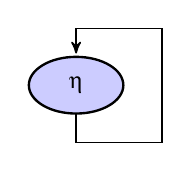
\begin{tikzpicture}[->,>=stealth',shorten >=1pt,auto,
node distance=2.5cm,
semithick,scale=0.8, transform shape,scale=0.6]

\tikzstyle{every state}=[ellipse, minimum width=2.5cm, minimum height=1.5cm, text centered, 
fill=blue!20,draw=none,text=black, draw,line width=0.3mm, font=\LARGE]

%start state
\node[state]
(init) 
{$\eta$}; 

\draw[->] (init.south) 
|- ($(init.south) + (0, -0.75cm)$) 
-| ($(init.east) + (1cm, 0)$) 
|- ($(init.east) + (0, 1.5cm)$) 
-| (init.north);

\end{tikzpicture}

	\end{subfigure}%
	\begin{subfigure}[h]{0.33\textwidth}
		\vspace{3mm}
		\begin{lstlisting}
		loop
		emit y(run_XOR_ANN_n(?x1, ?x2));
		pause;
		end
		\end{lstlisting}
	\end{subfigure}
	\caption{Mono-periodic `black-box' execution, $WCRT = \eta$}
	\label{fig:tca-bb-n}
\end{figure}

It can be noted that by Proposition~\ref{lemma1}, any \ac{ANN} implemented using the approach in Figure~\ref{fig:tca-bb-n} is also an instance of \ac{SNN} defined using Definition~\ref{def:sann}.
%\pr{This is same as the lemma in section 2. Do we need this?}

\begin{theorem}
	\label{thm:bb-soundness}
	(Soundness) A mono-periodic \ac{SNN} given an input vector $\mathbf{i}$
	produces an output vector $\mathbf{o}$ in a given tick \miff the corresponding \ac{MLP} 
	given the same input vector $\mathbf{i}$ produces the identical output vector $\mathbf{o}$ during any execution.
	
	%The synchronous execution of a ``black-box'' function $n$ will give the same output values $O$ for the same input values $I$ as the non-synchronous execution of the
	%\ac{MLP} $n$.
\end{theorem}

\begin{proof}
	The proof of Theorem~\ref{thm:bb-soundness} trivially follows from the
	fact that synchronous execution of a black-box function does not change
	the mathematical properties of that function. %, as all Esterel function
	%calls are state-less and  side effect free.
\end{proof}

\ignore{
	
	\begin{equation}
	y = f\Big(b + \sum_{i=1}^{n} \left(x_i \times w_i\right)\Big)
	\label{eqn:artificial-neuron}
	\end{equation}
	
	In the XOR example, each neuron has a \textit{threshold step function} as its activation function $f$, and has zero bias $b$.
	Hence, each neuron in the \textit{hidden} and \textit{output} layers is following Equation~\ref{eqn:xor-neuron}.
	
	\begin{example}
		In our XOR \ac{ANN}, let $i_1 = 1$ and $i_2 = 0$. \\
		Then, as $1 \times 1 \geqslant 1$, $h_1y = 1$. \\
		However, $\big(\left(1 \times 0.5\right) + \left(0 \times 0.5\right)\big) \ngeqslant 1$, so $h_2y = 0$.
		Likewise, $h_3y = 0$.  \\
		Then, as $\big((1 \times 1) + (0 \times -2) + (1 \times 1)\big) \ngeqslant 1$, the final output $o_1y = 1$.  \\
		This is correct, as $1$ \textit{xor} $0 = 1$.
	\end{example}
}

\begin{figure}[h]
	\centering
	\begin{subfigure}[h]{0.6\textwidth}
		\centering
		\begin{subfigure}[h]{0.3\textwidth}
			\centering
			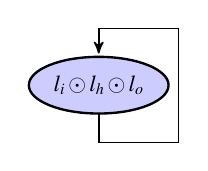
\begin{tikzpicture}[->,>=stealth',shorten >=1pt,auto,
node distance=2.5cm,
semithick,scale=0.8, transform shape,scale=0.6, font=\huge]

\tikzstyle{every state}=[ellipse, minimum width=2cm, minimum height=1.5cm, text centered, 
fill=blue!20,draw=none,text=black, draw,line width=0.3mm, font=\LARGE]

%start state
\node[state]
(init) 
{$l_i \odot l_h \odot l_o$}; 

\draw[->] (init.south) 
|- ($(init.south) + (0, -0.75cm)$) 
-| ($(init.east) + (0.25cm, 0)$) 
|- ($(init.east) + (0, 1.5cm)$) 
-| (init.north);

\end{tikzpicture}

		\end{subfigure}%
		\begin{subfigure}[h]{0.66\textwidth}
			\vspace{3mm}
			\begin{lstlisting}
			loop
			call run_XOR_ANN_li()(?x1, ?x2);
			call run_XOR_ANN_lh();
			emit y(run_XOR_ANN_lo());
			pause;
			end
			\end{lstlisting}
		\end{subfigure}
	\end{subfigure}
\caption{Mono-periodic `layer by layer' execution, $WCRT = l_i \odot l_h \odot l_o$}
\label{fig:tca-bb}
\end{figure}

\begin{figure}[h]	
	\centering
	\vspace{5mm}
	\begin{subfigure}[h]{0.5\textwidth}
		\centering
		\begin{subfigure}[h]{0.3\textwidth}
			\centering
			\begin{tikzpicture}[->,>=stealth',shorten >=1pt,auto,
node distance=2.5cm,
semithick,scale=0.8, transform shape,scale=0.6, font=\huge]

\tikzstyle{every state}=[ellipse, minimum width=2.5cm, minimum height=1.5cm, text centered, 
fill=blue!20,draw=none,text=black, draw,line width=0.3mm, font=\LARGE]

%start state
\node[state]
(l0) 
{$l_i$};

\node[state]
(l1) [below of=l0]
{$l_h$}; 

\node[state]
(l2) [below of=l1]
{$l_o$};  

\path[->] (l0) edge (l1);
\path[->] (l1) edge (l2);

\draw[->] (l2.south) 
|- ($(l2.south) + (0, -0.75cm)$) 
-| ($(l2.east) + (1cm, 0)$) 
|- ($(init.east) + (0, 1.5cm)$) 
-| (init.north);

\end{tikzpicture}

		\end{subfigure}%
		\begin{subfigure}[h]{0.66\textwidth}
			\begin{lstlisting}
			loop
			call run_XOR_ANN_li()(?x1, ?x2);
			pause;
			call run_XOR_ANN_lh();
			pause;
			emit y(run_XOR_ANN_lo());
			pause;
			end
			\end{lstlisting}
		\end{subfigure}
	\end{subfigure}
\caption{Multi-periodic `layer by layer' execution, $WCRT = l_i \oplus l_h \oplus l_o$}
\label{fig:tca-layers}
\end{figure}

\begin{figure}[h]
	\centering
	\vspace{5mm}
	\begin{subfigure}[h]{0.8\textwidth}
		\centering
		\begin{subfigure}[h]{0.3\textwidth}
			\centering
			\begin{tikzpicture}[->,>=stealth',shorten >=1pt,auto,
node distance=2.5cm,
semithick,scale=0.8, transform shape,scale=0.6, font=\huge]

\tikzstyle{every state}=[ellipse, minimum width=2.5cm, minimum height=1.5cm, text centered, 
fill=blue!20,draw=none,text=black, draw,line width=0.3mm, font=\LARGE]

%start state
\node[state]
(l0) 
{$i_1 \odot i_2$};

\node[state]
(l1) [below of=l0]
{$h_1 \odot h_2 \odot h_3$}; 

\node[state]
(l2) [below of=l1]
{$o_1$};  

\path[->] (l0) edge (l1);
\path[->] (l1) edge (l2);

\draw[->] (l2.south) 
|- ($(l2.south) + (0, -0.75cm)$) 
-| ($(l2.east) + (1.5cm, 0)$) 
|- ($(init.east) + (0, 1.5cm)$) 
-| (init.north);

\end{tikzpicture}

		\end{subfigure}%
		\begin{subfigure}[h]{0.66\textwidth}
			\begin{lstlisting}
			loop
			[
			call run_XOR_ANN_i1()(?x1);
			|| 
			call run_XOR_ANN_i2()(?x2);
			];
			pause;
			[
			call run_XOR_ANN_h1()();
			||
			call run_XOR_ANN_h2()();
			||
			call run_XOR_ANN_h3()();
			];
			pause;
			emit y(run_XOR_ANN_o1());
			pause;
			end
			\end{lstlisting}
		\end{subfigure}
	\end{subfigure}
\caption{Multi-periodic, neuron-by-neuron execution, $WCRT = \left(i_1 \odot i_2\right) \oplus \left(h_1 \odot h_2 \odot h_3\right) \oplus o_1$}
\label{fig:tcas-xor}
\end{figure}

As mentioned, using the approach in Figure~\ref{fig:tca-bb-n} to implement complex \acp{ANN} i.e. \acp{CNN} may lead to implementations that violate their timing requirements. 
The synchronous approach, however, enables efficient implementations via compositional modelling.
Esterel supports this via statements such as \texttt{pause} that help to create smaller ticks, \texttt{;} for indicating sequence operation, and \texttt{||}, which enables the modelling of concurrency. 

For example, the \ac{MLP} in Figure~\ref{fig:tca-bb-n} can also be
compositionally modelled by splitting the neural function $\eta$
into its constituent layers $l_i$, $l_h$, and $l_o$. 
While this maintains the overall functionality of the network, it
reduces the \ac{WCRT} by making the network multi-periodic, where each
period is shorter. 
As previously mentioned, the \ac{ESS} case study in Section~\ref{sec:results} examines the benefits of this approach.

%This has no major effect in Figure~\ref{fig:tca-bb}, where the network is still running in a single tick, as function $f$ will call these layers internally anyway.
%However, if \texttt{pause} statements are introduced between each layer, then the timing of the program changes significantly: 
%the \ac{WCRT} of the program will decrease, and the execution becomes `multi-cyclic'.
%Now, multiple \textit{ticks} are required to complete the execution of the neural network, but the program's responsiveness can be increased.

\begin{prop}
	%As long as a neural network's layers are still executed in
	%the correct order, the output will be correct after the last
	%layer is completed.
	The mono-periodic implementation of the XOR \ac{MLP} is functionally
	equivalent to the multi-periodic implementation.
\end{prop}

\begin{proof}
	For any input, output vectors $\mathbf{i, o}$ respectively, 
	$\eta\left(\mathbf{i}\right) = l_o\left(
	l_h\left( l_i\left( \mathbf{i} \right) \right) \right) =
	\mathbf{o}$
	%The proof of this follows intuitively as the operation of $\nu$ already recursively calls each layer $l \in L$ of neurons during execution --- we just remove one layer of indirection.
\end{proof}

\ignore{
	\begin{example}
		In the XOR \ac{MLP}, there are three layers $L = \{l_i, l_h, l_o\}$. 
		During execution, $\eta$ will invoke each layer in order as it executes each neuron. 
		We can make this explicit by calling layers as functions. 
		In this case, $\eta\left(i\right) = l_o\left(
		l_h\left( l_i\left( i \right) \right) \right) = o$
	\end{example} %\pr{While I agree that this result should hold, it is
	%unclear how function composition is actually happening in the
	%code. Code only provides a sequence of function calls without
	%showing the composition!}
}

\ignore{
	For example, a \ac{MLP} $n$ may be compositionally modelled using its constituent layers $l_i$, $l_h$, and $l_o$, as shown in Figure~\ref{fig:tca-bb} (b), (c) and (d).
	\pr{Explain each approach and the trade off. What is the distinction between approach (a) and (b)? Also, could we have just one theorem to 
		state that all approaches are equivalent i.e. they produce the same output albeit in different ticks.}
	
	\begin{lemma}
		A single-tick `layer by layer' execution of functions $l \in L$ the same output as executing function $n$ if all layers are executed in order.
	\end{lemma} 
}




\ignore{
	This has not reduced the \ac{WCRT} of the system, as $n$ has the same \ac{WCRT} as the sum of the three layers that make it up.
	However, if the layers are split over \emph{multiple ticks}, then the system \ac{WCRT} can reduce.
	
	An example of this multi-tick `layer by layer' approach is presented in Figure~\ref{fig:tca-layers}.
	
	\begin{lemma}
		A multi-tick `layer by layer' execution of layers $l \in L \in n$ will give the same output as executing network $n$ completely, iff all layers are executed in order and once a number of ticks equivalent to the number of layers has elapsed. I.e. the number of logical ticks $= |L|$.
	\end{lemma}
	The proof of this is \todo{?}
}

Observe that the response time of the multi-periodic implementation is
$3 \times T_2$, where $T_2$ is the \ac{WCRT} of the multi-periodic
version. In contrast, the response time as well as the reaction time
of the mono-periodic version is always its \ac{WCRT} $T_1$. However, it is
expected that $T_2 << T_1$.
%It is important to note that a multi-tick execution of an \ac{SNN} will not speed up the generation of outputs of the overall network --- as now, multiple ticks must be completed before a given output will be ready. 
%However, the length of each individual tick is reduced, which means that overall the system interactivity can be increased.

Like the breaking up of the function $\eta$ into its component
layers, we can also break each layer $l$ into its component neurons.
This option is presented in Figure~\ref{fig:tcas-xor}. 
Unlike in Figure~\ref{fig:tca-bb}, neurons are able to operate concurrently within each layer. 
This could provide benefits when considering multi-core
implementations such as in \cite{yuan2011compiling}.
\ignore{ however, for single-core single-threaded execution (the focus of this paper), this approach does not considerably alter tick length.} 

A summary of these approaches is presented in Table~\ref{tbl:sann-approaches}.
%we separated each neuron call with \texttt{pause} statements --- i.e. called each neuron in its own tick. 
\begin{table}[h]
	\centering
	\caption{Summary of \ac{SNN} approaches and their relevant figures, \ac{WCRT}, cycles and response time}
	\label{tbl:sann-approaches}
	\begin{tabular}{|l|l|l|l|l|}
		\hline
		Arrangement    & Figures & WCRT & Cycles & Response Time   \\ \hline
		Mono-periodic  & \ref{fig:tca-bb-n},\ref{fig:tca-bb} & High & 1 & == WCRT              \\
		Multi-periodic & \ref{fig:tca-layers},\ref{fig:tcas-xor}& Low  & \textgreater{}1 & \textgreater{}\textgreater{}WCRT \\ \hline
	\end{tabular}
\end{table}


\ignore{ 
	\pr{I suggest we use consistent terminology i.e. mono-cyclic TCA and multi-cyclic TCA and their corresponding Esterel implementation. Ideally, the proof of the theorem 
		can be done using induction. Consider a mono-cyclic implementation and multi-cyclic implementation of length $k$.
		Base case -- first time outputs after 1 tick and k ticks are same. Hypothesis -- outputs after $m$ executions are equivalent i.e. First network executed for 
		$m$ ticks while the second network executed for $k\ times m$ ticks and produced the same output starting from the same input. Proof: to show that this holds for $m+1$ executions.}
}

%\subsection{Implementing `Black-Box' \ac{SNN} in Esterel}

%The basic programming unit in Esterel is a \textit{module}. 
%Each module contains an interface declaration, followed by a body of executable statements.
%Variables are known as \textit{signals}, and may consist of a \textit{status} and a \textit{value} component. 
%Signals with only a status signals are denoted \textit{pure}, while those that contain values are instead denoted \textit{valued}.
%Sections of code may be separated with either the `\code{;}' or `\code{||}' operator, which denote sequencing and synchronous concurrency respectively.
%In order to perform manipulation of valued signals, Esterel can call external functions (provided in supplementary C files).

%Presented in Listing~\ref{lst:blackbox} and Listing~\ref{lst:blackbox-composition} are the simplest way of implementing neural networks in Esterel, already seen in the AI-BRO example.
%As can be seen, entire \acp{ANN} can be composed together and are simply called as external function calls, and will run each tick. 
%Networks can be composed together
%This can be considered the `bare minimum' to qualify as a \ac{SNN}, as the network is now running synchronously with its environment.

%Even though this implementation is quite trivial, it can still gives a strong advantage over a general-purpose implementation: when considering the methodology for composing multiple \acp{ANN}. 
%For example, consider a system that needs three \acp{ANN}, each performing a different task (as is the case in our AI-BRO example, in Section~\ref{sec:motivating-example}). 

%We can compose these multiple \acp{ANN} synchronously in Esterel. 
%As an example of this, consider an extension of our XOR network that computes $y = \big((x_1$ \textit{xor} $x_2)$ \textit{xor} $(x_3$ \textit{xor} $x_4)\big)$ (i.e. $y$ is $true$ when an odd number of inputs are $true$).
%We can compose this together still using the `black-box' methodology, as presented in Listing~\ref{lst:blackbox-composition}.
%Here, it can be seen that the first two \acp{ANN} can be run concurrently with one another, and the third \ac{ANN} can only be run when the first two are complete.



\section{Defining Runtime Enforced Synchronous Neural Networks}
\label{sec:definitions}

\subsection{\ac{VDTA}: Defining Safety Policies for \ac{CPS}}

\ignore{
We consider our industrial \ac{CPS} systems to have finite ordered sets of input values ${I} = \{{i_1}, {i_2}, \ldots {i_n}\}$ and output values ${O} = \{{o_1}, {o_2}, \ldots {o_n}\}$, where input and output values ${i_n}$ and ${o_n}$ are typed finite binary values.
However, for the purpose of the \ac{AV} case study used in this chapter, the input and output values ${i_n}$ and ${o_n}$ are fixed-point values, taking the form of 32-bit signed integer values.
The input alphabet is ${\Sigma_I} = 32^{{I}}$, i.e. the set made of all possible input value sets; and the output alphabet ${\Sigma_O} = 32^{{O}}$ is likewise the set made of all possible output value sets.
Finally, the input-output alphabet ${\Sigma} = {\Sigma_I} \times {\Sigma_O}$. 
Each input and output event is denoted as a complete set of values, and an input-output event or reaction is of the form $({x_i}, {y_i})$, where ${x_i} \in {\Sigma_I}$ and ${y_i} \in {\Sigma_O}$. 

\begin{example}
	\label{ex:io}
	Within our \ac{AV} braking example, using the \ac{VDTA} defined by the $\mathcal{V}_{ped}$ safety policy represented by Figure~\ref{fig:avpedrte}, let ${I} = \{{O_2}, {O_5}, {O_{2_v}}, {O_{5_v}}, {S}\}$ which are 32-bit signed integers representing objects 2 and 5 in the system, their velocities and the speed of the vehicle respectively.
	Then, let the output ${O} = \{{D}\} = \{{\langle A, B_S, B_H \rangle}\}$, where ${D}$ is a vector of signed 32-bit integers, representing the \textit{decision} (action) taken by the vehicle this tick (\textit{Accelerate}, \textit{Soft Brake} and \textit{Hard Brake}).
	
	Then the input-output event ${O_2}=65536$, ${O_5}=0$, ${O_{2_v}} = 655360$, ${O_{5_v}} = 0$,  ${S} = 4063232$, ${D} = \langle 0, 0, 65536 \rangle$ is denoted as:\\$(\{65536, 0, 655360, 0, 4063232\}, \{\langle 0, 0, 65536 \rangle\})$ where each value is a fixed-point (32-bit signed integer) representation of a floating point value, i.e. Object 2 is a pedestrian, Object 5 is nothing, Object 2 is travelling at 10 km/h, Object 5 is not moving, and the vehicle's speed is 62 km/h, while the decided action for this tick is hard braking ($B_H$).
\end{example}
}



We consider our industrial \ac{CPS} systems to have finite ordered sets of valued input channels ${I} = \{{i_1}, {i_2}, \ldots {i_n}\}$ and valued output channels ${O} = \{{o_1}, {o_2}, \ldots {o_n}\}$.



A VDTA can be seen as a DTA with finite set of locations, and a finite set of discrete clocks used to represent time evolution, extended with internal variables and external input (resp. output channels) called as external variables used for representing system data.
In a VDTA, a transition consists of an action carrying values of external variables, a guard on internal variables, external variables and clocks, and an assignment of internal variables, and reset of clocks.
In a VDTA, internal variables are used for internal computation, and
external variables model the data carried by the actions from the monitored system (resp. environment). 
%Thus, each input (resp. output channel) is considered as an external variable. 

%
For a variable (resp. channel) $v$, ${\cal D}_v$ denotes its domain,
and for a tuple of variables $V= (v_1, \ldots, v_n)$,
${\cal D}_V$ is the product domain ${\cal D}_{v_1} \times \cdots \times {\cal D}_{v_n}$.
%A predicate $P(V)$ on a tuple of variables $V$ is a logical formula whose semantics is a function ${\cal D}_V \rightarrow \{\true, \false\}$.
A valuation of the variables in $V$
is a mapping $\nu$ which maps every variable $v \in V$ to a value $\nu(v)$ in ${\cal D}_v$.
%
Let $X=\{x_1,\ldots, x_k\}$ be a finite set of integer variables (i.e., discrete clocks).
%
A {\em valuation} for $x$ is an element of $\bbn$, that is a function from $x$ to $\bbn$.
The set of valuations for the set of clocks $X$ is denoted by $\chi$.
%
For $\chi\in\bbn^V$, $\chi+1$ is the valuation assigning $\chi(x)+1$ to each clock variable $x$ of $X$.
Given a set of clock variables $X' \subseteq X$, $\chi[X' \leftarrow 0]$ is the valuation of clock variables $\chi$ where all the clock variables in $X'$ are assigned to $0$.

Monitors input and output words. A word is a sequence $\sigma = e_1\cdot e_2 \cdots e_n$ where $\forall i \in [1,n]: e_i = a_i(\eta_i)$ where $a_i \in \Sigma$ is an action and $\eta_i \in {\cal D}_V$ is a vector of values of a tuple of variables $V$. 


%
\begin{definition}[Syntax of {VDTA}s]
	\label{def:vdta}
	A {VDTA} is a tuple \\
	$\calA = \left(\Sigma, L, {l_0}, X, V, C, \Theta, F,  \Delta \right)$ where:
	\squishlist
	\item $\Sigma$ is a non-empty finite set of actions,
	and an action $a \in \Sigma$ has a signature $sig(a) = ( t_0, t_1, \ldots, t_k )$ which is a tuple of types of the external variables,
	\item $L$ is a finite non-empty set of locations, with $l_0 \in L$ the initial location, and $F \subseteq L$ the set of accepting locations;
	\item $X$ is a finite set of discrete clocks;
	\item $V$ is a tuple of typed internal variables \item $C$ is a tuple of external variables, where $C = I \cup O$, where $I$ is the set of input channels, and $O$ is the set of output channels; 
	\item $\Theta\subseteq {\cal D}_{V }$ the initial condition, is a computable predicate over $V$;
	\item $\Delta$ is a finite set of transitions, and each transition $t \in \Delta$ is a tuple $( l, a, c, G, A, l' )$
	also written\\
	$l \xrightarrow{a(c), G(V,c), V':=A(V,c)} l'$
	such that,
	\squishlist
	\item[\textbullet] $l, l' \in L$ are respectively the origin and target locations of the transition;
	\item[\textbullet] $a \in \Sigma$ is the action, and $c=( c_1, \ldots c_k )$ is a tuple of external variables local to the transition;
	\item[\textbullet] $G = G^D \wedge G^X$ is the guard where
	\squishlist
	\item[-] $G^D \subseteq {\cal D}_V \times {\cal D}_{sig(a)}$
	is a computable predicate over internal variables and external variables  in $V \cup c$;
	\item[-] $G^X$ is a clock constraint over $X$ defined as a Boolean combinations of constraints of the form $x \sharp f(V \cup c)$, where $x \in X$ and $f(V \cup c)$ is a computable function, and $\sharp \in \{ <, \leq, =, \geq, > \}$;
	\squishend
	\item[\textbullet] $A$$=$$(A^D, A^X)$ is the assignment of the transition where
	\squishlist
	\item[-] $A^D :{\cal D}_V \times {\cal D}_{sig(a)} \rightarrow {\cal D}_V$ defines the evolution of internal variables.
	\item[-] $A^X \subseteq X$ is the set of clocks to be reset.
	\squishend
	\squishend
	\squishend
\end{definition}
%

\begin{example}
	The case study can be presented by four, different \acp{VDTA}; $\mathcal{V}_{ped}$, $\mathcal{V}_{car}$, $\mathcal{V}_{drive}$ and $\mathcal{V}_{cnn}$, as depicted in Figures~\ref{fig:avpedrte}, \ref{fig:avcarrte}, \ref{fig:avdriverte} and \ref{fig:avcnnrte} respectively. 
	For the purposes of these examples, the \ac{VDTA} for the pedestrian safety policy, $\mathcal{V}_{ped}$, is used.
	This \ac{VDTA} specifies that driving into a pedestrian in-front (if any) and not braking hard is a violation, and approaching a pedestrian from a distance (if any) and not starting to slow down (braking softly) is a violation.
	
	This is encoded as a \ac{VDTA} with a set of locations $L = \{l_{drive}, l_{brake}, l_v\}$ and accepting locations $F = \{l_{drive}\}$, with the initial state being $l_{drive}$.
	The set of external variables $C = \{O_2, O_5, O_{2_v}, O_{5_v}, S, A, B_S, B_H\}$ are all 32-bit signed integers, where $O_2$, $O_5$, $O_{2_v}$, $O_{5_v}$ and $S$ are input channels and $A$, $B_S$ and $B_H$ are output channels.
	The set of actions $\Sigma = \{tk(O_2, O_5, O_{2_v}, O_{5_v}, S, A, B_S, B_H)\}$, and the set of internal variables $V = \{T_{lim}\}$, where $T_{lim}$ is a 32-bit signed integer.
	In the example, $\tau$ is a function with $O_2$, $O_5$, $O_{2_v}$, $O_{5_v}$ and $S$ as input parameters. 
	
	In this \ac{VDTA} there are two violation transitions, labelled \textcircled{a} and \textcircled{b} in Figure~\ref{fig:avpedrte}.
	\textcircled{a} occurs when the vehicle does anything else other than braking when there is a pedestrian in-front or not braking when there is no pedestrian ahead of the vehicle.
	\textcircled{b} can also occur when the vehicle has not braked enough within a certain period of time $T_{lim}$, or when the vehicle remains braking longer than is safe or necessary.
	This represents the vehicle taking further unsafe actions when already in an unsafe state.
\end{example}

Policy \ac{VDTA} are required to be \textit{deterministic}, i.e. for any given state, the conjunction of any guards of any other outgoing transitions may not be satisfiable; and \textit{complete}, i.e. for any given state at any given time and any given event, at least one transition guard is satisfied.

\subsection{Semantics for \ac{VDTA}}

Let $\calA = \left(\Sigma, L, {l_0}, X, V, C, \Theta, F,  \Delta \right)$  be a VDTA.
The semantics of $\calA$ is a timed transition system,
where a state consists of a location, and valuations of internal variables $V$ and clocks $X$, and actions associated with values of external variables in $C$.

\begin{definition}[Semantics of {VDTA}s]
	\label{def:vdta:semantics}
	The semantics of $\calA$ is a timed transition system $\sem{\calA}=( Q, q_0, Q_F, \Gamma, \to )$, defined as follows:
	\squishlist
	\item $Q = L \times {\cal D}_V \times \bbn^V$, is the set of states of the form $q= ( l,\nu ,\chi )$ where
	$l \in L$ is a location,
	$\nu \in {\cal D}_V$ is a valuation of internal variables,
	$\chi$ is a valuation of clocks;
	\item $Q_0 = \{ ( l_0,\nu, \chi_{[X \leftarrow 0]} )  \mid \Theta(\nu)=\true \}$ is the set of initial states;
	\item $Q_F = F \times {\cal D}_V \times \bbn^V$ is the set of accepting states;
	\item $\Gamma = \{ a(\eta) \mid
	a \in \Sigma \wedge \eta \in {\cal D}_{sig(a)}  \}$ is the set of transition labels;
	\item $\to\subseteq Q\times \Gamma\times Q$  the transition relation
	is the smallest set of transitions of the form
	$( l,\nu,\chi \rangle \longrightarrow {a(\eta)} \langle l',\nu',\chi')$
	such that  $\exists ( l, a, c, G, A, l' ) \in \Delta$,
	with $G^X(\chi + 1) \wedge G^D(\nu, \eta) $ evaluating to {\true},
	$\nu'= A^D(\nu, \eta)$ and $\chi'=(\chi+1)[A^X \leftarrow 0]$.
	\squishend
\end{definition}


%The set of timed words over $\Sigma$ where the actions carry parameter value and other data is denoted by $\tw(\Lambda)$.
A {\em run} $\rho$ of $\sem{\calA}$ from a state $q\in Q$ over a {\em trace} $w =  a_1(\eta_1)\cdot a_2(\eta_2)\cdots a_n(\eta_n)$ is a sequence of moves in $\sem{\calA}$:
$\rho = q \xrightarrow {a_1(\eta_1)} q_1
\cdots q_{n-1}\xrightarrow {a_n(\eta_n)} q_{n}$,
for some $n\in\bbn$.
The set of runs from the initial state $q_0\in Q$,  is denoted $\Run(\calA)$ and $\Run_{Q_F}(\calA)$ denotes the subset of those runs {\em accepted} by $\calA$, i.e.,  ending in an accepting state $q_n \in Q_F$.

%%%%%%%%%%%%%%%%%%%%%%%%%%%%%%%%%%%%%%%%%%%%%%%
%%%%%%%%%%%%%%%%%%%%%%%%%%%%%%%%%%%%%%%%%%%%%%%
\ignore{
\begin{example}[Run of a VDTA]
	Let us consider the VDTA discussed in Example\ref{eg:vdta} presented in Figure\ref{fig:vsa-overcurrent}. 
	An example run of the VDTA presented in Figure~\ref{fig:vsa-overcurrent} is presented here.
	Let the internal variable $i_{max}$ be initialized with 10000.
	A run of this VDTA starting from the initial state $(l_{safe}, i_{max}=10000, x = 0)$ for the word $\sigma = tk(4000, 5000,1)\cdot tk(8000, 5000,1)\cdot tk(7000, 5000,1)\cdot tk(8000, 5000,1)\cdot tk(8000, 5000,1)\cdot tk(8000, 5000,1)$ is given below:\\
	
	$(l_{safe}, i_{max}=10000, x = 0)\xrightarrow {tk(4000, 5000,1)} (l_{safe}, i_{max}=10000, x = 1)
	\xrightarrow {tk(8000, 5000,1)}
	(l_{unsafe}, i_{max}=10000, x = 0)
	\xrightarrow { tk(7000, 5000,1)}
	(l_{unsafe}, i_{max}=10000, x = 1)
	\xrightarrow { tk(8000, 5000,1)}
	(l_{unsafe}, i_{max}=10000, x = 2)
	\xrightarrow { tk(8000, 5000,1)}
	(l_{unsafe}, i_{max}=10000, x = 3)
	\xrightarrow { tk(8000, 5000,1)}
	(l_{vio}, i_{max}=10000, x = 4)
	$
\end{example}
}


\begin{example}[Run of a VDTA]
	\label{ex:run}
	An example run of the VDTA presented in Figure~\ref{fig:avpedrte} is presented here.
	Assume that the time the vehicle has to be braking is $T_{lim} = 2$. 
	The starting state is $l_{drive}$, and the first I/O event is $(\{0, 0, 0, 0, 4063232\}, \{\langle 0, 0, 0 \rangle\})$, i.e. nothing is detected in-front of the vehicle and the vehicle does not accelerate or brake, meaning it is cruising at 62 km/h.
	Thus, the automaton remains in state $l_{drive}$.
	Next tick, $(\{0, 65536, 0, 655360, 4063232\}, \{\langle 0, 65536, 0 \rangle\})$ occurs, i.e. a pedestrian is detected quite far ahead of the vehicle, moving across the road at 10 km/h, and the vehicle is taking a soft braking action from 62 km/h.
	Since ${O} = \{\langle 0, 65536, 0 \rangle\}$ which is a soft brake $B_S$ and Object 5, far ahead of the vehicle, is a pedestrian $O_5 = 65536 = O_{5_P}$ the system enters the unsafe state $l_{brake}$ and $t = 0$ is set.
	Then,  $(\{65536, 0, 0, 0, 2621440\}, \{\langle 0, 0, 0 \rangle\})$ is received, i.e. the pedestrian has stopped moving in the road and is now close to the vehicle, however the vehicle is not braking, but rather cruising at 40 km/h.
	Since no braking is detected, the violation transition $l_v$ is taken.
	As such, this run was \textit{non-accepting}.
\end{example}

\subsection{Defining Safety Automata for an \ac{AV} system}
In order for the \ac{AV} system to operate safely, it must follow a set of policies ($\mathcal{V}$), defined in English here:

$\mathcal{V}_{cnn}$: The output of the vision \ac{CNN} ensemble networks ($O$) must match the \ac{LiDAR} values ($L$) when the confidence of the ensemble networks is low. 
If the confidence is high, and there is a mismatch, the output should be classified as \textit{unknown} ($U$).
The system should treat this output as if it were a pedestrian, i.e. with utmost caution.

$\mathcal{V}_{drive}$: The vehicle may not exceed the safe speed limit. 
An \textit{acceleration} command $A$ should be suppressed when the vehicle's speed limit of 100km/h is reached.

$\mathcal{V}_{car}$: Ensure that the car does not drive into other vehicles. If an \textit{acceleration} command $A$ is asserted when the car in front (i.e. $O_{2_C}$ or $O_{5_C}$) is driving slower than the \ac{AV} ($O_{2_V}<S|O_{5_V}<S$), then this is suppressed and instead an appropriate brake speed $B_S$ (soft) or $B_H$ (hard) would be asserted instead.

$\mathcal{V}_{ped}$: Ensure that the car does not behave unsafely around pedestrians. If a pedestrian appears in-front of the vehicle $P=true$, then the car should select an appropriate braking action (either $B_S$ or $B_H$). If a pedestrian remains off to the side of the vehicle, then either the vehicle should cruise or a braking action is appropriate.

We can define these rules of the \ac{AV} system as a \textit{Safety Automata}~\cite{recps}, which are a kind of \acf{DTA}. 
Examples of this are presented in Figures \ref{fig:avpedrte} - \ref{fig:avcnnrte}, which represent the automata used in the four policies of the \ac{AV} system.
%Here, $A$ refers to the accelerate action, $B_S$ refers to a slow, or gentle, braking action, $B_H$ refers to a hard braking action.
$P$ is a flag that denotes the presence of a pedestrian in a position that will be dangerous at any point in the future, and $t$ is a timer that ensures that the \ac{AV} has braked for long enough and in time when a collision with a pedestrian has been detected, denoted by the time $T_{lim}$. 
$T_{lim}$ is a predefined length of time by which the system should have reacted to a pedestrian in a dangerous position.

Finally, a complete policy framework can be established by simply ANDing the component policies together, i.e. \\ $\mathcal{V}_{av} = \mathcal{V}_{cnn} \wedge \mathcal{V}_{drive} \wedge \mathcal{V}_{car} \wedge \mathcal{V}_{ped}$.

\begin{figure}[H]
	\centering
	\includegraphics[width=\linewidth]{avpedrte.tikz}
	\caption{Safety Automaton for Policy $\mathcal{V}_{ped}$\label{fig:avpedrte}}
\end{figure}
\begin{figure}[H]
	\centering
	\includegraphics[width=0.5\linewidth]{avcarrte.tikz}
	\caption{Safety Automaton for Policy $\mathcal{V}_{car}$\label{fig:avcarrte}}
\end{figure}
\begin{figure}[H]
	\centering
	\includegraphics[width=0.5\linewidth]{avdriverte.tikz}
	\caption{Safety Automaton for Policy $\mathcal{V}_{drive}$\label{fig:avdriverte}}
\end{figure}
\begin{figure}[H]
	\centering
	\includegraphics[width=0.5\linewidth]{avcnnrte.tikz}
	\caption{Safety Automaton for Policy $\mathcal{V}_{cnn}$\label{fig:avcnnrte}}
\end{figure}


\subsection{Enforcing Non-accepting I/O Events}
Enforcers are designed to prevent a system from generating an input/output trace that is non-accepting, such as Example~\ref{ex:run}.
\cite{recps} proposed \ac{DTA} semantics with two possible methodologies for editing non-accepting I/O events.
These are \textit{random} and \textit{minimum} edits; a random edit chooses a random, accepting event from a list of accepting I/O events and minimum edit chooses the closest accepting event to the current non-accepting event.
However, neither of these edits are not always useful for problems in real scenarios.
Take Example~\ref{ex:run}, when the transition $l_{drive} \rightarrow l_v$ is taken, Object 2 can be edited such that $l_v$ is not entered, however this will not remove the danger that initially posed this transition.
However, if the action ${O}$ was changed, e.g. the cruising action in the example that caused the non-accepting trace was changed to a hard braking action, then an accepting event would have occurred \textit{and} the pedestrian in the road would have been safe.

In general, then, the designer of any given policy should also select their preferred edit actions out of the list of possible safe edits for each violation transition, thus ensuring practical runtime enforcement.

\begin{example}[Selected Edit Actions for a VDTA]
	In Figure~\ref{fig:avpedrte}, there are many different actions in $\Sigma$ that, when taken in a specific location $L$ result in a violation transition.
	In this example, a situation where the current locations is $l_{drive}$ and the action is $\Sigma = \{tk(1, 0, 10, 0, 30, 1, 0, 0)\}$, i.e. there is a pedestrian directly in front of the vehicle moving at 10 km/h, while the vehicle is moving directly forward at 30 km/h and is accelerating.
	Thus, the violation transition \textcircled{a} occurs.
	\squishlist
	\item Transition \textcircled{a}: $A := 0$, $B_S := 0$ and $B_H := 1$
	\squishend
	The recovery for this violation transition changes the vehicle to not accelerate, but rather brake hard.
	This instead changes the transition to $l_{drive} \rightarrow l_{brake}$, which is a safe transition that slows the vehicle down before it hits the pedestrian.
\end{example}
%The first policy, $\mathcal{V}_{cnn}$, compares the \ac{LiDAR} depiction and the classified image class from the corresponding ensemble outputs, if the \ac{LiDAR} and ensemble outputs are different, and the ensemble confidence value is low, the ensemble output is changed to match the output of the corresponding \ac{LiDAR} reading.
%If the ensemble confidence is high, both the \ac{LiDAR} reading and the corresponding ensemble output are changed to signal that the object detected is \textit{Unknown} and should be treated with extra caution, as if the object were a pedestrian.
%The second policy, $\mathcal{V}_{drive}$, ensures that the vehicle maintains reasonable driving practices on the road, e.g. not staying stationary in the middle of the road and not speeding.
%If the \ac{AV} controller outputs that the \ac{AV} should \textbf{accelerate} while the \ac{AV} is at the speed limit, the \textbf{accelerate} command would be changed to a  \textbf{cruise} command.
%Likewise, if the \ac{AV} controller decides that the \ac{AV} should remain stationary in an empty road, the \textbf{brake} (or \textbf{cruise}) command would be modified to an \textbf{accelerate} command.
%The third policy, $\mathcal{V}_{car}$, checks the environment for other vehicles and ensures that the \ac{AV} does not drive into other vehicles, or cause accidents with other vehicles in any way.
%If the \ac{AV} would \textbf{accelerate} into a vehicle in front, the \textbf{accelerate} would be changed to a \textbf{cruise}, if the \ac{AV} was driving much faster than the vehicle in front and the \ac{AV} is not braking, the current action would be modified to be a \textbf{brake} action.
%The fourth, and highest priority, policy ($\mathcal{V}_{ped}$) monitors the environment for pedestrians and ensures that the car does not exhibit unsafe behaviour with regards to the pedestrians. 
%If the \ac{AV} were to \textbf{accelerate}, or \textbf{cruise}, into a pedestrian that is in front of the vehicle, or approaching the road from the sides, the \textbf{accelerate}, or \textbf{cruise}, action would be changed to a \textbf{brake} action.
%If the \ac{AV} does not brake fast enough with a pedestrian in front of the \ac{AV}, or approaching from the sides, a \textbf{hard brake} action would be initiated instead of the \ac{ANN} proposed action.
%This policy ensures that the vehicle always drives slowly and cautiously around pedestrians.


\subsection{\ac{SANN}: Defining Artificial Neural Networks for \acp{CPS}}
\begin{definition}[Layer of a \ac{SANN}]
	\label{def:layer}We define the \emph{\ac{SANN} Layers} as a tuple $\mathcal{L} = (\mathcal{I}, \mathcal{O}, \mathcal{W}, \mathcal{T}, \tau)$:
	\begin{itemize}
		\item $\mathcal{I} = \{i_0, i_1, ..., i_k \}$ are the $k$ inputs to the layer, represented by a vector of 32-bit signed integers.
		\item $\mathcal{O} = \{o_0, o_1, ..., o_k \}$ are the $k$ outputs from the layer, represented by a vector of 32-bit signed integers.
		\item $\mathcal{W} = \{w_0, w_1, ..., w_k\}$ are the $k$ weights associated with the layer, represented by a vector of 32-bit signed integers.
		\item $\mathcal{T}$ is the layer type and determines the operations applied to the weights and inputs, where $\mathcal{T}~\in~\{Dense, Convolutional, Maximum~pool, Average~pool\}$.
		\item $\tau(\mathcal{I}, \mathcal{W}, \mathcal{T}) = \mathcal{O}$ is the non-linear function that produces an output set $\mathcal{O}$ given inputs $\mathcal{I}$, weights $\mathcal{W}$ and layer type $\mathcal{T}$. 
	\end{itemize}
\end{definition}

\begin{definition}[\ac{SANN}]
	\label{def:cnn}
	A \ac{SANN} is an extension of Definition~\ref{def:bb-mlp}. 
	It should be noted that the definition of a \ac{SANN} can be used to implement and run a \acf{MLP}.
	We define a \emph{\ac{SANN}} as a tuple $\mathcal{C} = (\mathcal{I}, \mathcal{O}, \mathcal{A}, \eta)$ where
	\begin{itemize}
		\item $\mathcal{I}$ is a finite collection of 32-bit signed integer input variables with the domain \textbf{I}$ = 32^n$, where $n$ is the number of inputs.
		\item $\mathcal{O}$ is a finite collection of 32-bit signed integer output variables with the domain \textbf{O}$ = 32^m$, where $m$ is the number of outputs.
		\item $\mathcal{A}$ denotes the finite set of instantiated, connected layers in the \ac{CNN}, with any assortment of layers defined by $\mathcal{L}$ in Definition~\ref{def:layer}.
		\item $\eta$: \textbf{I} $\rightarrow$ \textbf{O} is the non-linear function, termed the network function, that provides the behaviour of a given network, i.e. when provided $\mathcal{I}$ inputs produces $\mathcal{O}$ outputs. 
	\end{itemize}
\end{definition}

\begin{example}
	\label{ex:cnn}
	An example of one of the fifteen the object detection \acp{CNN} used in the the \ac{AV} case study is presented here.
	Any of the fifteen \acp{CNN} have $28 \times 28 \times 3 = 2352$, therefore \textbf{I}$~= \langle I_0, I_1 ..., I_2351 \rangle$.
	Likewise, each CNN has seven outputs resulting in \textbf{O}$~= \langle O_0, O_1 O_2 ..., O_7 \rangle$.
	Each \ac{CNN} has a set of twelve layers: $\mathcal{A} = \langle\mathcal{L}_0, \mathcal{L}_1, ..., \mathcal{L}_{11}\rangle$ defined in Definition \ref{def:layer}.
	The arrangement of layers the following: $\mathcal{A} = \langle\mathcal{L}_{Dense}, ~\mathcal{L}_{Convolutional},\\~\mathcal{L}_{Maximum~pool}, ~\mathcal{L}_{Convolutional},~\mathcal{L}_{Convolutional}, ~\mathcal{L}_{Maximum~pool},~\mathcal{L}_{Convolutional},~\mathcal{L}_{Convolutional},\\~\mathcal{L}_{Convolutional},~\mathcal{L}_{Convolutional},~\mathcal{L}_{Average~pool},~\mathcal{L}_{Dense}\rangle$.
	The network function $\eta$ runs the \ac{SANN} such that an input image of size $28 \times 28 \times 3$ produces an output vector of size $7$.
\end{example}

\subsubsection{Running a \ac{SANN}}
A \ac{SANN} can be run two different ways depending on the synchronous tick assignment of the \ac{SANN}, see Section~\ref{sec:esterel-mapping} for more on tick analysis of \ac{SNN}. 
If the entire CNN is run each tick, the \ac{SANN} is run using the function $\eta(\mathcal{I}_k) = \mathcal{O}_k$, where $\mathcal{I}_k$ are the inputs for tick $k$ and $\mathcal{O}_k$ are the outputs for tick $k$.
If only a single layer of the \ac{SANN} is run each tick, the layer at $\mathcal{A}_k$ is run as a function, where $k$ is the position of the layer in $\mathcal{A}$ of the current tick.

\begin{example}
	\label{ex:runcnn}
	An example run of one of the fifteen the object detection \ac{SANN} used in Example \ref{ex:cnn} is presented here.
	An input image of a car, $28 \times 28$ pixels in colour is given to the \ac{SANN} network function $\eta$ as the input \textbf{I}.
	These pixels are flattened into a single layer of 2352 32-bit signed integers inputs and passed to the input layer $\mathcal{L}_0$.
	These inputs are then passed to the next layer of the \ac{SANN} $\mathcal{L}_1$, in this case a convolutional layer.
	This convolutional layer has 32 filters and thus, after the 32 sets of matrix convolution, produces 32 sets of 2352 32-bit signed integer values.
	These $32 \times 2352$ values are then passed on to the next layer $\mathcal{L}_2$; a $2 \times 2$ maximum pooling layer.
	This layer takes each set of 2352 values and trims them down to $2353 / (2 \times 2) = 588$ values.
	These 32 sets of 588 values are then passed on to the next convolutional layer $\mathcal{L}_3$ with 16 filters.
	And so on.
	Until the values reach the output layer $\mathcal{L}_11$, a dense layer, where they are condensed into 7 distinct output values, making up the output matrix \textbf{O} which classifies the image with the values $\langle 0.02, 0.91, 0.03, 0.04, 0.00, 0.00, 0.00 \rangle$.
	This means that the \ac{SANN} is 91 \% confident that the input image is a vehicle, and only 2 \% confident that it is a person.
	Therefore $\eta(2352_{car}) = \langle 0.02, 0.91, 0.03, 0.04, 0.00, 0.00, 0.00 \rangle$
\end{example}

\subsection{\ac{SNN}: Defining \acp{SNN} for \acp{CPS}}
A \acf{SNN} is generally composed of, but not limited to \acp{ANN}.
A \ac{SNN} may include modules of any type, given that they are (1) synchronous and (2) fit the following definition (Definition~\ref{def:comp}):
\begin{definition}[Defining Synchronous Neural Network Components]
	\label{def:comp}
	We define a \ac{SNN} Component, 'meta component', as a tuple $\mathcal{K} = (\mathcal{I}, \mathcal{O}, \Sigma)$ where
	\begin{itemize}
		\item $\mathcal{I} = \{i_0, i_1, ..., i_k \}$ are the $k$ inputs to the meta component, represented by a vector of 32-bit signed integers.
		\item $\mathcal{O} = \{o_0, o_1, ..., o_k \}$ are the $k$ outputs from the meta component, represented by a vector of 32-bit signed integers.
		\item $\Sigma: \mathcal{I} \rightarrow \mathcal{O}$ is the non-linear function that produces outputs $\mathcal{O}$ given inputs $\mathcal{I}$. 
	\end{itemize}
\end{definition}

\begin{definition}[Defining \acp{SNN}]
	\label{def:snn}
	We define a \ac{SNN}, as an extension of the previously defined \ac{MNN} from Definition~\ref{def:nsanns}. 
	We define a \emph{\ac{SNN}} as a tuple $\mathcal{S} = (\mathcal{I}, \mathcal{O}, \mathcal{M}, \mathcal{L}, \mathcal{A}, \Delta)$ where
	\begin{itemize}
		\item We term the first meta-layer as the input meta-layer and the last one as the output meta-layer.
		\item  $\mathcal{I}=I_1 \cup .. \cup I_k$, where $I_1..I_k$ are the inputs of the meta components in the input meta layer. If $K=|\mathcal{I}|$ then the domain is $\mathbf{I} = \mathbb{R}^K$.
		\item $\mathcal{O}=O_1 \cup .. \cup O_j$, where $O_1..O_j$ are the outputs of the meta components in the output meta layer. If $J=|\mathcal{O}|$ then the domain is $\mathbf{O} = \mathbb{R}^J$.
		\item $\mathcal{M}$ is the set $M \in \mathcal{M}$ of Synchronous \acp{CNN} $\mathcal{C}$, according to Definition~\ref{def:cnn}, and \ac{MNN} Components $\mathcal{K}$ defined in Definition~\ref{def:comp}, such any two connected meta components are IO-compatible.
		\item $\mathcal{L}$ is the set of meta-layers of various \acp{CNN} and meta components.
		\item $\mathcal{A}: \mathcal{M} \rightarrow \mathcal{L}$ is the network mapping function that maps a given \ac{CNN} or meta component to a layer.
		\item $\Delta \subset \mathcal{M} \times \mathcal{M}$ provides the mapping of IO connectivity information between \acp{CNN} and meta components of different meta-layers.
	\end{itemize}
\end{definition}

\subsubsection{Running a \ac{SNN}}
A \ac{SNN} can be run differently, depending on the tick frequency for the \ac{SNN}, similar to the running of a \ac{SANN}.
A \ac{SNN} can be run as a black box, where the inputs to the \ac{SNN} are given and, one tick later, the outputs are produced.
In this case the \ac{SNN} is run as the cumulative function of all meta components, be it \acp{SANN}, synchronous \acp{RE} or any other synchronous component, where the outputs of each component are passed to the next component, depending on the $\Delta$ function for that \ac{SNN}.

A \ac{SNN} can also be run so that each meta component is run in one logical tick, i.e. concurrent components are run at the same time and consecutive components are run in order.
Each meta component is run as a single black box function, with inputs provided at the beginning of the tick and outputs provided at the end.
At the start of each tick, each component receives its input according to the \ac{SNN} specific $\Delta$ function describing its I/O mapping.

Alternatively, a \ac{SNN} can be run tick-by-tick, such that each meta component is also run tick-by-tick.
In this case, each meta component of the \ac{SNN} can run over multiple ticks, e.g. running one layer of a \ac{SANN} every tick.

\ignore{Care has to be taken when running the \ac{SNN} like this to ensure that outputs reach the appropriate input of the next component in a synchronous manner so that deadlines are not missed and each component runs on the correct set of inputs, i.e. a \ac{SANN} component should not run until all its inputs are present.}

\begin{example}
	\label{ex:runsnn}
	An example run of the fifteen the object detection \acp{SANN}, with a single \ac{SANN}'s run described in Example \ref{ex:cnn} and the definition of each \ac{SANN} given in Definition \ref{def:cnn}, and their respective ensembles and enforcers (as shown in Figure \ref{fig:avmnn}) is presented here.
	
	The \ac{RE} used in this system has been defined in~\cite{recps}, and is enforcing the safety policy $\mathcal{V}_{cnn}$ specified by Figure \ref{fig:avcnnrte}.
	This \ac{RE} is represented as a meta component $\mathcal{K}$, where $\mathcal{I}$ is a finite vector of 32-bit signed integer \ac{SANN} inputs and $\mathcal{O}$ is a finite vector of 32-bit signed integer outputs.
	The \ac{RE} is run with the $\Sigma$ function, which applies a logical tick to the enforced \ac{VDTA} (Definition~\ref{def:vdta}) and, where necessary, \textit{edits} the meta components inputs $\mathcal{I}$ providing edited outputs $\mathcal{O}$.
	
	The ensembles shown in Figure \ref{fig:avmnn} are each defined as meta components $\mathcal{K}$, where $\mathcal{I}$ is a finite vector of 32-bit signed integer \ac{SANN} classifications and $\mathcal{O}$ is a single 32-bit signed integer classification.
	Each ensemble is run with its $\Sigma$ function, which combines its inputs $\mathcal{I}$ to produce a single, more accurate output.
	
	For the purposes of this example, the \ac{SNN} will be run such that each meta component of the \ac{SNN} is executed in one tick.
	
	Assuming the system has not been run yet, at the start of tick 1, the five input images from the five camera positions, shown in Figure \ref{fig:av}, are given to their respective \ac{SANN} ensembles.
	Each \ac{SANN} ensemble receives one image, and that image is fed to each \ac{SANN} in that ensemble such that the image is the input $\mathcal{I}$ for that \ac{SANN}.
	Over tick 1, each \ac{SANN} is run concurrently using the network function $\eta$ so that each \ac{CNN} produces one output set $\eta(\mathcal{I_{i_j}}) = \mathcal{O_{i_j}}$ at the end of tick 1, where $i$ is the ensemble number and $j$ is the number of the \ac{SANN} in that ensemble.
	At the start of tick 2, each ensemble receives its inputs $\mathcal{I}$ from each of the three connected \acp{CNN}' outputs.
	The functions $\Sigma$ of each ensemble are run concurrently over tick 2, producing an output $\mathcal{O}_i$ at the end of tick 2 for each ensemble $i$, which is the cumulative prediction of the three \ac{SANN} in that ensemble.
	At the start of tick 3, the \ac{RE} receives input from each of the five ensembles, and produces enforced outputs at the end of tick 3.
	At the start of tick 4, this process repeats.
\end{example}













%\section{\acfp{SNN}}
\label{sec:definitions}

While implementing the \ac{AV} system as a \textit{meta-network} of \acp{SANN}~\cite{sann}, statically analysing it to ensure adherence to the policy $\varphi_{av}$ would still be extremely difficult due to the usage of \acp{CNN} as the image-processing components of the system and the unknown/unpredictable nature of many of the inputs.
Instead, we propose the usage of \ac{SRE} to ensure system correctness at runtime.
We define the composition of a \ac{SANN} with \ac{SRE} as a \ac{SNN}.

\begin{definition}
	\label{def:ssann}
	An \ac{SNN} is formalised as a tuple $S = \langle I,~O,~\varphi_I,~\varphi_O,~L,~\gamma,~\alpha  \rangle$, where:
	\begin{itemize}
		\item $I$ is a finite collection of input variables with
		its domain being $\mathbf{I} = \mathbb{R}^n$.
		\item  $O$ is a finite collection of  output variables with
		its domain being $\mathbf{O} = \mathbb{R}^m$.
		\item $\varphi_I$ is an input safety policy, defined by a safety automaton~\cite{recps}, specifying the safe behaviour of inputs $I$.
		\item $\varphi_O$ is an output safety policy, defined by a safety automaton, specifying the safe behaviour of input-outputs $I \times O$.
		\item $L$ denotes a set of \ac{ANN} layers $\{l_i,~l...~,~l_{pp}\}$. Each layer is described by its layer type, starting with the input layer $l_i$ and iterating through the \ac{ANN} until the post-processing layer $l_{pp}$.
		\item $\gamma: I_l \rightarrow O_l$ is the non-linear activation function that provides the behaviour of a given layer, i.e. when provided inputs $I_l$, the layer produces outputs $O_l$.
		\item $\alpha: l_k \rightarrow l_{k+1}$ is the layer-to-layer mapping function that maps the outputs $O$ of each \ac{ANN} layer to the inputs  $I$ of the following layer. $O_k$ maps to $I_{k+1}$ such that every input of layer $k+1$ has at least one output from layer $k$ connected to it. 
	\end{itemize}
\end{definition} 

To run a given \ac{SNN} (i.e. fully complete computation over an input set $\mathbf{I}$), the functions $\gamma$ and $\alpha$ will each need to be called once for every layer (apart from the output layer, on which only $\gamma$ is called).

%\begin{figure}[t]
%	\centering
%	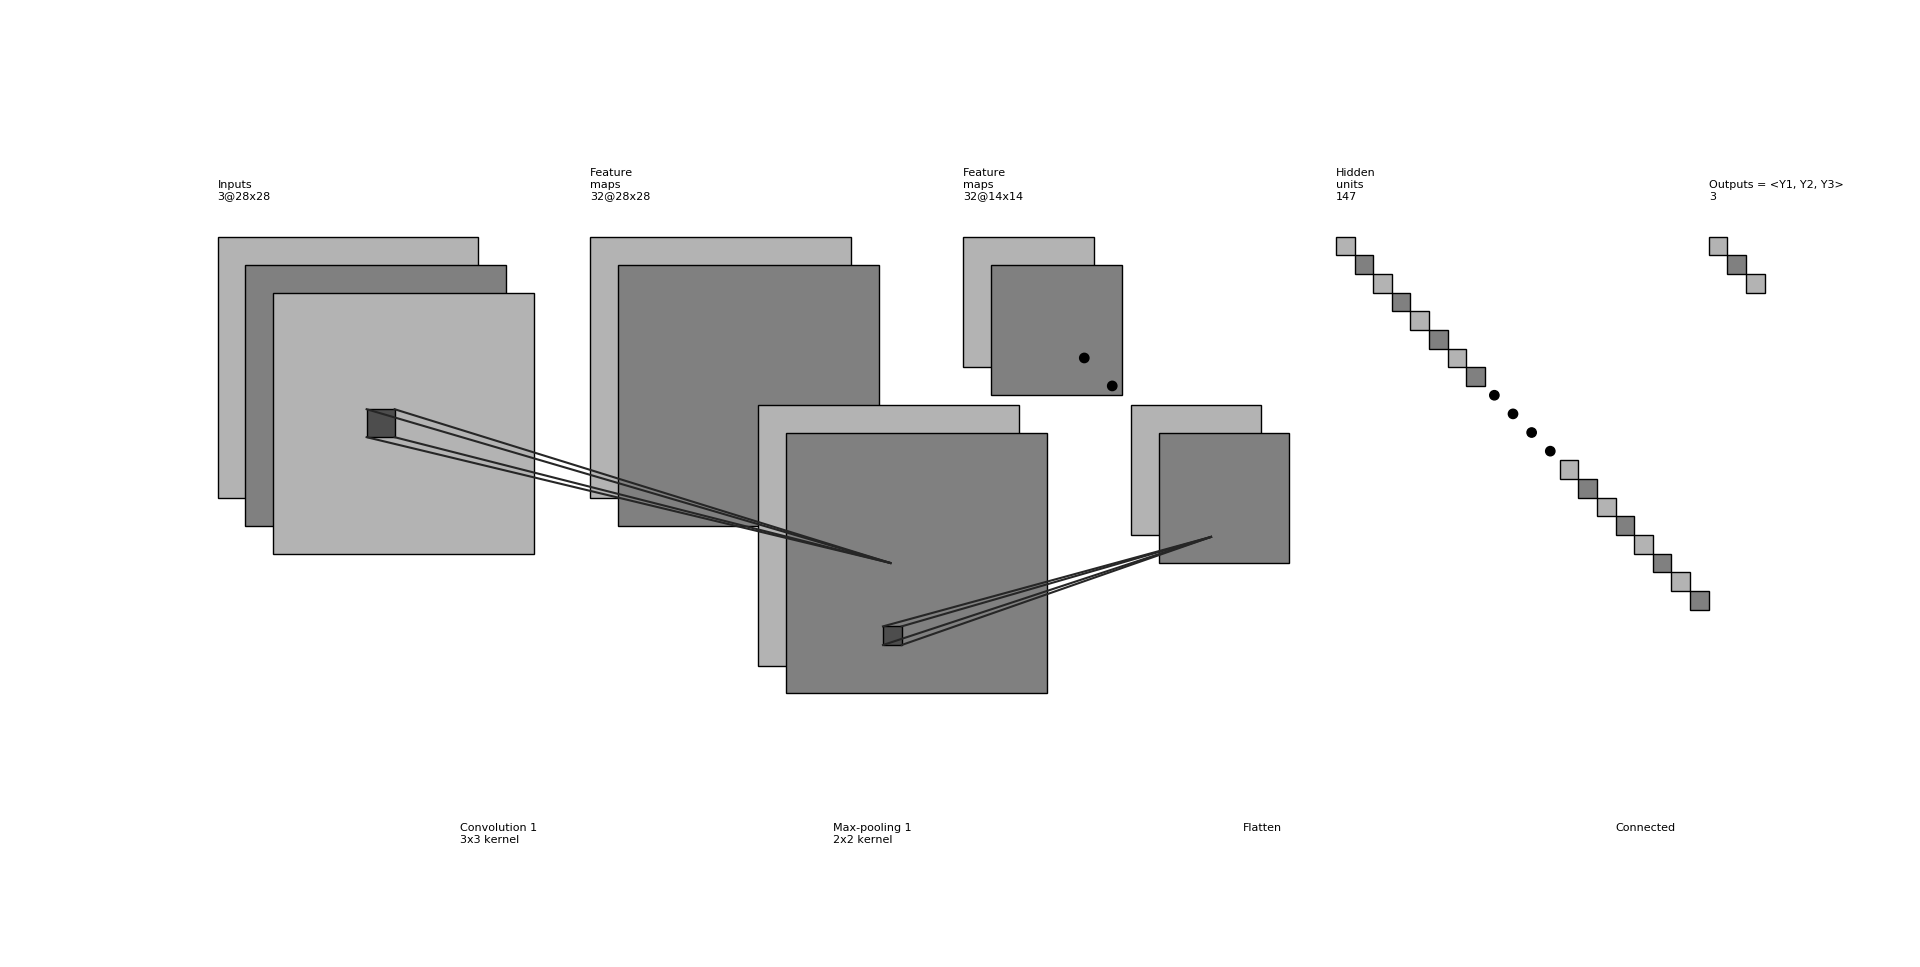
\includegraphics[width=\linewidth]{fig/CNN.png}
%	\caption{Diagram showing the structure of a basic \ac{CNN}.	\label{fig:cnn}}
%\end{figure}

\begin{figure}[b]
	\centering
	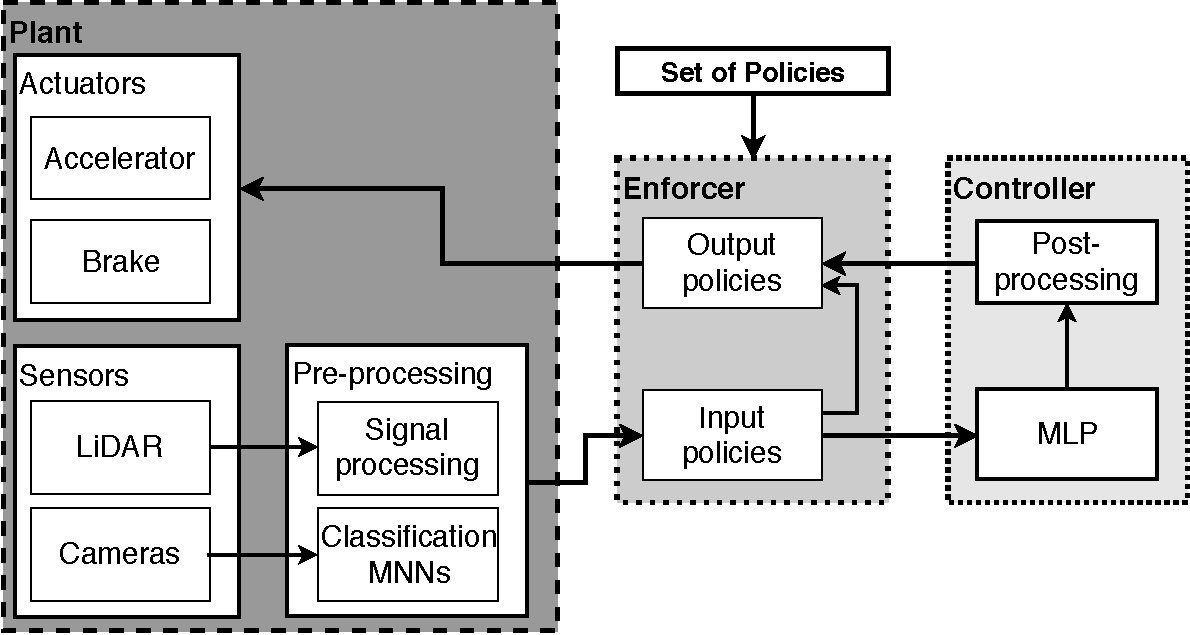
\includegraphics[width=\linewidth]{Content/fig/AV-sys.pdf}
	\caption{Diagram showing the system design for the \ac{AV}. \label{fig:avsys}}
\end{figure}

\subsection{\ac{AV} system as a \ac{SNN}}
%\todo{You have no page limit at the moment so add the other policies to this document so Partha can see them}

The \ac{AV} system described in Section~\ref{sec:case} can be demonstrated as the combination of components and connections shown in Figure~\ref{fig:avsys}.
It can be presented formally using Definition~\ref{def:ssann} with:
\begin{itemize}
	\item $I=\langle S,~P,~O_{1},~O_{1_S},~O_{1_D}...,~O_{5},~O_{5_S},~O_{5_D} \rangle$, i.e. the 17 different fixed-point integer inputs to the controller \ac{ANN} described in Section~\ref{sec:case}.
	\item $O = \langle A, B_S, B_H \rangle$ are the three different fixed-point integer outputs which represent the different actions (and the confidence in the action) that can be taken by the \ac{AV} at any given time.
	\item $\varphi_I = \varphi_{av_I} = \varphi_{cnn_I} \wedge \varphi_{ped_I} \wedge \varphi_{car_I} \wedge \varphi_{drive_I}$, i.e. the complete set of policies projected on inputs $I$. Once combined, they ensure the safety of the \ac{CNN} ensemble and \ac{LiDAR} outputs (i.e. the controller's inputs).
	\item $\varphi_O = \varphi_{av} = \varphi_{cnn} \wedge \varphi_{ped} \wedge \varphi_{car} \wedge \varphi_{drive}$, i.e. the complete set of policies ensuring the safety of the controller. Once combined, they prevent collisions with pedestrians, other vehicles and maintain that the car drives consistently and within the law.
	\item $L = \{l_i,~l_h,~l_o,~l_{pp}\}$, are the four layers of the controller \ac{ANN}, i.e. the input layer, hidden layer, and output layer of the \ac{MLP}; and the post processing layer of the controller.
	%\item The function $\gamma$ given input $\langle I_{h_1}, I_{h_2}, ..., I_{h_17} \rangle$ to the hidden layer $l_h$ produces the output vector $\langle O_{h_1}, O_{h_2}, ..., O_{h_17} \rangle$, i.e. one output for each neuron in the hidden layer. 
	%\item The function $\alpha$ maps one layer's outputs to the next layer's inputs, e.g. the inputs $I_{o}$ of the output layer $l_o$ are derived from the outputs $O_{h}$ of the hidden layer $l_h$ using $I_{o} = \langle \alpha(O_{h}) \rangle = \langle \displaystyle \sum_{j}^{i=1} O_{h_1}.w_{1_i}, \displaystyle \sum_{j}^{i=1} O_{h_2}.w_{2_i}, \displaystyle \sum_{j}^{i=1} O_{h_3}.w_{3_i} \rangle$, where $j$ is the number of neurons in the hidden layer, and $w_{m_n}$ is the hidden layer weight at corresponding to the $m^{th}$ output neuron and the $n^{th}$ hidden layer neuron. 
	%\item \todo{How does the post-processing fit into this definition? It is clearly between the MLP and the output enforcer. You may need to justify post-processing as a fourth layer of the MLP, and change the MLP to some different ANN name. I have attempted to fit this already.} 
\end{itemize}
%The network function $\eta$ given input $\langle 0, 0, ..., 0 \rangle$ produces an output $\langle 1, 0, 0 \rangle$ i.e. $\eta(\langle 0, 0, ..., 0 \rangle) = \langle 1, 0, 0 \rangle$.


The bi-directional enforcer for this system enforces the properties in Section~\ref{sec:case} %$\varphi_{av}$,
%These can be represented as \ac{DTA}, and then ANDed together to produce a single \ac{DTA}, as seen in Figure~\ref{fig:avrte}. %\todo{Figure 2 doesn't show the full DTA. This is wrong.}
%Each policy is defined by a Safety Automaton, with the pedestrian avoidance policy being a \ac{DTA}.
%The policies are combined by ANDing the states of each policy together to create a single, larger policy that includes each other policy.
%The policy is enforced using a bi-directional runtime enforcer, 
and is seen in the complete system in Figure~\ref{fig:avsys}.

\begin{example}
	Assume the system is in state $q_{drive}$ with the car cruising at 50 km/h.
	Suddenly, a pedestrian steps into the road ahead and to the left of the vehicle.
	Hence, the \ac{SNN} receives an input vector $\mathbf{I}$ describing the environment, including the vehicles current speed and the pedestrian detected on the left-most sensor.% and output a corresponding action.
	The safe reaction would be to slow down and act with caution until the pedestrian has been passed, or brake hard if the pedestrian walks in front of the vehicle.
	
	Since the ensembles correctly identified the pedestrian, and agree with the \ac{LiDAR} readings, the input enforcer $\varphi_I$ does not modify any of the inputs in $\mathbf{I}$.
	The functions $\gamma$ and $\alpha$ are called on every \ac{ANN} layer except the output layer, where only $\gamma$ is called.
	Suppose the controller \ac{ANN} is in the early stages of training and does not recognise a pedestrian walking to the road as a potential safety hazard, the \ac{ANN} outputs that nothing should be done in this situation (i.e. $\langle 0, 0, 0 \rangle$).
	The output enforcer $\varphi_O$ recognises that this is not the desired output, and initiates a braking sequence by changing the \ac{ANN} outputs to gently brake (i.e. $\langle 0, 1, 0 \rangle$) and sets the output vector $\mathbf{O}$ to the new \ac{ANN} outputs.
	The braking action, along with the positioning of the pedestrian, causes the enforcer to change to the state $q_{brake}$.
\end{example}

\subsection{Training the \ac{AV} \acp{ANN}}
Since the ideal outputs for the controller are unknown, due to the large number of states the system could be in at any given time, the system could not be trained using standard back-propagation with gradient descent.
Instead, a reinforcement learning algorithm was used for the training phase of the controller.
The algorithm rewarded vehicles that did well during the training, while penalising those that did not.
%Due to the hardware limitations, the system was trained for, at most, 10,000 epochs. 
%At 1, 10, 100, 1,000 and 10,000 epochs the state of the controller \ac{ANN} was saved and used for testing. 
%At each of the trained epochs, the aforementioned policies were enforced, and the resultant behaviour of each \ac{ANN} state was recorded.
%The results of this system are shown in Section~\ref{sec:results}.


%\begin{example}
%	The \ac{AV} system controller \ac{SNN} described in Section~\ref{sec:case} can be presented formally with:
%	\begin{itemize}
%		\item $I=\langle x_1, x_2, ..., x_{2352} \rangle$, i.e. the flattened input of the $28 \times 28 \times 3$ input image. 
%		\item $O = \langle Y_1, Y_2, Y_3 \rangle$.
%		\item $\varphi_I = \varphi_{cnn}$, i.e. the policy that modifies the \ac{CNN} ensemble outputs in the case of clashing class confidence values.
%		\item $\varphi_O = \varphi_{ped} \wedge \varphi_{car} \wedge \varphi_{drive}$, i.e. the policies that prevent collisions with pedestrians, other vehicles and maintain that the car drives consistently and within the law.
%		\item $L = \{Input, Convolution 1, ..., Connected, Output\}$, as described in Figure~\ref{fig:cnn}.
%		\item The function $\gamma$ given input $\langle I_{Maxpooling 1} \rangle$ to layer $Maxpooling 1$ produces the output vector $\langle maxpool(I_{Maxpooling 1}) \rangle$. 
%		\item The function $\alpha$ maps layer outputs to layer inputs, e.g. the inputs $I_{Maxpooling 1}$ of $Maxpooling 1$ are derived from the outputs $O_{Convolution 1}$ of $Convolution 1$ using $I_{Maxpooling 1} = \langle \alpha(O_{Convolution 1}) \rangle = \langle O_{Convolution 1} \rangle$. 
%		\item The network function $\eta$ given input image $\langle \mathbf{I_{image}} \rangle$ produces an output $\langle \mathbf{O} \rangle = \eta(\langle \mathbf{I_{image}} \rangle) = \langle P_1, P_2, ..., P_n \rangle$ where $P_1$ is the probability of the input image being the $1^{st}$ class and $P_n$ is the probability of the input image being the $n^{th}$ class.
%	\end{itemize}
%\end{example}


%\begin{figure}[t]
%	\centering
%	\scalebox{0.9}{\def\layersep{2.25cm}
\begin{tikzpicture}[shorten >=1pt,->,draw=black!100, node distance=\layersep]
	\tikzstyle{every pin edge}=[<-,shorten <=1pt]
	\tikzstyle{neuron}=[circle,fill=black!25,minimum size=20pt,inner sep=0pt]
	\tikzstyle{input neuron}=[neuron, fill=white!100,draw=black];
	\tikzstyle{output neuron}=[neuron, fill=white!100,draw=black];
	\tikzstyle{hidden neuron}=[neuron, fill=white!100,draw=black];
	\tikzstyle{annot} = [text width=4em, text centered]
	
	% Draw the input layer nodes
	\foreach \name / \y in {1,...,2}
	% This is the same as writing \foreach \name / \y in {1/1,2/2,3/3,4/4}
	\node[input neuron, pin=left:Input $x_\y$] (I-\name) at (0,-\y) {$i_\y$};
	
	% Draw the hidden layer nodes
	\foreach \name / \y in {1,...,3}
	\path[yshift=0.5cm]
	node[hidden neuron] (H-\name) at (\layersep,-\y cm) {$h_\y$};
	
	% Draw the output layer node
	\node[output neuron,pin={[pin edge={->}]right:Output $y$}, right of=H-2] (O1) {$o_1$};
	
	% Connect every node in the input layer with every node in the
	% hidden layer.
	%\foreach \source in {1,...,2}
	%\foreach \dest in {1,...,3}
	%\path (I-\source) edge node[above] {1} (H-\dest);
	\path (I-1) edge node[above] {1} (H-1);
	\path (I-1) edge node[above] {0.5} (H-2);
	\path (I-2) edge node[above] {0.5} (H-2);
	\path (I-2) edge node[above] {1} (H-3);
	
	% Connect every node in the hidden layer with the output layer
	%\foreach \source in {1,...,3}
	\path (H-1) edge node[above] {1} (O1);
	\path (H-2) edge node[above] {-2} (O1);
	\path (H-3) edge node[above] {1} (O1);
	
	% Annotate the layers
	\node[annot,above of=H-1, node distance=2cm] (hl) {\textit{Hidden Layer}\\$l_h$};
	\node[annot,left of=hl] {\textit{Input Layer}\\$l_i$};
	\node[annot,right of=hl] {\textit{Output Layer}\\$l_o$};
\end{tikzpicture}}
%	\caption{Example of an \ac{MLP}.	\label{fig:ann}}
%\end{figure}
%\begin{example}
%	Likewise, the \ac{MLP} presented in Figure~\ref{fig:ann} can be presented formally, using the same definition:
%	\begin{itemize}
%		\item $I=\langle x_1, x_2 \rangle$. 
%		\item $L = \{l_i, l_h, l_o\}$. 
%		\item The function $\gamma$ given input $\langle 1, 0.5, 0 \rangle$ to layer $l_h$ produces the output vector $\langle 1, 1, 0 \rangle$. 
%		\item The function $\alpha$ maps layer outputs to layer inputs, e.g. the inputs $I_{lo}$ of $l_o$ are derived from the outputs $O_{lh}$ of $l_h$ using $I_{lo} = \langle \alpha(O_{lh}) \rangle = \langle (O_{lh1} * 1) + (O_{lh2} * -2) + (O_{lh3} * 1) \rangle$. 
%		\item The network function $\eta$ given input $\langle 0, 1 \rangle$ produces an output $1$ i.e. $\eta(\langle 0, 1 \rangle) = 1$.
%	\end{itemize}
%\end{example}

\begin{table*}[h]
	\centering
	\caption{Benchmarks and descriptions}
	\label{table:benchmarks}
	\begin{tabular}{|p{0.1\textwidth}|p{0.06\textwidth}|p{0.16\textwidth}|p{0.4\textwidth}|p{0.08\textwidth}|p{0.11\textwidth}|}
		\toprule
		Name & \ac{ANN} Type                 & Real-time Classification                             & Description                                                   & \#\acp{ANN} & \#Neurons \\ \midrule
		AI-BRO & \ac{MLP}           & Hard real-time                            & The steering controller described in Section~\ref{sec:motivating-example}.                 & 3      & (11, 11, 13)      \\
		ESS & \ac{MLP}   & Hard real-time & Controls an EV charging station with a storage battery. & 3     & (74, 23, 18)      \\
		XOR & \ac{MLP} & Hard real-time                            & Performs Exclusive-Or of two boolean inputs.                 & 1      & 6      \\
		ADDER & \ac{MLP}          & Hard real-time              & Adds two 31-bit numbers together.              & 1      & 5           \\ 
		HELLO & \ac{RNN}     & Hard real-time              & \ac{RNN} trained to remember the letters of `hello'. & 1      & 14      \\
		RABBIT & \ac{MLP}     & Soft real-time              & Turn based, zero-sum game played between two teams of \acp{ANN} & 3      & (50, 60, 60)      \\
		SENSOR & \ac{CNN}     & Soft real-time              & Section~\ref{sec:motivating-example} front sensor implementation for object detection using images. & 1      & 1000+      \\
		\bottomrule
	\end{tabular}
\end{table*}

\section{Case studies and evaluation}
\label{sec:results}
%\pr{I have defined the concept of reaction time and response time. We
%  should have both these in all real-time benchmarks and accordingly
%  evaluate the results.}

We have developed a set of benchmark applications, written in Esterel,
to evaluate the efficacy of the developed approach. These benchmarks are presented in Table~\ref{table:benchmarks}, and are also
publicly available at \textit{https://github.com/PRETgroup/sann}. All benchmarks in this paper were developed in Esterel, C, and where appropriate, Python. 
Hard-real time benchmarks were analysed using the timing analysis tool
Platin~\cite{compiler:platin:kps15}, 
and executed on a Patmos soft-core processor~\cite{patmos:ppes2011} 
on an Altera DE2-115 FPGA running at 50MHz. 
All neural networks were trained offline (i.e. pre-trained).

The benchmarks include an Energy
Storage System (\texttt{ESS}) inspired by~\cite{chaudhari2017hybrid},
the \texttt{AI-BRO} example from Section~\ref{sec:motivating-example}, the \texttt{XOR} network from Section~\ref{sec:esterel-mapping}, and an \texttt{ADDER} developed for
pedagogy. These examples all use \ac{MLP}-based
\acp{SANN}. We have also developed an example involving a \ac{RNN}
called \texttt{HELLO}. 
These first benchmarks are all statically analysed to
compute their \ac{WCRT} and hence could be used in hard real-time
applications. The \texttt{ESS} example is the most complex of these
benchmarks, as it illustrates the concept of meta neural networks
(Section~\ref{sec:concurrent-sann}) involving three neural networks
with 74, 23, 18 neurons respectively.

As this is the first work on synchronous neural networks, we had to
develop time analysable implementations from scratch. Unfortunately, we were unable
to complete the implementation of more complex \acp{ANN} such that they met the requirements of the Platin tool. 
However, we did develop two additional interesting soft-real time examples to illustrate the power of the proposed methodology. The
first example is a computer game called \texttt{RABBIT}, which was
also implemented using Pthreads in Python.
This program demonstrates the
benefits of the synchronous approach. 
Lastly, we developed a \ac{CNN} application called \texttt{SENSOR}, by reusing
libraries from Darknet~\cite{redmon2015real}. This example involved more than 1000 neurons, and we
were able to implement both the ``black box'' and the ``layer by layer'' approaches.

\ignore{
	and have been developed keeping the 
	Two types of \acp{CPS} were considered for this paper: those that are hard-real time, and need their \ac{WCRT} derived, and those that have soft real-time deadlines which can just be measured instead.
	The full suite of these benchmarks are presented in Table~\ref{table:benchmarks}, and are also
	publicly available at \todo{link}. 
	In this section, we discuss these results in more detail.}

%\subsection{Methodology}



%\subsection{An \acf{ESS} System}
\paragraph{An Energy Storage System \texttt{ESS}}
\label{sec:ess}
\acf{ESS} are used to lower the costs of
charging an electric vehicle (EV)~\cite{chaudhari2017hybrid}. %\pr{Please cite the TII journal version.}
Simply put, an \ac{ESS} serves as an intermediary between the electrical grid and a large electrical load i.e. an EV.
Usually, it is made up of a connection to the grid, a connection to
the load, one or more electrical storage devices (such as batteries), and a controller to manage the system, as 
depicted in Figure~\ref{fig:ess-components}.

\begin{figure}[b]
	\vspace{-3mm}
	\centering
	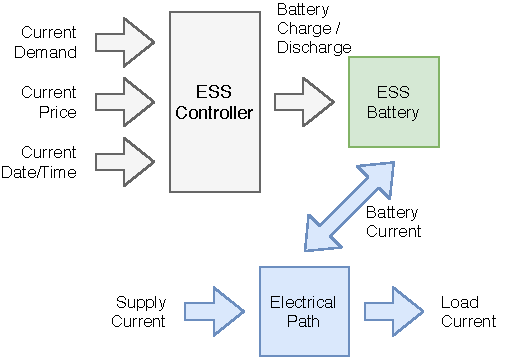
\includegraphics[scale=0.68]{Content/fig/ess_components}
	\caption{Example \ac{ESS} Components\label{fig:ess-components}}
\end{figure}

\acp{ESS} work by shifting the burden of their electrical load to the
electrical grid during periods of low demand, i.e. when the price is the cheapest.
Then, as the load on the grid increases along with consequent increase
in price, the \ac{ESS} starts to supply its load from its battery instead. 
This results in a lower average cost for providing the load current. 
This system must be functionally correct while also meeting timing
deadlines i.e.
the system must respond to safety situations within a time bound. 

Our \texttt{ESS} has an associated
over-current detector.  When this triggers, the system must evade this
unsafe situation within 30 milli-seconds to activate a circuit
breaker, which must take effect within this deadline. 
However, the response time of the overall \texttt{ESS} controller is much less strict, as it has a soft-real time \textit{quality of service} deadline of one second.
This is primarily because the demand input of the \texttt{ESS} does not need to be sampled faster than every second for suitable behaviour.
In addition, the price of electricity changes only once every 10 minutes.
%  \pr{You may also
%  add the response time requirement upfront, which is from input to
%  the corresponding output of a given \ac{SANN}.}

\ignore{Deciding when to charge and discharge an \ac{ESS} battery is non-trivial. 
	There are many factors to consider, including the current \ac{SoC} of the battery, historical data on pricing and load demand current.
	A variety of approaches have been used, including statistical modelling in \cite{TOUESS}.
	%In addition, a system that is in charge of a battery must include
	%safety features, i.e. an electrical over-current detector, to ensure
	%that the users of the \ac{ESS} remain safe at all times: In the event
	%of an over-current, the industry standard requires that this unsafe
	%situation should be evaded within 30ms. 
}

We propose a meta neural network, involving three 3-layer \ac{MLP} \acp{SANN}, to decide when to charge and discharge the battery in our \texttt{ESS}.
These networks operate synchronously with a over-current detector
that preempts the system by activating a circuit breaker.
The architecture of this meta neural network is presented in Figure~\ref{fig:ess-sanns}. 
%In this case, 
%Using the ``layer by layer'' approach, we can guarantee a low \ac{WCRT} to ensure safety in the face of an electrical over-current, 
%as the \textit{Safety Cutoff} heuristic will be evaluated in each synchronous tick.

\begin{figure}
	\centering
	\scalebox{0.7}{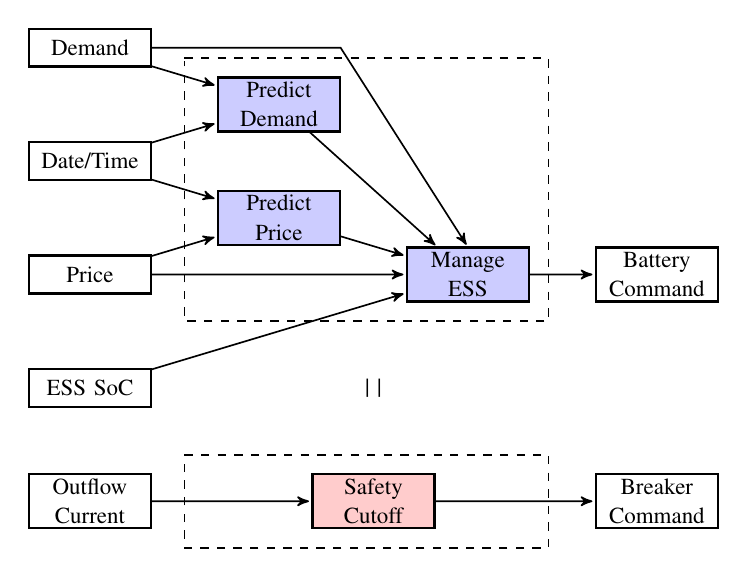
\begin{tikzpicture}[->,>=stealth',shorten >=1pt,auto,
node distance=3cm,
semithick,scale=0.8, transform shape,scale=0.6, font=\huge]

\tikzstyle{every state}=[rectangle, text width=3cm, minimum height=1cm, text centered, 
fill=blue!20,draw=none,text=black, draw,line width=0.3mm, font=\LARGE]

%start state
\node[state,fill=none]
(cdemand)
{Demand}; 

\node[state,fill=none]
(ctime) [below of=cdemand]
{Date/Time};

\node[state,fill=none]
(cprice) [below of=ctime]
{Price}; 

\node[state,fill=none]
(csoc) [below of=cprice]
{ESS SoC}; 

\node[state,fill=none]
(ccur) [below of=csoc]
{Outflow Current}; 

\node[state]
(prdemand) [right of=cdemand, xshift=2cm, yshift=-1.5cm]
{Predict Demand}; 

\node[state]
(prprice) [below of=prdemand]
{Predict Price}; 

\node[state]
(ess) [right of=prprice, xshift=2cm, yshift=-1.5cm]
{Manage ESS};

\node[state,fill=red!20]
(scut) [right of=ccur, xshift=4.5cm]
{Safety Cutoff}; 

\node[state,draw=none, fill=none]
(parallel) [above of=scut]
{\texttt{||}}; 

\node[state,fill=none]
(essoutp) [right of=ess, xshift=2cm]
{Battery Command};

\node[state,fill=none]
(breaker) [right of=scut, xshift=4.5cm]
{Breaker Command};

\path[->] (cdemand) edge (prdemand);
\path[->] (ctime) edge (prdemand);
\path[->] (ctime) edge (prprice);
\path[->] (cprice) edge (prprice);
\path[->] (cprice) edge (ess);
\path[->] (prdemand) edge (ess);
\path[->] (prprice) edge (ess);
\path[->] (csoc) edge (ess);
\path[->] (ess) edge (essoutp);
\path[->] (ccur) edge (scut);
\path[->] (scut) edge (breaker);

\draw[->] (cdemand.east)  
	|- ($(cdemand.east) + (5cm, 0)$) 
	-\ (ess.north);
	
\draw[-,dashed] ($(prdemand.north) + (-2.5cm, 0.5cm)$) 
-| ($(ess.east) + (0.5cm, 0)$) 
|- ($(ess.south) + (0, -0.5cm)$)
-| ($(prdemand.north) + (-2.5cm, 0.5cm)$);

\draw[-,dashed] ($(scut.north) + (-5cm, 0.5cm)$) 
-| ($(scut.east) + (3cm, 0)$) 
|- ($(scut.south) + (0, -0.5cm)$)
-| ($(scut.north) + (-5cm, 0.5cm)$);

\end{tikzpicture}
}
	\caption{ESS \ac{SANN} / Safety Cutoff arrangement}
	\label{fig:ess-sanns}
\end{figure}

Training this system complex, as it is not
feasible to provide all possible correct commands for every possible
input. Hence, back-propagation could not be used.
Instead, Q-learning~\cite{qlearning2010}, a type of reinforcement learning, was used for training the network.
\ignore{ Reinforcement learning trains an \ac{ANN} without knowledge of the
	correct output. 
	
	It trains based on the reinforcement of the reward of any given action $A$, with regard to the current state $S$. 
	An action that is \emph{good} will be given a high reward, and the \ac{SANN} will get its weights updated in an attempt to preserve the behaviour.
	A \emph{bad} action, however, will result in the  weights being modified so that it will have a reduced chance of choosing that action in that state again. 
	Using this system, Q-learning attempts to train an \ac{SANN} to follow the path of highest reward.}


%In our case, demand and price were modelled as sine functions, and the networks were trained with the goal of reducing the overall ``real-world'' cost \pr{I don't understand what you mean here?}
%of outputting energy from the \ac{ESS} system. 
%The \ac{ESS} was rewarded for buying energy when it was cheap, and supplying it when it was expensive.

In order to validate this design, we performed \ac{WCRT} analysis of
both the mono-periodic and multi-periodic implementations. 
%\pr{What
%  was the length of the multi period? For all these benchmarks, we
%  have to state the length of the period and the how many cycles are
%  needed. In particular, we have to state from input to output how
%  long it takes for all approaches.}
These results are presented in Table~\ref{tbl:res-ess}.

\begin{table}[H]
	\centering
	\caption{\ac{WCRT} results for \texttt{ESS}}
	\label{tbl:res-ess}
	\begin{tabular}{|l|l|l|}
		\hline
		Approach         & WCRT (ms) & Response Time (ms)\\ \hline
		Black-box        & 14   & 14 \\ 
		Layer by layer   & 9.8  & 58.8 \\ \hline
	\end{tabular}
\end{table}

As can be seen, the \ac{WCRT} for the mono-periodic ``black-box''
approach is $14ms$, 
making the total worst-case cut-off time $28ms$ (one cycle to capture value, one cycle to emit command).
This only gives $2ms$ for the hardware to respond to a digital signal
to cut the circuit, which may not be sufficient.

Considering this, we developed  a multi-cyclic ``layer by layer''
approach, that results in a \ac{WCRT} of $9.8ms$, 
giving a total worst-case cut-off time time of $<20ms$. 
This gives sufficient time for the physical hardware to respond and break the circuit.
In addition, although changing the implementation to multi-cyclic does increase the \ac{ANN} response time by $54.8$ms, it does not
come close to the deadline of the \ac{ESS} battery command, which has a one second soft-real time deadline.

\paragraph{\texttt{AI-BRO}}
%\subsection{AI-BRO} 
Introduced in Section~\ref{sec:motivating-example}, and as depicted in Figure~\ref{fig:av}, \texttt{AI-BRO} uses three different \acp{SANN} working together to guide an automatic vehicle. 
For this case study, the \acp{SANN} were simple \acp{MLP}.
Each was trained using back-propagation with a gradient descent approach~\cite{yegnanarayana1994artificial}, as the correct outputs for each of the inputs could be exactly specified.
For instance, \texttt{AI-BRO}, a front sensor reading of $(010)_2$ implies an obstacle directly in front of the vehicle.
Therefore, the vehicle must either turn left, turn right, or stop.
%\changed{\sout{The front \ac{SANN} is responsible for passing this information to the driver \ac{SANN}.}}
Consequently, it should output $(101)_2$.
%The first network takes input from the frontal sensors. These consist of 3 boolean values.
%Then, it outputs an initial suggestion for the car to travel, as an enumerated value across 3 bits for 6 different actions \textit{\{stop, stop/turn left, stop/turn right, turn left, turn right, continue straight\}}.

%Like the first network, the second \ac{SANN} also processes sensor data. 
%This time, the inputs are boolean values coming from the side sensors.
%A single boolean output for each side indicates whether or not a given direction is obstructed.

%The third and final \ac{SANN} takes in the outputs from the two sensor-processing networks. 
%Using the information they provide, it makes the actual decision for the car to follow.


Once created, \ac{WCRT} values were able to be derived for both mono-cyclic and multi-cyclic implementations, and are provided in Table~\ref{tbl:res-aibro}.

\begin{table}[H]
	\centering
	\caption{\ac{WCRT} results for \texttt{AI-BRO}}
	\label{tbl:res-aibro}
	\begin{tabular}{|l|l|l|}
		\hline
		Approach         & WCRT (ms) & Response Time (ms)\\ \hline
		Black-box        & 2.8  & 2.8  \\ 
		Layer by layer   & 1.9  & 11.4 \\ 
		Neuron by neuron & 1.8  & 10.8 \\ \hline
	\end{tabular}
\end{table}


\paragraph{\texttt{XOR} / \texttt{ADDER}}
%\subsection{XOR / ADDER}
\label{sec:xor-and-adder}

In addition to the exclusive-or \ac{MLP} \texttt{XOR} used as an example in Sections
\ref{sec:esterel-mapping} and \ref{sec:concurrent-sann},
an \ac{MLP} \texttt{ADDER} was also created that could add two 31-bit numbers together. 
These two networks were both straightforward to train and analyse 
due to their simple 3-layer designs, and their \acp{WCRT} are presented in Table~\ref{tbl:res-xor-adder}.

\begin{table}[H]
	\centering
	\caption{\ac{WCRT} results for \texttt{XOR} and \texttt{ADDER}}
	\label{tbl:res-xor-adder}
	\begin{tabular}{|l|l|l|}
		\hline
		Approach         & WCRT (ms) & Response Time (ms)\\ \hline
		\multicolumn{3}{|l|}{\texttt{XOR}}  \\ \hline
		Black-box        & 0.82 & 0.82   \\ 
		Layer by layer   & 0.57 & 1.71  \\ 
		Neuron by neuron & 0.6  & 1.8 \\  \hline
		\multicolumn{3}{|l|}{\texttt{ADDER}}  \\ \hline
		Black-box        & 0.49 & 0.49   \\ 
		Layer by layer   & 0.39 & 1.17  \\ 
		Neuron by neuron & 0.33 & 0.99 \\  \hline
	\end{tabular}
\end{table}

\paragraph{\texttt{HELLO}}
%\subsection{HELLO}

The \texttt{HELLO} system is a 3-layer \ac{RNN} which was trained to learn the pattern of the word ``hello''. 
We implemented this system to demonstrate that the synchronous
approach works with any type of \acp{ANN}, not just \acp{MLP}.
The results of this system are presented in Table~\ref{tbl:res-hello}.

\begin{table}[H]
	\centering
	\caption{\ac{WCRT} results for \texttt{HELLO}}
	\label{tbl:res-hello}
	\begin{tabular}{|l|l|l|}
		\hline
		Approach         & WCRT (ms) & Response Time (ms)\\ \hline
		Black-box        & 2.22  & 2.22  \\ 
		Layer by layer   & 1.33  & 3.99  \\ \hline
	\end{tabular}
\end{table}


\paragraph{\texttt{RABBIT} and \texttt{SENSOR}}
%\subsection{RABBIT}

%\pr{Is this a well known game? Citation needed}.


\ignore{The game is played in turns between two teams: wolves and a rabbit who
	are moving in a map. The wolves play on the same turn, working
	together to catch the rabbit. 
	The rabbit plays alone and attempts to escape the map. The wolves play on the same turn, working together to
	catch the rabbit. The rabbit scores if it leaves the map before time
	runs out. The wolves, on the other hand, win if they catch the
	rabbit before time runs out. The game runs in a loop. At the
	start of every round, all animals decide \textit{at the same time}
	where they will move too. 
	The system then updates and computes the score accordingly. Unless
	there was a winner, or time ran out, the 
	iterations continue.}

The \texttt{RABBIT} game was designed to highlight the benefits of synchronous
programming while designing meta neural networks. 
The game is played in turns between two teams, wolves and a rabbit, who
are moving in a map.
Each animal in the game has its own functional \ac{ANN}, which operate synchronously, respecting causality and avoiding deadlocks. 
The same system was also implemented in Python (using
Pthreads), without the use of any synchronization primitives, and we found
that the %\changed{\sout{
%We used
%these examples to evaluate the correlation coefficient between the
%Python and the Esterel implementation and found that the }
outputs of the two versions were
strongly correlated. %}

\ignore{The \acp{ANN} were run concurrently on separate Pthreads and the system updated after each \ac{ANN} thread finished running. 
	Although uncommon, it was noted that the Pthread implementation was
	susceptible to producing scores that should have been impossible
	for the system to attain. For example, the rabbits and wolves scoring on the same turn; this should not be possible, as either the wolves win or the rabbit, but not both. This was due to the disregard for causality in the
	running of Python's threads. \pr{I am unclear what you are claiming
		here. What is an impossible score and why? Are you referring to
		typical race conditions?}
	
	%Unfortunately this system is not currently time analysable using Platin. The system was originally implemented without regard to the timing analysis guidelines of \acp{SANN} as listed in Section~\ref{sec:wcrt}. As a result, this system contains some code that prevents WCET analysis at this time.
	
	Due to the large number of neurons in the \acp{ANN} of this system, one of the wolf \ac{ANN} was used to calculate the correlation coefficient between an Esterel implementation of an \ac{ANN}, i.e. \ac{SANN}, and an asynchronous \ac{ANN} using the exact same weights.
	
	The results of these calculations are presented in Table~\ref{tbl:res-game}.
	\begin{table}[H]
		\centering
		\caption{Correlation coefficient results for \texttt{RABBIT}}
		\label{tbl:res-game}
		\begin{tabular}{|l|l|}
			\hline
			Coefficient & Value \\
			\hline
			Pearson & 0.999999802345 \\
			\hline
		\end{tabular}
	\end{table}
	
	\paragraph{SENSOR}
	%\subsection{SENSOR}
}


\acp{DNN} have many industrial applications compared to any other type
of \ac{ANN}. This is largely due to their ability to train to
extremely large amounts of data. We implemented a \texttt{SENSOR}
application using a \ac{DNN}. An open source library called Darknet~\cite{redmon2015real} was used
to implement this \ac{CNN}. Darknet provides a platform for training
of many types of \acp{ANN} in C, including \acp{CNN}. 
%\changed{\sout{Using an already trained \ac{CNN} that can perform object recognition
%on input images, an Esterel system was created to run this \ac{CNN}, using the
%mentioned blackbox approach and the layer--by--layer approach.}
Using this system, an Esterel application was developed to recognize images using the black-box and the layer by layer approaches.%}

\begin{table}[H]
	\centering
	\caption{MNN2C Static \ac{WCRT} results for \texttt{ESS}, \texttt{AI-BRO}, \texttt{XOR} and \texttt{ADDER}}
	\label{tbl:res-mnn2c}
	\begin{tabular}{|p{0.15\textwidth}|p{0.15\textwidth}|p{0.15\textwidth}|p{0.15\textwidth}|p{0.15\textwidth}|p{0.15\textwidth}|}
		\hline
		Benchmark         & Original Black-box WCRT (ms) & MNN2C Black-box WCRT (ms)  &  \% decrease & MNN2C Multicore WCRT (ms) & \% decrease\\ \hline
		\texttt{ESS}        & 14 & 4.41 & 68.5 & 2.43 & 82.64 \\  \hline
		\texttt{AI-BRO}        & 2.8 & 2.29 & 18.21 & 1.47 & 47.5 \\ \hline
		\texttt{XOR}        & 0.82 & 0.53 & 35.37 & 0.53 & 35.37 \\  \hline
		\texttt{ADDER}        & 0.49 & 0.37 & 24.49 & 0.37 & 24.49 \\ \hline
	\end{tabular}
\end{table}

\begin{table}[H]
	\centering
	\caption{Combined \ac{WCRT} results for \texttt{ESS}, \texttt{AI-BRO}, \texttt{XOR}, \texttt{ADDER} and \texttt{HELLO}}
	\label{tbl:res-sann}
	\begin{tabular}{|l|l|l|l|}
		\hline
		Approach         & WCRT (ms) & Response Time (ms) & Size (neurons) \\ \hline
		\multicolumn{4}{|l|}{\texttt{ESS}} \\ \hline
		Black-box        & 14  & 14 & 125 \\ 
		Layer by layer   & 9.8  & 58.8 & 125 \\
		MNN2C			 & 4.41 & 4.41 & 125 \\ \hline
		\multicolumn{4}{|l|}{\texttt{AI-BRO}}  \\ \hline
		Black-box        & 2.8  & 2.8 & 35 \\ 
		Layer by layer   & 1.9  & 11.4 & 35 \\ 
		Neuron by neuron & 1.8  & 10.8 & 35 \\ 
		MNN2C			 & 2.29 & 2.29 & 35 \\ \hline
		\multicolumn{4}{|l|}{\texttt{XOR}}  \\ \hline
		Black-box        & 0.82 & 0.82 & 6  \\ 
		Layer by layer   & 0.57 & 1.71 & 6 \\ 
		Neuron by neuron & 0.6  & 1.8 & 6 \\ 
		MNN2C			 & 0.53 & 0.53 & 6 \\ \hline
		\multicolumn{4}{|l|}{\texttt{ADDER}}  \\ \hline
		Black-box        & 0.49 & 0.49 & 5  \\ 
		Layer by layer   & 0.39 & 1.17 & 5 \\ 
		Neuron by neuron & 0.33 & 0.99 & 5 \\ 
		MNN2C			 & 0.37 & 0.37 & 5 \\ \hline
		\multicolumn{4}{|l|}{\texttt{HELLO}}  \\ \hline
		Black-box        & 2.22  & 2.22 & 14 \\ 
		Layer by layer   & 1.33  & 3.99 & 14 \\ \hline
	\end{tabular}
\end{table}

\ignore{
	\pr{How
		many layers? Can we give some measurement-based timing analysis
		results for the game and the CNN?}
	The system ran through 16 layers, taking approximately 500ms for all 16 layers to run. This time was taken by measurement and is not a WCET value. Although no WCET analysis was possible, due to the open source library not following any of the timing analysis guidelines listed in Section~\ref{sec:wcrt}, the system was able to run in Esterel. This shows that the synchronous implementation of \acp{DNN} using C and Esterel is not only possible, but that the whole range of \acp{ANN} can be implemented synchronously using the Esterel programming language.
}














\section{Summary}
This chapter introduced the concept of \acfp{SNN} and their timing properties.

In Section~\ref{sec:motivating-example}, \acp{SNN} and their behaviour are introduced. 
Additionally, a motivating example is given with it's Esterel implementation.

Section~\ref{sec:wcrt} introduces the methods by which timing analysis is done on \acp{SNN} and the algebra involved with this.
This chapter also gives the first formal definition of a \ac{SNN} and discusses the periodicity of these \acp{SNN}.

The next section, Section~\ref{sec:concurrent-sann}, introduces the concept of \acfp{MNN} and provides formal definitions for them, as well as providing examples of the structure of the introduces \acp{MNN}.

A new Python compiler for creating \acp{MNN} from Keras is introduced in Section~\ref{sec:mnn2c} and its results are presented.

The final section of this chapter presents the results of the work done on \acp{SNN} and \acp{MNN} for this chapter.
These results are discussed and analysed, with conclusions drawn in the following chapter.

\section{Discussion}
\label{sec:conclusion}

In this work, we have presented an approach for synchronous composition of \acf{RE} with \acfp{ANN} for \acp{CPS} by defining \acfp{SNN}.
Our \acp{SNN} demonstrate that policies specifying safe I/O behaviours for \acp{ANN} can be enforced.
These enforced policies are shown to increase the safety and efficiency of the systems within which they are placed, without adding a large overhead to the system and without decreasing the functionality of the system.
In the three case studies presented, the \ac{RE} added an average overhead of just 6.035\%, but the efficiency and safety of each system was increased by an amount that rendered the overhead negligible.






\chapter{Runtime Verification of Synchronous Neural Networks}

% TODO:
% Show the effect of the RE when the system is trained to different degrees

\section{Verification of Deep Artificial Neural Networks}
Deep \acfp{ANN}~\cite{schmidhuber2015deep}, \acp{ANN} with large, complex inputs and a large, complex layer structure and multiple layers, are hard to verify due to their complex nature~\cite{Gehr2018AI2SA}. 
Lots of work has been put into the verification of \acp{ANN}, but the results yielded from this work have many limitations and are generally time consuming.

Previously, this thesis introduced the concept of using runtime enforcement to dynamically ``verify'' an \ac{ANN} as it runs. 
While this works very well for simple, feed forward \acp{ANN}, this does not extend to more complicated \acp{CNN}.

\subsection{Runtime Enforcement of Deep Artificial Neural Networks}
Runtime Enforcement, as a solution to the verification of \acp{ANN} and introduced in the previous chapter, only works when the inputs to the \ac{ANN} are known.
This works very well with feed forward \acp{ANN}, as their inputs are, generally, defined and known.
Take the AI-BRO \ac{ANN} discussed in Section~\ref{link-to-aibro}; this \ac{ANN} has a vector of defined inputs representing the objects ``seen'' by the vehicle.
Since dangerous situations are defined by both inputs and outputs, the outputs of this \ac{ANN} can be enforced because both the inputs and outputs are known at all times.

Complex \ac{ANN} inputs (such as images for \acp{CNN}) are unknown, and the purpose of the \acp{ANN} is to classify said inputs.
Since the inputs cannot be defined as something recognisable, the decision made by the \ac{ANN} cannot be classified as dangerous because a dangerous situation is defined by known inputs and outputs.
Take a \ac{CNN} that classifies pedestrians; we are using the \ac{CNN} because the software cannot recognise whether the input image shows a pedestrian or not.
If the pedestrian is misclassified as a tree, the system has no way to know this based off of the inputs to the \ac{CNN} alone.
Thus, behaviour of \acp{ANN} with complex inputs (most commonly classification \acp{ANN}) cannot be enforced using only the inputs to the \ac{ANN}.

The solution proposed is to use runtime enforcement as a means to safely combine the outputs from various sensors in the system and use these to enforce the outputs of the \ac{ANN}.


\subsection{Input Perturbation for Deep Artificial Neural Networks}
This chapter also tackles another problematic aspect of using \acp{CNN}: input perturbations.
A group showed that very slight modifications to the input image of a \acf{CNN}, such as the discolouration of a few pixels, could cause the image to be misclassified~\cite{Gehr2018AI2SA, ann-pert}.
A \ac{CNN} can train to high accuracy, e.g. 99.99\%, on the training set, but simple perturbations to the \ac{CNN}'s input can lead to drastically reduced accuracy once the \ac{CNN} has been deployed.
This thesis shows two methods of increasing the prediction accuracy of an \ac{CNN} affected by input perturbations: the first is the above-mentioned sensor fusion with runtime enforcement and the other is using a \acf{MNN} ensemble of different \acp{CNN}, each classifying a different aspect of the input image and congregating to make a decision as a whole.


\subsection{Sensor Fusion and Runtime Verification for Deep Artificial Neural Networks}
Sensor fusion is a highly researched topic for increasing the accuracy of object detection \acp{CNN}~\cite{SensorFusion2017}. 
Sensor fusion is the combination of two or more different sensor types to increase the overall sensor detection accuracy of the system.
Where \acfp{AV} are concerned safety is of utmost importance, making this the biggest area of research for sensor fusion using \acp{CNN}.

The proposed approach to safe deep \acp{ANN} combines runtime enforcement and sensor fusion to safely increase the detection accuracy of \acp{CNN} in \acp{AV}.
The sensors in question are a 360$\circ$ \ac{LiDAR} sensor and three front-facing cameras.
The sensor outputs are combined synchronously using a synchronous runtime enforcer, however the runtime enforcer does not enforce the outputs of the detection system.
Rather, the runtime enforcer verifies the integrity of the detected outputs, and in the case of a possible misclassification the system is put into a safe mode where control of the vehicle is returned to the driver.
This type of runtime enforcement has been termed as ``runtime verification''.
Using a \acf{SSNN} as the \ac{CNN} in the \ac{AV} system, the system is kept synchronous, time predictable and easy to formalise.

Additionally, to reduce the impact of perturbations to the \ac{CNN}'s inputs, the \ac{SSNN} used in the system is actually a \ac{MNN} composed of three \ac{MNN} ensembles, each with three synchronous \acp{CNN}.
This \ac{MNN} aims to greatly increase the prediction accuracy by splitting the prediction process amongst multiple, different \acp{CNN} such that the weakness of each \ac{CNN} is addressed by the other \acp{CNN}.















\section{Multi-Periodic \acp{SNN} in Esterel}
\label{sec:esterel-mapping}

The mono-periodic implementation of \ac{SNN} using the methodology in Listing~\ref{lst:ai-bro}, while being time predictable, has limitations.
This is because each \ac{NN} must run to completion before any reaction can complete. 
For large networks with many hidden layers, this is not ideal --- as
the overall \ac{WCRT} of the system could become quite large, causing
violations when considering response to some critical inputs which may
need immediate attention to ensure safety. We highlight this aspect
using an \acf{ESS} case study in Section~\ref{sec:results}.

There are other approaches for arranging the internals of each network while still meeting Definition~\ref{def:sann}, and to illustrate this, we will use a simple XOR (exclusive or) \ac{MLP}.
This network is depicted in Figure~\ref{fig:xor-ann}, and as can be seen, it features five neurons in three layers. While we use this simple illustration, the 
methodology is applicable for any \ac{NN}.

\begin{figure}[h]
	\centering
	\scalebox{0.8}{\def\layersep{2.25cm}
\begin{tikzpicture}[shorten >=1pt,->,draw=black!100, node distance=\layersep]
	\tikzstyle{every pin edge}=[<-,shorten <=1pt]
	\tikzstyle{neuron}=[circle,fill=black!25,minimum size=20pt,inner sep=0pt]
	\tikzstyle{input neuron}=[neuron, fill=white!100,draw=black];
	\tikzstyle{output neuron}=[neuron, fill=white!100,draw=black];
	\tikzstyle{hidden neuron}=[neuron, fill=white!100,draw=black];
	\tikzstyle{annot} = [text width=4em, text centered]
	
	% Draw the input layer nodes
	\foreach \name / \y in {1,...,2}
	% This is the same as writing \foreach \name / \y in {1/1,2/2,3/3,4/4}
	\node[input neuron, pin=left:Input $x_\y$] (I-\name) at (0,-\y) {$i_\y$};
	
	% Draw the hidden layer nodes
	\foreach \name / \y in {1,...,3}
	\path[yshift=0.5cm]
	node[hidden neuron] (H-\name) at (\layersep,-\y cm) {$h_\y$};
	
	% Draw the output layer node
	\node[output neuron,pin={[pin edge={->}]right:Output $y$}, right of=H-2] (O1) {$o_1$};
	
	% Connect every node in the input layer with every node in the
	% hidden layer.
	%\foreach \source in {1,...,2}
	%\foreach \dest in {1,...,3}
	%\path (I-\source) edge node[above] {1} (H-\dest);
	\path (I-1) edge node[above] {1} (H-1);
	\path (I-1) edge node[above] {0.5} (H-2);
	\path (I-2) edge node[above] {0.5} (H-2);
	\path (I-2) edge node[above] {1} (H-3);
	
	% Connect every node in the hidden layer with the output layer
	%\foreach \source in {1,...,3}
	\path (H-1) edge node[above] {1} (O1);
	\path (H-2) edge node[above] {-2} (O1);
	\path (H-3) edge node[above] {1} (O1);
	
	% Annotate the layers
	\node[annot,above of=H-1, node distance=2cm] (hl) {\textit{Hidden Layer}\\$l_h$};
	\node[annot,left of=hl] {\textit{Input Layer}\\$l_i$};
	\node[annot,right of=hl] {\textit{Output Layer}\\$l_o$};
\end{tikzpicture}}
	\caption{Example of an XOR \ac{ANN} showing its layers and weights.	\label{fig:xor-ann}}
\end{figure}

Each neuron in this network is based on the model in Figure~\ref{fig:artificial-neuron}, with a simple Boolean step activation function and zero bias. 
The activation function is represented by Equation~\ref{eqn:xor-neuron}, where $y$ is the output, $x \in X$ are the inputs, and $w \in W$ the weights.

\begin{equation}
y =
\begin{cases}
1 & \text{$\Sigma_{i} \left(x_i \times w_i\right) >= 1$} \\
0 & \text{otherwise}
\end{cases}
\label{eqn:xor-neuron}
\end{equation}

\begin{definition}
	\label{def:bb-mlp}
	An \ac{MLP} is formalised as a tuple $M = \langle I, O, N, L,
	\alpha, \eta  \rangle$, where:
	\begin{itemize}
		\item $I$ is a finite collection of input variables with
		its domain being $\mathbf{I} = \mathbb{R}^n$
		\item  $O$ is a finite collection of  output variables with
		its domain being $\mathbf{O} = \mathbb{R}^m$
		\item  $N$ denotes a set of neurons
		\item $L$ denotes a set of layers
		\item $\alpha: N \rightarrow L$ is the neuron mapping function
		that maps a given neuron to a layer
		\item $\eta: \mathbf{I} \rightarrow \mathbf{O}$ is the non-linear
		function (termed the network function) that provides the behaviour of a given network i.e.
		when provided a vector of input of size $n$ produces an
		vector of output of size $m$. Internally, 
	\end{itemize}
	\ignore{
		$i \in I$ is each input to the network, $o \in O$ is each output from the network, 
		$\eta$ is the set of neurons, $L$ is the set of layer functions $l:i \rightarrow o$ which perform intermediate data transforms, $m: \eta \rightarrow L$ is the neuron mapping function that associates a neuron to a given layer,
		and $f: I \rightarrow O$ is a function that captures the non-linear behaviour of the entire network 
		--- i.e. a ``black-box'' untimed non-linear transformation function which converts inputs to outputs via the execution of each layer of neurons in sequence.}
	%$m \subset \eta \times L$ provides the mapping of neurons to layers. 
	%	We can describe the operation of $n$ as $n\left(I\right) = O$, i.e. $n$ describes a `black-box' untimed non-linear transformation function which converts inputs to outputs via the execution of each layer of neurons.
\end{definition} 

\begin{example}
	The \ac{MLP} presented in Figure~\ref{fig:xor-ann} can be presented formally as $I=\langle x_1, x_2 \rangle$, $O = \langle y \rangle$, $N= \{i_1, i_2, h_1, h_2, h_3, o_1\}$ and $L
	= \{l_i, l_h, l_o\}$. The function $\alpha$ maps neurons to
	layers e.g. $\alpha(h_1) = l_1$ and the network function $\eta$
	given input $\langle 0, 1 \rangle$ produces an output $1$
	i.e. $\eta(\langle 0, 1 \rangle) = 1$.
	
\end{example}
%\pr{Illustrate this definition using Figure~\ref{fig:xor-ann}. Also, where is this definition used formally?}

Using Definition~\ref{def:bb-mlp}, we can implement the XOR \ac{ANN} as a ``black-box'' function in Esterel, as presented in Figure~\ref{fig:tca-bb-n}. 
The corresponding mono-periodic \ac{TCA} is shown beside the code.
The \ac{WCRT} is the time taken to execute the network function
$\eta$, i.e. $WCRT\left(M\right) = WCRT\left( \eta\right)$. 
In the following, we use $WCRT(\eta)$ and $\eta$ interchangeably.

\begin{figure}[h]
	\centering
	\begin{subfigure}[h]{0.15\textwidth}
		\centering
		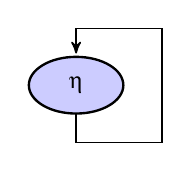
\begin{tikzpicture}[->,>=stealth',shorten >=1pt,auto,
node distance=2.5cm,
semithick,scale=0.8, transform shape,scale=0.6]

\tikzstyle{every state}=[ellipse, minimum width=2.5cm, minimum height=1.5cm, text centered, 
fill=blue!20,draw=none,text=black, draw,line width=0.3mm, font=\LARGE]

%start state
\node[state]
(init) 
{$\eta$}; 

\draw[->] (init.south) 
|- ($(init.south) + (0, -0.75cm)$) 
-| ($(init.east) + (1cm, 0)$) 
|- ($(init.east) + (0, 1.5cm)$) 
-| (init.north);

\end{tikzpicture}

	\end{subfigure}%
	\begin{subfigure}[h]{0.33\textwidth}
		\vspace{3mm}
		\begin{lstlisting}
		loop
		emit y(run_XOR_ANN_n(?x1, ?x2));
		pause;
		end
		\end{lstlisting}
	\end{subfigure}
	\caption{Mono-periodic `black-box' execution, $WCRT = \eta$}
	\label{fig:tca-bb-n}
\end{figure}

It can be noted that by Proposition~\ref{lemma1}, any \ac{ANN} implemented using the approach in Figure~\ref{fig:tca-bb-n} is also an instance of \ac{SNN} defined using Definition~\ref{def:sann}.
%\pr{This is same as the lemma in section 2. Do we need this?}

\begin{theorem}
	\label{thm:bb-soundness}
	(Soundness) A mono-periodic \ac{SNN} given an input vector $\mathbf{i}$
	produces an output vector $\mathbf{o}$ in a given tick \miff the corresponding \ac{MLP} 
	given the same input vector $\mathbf{i}$ produces the identical output vector $\mathbf{o}$ during any execution.
	
	%The synchronous execution of a ``black-box'' function $n$ will give the same output values $O$ for the same input values $I$ as the non-synchronous execution of the
	%\ac{MLP} $n$.
\end{theorem}

\begin{proof}
	The proof of Theorem~\ref{thm:bb-soundness} trivially follows from the
	fact that synchronous execution of a black-box function does not change
	the mathematical properties of that function. %, as all Esterel function
	%calls are state-less and  side effect free.
\end{proof}

\ignore{
	
	\begin{equation}
	y = f\Big(b + \sum_{i=1}^{n} \left(x_i \times w_i\right)\Big)
	\label{eqn:artificial-neuron}
	\end{equation}
	
	In the XOR example, each neuron has a \textit{threshold step function} as its activation function $f$, and has zero bias $b$.
	Hence, each neuron in the \textit{hidden} and \textit{output} layers is following Equation~\ref{eqn:xor-neuron}.
	
	\begin{example}
		In our XOR \ac{ANN}, let $i_1 = 1$ and $i_2 = 0$. \\
		Then, as $1 \times 1 \geqslant 1$, $h_1y = 1$. \\
		However, $\big(\left(1 \times 0.5\right) + \left(0 \times 0.5\right)\big) \ngeqslant 1$, so $h_2y = 0$.
		Likewise, $h_3y = 0$.  \\
		Then, as $\big((1 \times 1) + (0 \times -2) + (1 \times 1)\big) \ngeqslant 1$, the final output $o_1y = 1$.  \\
		This is correct, as $1$ \textit{xor} $0 = 1$.
	\end{example}
}

\begin{figure}[h]
	\centering
	\begin{subfigure}[h]{0.6\textwidth}
		\centering
		\begin{subfigure}[h]{0.3\textwidth}
			\centering
			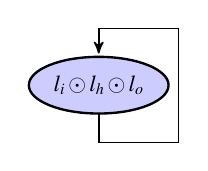
\begin{tikzpicture}[->,>=stealth',shorten >=1pt,auto,
node distance=2.5cm,
semithick,scale=0.8, transform shape,scale=0.6, font=\huge]

\tikzstyle{every state}=[ellipse, minimum width=2cm, minimum height=1.5cm, text centered, 
fill=blue!20,draw=none,text=black, draw,line width=0.3mm, font=\LARGE]

%start state
\node[state]
(init) 
{$l_i \odot l_h \odot l_o$}; 

\draw[->] (init.south) 
|- ($(init.south) + (0, -0.75cm)$) 
-| ($(init.east) + (0.25cm, 0)$) 
|- ($(init.east) + (0, 1.5cm)$) 
-| (init.north);

\end{tikzpicture}

		\end{subfigure}%
		\begin{subfigure}[h]{0.66\textwidth}
			\vspace{3mm}
			\begin{lstlisting}
			loop
			call run_XOR_ANN_li()(?x1, ?x2);
			call run_XOR_ANN_lh();
			emit y(run_XOR_ANN_lo());
			pause;
			end
			\end{lstlisting}
		\end{subfigure}
	\end{subfigure}
\caption{Mono-periodic `layer by layer' execution, $WCRT = l_i \odot l_h \odot l_o$}
\label{fig:tca-bb}
\end{figure}

\begin{figure}[h]	
	\centering
	\vspace{5mm}
	\begin{subfigure}[h]{0.5\textwidth}
		\centering
		\begin{subfigure}[h]{0.3\textwidth}
			\centering
			\begin{tikzpicture}[->,>=stealth',shorten >=1pt,auto,
node distance=2.5cm,
semithick,scale=0.8, transform shape,scale=0.6, font=\huge]

\tikzstyle{every state}=[ellipse, minimum width=2.5cm, minimum height=1.5cm, text centered, 
fill=blue!20,draw=none,text=black, draw,line width=0.3mm, font=\LARGE]

%start state
\node[state]
(l0) 
{$l_i$};

\node[state]
(l1) [below of=l0]
{$l_h$}; 

\node[state]
(l2) [below of=l1]
{$l_o$};  

\path[->] (l0) edge (l1);
\path[->] (l1) edge (l2);

\draw[->] (l2.south) 
|- ($(l2.south) + (0, -0.75cm)$) 
-| ($(l2.east) + (1cm, 0)$) 
|- ($(init.east) + (0, 1.5cm)$) 
-| (init.north);

\end{tikzpicture}

		\end{subfigure}%
		\begin{subfigure}[h]{0.66\textwidth}
			\begin{lstlisting}
			loop
			call run_XOR_ANN_li()(?x1, ?x2);
			pause;
			call run_XOR_ANN_lh();
			pause;
			emit y(run_XOR_ANN_lo());
			pause;
			end
			\end{lstlisting}
		\end{subfigure}
	\end{subfigure}
\caption{Multi-periodic `layer by layer' execution, $WCRT = l_i \oplus l_h \oplus l_o$}
\label{fig:tca-layers}
\end{figure}

\begin{figure}[h]
	\centering
	\vspace{5mm}
	\begin{subfigure}[h]{0.8\textwidth}
		\centering
		\begin{subfigure}[h]{0.3\textwidth}
			\centering
			\begin{tikzpicture}[->,>=stealth',shorten >=1pt,auto,
node distance=2.5cm,
semithick,scale=0.8, transform shape,scale=0.6, font=\huge]

\tikzstyle{every state}=[ellipse, minimum width=2.5cm, minimum height=1.5cm, text centered, 
fill=blue!20,draw=none,text=black, draw,line width=0.3mm, font=\LARGE]

%start state
\node[state]
(l0) 
{$i_1 \odot i_2$};

\node[state]
(l1) [below of=l0]
{$h_1 \odot h_2 \odot h_3$}; 

\node[state]
(l2) [below of=l1]
{$o_1$};  

\path[->] (l0) edge (l1);
\path[->] (l1) edge (l2);

\draw[->] (l2.south) 
|- ($(l2.south) + (0, -0.75cm)$) 
-| ($(l2.east) + (1.5cm, 0)$) 
|- ($(init.east) + (0, 1.5cm)$) 
-| (init.north);

\end{tikzpicture}

		\end{subfigure}%
		\begin{subfigure}[h]{0.66\textwidth}
			\begin{lstlisting}
			loop
			[
			call run_XOR_ANN_i1()(?x1);
			|| 
			call run_XOR_ANN_i2()(?x2);
			];
			pause;
			[
			call run_XOR_ANN_h1()();
			||
			call run_XOR_ANN_h2()();
			||
			call run_XOR_ANN_h3()();
			];
			pause;
			emit y(run_XOR_ANN_o1());
			pause;
			end
			\end{lstlisting}
		\end{subfigure}
	\end{subfigure}
\caption{Multi-periodic, neuron-by-neuron execution, $WCRT = \left(i_1 \odot i_2\right) \oplus \left(h_1 \odot h_2 \odot h_3\right) \oplus o_1$}
\label{fig:tcas-xor}
\end{figure}

As mentioned, using the approach in Figure~\ref{fig:tca-bb-n} to implement complex \acp{ANN} i.e. \acp{CNN} may lead to implementations that violate their timing requirements. 
The synchronous approach, however, enables efficient implementations via compositional modelling.
Esterel supports this via statements such as \texttt{pause} that help to create smaller ticks, \texttt{;} for indicating sequence operation, and \texttt{||}, which enables the modelling of concurrency. 

For example, the \ac{MLP} in Figure~\ref{fig:tca-bb-n} can also be
compositionally modelled by splitting the neural function $\eta$
into its constituent layers $l_i$, $l_h$, and $l_o$. 
While this maintains the overall functionality of the network, it
reduces the \ac{WCRT} by making the network multi-periodic, where each
period is shorter. 
As previously mentioned, the \ac{ESS} case study in Section~\ref{sec:results} examines the benefits of this approach.

%This has no major effect in Figure~\ref{fig:tca-bb}, where the network is still running in a single tick, as function $f$ will call these layers internally anyway.
%However, if \texttt{pause} statements are introduced between each layer, then the timing of the program changes significantly: 
%the \ac{WCRT} of the program will decrease, and the execution becomes `multi-cyclic'.
%Now, multiple \textit{ticks} are required to complete the execution of the neural network, but the program's responsiveness can be increased.

\begin{prop}
	%As long as a neural network's layers are still executed in
	%the correct order, the output will be correct after the last
	%layer is completed.
	The mono-periodic implementation of the XOR \ac{MLP} is functionally
	equivalent to the multi-periodic implementation.
\end{prop}

\begin{proof}
	For any input, output vectors $\mathbf{i, o}$ respectively, 
	$\eta\left(\mathbf{i}\right) = l_o\left(
	l_h\left( l_i\left( \mathbf{i} \right) \right) \right) =
	\mathbf{o}$
	%The proof of this follows intuitively as the operation of $\nu$ already recursively calls each layer $l \in L$ of neurons during execution --- we just remove one layer of indirection.
\end{proof}

\ignore{
	\begin{example}
		In the XOR \ac{MLP}, there are three layers $L = \{l_i, l_h, l_o\}$. 
		During execution, $\eta$ will invoke each layer in order as it executes each neuron. 
		We can make this explicit by calling layers as functions. 
		In this case, $\eta\left(i\right) = l_o\left(
		l_h\left( l_i\left( i \right) \right) \right) = o$
	\end{example} %\pr{While I agree that this result should hold, it is
	%unclear how function composition is actually happening in the
	%code. Code only provides a sequence of function calls without
	%showing the composition!}
}

\ignore{
	For example, a \ac{MLP} $n$ may be compositionally modelled using its constituent layers $l_i$, $l_h$, and $l_o$, as shown in Figure~\ref{fig:tca-bb} (b), (c) and (d).
	\pr{Explain each approach and the trade off. What is the distinction between approach (a) and (b)? Also, could we have just one theorem to 
		state that all approaches are equivalent i.e. they produce the same output albeit in different ticks.}
	
	\begin{lemma}
		A single-tick `layer by layer' execution of functions $l \in L$ the same output as executing function $n$ if all layers are executed in order.
	\end{lemma} 
}




\ignore{
	This has not reduced the \ac{WCRT} of the system, as $n$ has the same \ac{WCRT} as the sum of the three layers that make it up.
	However, if the layers are split over \emph{multiple ticks}, then the system \ac{WCRT} can reduce.
	
	An example of this multi-tick `layer by layer' approach is presented in Figure~\ref{fig:tca-layers}.
	
	\begin{lemma}
		A multi-tick `layer by layer' execution of layers $l \in L \in n$ will give the same output as executing network $n$ completely, iff all layers are executed in order and once a number of ticks equivalent to the number of layers has elapsed. I.e. the number of logical ticks $= |L|$.
	\end{lemma}
	The proof of this is \todo{?}
}

Observe that the response time of the multi-periodic implementation is
$3 \times T_2$, where $T_2$ is the \ac{WCRT} of the multi-periodic
version. In contrast, the response time as well as the reaction time
of the mono-periodic version is always its \ac{WCRT} $T_1$. However, it is
expected that $T_2 << T_1$.
%It is important to note that a multi-tick execution of an \ac{SNN} will not speed up the generation of outputs of the overall network --- as now, multiple ticks must be completed before a given output will be ready. 
%However, the length of each individual tick is reduced, which means that overall the system interactivity can be increased.

Like the breaking up of the function $\eta$ into its component
layers, we can also break each layer $l$ into its component neurons.
This option is presented in Figure~\ref{fig:tcas-xor}. 
Unlike in Figure~\ref{fig:tca-bb}, neurons are able to operate concurrently within each layer. 
This could provide benefits when considering multi-core
implementations such as in \cite{yuan2011compiling}.
\ignore{ however, for single-core single-threaded execution (the focus of this paper), this approach does not considerably alter tick length.} 

A summary of these approaches is presented in Table~\ref{tbl:sann-approaches}.
%we separated each neuron call with \texttt{pause} statements --- i.e. called each neuron in its own tick. 
\begin{table}[h]
	\centering
	\caption{Summary of \ac{SNN} approaches and their relevant figures, \ac{WCRT}, cycles and response time}
	\label{tbl:sann-approaches}
	\begin{tabular}{|l|l|l|l|l|}
		\hline
		Arrangement    & Figures & WCRT & Cycles & Response Time   \\ \hline
		Mono-periodic  & \ref{fig:tca-bb-n},\ref{fig:tca-bb} & High & 1 & == WCRT              \\
		Multi-periodic & \ref{fig:tca-layers},\ref{fig:tcas-xor}& Low  & \textgreater{}1 & \textgreater{}\textgreater{}WCRT \\ \hline
	\end{tabular}
\end{table}


\ignore{ 
	\pr{I suggest we use consistent terminology i.e. mono-cyclic TCA and multi-cyclic TCA and their corresponding Esterel implementation. Ideally, the proof of the theorem 
		can be done using induction. Consider a mono-cyclic implementation and multi-cyclic implementation of length $k$.
		Base case -- first time outputs after 1 tick and k ticks are same. Hypothesis -- outputs after $m$ executions are equivalent i.e. First network executed for 
		$m$ ticks while the second network executed for $k\ times m$ ticks and produced the same output starting from the same input. Proof: to show that this holds for $m+1$ executions.}
}

%\subsection{Implementing `Black-Box' \ac{SNN} in Esterel}

%The basic programming unit in Esterel is a \textit{module}. 
%Each module contains an interface declaration, followed by a body of executable statements.
%Variables are known as \textit{signals}, and may consist of a \textit{status} and a \textit{value} component. 
%Signals with only a status signals are denoted \textit{pure}, while those that contain values are instead denoted \textit{valued}.
%Sections of code may be separated with either the `\code{;}' or `\code{||}' operator, which denote sequencing and synchronous concurrency respectively.
%In order to perform manipulation of valued signals, Esterel can call external functions (provided in supplementary C files).

%Presented in Listing~\ref{lst:blackbox} and Listing~\ref{lst:blackbox-composition} are the simplest way of implementing neural networks in Esterel, already seen in the AI-BRO example.
%As can be seen, entire \acp{ANN} can be composed together and are simply called as external function calls, and will run each tick. 
%Networks can be composed together
%This can be considered the `bare minimum' to qualify as a \ac{SNN}, as the network is now running synchronously with its environment.

%Even though this implementation is quite trivial, it can still gives a strong advantage over a general-purpose implementation: when considering the methodology for composing multiple \acp{ANN}. 
%For example, consider a system that needs three \acp{ANN}, each performing a different task (as is the case in our AI-BRO example, in Section~\ref{sec:motivating-example}). 

%We can compose these multiple \acp{ANN} synchronously in Esterel. 
%As an example of this, consider an extension of our XOR network that computes $y = \big((x_1$ \textit{xor} $x_2)$ \textit{xor} $(x_3$ \textit{xor} $x_4)\big)$ (i.e. $y$ is $true$ when an odd number of inputs are $true$).
%We can compose this together still using the `black-box' methodology, as presented in Listing~\ref{lst:blackbox-composition}.
%Here, it can be seen that the first two \acp{ANN} can be run concurrently with one another, and the third \ac{ANN} can only be run when the first two are complete.



\section{Methodology} 
The system designed for this case study was made to reflect a \acf{AV} and its object detection mechanisms. 
The system used multiple techniques to tackle the inherent issues of the \ac{AV} system, i.e. weakness to perturbed inputs and misclassification detection.
The system's sensors include an overhead, 360$^\circ$ \acf{LiDAR} apparatus, and a single, frontal facing camera.
A solitary camera was sufficient to prove the efficacy of this solution, however it is to be noted that \ac{AV} systems generally use multiple cameras, facing different directions, so that the controller can make properly informed decisions.
The system used can be seen in Figure~\ref{fig:ssnn}. 

The \ac{LiDAR} for this system was accurate 93\% of the time~\cite{lidarFusion}, to closely simulate a real \ac{LiDAR} system.
The simulated camera outputs consisted of test images from both the \ac{VOC}~\cite{pascal-voc-2012} and \ac{GTSRB}~\cite{Stallkamp2012-gtsrb} datasets, in a combination of people, vehicles and various traffic signs.
The \ac{LiDAR} and camera outputs were handled by different parts of the controller.
The camera outputs were fed into a \ac{MNN} (see Figure~\ref{fig:mnn}) where they were classified by shape, colour and object type.

Utilising synchronous semantics, a \acf{MNN}, containing three other \ac{MNN} ensembles, was created.
Each ensemble synchronously combined the outputs of three different convolutional \acfp{SNN}~\cite{sann}, providing increased prediction accuracy for shape, colour and object type. 
These ensembles ran in synchronous concurrency, each taking four logical ticks to run. 
The outputs of each ensemble were then combined into batch of outputs forming the \textit{predicted output}. 

The system controller was encapsulated by a run-time enforcer~\cite{recps} that used sensor fusion to check for misclassifications made by the \ac{MNN}.
A safety automata (timed automata)~\ref{?} was designed to verify predictions made by the \ac{MNN} and ensure utmost safety at all times.
The automata started in a safe state, where control of the vehicle was autonomously handled by the system controller.
If a misclassification was detected, the enforced policy entered an unstable state, still under autonomous control. 
Once enough time passed without further misclassifications, the vehicle entered the safe state again.
However, if another misclassification was detected while unstable, the enforced policy entered a violation state and forced control of the \ac{AV} to the driver.
The vehicle would not enter autonomous mode again until the system was restarted.
A diagram of the enforced policy's safety (timed) automaton is shown in Figure~\ref{fig:signrte}.
This type of run-time enforcement, where neither the inputs nor outputs of the sensors or controller are enforced, has been termed as \textit{run-time verification}.
\textit{Run-time verification} refers to the verification of system parameters during run-time, while ensuring that the system is aware of any failed guards in the enforced policy.


\begin{figure}[t]
	\centering
	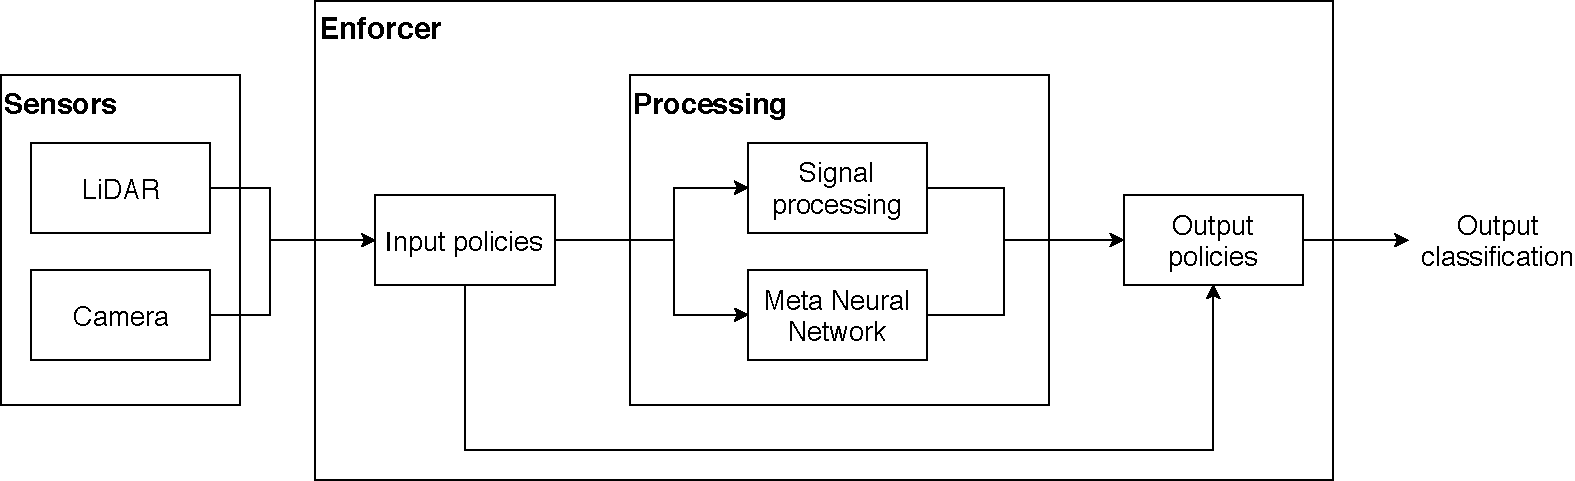
\includegraphics[scale=0.6]{Content/fig/SSNN.pdf}
	\caption{Block diagram showing the AV system with enforcer}
	\label{fig:ssnn}
\end{figure}

\begin{figure}[h]
	\centering
	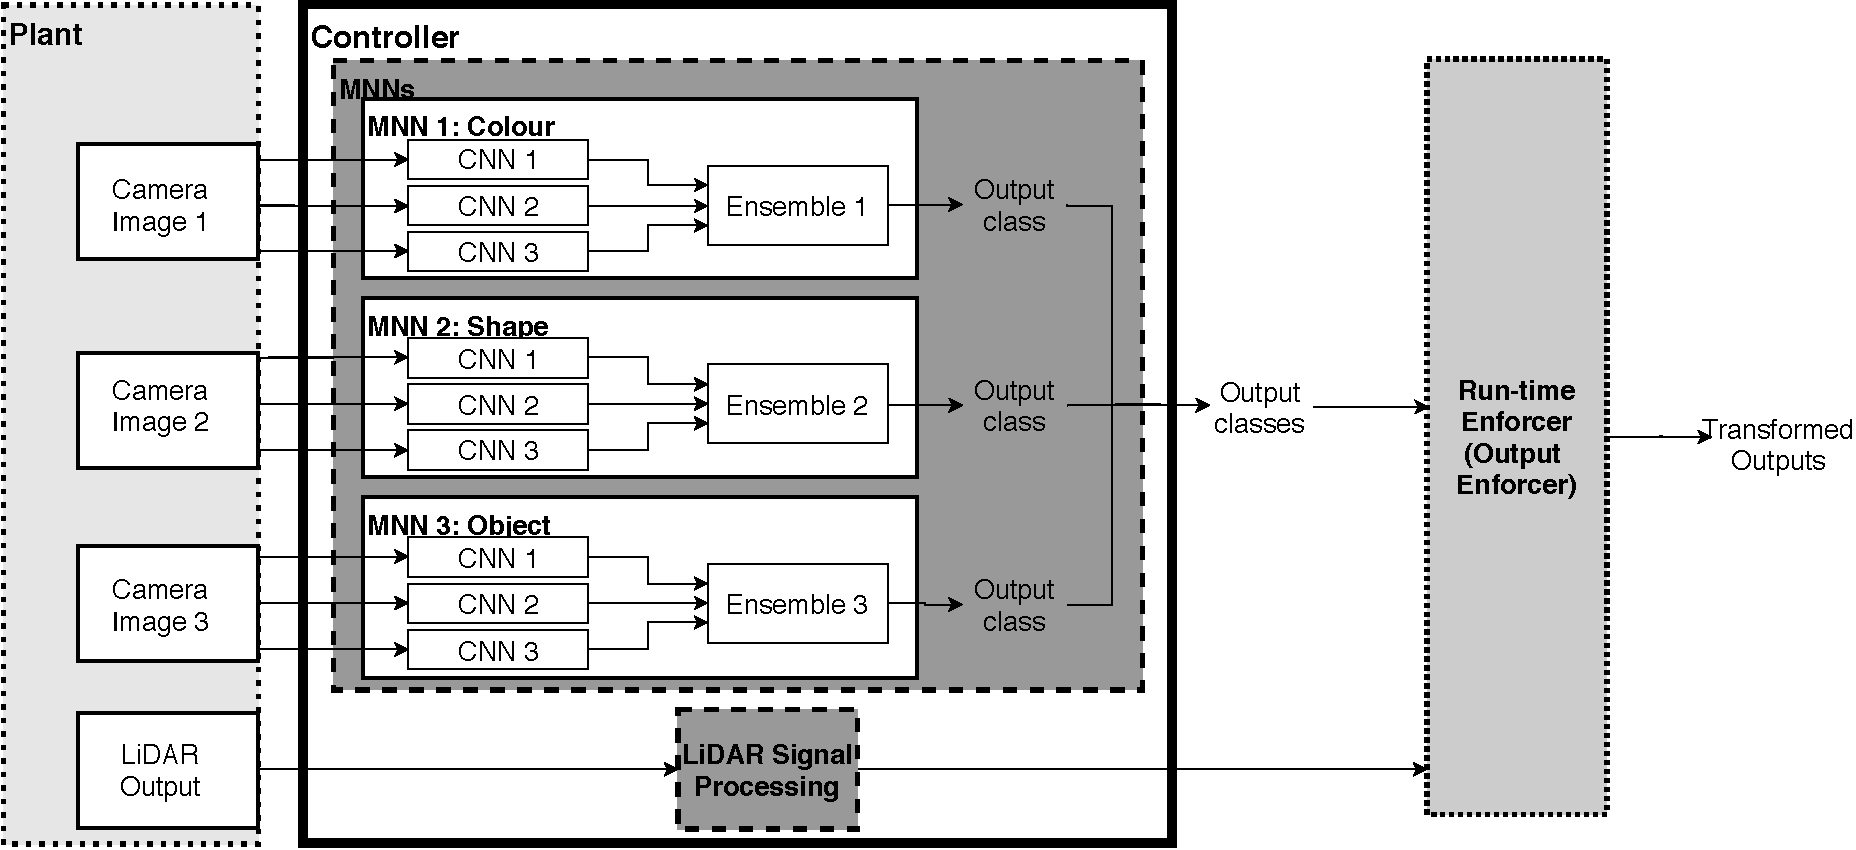
\includegraphics[scale=0.9]{Content/fig/MNN.pdf}
	\caption{Block diagram showing the Meta Neural Network ensemble} \label{fig:mnn}
\end{figure}

\begin{figure}[t]
	\centering
	\scalebox{1.3}{

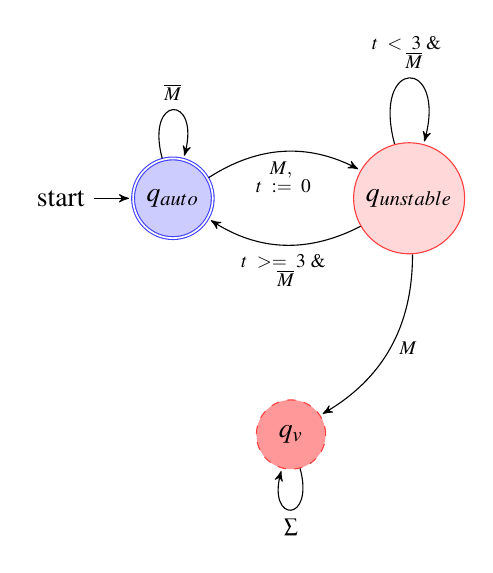
\begin{tikzpicture}[>=stealth',shorten >=1pt,auto,node distance=3 cm, scale = 1, transform shape]

\tikzstyle{accept} = [draw=blue!75,fill=blue!20]
\tikzstyle{violate} = [draw=red!75,fill=red!40, dashed]
\tikzstyle{unstable} = [draw=red!75,fill=red!15]

\node[initial,state, accepting, accept] (A) {$q_{auto}$};
\node[state, unstable] (B) [right of=A] {$q_{unstable}$};
\node[state, violate]         (C) [below of=B, xshift=-1.5cm]  {$q_v$};

\path[->] 
		(A) edge [loop above]       node [above]  
		{
			\scriptsize$\let\scriptstyle\textstyle\substack{\overline{M}}$
		} (A)
		
		(A) edge [bend left]		node [below]  
		{
			\scriptsize$\let\scriptstyle\textstyle\substack{
				M,~\\~
				t~:=~0~
			}$
		} (B)
	
		(B) edge [loop above]		node [above]  
		{
			\scriptsize$\let\scriptstyle\textstyle\substack{t~<~3~\&~\\~~\overline{M}}$
		} (B)
	
		(B) edge [bend left]		node [right]  
		{
			\scriptsize$\let\scriptstyle\textstyle\substack{M}$
		} (C)
	
		(B) edge [bend left]		node [below]  
		{
			\scriptsize$\let\scriptstyle\textstyle\substack{t~>=~3~\&\\~\overline{M}}$
		} (A)
	
		(C) edge [loop below] node [below]
		{
			\scriptsize$\sum$
		}(C)
		;

\end{tikzpicture}}

	\begin{itemize}
		\item $P$: Misclassification of a person.
		\item $V$: Misclassification of a vehicle.
		\item $N$: Classification of an object when there is nothing.
		\item $S$: Misclassification of a traffic sign.
		\item $C$: Confidence rating of the \ac{SNN} classification.
		\item $t$: Timer for the unstable state.
	\end{itemize}
	
	\caption{Enforcer policy for the AV prediction system}
	\label{fig:signrte}
\end{figure}


















\section{Results of the Runtime Verified AV System}

This research provides a solution for two aspects of \acf{AV} systems: predicting accurately with perturbations to the system's inputs and safely dealing with misclassifications by the system.
The issue of input perturbations was addressed using a \acf{MNN} of different convolutional \acfp{SNN}, each \ac{SNN} working in tandem to predict more accurately.
Misclassification by the system's controller was addressed by implementing sensor fusion between cameras and \ac{LiDAR}.
This was done using a run-time enforcer that enforced a safety automaton.

To test the \ac{MNN}'s ability to deal with perturbations, the input images (taken from the \ac{VOC} 2012 and \ac{GTSRB} datasets) were perturbed by randomly replacing approximately 7\% of the image pixels with randomly coloured pixels.
Figure~\ref{fig:sign-graph-acc} shows that the input perturbations decreased the accuracy of the classifiers by as much as 50\%, a huge amount.
However, the aim of this approach is not only to increase the classification accuracy of the \acp{SNN} but rather catch misclassifications made by the \acp{SNN}, i.e. verify that the classifications made by the \acp{MNN} are valid.
As such the results displayed don't show an increase in accuracy, but rather that the enforcer is fully capable of catching misclassifications made by the \acp{MNN}.
Table~\ref{tbl:sign-resultsfull} shows that without input perturbations, the enforcer captured more than 65\% of all misclassifications. 
This is a huge amount, more than half of all the misclassifications made were detected by the enforcer, and the safety of the system turned over to the driver.
This same table shows that when the inputs are perturbed, the enforcer picks up more misclassifications than with the original images, averaging at around 80\% of all misclassifications.
Where input perturbations are concerned, the enforcer responds even better and picks up the majority of the total misclassifications.
Figure~\ref{fig:sign-graphboth} presents these results in a graphical format, showing that the enforcer performs even better under more unpredictable circumstances.

\begin{table}[ht]
	\centering
	\caption{Table showing the results of the \ac{AV} prediction \ac{MNN}}
	\label{tbl:sign-resultsfull}
	\resizebox{\textwidth}{!}{%
		\begin{tabular}{|p{0.2\linewidth}||p{0.2\linewidth}|p{0.2\linewidth}|p{0.2\linewidth}|}
			\hline
			Epochs trained & No. of misclassifications (/100) & No. of caught misclassifications (/100) & \% of total misclassifications caught \\ \hline
			\multicolumn{4}{|l|}{Original Inputs} \\ \hline
			0 & 95.16 & 95.16 & 100 \\ 
			10 & 95.16 & 95.16 & 100 \\
			100 & 82.67 & 61.09 & 73.90 \\
			1000 & 29.36 & 21.39 & 72.85 \\
			10000 & 12.38 & 8.55 & 69.06 \\ 
			100000 & 11.98 & 7.79 & 65.03 \\
			6000 (best) & 10.59 & 7.32 & 69.12 \\ \hline
			\multicolumn{4}{|l|}{Perturbed Inputs} \\ \hline
			0 & 95.16 & 95.16 & 100 \\
			10 & 95.16 & 95.16 & 100 \\ 
			100 & 93.63 & 71.89 & 76.78 \\
			1000 & 76.69 & 63.71 & 83.07 \\
			10000 & 57.89 & 45.89 & 79.27 \\ 
			100000 & 58.03 & 45.72 & 78.79 \\
			7000 (best) & 60.42 & 49.13 & 81.31 \\ \hline
		\end{tabular}%
	}
\end{table}

\begin{figure}[t]
	\centering
	\scalebox{0.9}{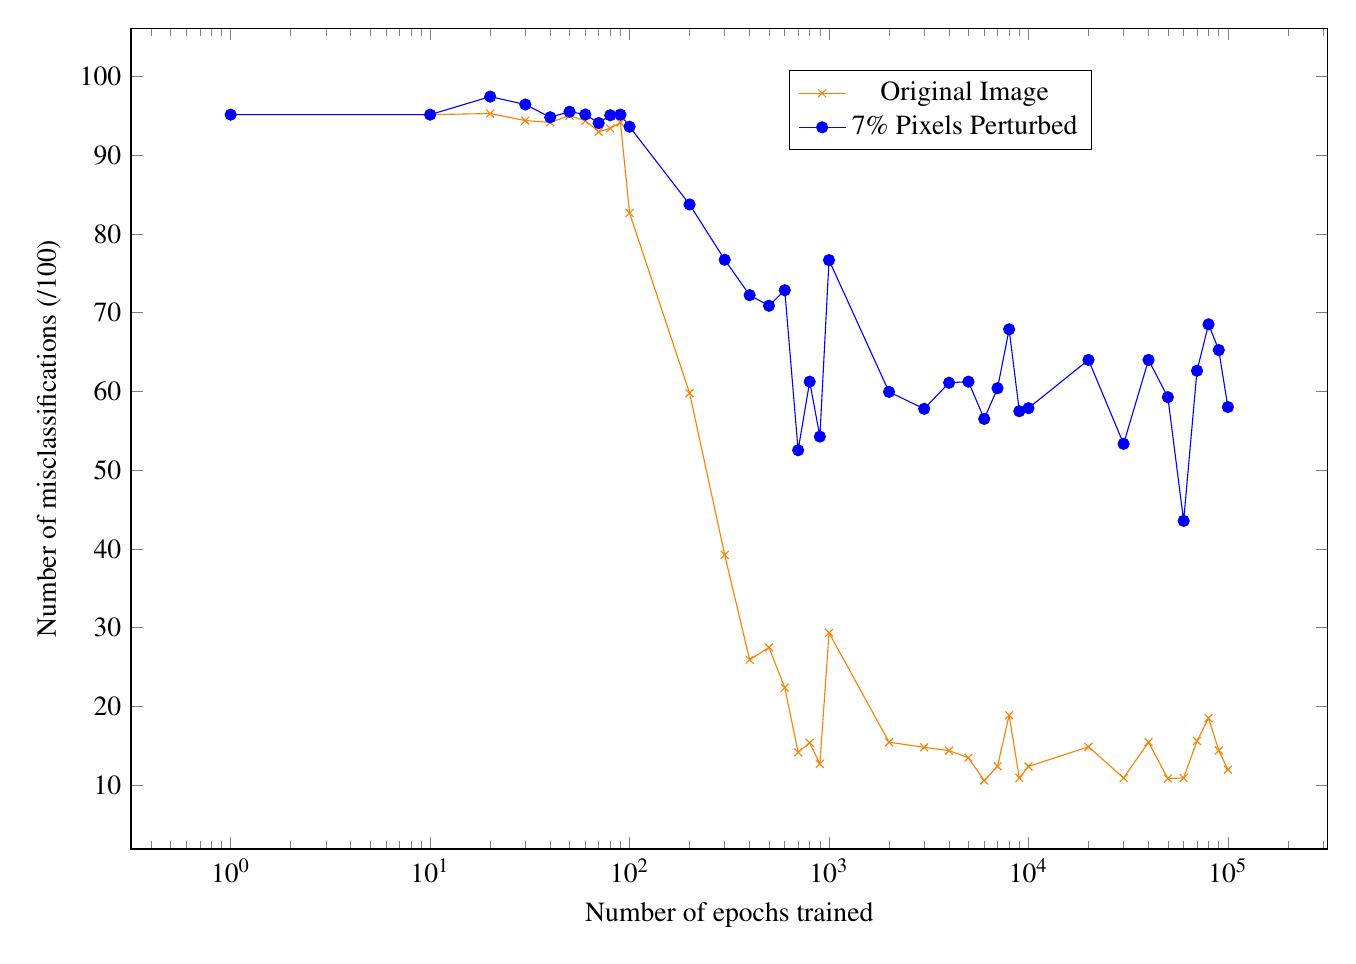
\begin{tikzpicture}
\begin{semilogxaxis}[
xlabel={Number of epochs trained},
ylabel={Number of misclassifications (/100)},
x=1.1cm,
y=1.0mm, 
legend style={at={(0.55,0.9)},anchor=west}]

\addplot[color=orange,mark=x] coordinates {
	(1, 95.159996)
	(10, 95.159996)
	(20, 95.300003)
	(30, 94.410004)
	(40, 94.180000)
	(50, 95.019997)
	(60, 94.389999)
	(70, 93.000000)
	(80, 93.419998)
	(90, 94.159996)
	(100, 82.669998)
	(200, 59.790001)
	(300, 39.240002)
	(400, 25.930000)
	(500, 27.490000)
	(600, 22.389999)
	(700, 14.180000)
	(800, 15.390000)
	(900, 12.700000)
	(1000, 29.359999)
	(2000, 15.460000)
	(3000, 14.810000)
	(4000, 14.390000)
	(5000, 13.490000)
	(6000, 10.590000)
	(7000, 12.400000)
	(8000, 18.889999)
	(9000, 10.920000)
	(10000, 12.380000)
	(20000, 14.880000)
	(30000, 10.920000)
	(40000, 15.460000)
	(50000, 10.850000)
	(60000, 10.920000)
	(70000, 15.620001)
	(80000, 18.520000)
	(90000, 14.410000)
	(100000, 11.980000)
};

\addplot[color=blue,mark=*] coordinates {
	(1, 95.159996)
	(10, 95.159996)
	(20, 97.450005)
	(30, 96.450005)
	(40, 94.830002)
	(50, 95.529999)
	(60, 95.180000)
	(70, 94.089996)
	(80, 95.089996)
	(90, 95.159996)
	(100, 93.629997)
	(200, 83.750000)
	(300, 76.729996)
	(400, 72.239998)
	(500, 70.889999)
	(600, 72.860001)
	(700, 52.540001)
	(800, 61.250000)
	(900, 54.280003)
	(1000, 76.689995)
	(2000, 59.950001)
	(3000, 57.799999)
	(4000, 61.109997)
	(5000, 61.250000)
	(6000, 56.520000)
	(7000, 60.420002)
	(8000, 67.900002)
	(9000, 57.500000)
	(10000, 57.889999)
	(20000, 64.010002)
	(30000, 53.349998)
	(40000, 64.010002)
	(50000, 59.280003)
	(60000, 43.570000)
	(70000, 62.639999)
	(80000, 68.529999)
	(90000, 65.259995)
	(100000, 58.029999)
};


\legend{Original Image, 7\% Pixels Perturbed}
\end{semilogxaxis}%
\end{tikzpicture}%}
	\caption{Line graph showing the effect of input perturbations on the prediction accuracy of a \ac{MNN} \label{fig:sign-graph-acc}}
\end{figure}

%\begin{figure}[t]
%	\centering
%	\scalebox{0.9}{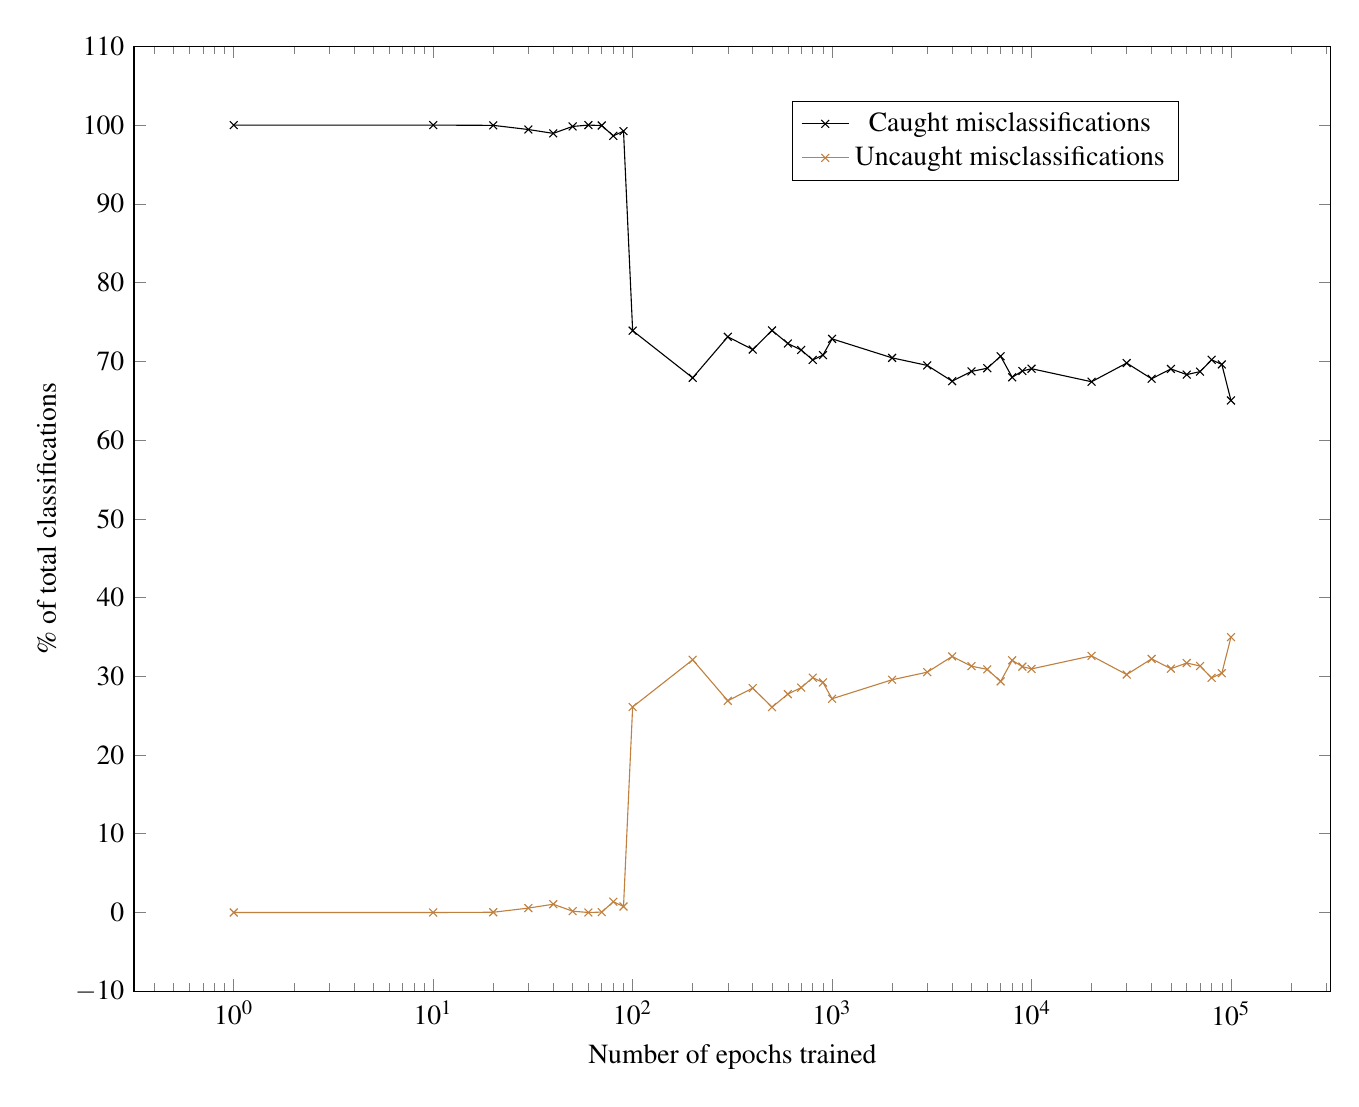
\begin{tikzpicture}
\begin{semilogxaxis}[
xlabel={Number of epochs trained},
ylabel={\% of total classifications},
x=1.1cm,
y=1.0mm, 
legend style={at={(0.55,0.9)},anchor=west}]

\addplot[color=black,mark=x] coordinates {
	(1, 100.000000)
	(10, 100.000000)
	(20, 99.968513)
	(30, 99.438622)
	(40, 98.948822)
	(50, 99.831619)
	(60, 100.000000)
	(70, 99.946243)
	(80, 98.629845)
	(90, 99.235352)
	(100, 73.896217)
	(200, 67.904327)
	(300, 73.114166)
	(400, 71.500191)
	(500, 73.917786)
	(600, 72.264412)
	(700, 71.438644)
	(800, 70.175438)
	(900, 70.787399)
	(1000, 72.854225)
	(2000, 70.439842)
	(3000, 69.480080)
	(4000, 67.477409)
	(5000, 68.717560)
	(6000, 69.121811)
	(7000, 70.645164)
	(8000, 67.972473)
	(9000, 68.772896)
	(10000, 69.063011)
	(20000, 67.405907)
	(30000, 69.780220)
	(40000, 67.787842)
	(50000, 69.032257)
	(60000, 68.315018)
	(70000, 68.693977)
	(80000, 70.194382)
	(90000, 69.604439)
	(100000, 65.025040)
};

\addplot[color=brown,mark=x] coordinates {	
	(1, 0.000000)
	(10, 0.000000)
	(20, 0.031486)
	(30, 0.561380)
	(40, 1.051184)
	(50, 0.168381)
	(60, 0.000000)
	(70, 0.053759)
	(80, 1.370155)
	(90, 0.764649)
	(100, 26.103786)
	(200, 32.095673)
	(300, 26.885832)
	(400, 28.499805)
	(500, 26.082212)
	(600, 27.735594)
	(700, 28.561354)
	(800, 29.824560)
	(900, 29.212601)
	(1000, 27.145777)
	(2000, 29.560154)
	(3000, 30.519920)
	(4000, 32.522587)
	(5000, 31.282434)
	(6000, 30.878185)
	(7000, 29.354836)
	(8000, 32.027523)
	(9000, 31.227106)
	(10000, 30.936995)
	(20000, 32.594090)
	(30000, 30.219782)
	(40000, 32.212166)
	(50000, 30.967743)
	(60000, 31.684982)
	(70000, 31.306025)
	(80000, 29.805618)
	(90000, 30.395559)
	(100000, 34.974957)
};


\legend{Caught misclassifications, Uncaught misclassifications}
\end{semilogxaxis}%
\end{tikzpicture}%}
%	\caption{Line graph showing the performance of the system trained over an increasing amount of epochs using unperturbed inputs \label{fig:sign-graph}}
%\end{figure}

%\begin{figure}[t]
%	\centering
%	\scalebox{0.9}{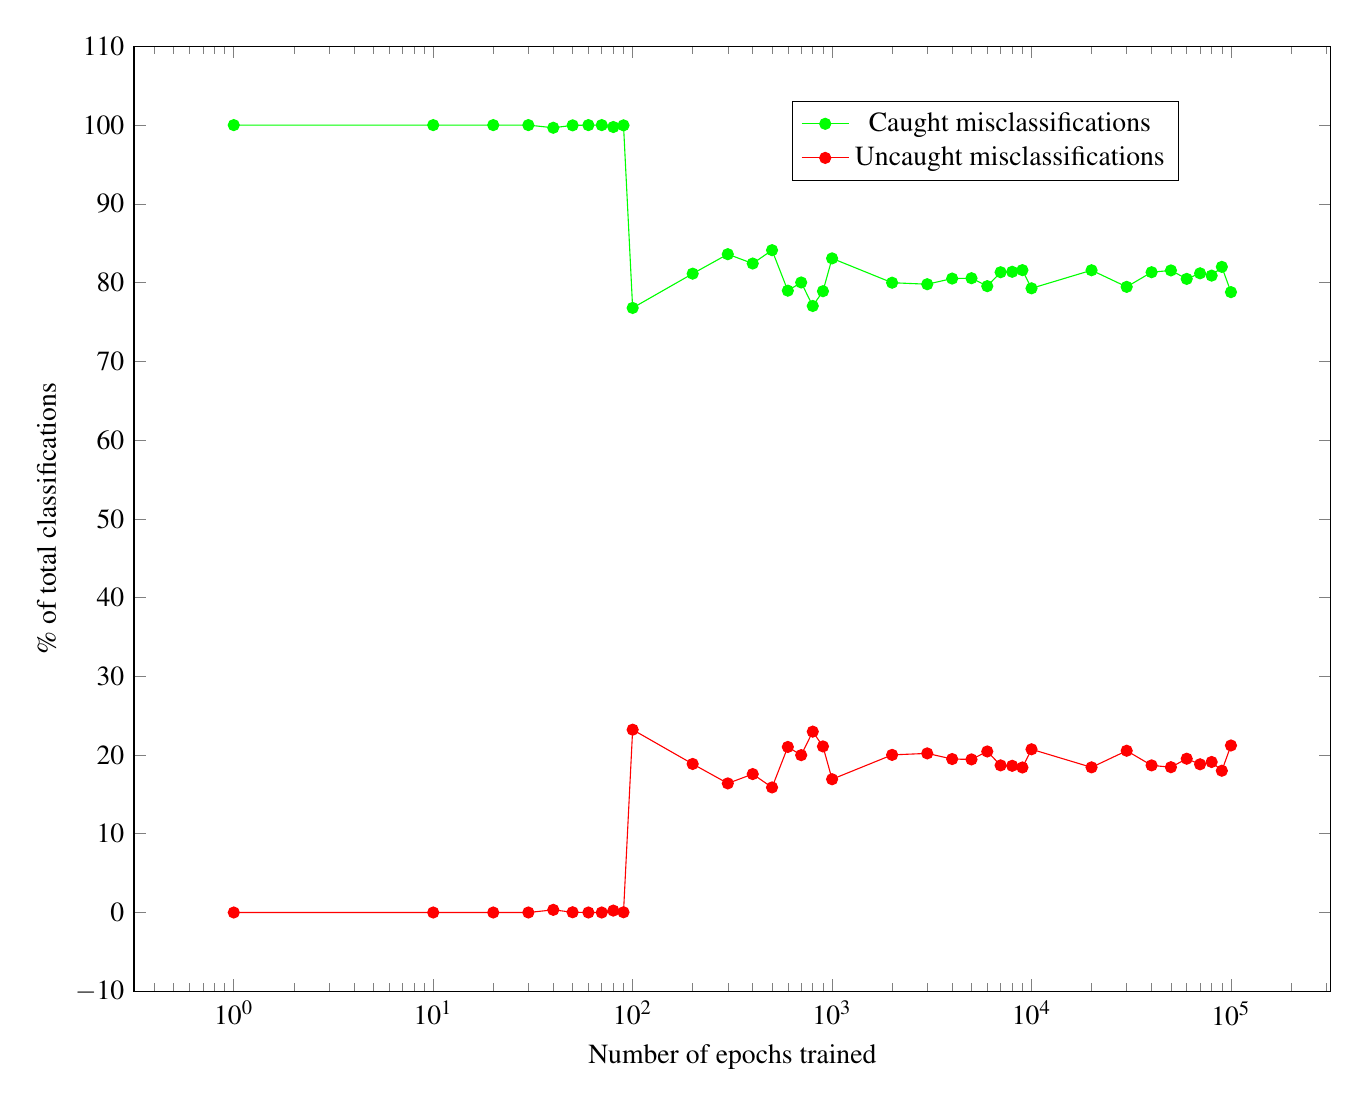
\begin{tikzpicture}
\begin{semilogxaxis}[
xlabel={Number of epochs trained},
ylabel={\% of total classifications},
x=1.1cm,
y=1.0mm, 
legend style={at={(0.55,0.9)},anchor=west}]

\addplot[color=green,mark=*] coordinates {	
	(1, 100.000000)
	(10, 100.000000)
	(20, 100.000000)
	(30, 100.000000)
	(40, 99.662552)
	(50, 99.968597)
	(60, 100.000000)
	(70, 100.000000)
	(80, 99.758133)
	(90, 99.968475)
	(100, 76.780945)
	(200, 81.134331)
	(300, 83.604851)
	(400, 82.419716)
	(500, 84.116234)
	(600, 78.973373)
	(700, 80.015221)
	(800, 77.028572)
	(900, 78.905663)
	(1000, 83.074722)
	(2000, 79.983315)
	(3000, 79.792389)
	(4000, 80.510559)
	(5000, 80.555107)
	(6000, 79.547066)
	(7000, 81.314125)
	(8000, 81.369659)
	(9000, 81.582603)
	(10000, 79.271027)
	(20000, 81.565376)
	(30000, 79.456421)
	(40000, 81.315414)
	(50000, 81.545204)
	(60000, 80.468216)
	(70000, 81.178162)
	(80000, 80.884285)
	(90000, 81.995102)
	(100000, 78.786835)
};

\addplot[color=red,mark=*] coordinates {
	(1, 0.000000)
	(10, 0.000000)
	(20, 0.000000)
	(30, 0.000000)
	(40, 0.337446)
	(50, 0.031402)
	(60, 0.000000)
	(70, 0.000000)
	(80, 0.241872)
	(90, 0.031525)
	(100, 23.219051)
	(200, 18.865665)
	(300, 16.395145)
	(400, 17.580284)
	(500, 15.883766)
	(600, 21.026627)
	(700, 19.984774)
	(800, 22.971428)
	(900, 21.094332)
	(1000, 16.925280)
	(2000, 20.016680)
	(3000, 20.207613)
	(4000, 19.489441)
	(5000, 19.444899)
	(6000, 20.452932)
	(7000, 18.685873)
	(8000, 18.630341)
	(9000, 18.417391)
	(10000, 20.728970)
	(20000, 18.434624)
	(30000, 20.543579)
	(40000, 18.684584)
	(50000, 18.454794)
	(60000, 19.531784)
	(70000, 18.821840)
	(80000, 19.115713)
	(90000, 18.004898)
	(100000, 21.213161)
};

\legend{Caught misclassifications, Uncaught misclassifications}
\end{semilogxaxis}%
\end{tikzpicture}%}
%	\caption{Line graph showing the number of misclassifications made by the system with perturbed inputs \label{fig:sign-graphpert}}
%\end{figure}

\begin{figure}[t]
	\centering
	\scalebox{0.9}{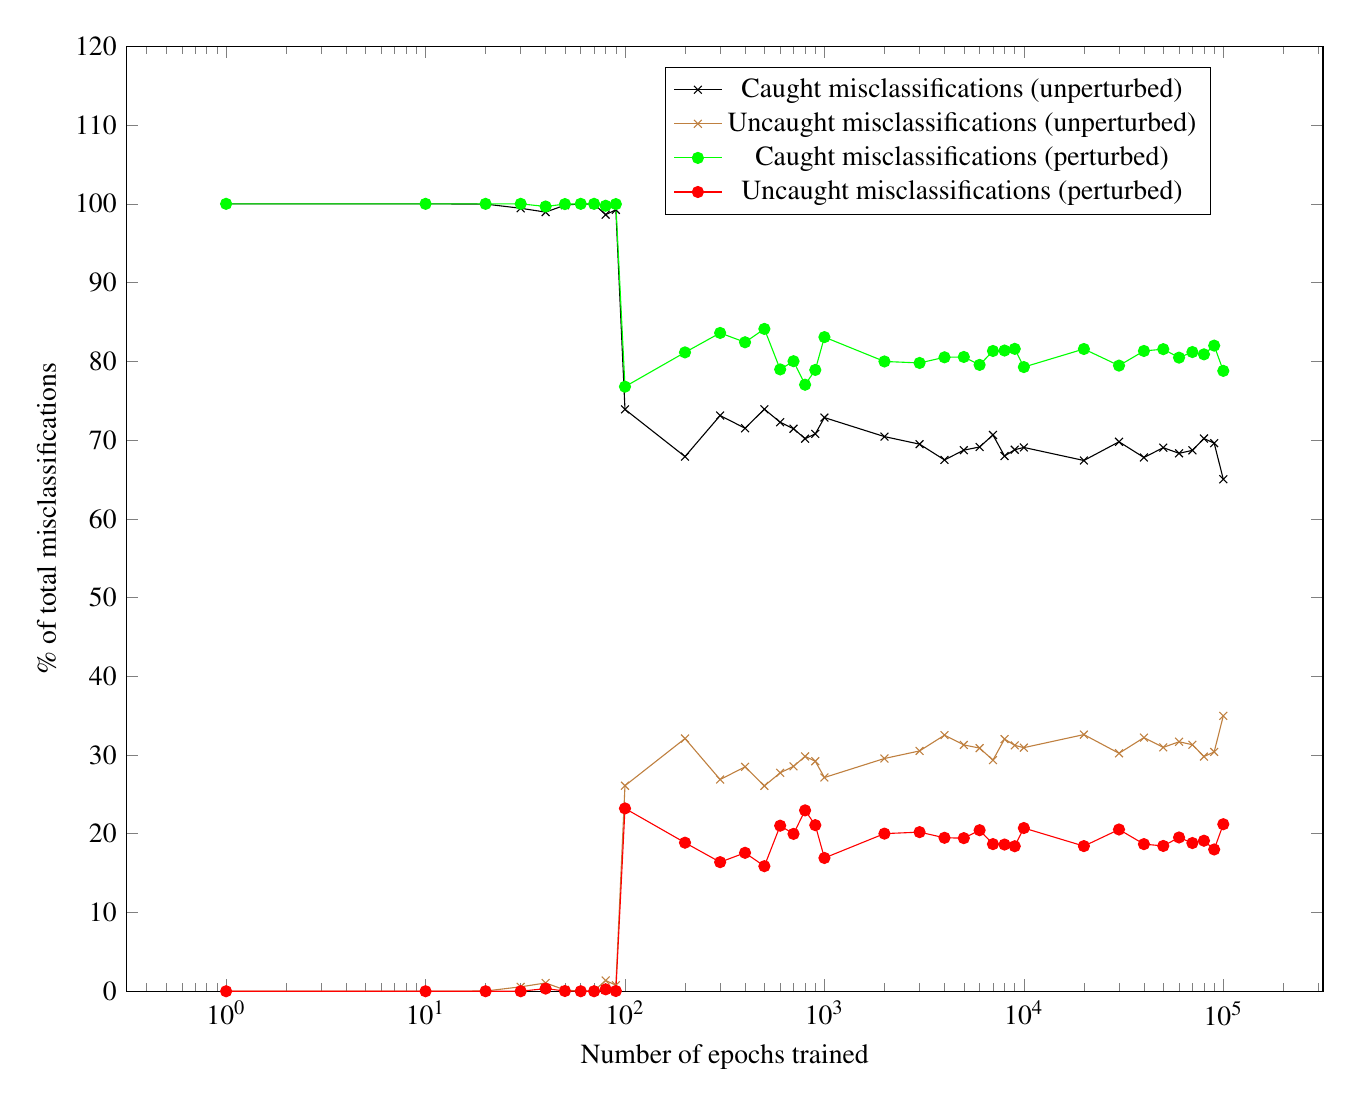
\begin{tikzpicture}
\begin{semilogxaxis}[
xlabel={Number of epochs trained},
ylabel={\% of total misclassifications},
x=1.1cm, y=1.0mm, 
ymin=0, ymax=120,
legend style={at={(0.45,0.9)},anchor=west}]

\addplot[color=black,mark=x] coordinates {
	(1, 100.000000)
	(10, 100.000000)
	(20, 99.968513)
	(30, 99.438622)
	(40, 98.948822)
	(50, 99.831619)
	(60, 100.000000)
	(70, 99.946243)
	(80, 98.629845)
	(90, 99.235352)
	(100, 73.896217)
	(200, 67.904327)
	(300, 73.114166)
	(400, 71.500191)
	(500, 73.917786)
	(600, 72.264412)
	(700, 71.438644)
	(800, 70.175438)
	(900, 70.787399)
	(1000, 72.854225)
	(2000, 70.439842)
	(3000, 69.480080)
	(4000, 67.477409)
	(5000, 68.717560)
	(6000, 69.121811)
	(7000, 70.645164)
	(8000, 67.972473)
	(9000, 68.772896)
	(10000, 69.063011)
	(20000, 67.405907)
	(30000, 69.780220)
	(40000, 67.787842)
	(50000, 69.032257)
	(60000, 68.315018)
	(70000, 68.693977)
	(80000, 70.194382)
	(90000, 69.604439)
	(100000, 65.025040)
};

\addplot[color=brown,mark=x] coordinates {	
	(1, 0.000000)
	(10, 0.000000)
	(20, 0.031486)
	(30, 0.561380)
	(40, 1.051184)
	(50, 0.168381)
	(60, 0.000000)
	(70, 0.053759)
	(80, 1.370155)
	(90, 0.764649)
	(100, 26.103786)
	(200, 32.095673)
	(300, 26.885832)
	(400, 28.499805)
	(500, 26.082212)
	(600, 27.735594)
	(700, 28.561354)
	(800, 29.824560)
	(900, 29.212601)
	(1000, 27.145777)
	(2000, 29.560154)
	(3000, 30.519920)
	(4000, 32.522587)
	(5000, 31.282434)
	(6000, 30.878185)
	(7000, 29.354836)
	(8000, 32.027523)
	(9000, 31.227106)
	(10000, 30.936995)
	(20000, 32.594090)
	(30000, 30.219782)
	(40000, 32.212166)
	(50000, 30.967743)
	(60000, 31.684982)
	(70000, 31.306025)
	(80000, 29.805618)
	(90000, 30.395559)
	(100000, 34.974957)
};

\addplot[color=green,mark=*] coordinates {	
	(1, 100.000000)
	(10, 100.000000)
	(20, 100.000000)
	(30, 100.000000)
	(40, 99.662552)
	(50, 99.968597)
	(60, 100.000000)
	(70, 100.000000)
	(80, 99.758133)
	(90, 99.968475)
	(100, 76.780945)
	(200, 81.134331)
	(300, 83.604851)
	(400, 82.419716)
	(500, 84.116234)
	(600, 78.973373)
	(700, 80.015221)
	(800, 77.028572)
	(900, 78.905663)
	(1000, 83.074722)
	(2000, 79.983315)
	(3000, 79.792389)
	(4000, 80.510559)
	(5000, 80.555107)
	(6000, 79.547066)
	(7000, 81.314125)
	(8000, 81.369659)
	(9000, 81.582603)
	(10000, 79.271027)
	(20000, 81.565376)
	(30000, 79.456421)
	(40000, 81.315414)
	(50000, 81.545204)
	(60000, 80.468216)
	(70000, 81.178162)
	(80000, 80.884285)
	(90000, 81.995102)
	(100000, 78.786835)
};

\addplot[color=red,mark=*] coordinates {
	(1, 0.000000)
	(10, 0.000000)
	(20, 0.000000)
	(30, 0.000000)
	(40, 0.337446)
	(50, 0.031402)
	(60, 0.000000)
	(70, 0.000000)
	(80, 0.241872)
	(90, 0.031525)
	(100, 23.219051)
	(200, 18.865665)
	(300, 16.395145)
	(400, 17.580284)
	(500, 15.883766)
	(600, 21.026627)
	(700, 19.984774)
	(800, 22.971428)
	(900, 21.094332)
	(1000, 16.925280)
	(2000, 20.016680)
	(3000, 20.207613)
	(4000, 19.489441)
	(5000, 19.444899)
	(6000, 20.452932)
	(7000, 18.685873)
	(8000, 18.630341)
	(9000, 18.417391)
	(10000, 20.728970)
	(20000, 18.434624)
	(30000, 20.543579)
	(40000, 18.684584)
	(50000, 18.454794)
	(60000, 19.531784)
	(70000, 18.821840)
	(80000, 19.115713)
	(90000, 18.004898)
	(100000, 21.213161)
};

\legend{Caught misclassifications (unperturbed), Uncaught misclassifications (unperturbed), Caught misclassifications (perturbed), Uncaught misclassifications (perturbed)}
\end{semilogxaxis}%
\end{tikzpicture}%}
	\caption{Line graph showing the number of misclassifications caught by the enforcer \label{fig:sign-graphboth}}
\end{figure}

\subsection{An \ac{AV} System Using \acf{MNN2C}}
\ac{MNN2C}, introduced in Section~\ref{sec:mnn2c}, creates time-predictable, modular \acfp{MNN} for C from existing Keras (with Tensorflow) trained \acp{ANN}. 
This compiler makes implementing \acfp{MNN} in C easy and safe.
For the purposes of testing and demonstration, the complex \ac{MNN} used in this chapter, shown in Figure~\ref{fig:mnn}, was trained in Python, using Keras and the exact same images used to train the original system.
This \ac{MNN} was then described in the \ac{MNN2C} format, and modular C code was generated to initialise, run and incorporate the \ac{MNN}.
To show the efficacy of \ac{MNN2C}, the generated \ac{MNN} was implemented in an identical system to the original, and run with the same tests. 
It has already been shown that \ac{MNN2C} generates outputs identical to the Keras trained \acp{ANN} with a one hundred-thousandth tolerance, so the output of each individual \ac{SNN} is not being tested, rather that the system as a whole runs as the original does.

\subsubsection{Results of an \ac{MNN2C} Generated \ac{AV} System}
Figure~\ref{fig:sign-graphboth-mnn2c} shows that the enforcer stills runs perfectly fine with Keras trained \acp{MNN} compiled to C code.
The enforcer picked up more than 70\% of all misclassifications, catching more misclassifications as the training of the \acp{MNN} was increased. 
As the training increased, the \acp{MNN} become more confident with their predictions, and thus the enforcer is able to more accurately determine misclassifications.

Since these \acp{MNN} were trained in Keras, they did not need to go through extensive training to get to a reasonable classification accuracy, only needing 100 epochs to get to level as the Darknet \acp{MNN}.
The enforcer works very similarly for perturbed and unperturbed images, unlike the Darknet \acp{MNN}.
This is due to the effective training methods used by Keras, allowing for better trained \acp{MNN} even with input perturbations.

%\begin{figure}[t]
%	\centering
%	\scalebox{0.9}{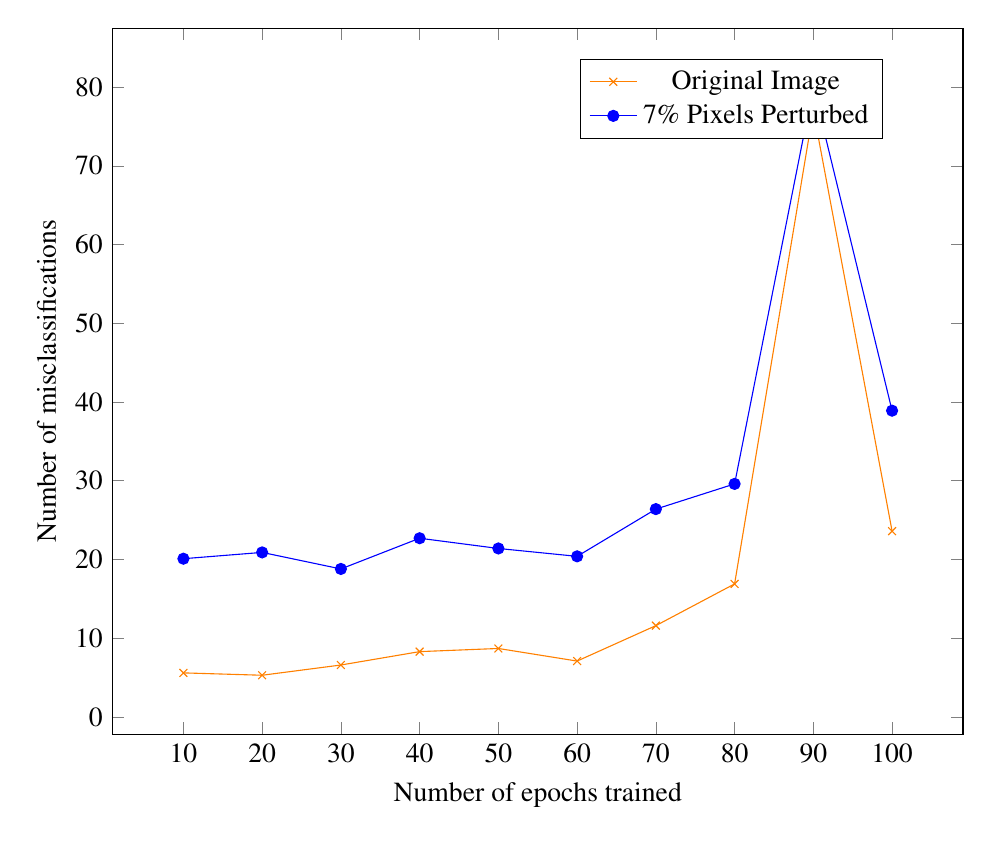
\begin{tikzpicture}
\begin{axis}[
xlabel={Number of epochs trained},
ylabel={Number of misclassifications},
x=1.0mm,
y=1.0mm, 
legend style={at={(0.55,0.9)},anchor=west}]

\addplot[color=orange,mark=x] coordinates {
	(10, 5.600000)
	(20, 5.300000)
	(30, 6.600000)
	(40, 8.300000)
	(50, 8.700000)
	(60, 7.100000)
	(70, 11.600000)
	(80, 16.900000)
	(90, 77.000000)
	(100, 23.600000)
	
};

\addplot[color=blue,mark=*] coordinates {
	(10, 20.100000)
	(20, 20.900000)
	(30, 18.799999)
	(40, 22.700001)
	(50, 21.400000)
	(60, 20.400000)
	(70, 26.400000)
	(80, 29.600000)
	(90, 80.000000)
	(100, 38.900002)
};


\legend{Original Image, 7\% Pixels Perturbed}
\end{axis}%
\end{tikzpicture}%}
%	\caption{Line graph showing the effect of input perturbations on the prediction accuracy of a \ac{SNN} \label{fig:sign-graph-acc-mnn2c}}
%\end{figure}

\begin{figure}[t]
	\centering
	\scalebox{0.9}{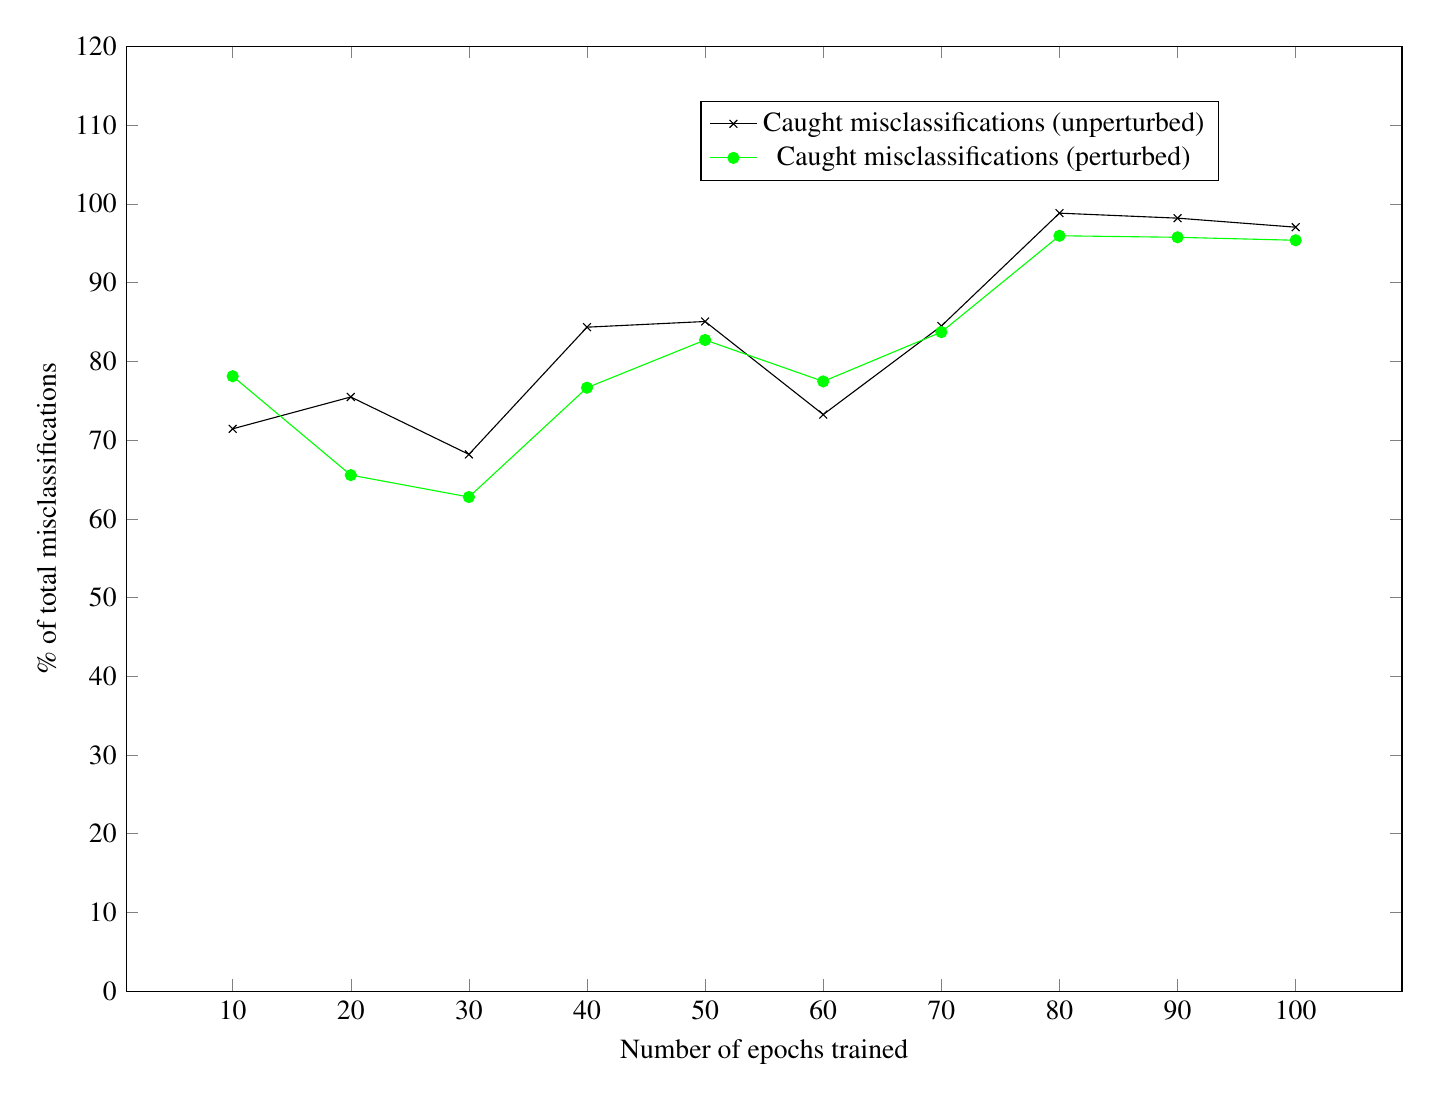
\begin{tikzpicture}
\begin{axis}[
xlabel={Number of epochs trained},
ylabel={\% of total misclassifications},
x=1.5mm, y=1.0mm, 
ymin=0, ymax=120,
legend style={at={(0.45,0.9)},anchor=west}]

\addplot[color=black,mark=x] coordinates {
	(10, 71.428574)
	(20, 75.471695)
	(30, 68.181816)
	(40, 84.337349)
	(50, 85.057472)
	(60, 73.239433)
	(70, 84.482758)
	(80, 98.816566)
	(90, 98.181816)
	(100, 97.033897)
};

\addplot[color=green,mark=*] coordinates {	
	(10, 78.109451)
	(20, 65.550240)
	(30, 62.765957)
	(40, 76.651985)
	(50, 82.710281)
	(60, 77.450981)
	(70, 83.712120)
	(80, 95.945946)
	(90, 95.750000)
	(100, 95.372749)
};

\legend{Caught misclassifications (unperturbed), Caught misclassifications (perturbed)}
\end{axis}%
\end{tikzpicture}%}
	\caption{Line graph showing the number of misclassifications caught by the enforcer with \ac{MNN2C} generated \acp{MNN} \label{fig:sign-graphboth-mnn2c}}
\end{figure}






















\section{Summary}
This chapter introduced the concept of \acfp{SNN} and their timing properties.

In Section~\ref{sec:motivating-example}, \acp{SNN} and their behaviour are introduced. 
Additionally, a motivating example is given with it's Esterel implementation.

Section~\ref{sec:wcrt} introduces the methods by which timing analysis is done on \acp{SNN} and the algebra involved with this.
This chapter also gives the first formal definition of a \ac{SNN} and discusses the periodicity of these \acp{SNN}.

The next section, Section~\ref{sec:concurrent-sann}, introduces the concept of \acfp{MNN} and provides formal definitions for them, as well as providing examples of the structure of the introduces \acp{MNN}.

A new Python compiler for creating \acp{MNN} from Keras is introduced in Section~\ref{sec:mnn2c} and its results are presented.

The final section of this chapter presents the results of the work done on \acp{SNN} and \acp{MNN} for this chapter.
These results are discussed and analysed, with conclusions drawn in the following chapter.

\section{Discussion}
\label{sec:conclusion}

In this work, we have presented an approach for synchronous composition of \acf{RE} with \acfp{ANN} for \acp{CPS} by defining \acfp{SNN}.
Our \acp{SNN} demonstrate that policies specifying safe I/O behaviours for \acp{ANN} can be enforced.
These enforced policies are shown to increase the safety and efficiency of the systems within which they are placed, without adding a large overhead to the system and without decreasing the functionality of the system.
In the three case studies presented, the \ac{RE} added an average overhead of just 6.035\%, but the efficiency and safety of each system was increased by an amount that rendered the overhead negligible.






\chapter{Conclusions}

In this thesis, we proposed the use of synchronous programming towards the safe use of \acfp{ANN} in \acfp{CPS}, which are safety-critical systems.
Using the synchronous programming language Esterel, \acfp{SNN}, were developed to create \acp{ANN} that maintained synchronous semantics.
We were able to create fully synchronous, predictable \acp{ANN} that were able to be used as the controllers in all our benchmarks.
The synchronous approach to \acp{ANN}, which includes formal definitions of the \acp{ANN}, simulations and implementations of \ac{CPS}, was demonstrated throughout this thesis.
The results and concerns of this approach are discussed.

Two different structure types were defined: \acp{SNN} and \acp{MNN}.
\acp{SNN} are \acp{ANN} that run in a synchronous manner and maintain synchronous semantics, while \acp{MNN} are compositions of multiple \acp{SNN}, also retaining synchronous semantics.
Using the time predictable T-CREST platform, a set of benchmarks were developed using Esterel and C to prove the efficacy of \acp{SNN} and \acp{MNN}. 
These benchmarks ranged from basic, \acfp{MLP} to larger, more complex \acfp{MNN}.
Static timing analysis was done on these benchmarks, proving that the implemented \acp{SNN} and \acp{MNN} were not only time predictable, but also that the system were able to meet real-time deadlines.
Additionally, a Python tool chain, termed \acf{MNN2C} was introduced.
This compiler was able to produce time-predictable, \acp{MNN} from existing Keras trained \acp{ANN}.
This tool chain produced more accurate, lower \acf{WCRT} measurements compared to the original \acp{MNN}.

The next body of work introduced the concept of combining \acf{RE} with \acp{MNN}.
To this end, the definition of a \ac{MNN} was expanded to include arbitrary synchronous components, such as run-time enforcer, and not \acp{SNN}.
These new \acp{MNN} were termed \acfp{SNN}.
An \ac{AV} case study was used to demonstrate the efficacy of run-time enforced \acp{SNN} by enforcing a set of safety policies to ensure the safe behaviour of an \ac{AV} when presented with dangerous situations.
This approach was shown to vastly increase the safety of an \ac{AV}, allowing the \ac{AV} to run autonomously for long periods of time.
However, a complication arose with the realisation that the I/O of an \ac{ANN} with complex inputs, such as a \acf{CNN}, cannot be enforced.

The issue of input perturbation, where the inputs to the system are altered beyond the control of the system, was addressed next.
We proposed the use of \acf{RV}, sensor fusion and \acp{SNN} to decrease the risk posed by input perturbation.
To show the effect of input perturbation, and test our approach to addressing it, a different \ac{AV} system was created. 
This system was a simulation of the object classifier in an \ac{AV}, i.e. the part of the controller responsible for identifying the \ac{AV}'s surrounding environment.
Perturbed inputs were shown to decrease the classification accuracy of the system by up to 50\%, however our solution showed that \ac{RV} was able to ``catch'' more than 70\% of all misclassification, and when the inputs perturbation occurred the \ac{RV} was able to ``catch'' more than 80\% of the misclassifications.
Using the \ac{MNN2C} tool, this approach was tested on Keras generated \acp{SNN}.
These \acp{SNN} produced the same results, showing that more than 70\% of all misclassifications were detected by the \ac{RV}.

\section{Future Work}

While synchronous, time predictable \acp{ANN} proved to be of great value, they were only implemented and tested using C on single core processors.
The multi-core implementation and timing was not covered in thesis, but was researched with the construction of \ac{MNN2C}.
More research is required to the efficient multi-core implementations of \acp{SNN} for embedded systems.
Additionally, the hardware implementation of \acp{SNN} was not researched for this thesis, but is also a key bit of research.
\acp{SNN} have the potential to be implemented on a whole range of hardware, from \acfp{FPGA} to graphics cards.
This needs to be carefully researched. 

This thesis suggested \ac{RE} as an approach to creating safe \acp{ANN}, however only a single run-time enforcer was used in each benchmark.
While this was shown to be largely effective, this is not the limit to which \ac{RE} can be used in these \acp{SNN}.
In this thesis, we did not fully examine the enforcement of multiple networks in a \ac{SNN}, nor did we fully investigate all the possible compositions and combinations of \ac{RE} and \acp{MNN}.
Examining more compositions of \acp{SNN} with their run-time enforcers could lead to more capable systems that are still safe, or safer. 
Approaches such as using \ac{RE} during the training of \acp{SNN} has yet to be explored, and \ac{RE} between layers of individual \acp{SNN} has also yet to be explored.

Only the basics of \ac{RV} was discussed in this thesis.
\ac{RV} has a lot more value than just being used for \acp{CNN} in \ac{AV} systems.
This approach can be taken on any system where the inputs to the system are complex, such a intrusion detection system on networks. 
More benchmarks should be developed that expand on a lot more \ac{CPS} that could benefit from \ac{RV}.

Lastly, the composition of \acp{SNN} was not fully researched in this thesis.
The training phase of \acp{SNN} was skipped, instead each \ac{ANN} was trained individually.
\acp{SNN} are a unique composition of \acp{SNN} and other synchronous components, and the training of such systems needs further investigation.
Additionally, the only structure of \ac{SNN} used in this thesis was a \ac{SNN} ensemble, where each \ac{SNN} in the ensemble works with the others in the ensemble to provide more accurate output.
There exist endless ways that \acp{SNN} can be combined, and more of these ways should be implemented and tested.













\appendix
\chapter{Appendix}


%\include{Publications}


%%%%%%%%%%%% Last part of thesis indices, bibliography  %%%%%%%%%%%%
\backmatter

%create the bibliography
% \bibliographystyle{siam}
\renewcommand{\bibname}{References}
% \clearpage
\phantomsection
\addcontentsline{toc}{chapter}{\bibname}
\bibliographystyle{IEEEtranS}
\bibliography{references}


\end{document}

